\documentclass[letterpaper,12pt, twoside]{book}
\usepackage[spanish]{babel}
\usepackage[T1]{fontenc}
\usepackage[utf8]{inputenc}
\usepackage{graphicx}
\usepackage{amsfonts,amsmath,color,amssymb,float, amsthm,mathrsfs}  
\usepackage[top=2cm,bottom=1.5cm, inner=2cm, outer=4.5cm,includeheadfoot, headheight=16pt]{geometry}
% \usepackage[showframe,headsep=1cm,headheight=2cm, top=2cm, right=3cm,left=2cm,includeheadfoot]{geometry}
\usepackage{wrapfig} 
\usepackage{framed}
\usepackage[most]{tcolorbox}
\usepackage[svgnames]{xcolor} 
\colorlet{shadecolor}{green!20}
\setlength\FrameSep{0.5ex}
\usepackage{thmtools}
\usepackage{esint}
\usepackage{cancel}
\usepackage{listings} 
\usepackage{pstricks}
\usepackage{csquotes}
\usepackage{enumitem}
\usepackage{etoolbox}
\usepackage{tikz}
\usepackage{multicol}
\usetikzlibrary{arrows,babel}
\usepackage[font=small]{caption}
\usepackage{mathtools}
\usepackage{float}
\usepackage{subcaption}

\usepackage{marginnote}
\renewcommand*{\marginfont}{\bfseries\footnotesize}

\frenchspacing

\decimalpoint
\newcommand{\grad}{^\circ}
\newlength{\drop}
\DeclareMathOperator{\sign}{sgn}
\DeclareMathOperator{\Log}{Log}
\providecommand{\norm}[1]{\lVert#1\rVert}
\DeclareMathOperator{\real}{Re}
\DeclareMathOperator{\im}{Im}





%%%%%%%%%%%%%%%%%%%%%%%%%%%%%%%%%%%%%%%%%%%%%%

%%%%%%%%%%%%Fancy Chapters%%%%%%%%%%%%%%%%%
%Options: Sonny, Lenny, Glenn, Conny, Rejne, Bjarne, Bjornstrup
\usepackage[Bjornstrup]{fncychap}

\usepackage[default]{sourcesanspro}
\usepackage{libertinust1math}
\usepackage{montserrat}

\ChTitleVar{\bfseries\LARGE\sffamily\fontfamily{Montserrat-LF}\selectfont}
%%%%%%%%%%%%%%%%%%%%%%%%%%%%%%%%%%%%%%%%%%%

\usepackage{fancyhdr}

\fancyhead[LO, RE]{\thepage}
\fancyhead[LE]{\leftmark}
\fancyhead[RO]{\rightmark}
\fancyfoot{}

\fancypagestyle{plain}{
  \fancyhead[LO, RE]{\thepage}
  \renewcommand{\headrulewidth}{0pt}
}

\usepackage{xpatch}
\newlength{\chaptertopskip}
\setlength{\chaptertopskip}{10pt}
\makeatletter
\xpatchcmd{\@makechapterhead}{\vspace*{50\p@}}{\vspace*{\chaptertopskip}}{\typeout{Success}}{\typeout{Failure!!!}}
\makeatother

\makeatletter
\renewcommand{\section}{%
  \@startsection{section}{1}{0mm}% Nombre, nivel, sangría
  {1.5\baselineskip}% Espacio antes
  {0.5\baselineskip}% Espacio después
  {\Large\bfseries\sffamily\fontfamily{Montserrat-LF}\selectfont}} % Formato
\makeatother

\makeatletter
\renewcommand{\subsection}{%
  \@startsection{subsection}{2}{0mm}% Nombre, nivel, sangría
  {1.2\baselineskip}% Espacio antes
  {0.3\baselineskip}% Espacio después
  {\large\bfseries\sffamily\fontfamily{Montserrat-LF}\selectfont}} % Formato
\makeatother

%%%%%%%%% Modificamos la forma de los títulos

%%% ******************************************************* added
\definecolor{titlechap}{HTML}{FEF8F8} % color of the chapter title <<<
\definecolor{numberchap}{HTML}{000945}% color of the chapter number <<<<
\definecolor{left}{HTML}{2B7EA0}
\definecolor{right}{HTML}{2a9d8f}
\definecolor{righter}{HTML}{6EBCB2}

\usepackage{tikz}
\usetikzlibrary{fadings,positioning}
\newcommand{\gradient}[1]{
  \begin{tikzpicture}
    \node (rect) at (0,0) [shade, left color=left,middle color=right, right color=white,minimum width=17cm,minimum height=2.5cm] {};
    \node(title)[above left = 10pt and -10pt of rect.south west, anchor=south west, font=\CTV, text width=14cm] {\textcolor{titlechap}{#1}};
    \ifnum\value{chapter}>0 \node[left = 5pt of rect.north east,  anchor=center, font=\CNoV] {\textcolor{numberchap!80}{\thechapter}};\fi%
\end{tikzpicture}%
\vskip 40pt%
}

\renewcommand{\DOCH}{}
\renewcommand{\DOTI}[1]{\gradient{#1}}
\renewcommand{\DOTIS}[1]{\gradient{#1}}

%%%%%%%%%%%%%%%%%%%%%%%

%%%%%%%%%Entornos: Teoremas, Defs,etc%%%%%%%
\theoremstyle{definition}

\definecolor{MyPurple}{HTML}{44006C}

\newtheorem{defis}{Definiciones}[section]
\newtheorem{corolario}{Corolario}[section] 

\newtheorem{protoexample}{Ejemplo}[chapter]
\newenvironment{ejemplo}
   {\colorlet{shadecolor}{righter!15}\begin{shaded}\begin{protoexample}}
   {\end{protoexample}\end{shaded}}

\newtheorem*{protoproof}{Demostración}
\newenvironment{demo}
   {\colorlet{shadecolor}{blue!10}\begin{shaded}\begin{protoproof}}
   {\end{protoproof} \end{shaded}}

\newenvironment{Rdbleftbar}{%
  \def\FrameCommand{\textcolor{MyPurple!80}{\vrule width0.6pt}\hspace{0.15em}\textcolor{MyPurple!80}{\vrule width0.6pt} \hspace{0.5em}}%
  \MakeFramed {\advance\hsize-\width \FrameRestore}}%
 {\endMakeFramed}

 \newenvironment{Bdbleftbar}{%
  \def\FrameCommand{\textcolor{left}{\vrule width0.6pt}\hspace{0.15em}\textcolor{left}{\vrule width0.6pt}\hspace{0.5em}}%
  \MakeFramed {\advance\hsize-\width \FrameRestore}}%
 {\endMakeFramed}

\newenvironment{Gdbleftbar}{%
  \def\FrameCommand{\textcolor{right!80}{\vrule width0.6pt}\hspace{0.15em}\textcolor{right!80}{\vrule width0.6pt} \hspace{0.5em}}%
  \MakeFramed {\advance\hsize-\width \FrameRestore}}%
 {\endMakeFramed}
 
% With parskip

\usepackage[indent=0.6cm]{parskip}

\declaretheorem[%
name            =Teorema,%
numberwithin=chapter,
postheadhook    =\vspace*{\parskip} \begin{Rdbleftbar}\vspace*{-5pt},%
prefoothook     =\vspace*{-1pt}\end{Rdbleftbar}%
]{teorema}

\declaretheorem[%
name            =Definición,%
numberwithin=chapter,
postheadhook    =\vspace*{\parskip}\begin{Bdbleftbar}\vspace*{-5pt},%
prefoothook     =\vspace*{-1pt}\end{Bdbleftbar}%
]{defi}

\declaretheorem[%
name            = Proposición,%
numberwithin=chapter,
postheadhook    =\vspace*{\parskip}\begin{Gdbleftbar}\vspace*{-5pt},%
prefoothook     =\vspace*{-1pt}\end{Gdbleftbar}%
]{propo}  

\declaretheorem[%
name            = Propiedad,%
numberwithin=chapter,
postheadhook    =\vspace*{\parskip}\begin{Gdbleftbar}\vspace*{-5pt},%
prefoothook     =\vspace*{-1pt}\end{Gdbleftbar}%
]{propiedad}   

\newtcolorbox{obs}[2][]{enhanced,
  attach boxed title to top center={yshift=-3mm,yshifttext=-1mm},
  colback=right!5!white,
  colframe=left!75!black,
  colbacktitle=numberchap!80!white,
  title=#2,
  boxed title style={size=small,colframe=numberchap!50!black},
  #1
}

%Referencias
\usepackage[backend=biber]{biblatex}
\addbibresource{Referencias.bib}

\newcommand{\x}{\vec{x}}

% \usepackage[a-1b]{pdfx} % Permite compatibilidad con Chrome

\usepackage[colorlinks]{hyperref}

\usetikzlibrary{calc,shadows,shapes.geometric}

\newcommand{\breaktitle}{\texorpdfstring{\\}{ }}

\begin{document}

\frontmatter

\newgeometry{top=2cm,bottom=1.5cm, left=1.5cm, right=1.5cm}

\thispagestyle{empty}

\begin{tikzpicture}[remember picture,overlay]
  \fill[MyPurple!70!right] (current page.south west) rectangle (current page.north east);
  
  
  \node[rounded corners,fill=right!70,text =right!5,regular polygon,regular polygon sides=6, minimum size=2.5 cm,inner sep=0,ultra thick] at ($(current page.west)+(2.5,-5)$) {\LARGE \bfseries };
  
  \foreach \i in {2.5,...,20}
  {
      \node[rounded corners,right!60,draw,regular polygon,regular polygon sides=6, minimum size=\i cm,ultra thick] at ($(current page.west)+(2.5,-5)$) {} ;
  }
  
  \foreach \i in {0.5,...,18}
  {d
  \node[rounded corners,right!60,draw,regular polygon,regular polygon sides=5, minimum size=\i cm,ultra thick] at ($(current page.north west)+(2.5,0)$) {} ;
  }
  
  % \foreach \i in {0.5,...,22}
  % {
  % \node[rounded corners,right!75,draw,regular polygon,regular polygon sides=6, minimum size=\i cm,ultra thick] at ($(current page.north east)+(0,-9.5)$) {} ;
  % }
  
  \foreach \i in {21,...,6}
  {
  \node[left!65,rounded corners,draw,regular polygon,regular polygon sides=5, minimum size=\i cm,ultra thick] at ($(current page.south east)+(-0.2,-0.45)$) {} ;
  }
  
  
  \node[left, right!5, text width=0.725*\paperwidth, align=right, minimum height=3cm, rounded corners] at ($(current page.north east)+(-1,-8)$)
  {
  {\fontsize{25}{30} \selectfont \bfseries Notas de Clase}
  };

  \node[left, right!5, text width=0.725*\paperwidth, align=right, minimum height=3cm, rounded corners] at ($(current page.north east)+(-1,-9)$)
  {
  {\fontsize{25}{30} \selectfont \bfseries Métodos Matemáticos para Geofísicos}
  };
  
  \node[left, right!10, text width=0.625*\paperwidth, align=right, minimum height=2cm, rounded corners] at ($(current page.north east)+(-1,-12)$)
  {
  {\LARGE \textit{Pedro A. Contreras-Corral}}
  };
  
  \node[left, right!5, text width=0.625*\paperwidth, align=right, minimum height=2cm, rounded corners] at ($(current page.north east)+(-1,-13)$)
  {
  {\fontsize{15}{18}\selectfont Universidad de Concepción}
  };

      %   \node[mynode] at ($(current page.north east)+(-1,-6)$) {\fontsize{25}{30}\selectfont \textsc{\textbf{Apuntes de Física Matemática II}}};
      % \node[mynode] at ($(current page.north east)+(-1.5,-8)$) {\fontsize{20}{24}\selectfont \textit{Pedro A. Contreras-Corral}};
      % \node[mynode] at ($(current page.north east)+(-1.8,-10)$) {\fontsize{15}{18}\selectfont Concepción, Enero 2025};
      % \node[above right] at ($(current page.south west)+(5,5)$) {\includegraphics[scale=0.5]{}};

\end{tikzpicture}
  
\newpage

\thispagestyle{empty}


\newpage

\begin{titlepage}
 \drop=0.1\textheight
    \centering
    \vspace*{\baselineskip}
    \rule{\textwidth}{1.6pt}\vspace*{-\baselineskip}\vspace*{2pt}
    \rule{\textwidth}{0.4pt}\\[\baselineskip]
    {\scshape\bfseries\Huge\fontfamily{Montserrat-LF}\selectfont Notas de Clase} \\[0.2\baselineskip]
    {\scshape\bfseries\Huge\fontfamily{Montserrat-LF}\selectfont Métodos Matemáticos para Geofísicos} \\[0.2\baselineskip]
    \rule{\textwidth}{0.4pt}\vspace*{-\baselineskip}\vspace{3.2pt}
    \rule{\textwidth}{1.6pt}\\[\baselineskip]
    {\Large Por: \par}
{\large Pedro A. Contreras-Corral \par}
{\large Agosto 2025 \par}
\vfill
{\large Versión 1.4 \par}
\end{titlepage}

\mbox{} 
\vfill
Apuntes de Métodos Matemáticos para Geofísicos 

\textcopyright\ 2025, Pedro Contreras Corral % Derechos de autor


% Versión 1.0.0

Documento publicado bajo la licencia GPL v3.0.

Puedes ver los cambios realizados en diferentes versiones del documento \href{https://github.com/Pedroga-cc/MMG/blob/main/changelog.txt}{aquí}.

% Este documento es 

% This program is free software: you can redistribute it and/or modify
% it under the terms of the GNU General Public License as published by
% the Free Software Foundation, either version 3 of the License, or
% (at your option) any later version.
\vspace{1cm} 

\restoregeometry

\chapter*{Prefacio}

Este documento ha sido preparado por Pedro Contreras Corral como material de apoyo para el curso Métodos Matemáticos para Geofísicos. En cuanto a su contenido, se han utilizado como base las notas de clase del curso Física Matemática II del profesor Guillermo Rubilar, y las profesoras Ariana Muñoz e Ivana Sebestova, además de los apuntes preparado por Alejandro Saavedra como ayudante de esta última, y por Pedro Contreras como docente encargado el semestre 2025-1. También han sido utilizadas como referencia las diapositivas del profesor Roberto Navarro, quien dictó el curso de Métodos Matemáticos el año 2024, y las notas de clase de Física Matemática I del profesor José Barea.

También se han usado como base (en mayor o menor medida) los textos establecidos en la bibliografía, \emph{Mathematical Methods for Physicists} de Arfken, \emph{Mathematical Methods for Physics and Engineering} de Riley y \emph{Mathematical Physics} de Butkov. Junto a ellos, se han usado algunas ideas del libro \emph{Mathematical Physics, a Modern Introduction to its Foundations} de Hassani.

Es posible que este documento contenga algunos typos y errores menores. En caso de que estos se presenten, serán mencionados en clases para que puedan tomar notas al respecto, y serán corregidos en versiones posteriores del documento. De igual manera, algunas demostraciones no se encuentran escritas, de modo que derivo el detalle de ellas a las fuentes respectivas cuando lo considere necesario.
%  En versiones futuras de este documento se actualizarán estas ausencias.

Agradezco las contribuciones de Lixin Lai, Fernanda Mella y Amaro Díaz al facilitarme sus notas y el material del curso de la profesora Ivana Sebestova, así como los de José Huenchual por sus notas del curso de la profesora Ariana Muñoz. Además, agradezco a las y los estudiantes de la edición 2025 de Física Matemática II, por haberme permitido realizar correcciones mayores a los contenidos en algunos capítulos del apunte de dicho curso.

\newpage

\vspace*{10cm}

\vfill

\emph{\textquotedblleft ...El trabajo en equipo se convertirá en el método de investigación científica."}

\begin{flushright}
Atribuída a John Desmond Bernal.
\end{flushright}



\tableofcontents

\mainmatter

\pagestyle{fancy}

\chapter{Análisis Vectorial}

Hasta ahora, probablemente poseen una familiaridad trabajando con coordenadas cartesianas en el espacio $\mathbb{R}^3$. Para definir un punto en este sistema, utilizamos las coordenadas $(x,y,z)$, que corresponden a la proyección del vector posición $\x$ sobre cada uno de los ejes cartesianos, rectas perpendiculares entre sí. Si mantenemos constante una de estas coordenadas, definimos un \emph{plano} perpendicular al eje que se ha mantenido constante. 

De esta forma, un punto $P$ con coordenadas $(a,b,c)$ corresponde también a la intersección de los planos $x=a$, $y=b$, $z=c$, perpendiculares a los ejes $x$, $y$ y $z$, respectivamente.

En este sistema, superficies más generales pueden describirse implícitamente mediante expresiones del tipo $F(x,y,z) = c$, donde $c$ es un valor constante. Por ejemplo, una esfera de radio $R$ puede ser descrita por la expresión $x^2+y^2+z^2 = R^2$. Distintos valores de $c$ permiten describir una \emph{familia} de superficies, con la misma naturaleza, pero diferentes posiciones.

Antes de entrar más de lleno en la discusión, recordemos e introduzcamos algunas definiciones.

\begin{defi} \marginnote{Delta de Kronecker}
    Se denomina \textbf{delta de Kronecker} al elemento $\delta_{ij}$, definido en un espacio vectorial de $n$ dimensiones como
    \begin{equation}
        \delta_{ij} = \begin{dcases}
            1, \qquad i = j \\
            0, \qquad i \neq j
        \end{dcases} \ .
    \end{equation} 

    Este elemento puede representarse de forma matricial como la matriz identidad del espacio de dimensión $n$.
\end{defi}

\newpage

\begin{defi} \marginnote{Base ortonormal}
    Sea un conjunto de vectores unitarios $\left\{ \hat{e}_i\right\}_{i=1}^n$ de un espacio $n$-dimensional. Diremos que este forma una \textbf{base ortonormal} si al realizar el producto escalar entre elementos del conjunto, se cumple la relación
    \begin{equation}
        \hat{e}_i\cdot \hat{e}_j = \delta_{ij} \ ,
    \end{equation}
    donde $\delta_{ij}$ es la delta de Kronecker.
\end{defi}

\begin{defi} \marginnote{Vector posición}
    Dado un sistema coordenado en un espacio de $n$ dimensiones, podemos definir el \textbf{vector posición} $\vec{x}$, que une el origen del sistema con punto con coordenadas $x_i$, con $i = 1, 2, \dots, n$ como
\begin{equation} \label{eq:vector-posicion}
    \vec{x} = x_1 \hat{e}_1 + x_2 \hat{e}_2 + \dots + x_n \hat{e}_n = \sum_{i=1}^n x_i \hat{e}_i \ ,
\end{equation}
donde las \textbf{componentes del vector} en la base $\{ \hat{e}_i\}_{i=1}^n$ pueden expresarse como
\begin{equation}
    x_i = \vec{x} \cdot \hat{e}_i \ .
\end{equation}
\end{defi}

Durante este capítulo, nos limitaremos a trabajar en tres dimensiones, pues son las necesarias para describir la gran mayoría de los fenómenos físicos que pueden interesarnos.

\section{Coordenadas curvilíneas ortogonales}


Supongamos que existen tres superficies descritas por las ecuaciones
\begin{equation}
    q_1(x,y,z) = c_1 \, , \quad q_2(x,y,z) = c_2 \, , \quad q_3(x,y,z) = c_3 \ ,
\end{equation}
que se intersectan en el punto $P=(a,b,c)$. Es decir, la única solución que satisface simultáneamente las ecuaciones anteriores es $(x,y,z) = (a,b,c)$.

Si las funciones $q_i$ son monovaluadas y con derivadas continuas, entonces estas serán invertibles, y podremos definir una correspondencia entre las coordenadas cartesianas $(a,b,c)$ y los valores $(c_1,c_2,c_3)$.

\begin{defi}
    Se denominan \textbf{superficies coordenadas} a las funciones de la forma
    \begin{equation}
        q_i(x,y,z) = c_i \ ,
    \end{equation}
    donde $i = 1, 2, 3$, cuya intersección define un \textbf{sistema de coordenadas curvilíneas} $(q_1, q_2, q_3)$.
    
    % un punto $P$, con \textbf{coordenadas curvilíneas} $(q_1, q_2, q_3)$.

    Si la intersección es en ángulo recto \emph{para todos los puntos}, se dice que el sistema es \textbf{ortogonal}.
\end{defi}

De esta forma, dado un punto $P$ con coordenadas cartesianas $(a,b,c)$, y con coordenadas curvilíneas $(c_1, c_2, c_3)$, podemos establecer la relación 
\begin{equation}
    x(c_1, c_2, c_3) = a \, , \quad y(c_1, c_2, c_3) = b \, , \quad z(c_1, c_2, c_3) = c \ ,
\end{equation} 
y el vector posición $\x(x,y,z) = x \hat{\imath} + y \hat{\jmath} + z \hat{k}$ podrá expresarse como 
\begin{equation*}
    \x(q_1, q_2, q_3) = x(q_1, q_2, q_3) \hat{\imath} + y(q_1, q_2, q_3) \hat{\jmath} + z(q_1, q_2, q_3) \hat{k} \ .
\end{equation*}

¿Podremos expresar el vector posición en términos de vectores unitarios, tangentes a cada una de las superficies coordenadas?

\begin{defi}
    Se denominan \textbf{vectores direccionales}, denotados por $\vec{e}_i$, a aquellos que son \emph{tangentes} a las superficies coordenadas $q_i(x,y,z)$. Matemáticamente, escribimos 
    \begin{equation}
        \vec{e}_i = \frac{\partial \x}{\partial q_i} \ ,
    \end{equation} 
    donde $\x$ es el vector posición.
\end{defi}

\begin{defi}
    Se denominan \textbf{factores de escala} $h_i$ a los módulos de los vectores direccionales,
    \begin{equation}
        h_i = \left\| \frac{\partial \x}{\partial q_i} \right\| \ .
    \end{equation}
\end{defi}

De esta forma, el vector posición puede escribirse en términos del sistema de coordenadas curvilíneas como 
\begin{equation}
    \x(q_1, q_2, q_3) = R_1 \hat{e}_1 + R_2 \hat{e}_2 + R_3 \hat{e}_3 \ ,
\end{equation}
donde, en general, $(R_1, R_2, R_3) \neq (q_1, q_2, q_3)$, pues las componentes del vector en este nuevo sistema coordenado se obtienen como,
\begin{equation*}
    R_i = \x \cdot \hat{e}_i = \x \cdot \frac{\vec{e}_i}{h_i} \ .
\end{equation*}

\begin{obs}{Observación}
    Las coordenadas $q_i$ no necesariamente tendrán dimensiones de longitud. Para compensar esto, los factores de escala pueden tener alguna dimensión dada, de modo que el producto $h_i q_i$ sí tenga unidades de longitud.
\end{obs}

\newpage

\subsection{Elementos infinitesimales}

\begin{defi}
    Dado el vector posición $\x$ de un punto con coordenadas curvilíneas $(q_1, q_2, q_3)$, se define un \textbf{desplazamiento infinitesimal} o \textbf{elemento de longitud} como 
    \begin{equation}
        d\vec{x} = \frac{\partial \x}{\partial q_1} dq_1 + \frac{\partial \x}{\partial q_2} dq_2 + \frac{\partial \x}{\partial q_3} dq_3 = h_1 dq_1 \hat{e}_1 + h_2 dq_2 \hat{e}_2 + h_3 dq_3 \hat{e}_3 \ ,
    \end{equation}
    donde $\hat{e}_i = \vec{e}_i / h_i$.
\end{defi}

\begin{defi}
    Para un sistema de coordenadas curvilíneas \emph{ortogonales}, se define un \textbf{elemento de arco} en el sistema de coordenadas como 
    \begin{equation}
        ds^2 = d\x \cdot d\x = h_1^2 dq_1^2 + h_2^2 dq_2^2 + h_3^2 dq_3^2 \ .
    \end{equation}
\end{defi}

\begin{defi}
    Para un sistema de coordenadas curvilíneas ortogonales $(q_1, q_2, q_3)$, se definen los \textbf{elementos de superficie} ortogonales a la superficie $q_i$ como 
    \begin{equation}
        d\vec{S}_i = d\x_j \times d\x_k = h_j h_k (\hat{e}_j \times \hat{e}_k) dq_j dq_k \ ,
    \end{equation}
    o de forma más explícita, 
    \begin{align*}
        d\vec{S}_1 & = h_2 h_3 dq_2 dq_3 \hat{e}_1 \ , \\
        d\vec{S}_2 & = h_3 h_1 dq_3 dq_1 \hat{e}_2 \ , \\
        d\vec{S}_3 & = h_1 h_2 dq_1 dq_2 \hat{e}_3 \ .
    \end{align*}
\end{defi}

\begin{defi}
    Dado un sistema de coordenadas curvilíneas ortogonales, se define el \textbf{elemento de volumen} como 
    \begin{equation}
        dV = \left| d\x_1 \cdot (d\x_2 \times d\x_3) \right| = h_1 h_2 h_3 dq_1 dq_2 dq_3 \ .
    \end{equation}
\end{defi}

\subsection{Coordenadas cilíndricas}

En coordenadas cilíndricas $(\rho, \phi, z)$, el vector posición de un punto con coordenadas cartesianas $(x,y,z)$ puede representarse como 
\begin{equation}
    \x = \rho \cos \phi \hat{\imath} + \rho \sin \phi \hat{\jmath} + z \hat{k} \ ,
\end{equation}
de donde se deduce que la relación entre ambos sistemas es 
\begin{equation}
    \begin{array}{rcl}
        x & = & \rho \cos \phi \ , \\
        y & = & \rho \sin \phi \ , \\
        z & = & z \ ,
    \end{array}
\end{equation} 
donde $\rho \in [0, +\infty)$, $\phi \in [0, 2\pi]$, y $z \in (-\infty, +\infty)$.
% , o inversamente,
% \begin{equation}
%     \begin{array}{rcl}
%         \rho & = & \sqrt{x^2 + y^2} \ , \\
%         \phi & = & \tan^{-1}\left(\frac{y}{x}\right) \ , \\
%         z & = & z \ .
%     \end{array}
% \end{equation} 

A partir del vector posición, podemos obtener los vectores direccionales 
\begin{align}
    \vec{e}_\rho & = \frac{\partial \x}{\partial \rho} = \cos \phi \hat{\imath} + \sin \phi \hat{\jmath} \ , \\
    \vec{e}_\phi & = \frac{\partial \x}{\partial \phi} = -\rho \sin \phi  \hat{\imath} + \rho \cos \phi \hat{\jmath} \ , \\
    \vec{e}_z & = \frac{\partial \x}{\partial z} = \hat{k} \ ,
\end{align}
con respectivos factores de escala 
\begin{equation}
    h_\rho = 1 \, , \quad h_\phi = \rho \, , \quad h_z = 1 \ .
\end{equation}

Un elemento de longitud será dado por 
\begin{equation}
    d\x(\rho, \phi, z) = d\rho \hat{e}_\rho + \rho d\phi \hat{e}_\phi + dz \hat{e}_z \ ,
\end{equation}
y un elemento de volumen será
\begin{equation}
    dV(\rho, \phi, z) = \rho d\rho d\phi dz \ .
\end{equation}

\begin{figure}[htbp]
    \centering
    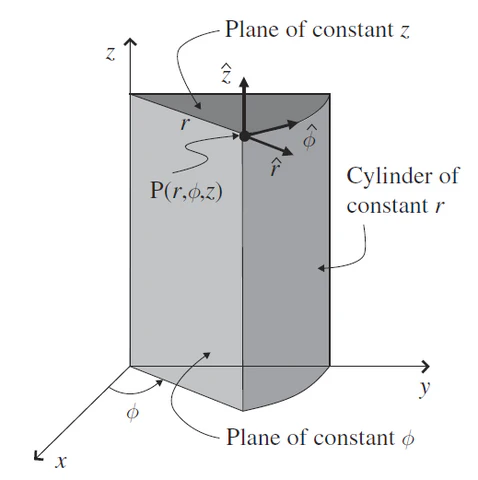
\includegraphics[width=8cm]{Figuras/Lineas-coordenadas-cilindricas.png}
    \caption{Sistema coordenado cilíndrico. Se puede apreciar que un punto en este es completamente determinado por la intersección de dos planos ($z =$ constante y $\phi = $ constante) y una superficie cilíndrica ($\rho = $ constante). Además, es posible apreciar la dirección de los tres vectores unitarios, $\hat{e}_\rho = \hat{\rho}$, $\hat{e}_\phi = \hat{\phi}$ y $\hat{e}_z = \hat{z}$.}
\end{figure}


\subsection{Coordenadas esféricas}

En coordenadas esféricas $(r, \theta, \phi)$, el vector posición de un punto con coordenadas cartesianas $(x,y,z)$ puede representarse como 
\begin{equation}
    \x = r \cos \phi \sin \theta \hat{\imath} + r \sin \phi \sin \theta \hat{\jmath} + r \cos \theta \hat{k} \ ,
\end{equation}
de donde se deduce que la relación entre ambos sistemas es 
\begin{equation}
    \begin{array}{rcl}
        x & = & r \cos \phi \sin \theta \ , \\
        y & = & r \sin \phi \sin \theta \ , \\
        z & = & r \cos \theta \ ,
    \end{array}
\end{equation} 
donde $r \in [0, +\infty)$, $\phi \in [0, 2\pi]$, y $\theta \in [0, \pi]$.
% , o inversamente,
% \begin{equation}
%     \begin{array}{rcl}
%         \rho & = & \sqrt{x^2 + y^2 + z^2} \ , \\
%         \theta & = & \tan^{-1}\left(\frac{y}{x}\right) \ , \\
%         \phi & = & z \ .
%     \end{array}
% \end{equation} 

A partir del vector posición, podemos obtener los vectores direccionales 
\begin{align}
    \vec{e}_r & = \frac{\partial \x}{\partial r} = \sin \theta \cos \phi \hat{\imath} + \sin \theta \sin \phi \hat{\jmath} + \cos \theta \hat{k} \ , \\
    \vec{e}_\theta & = \frac{\partial \x}{\partial \theta} = r \cos \phi \cos \theta \hat{\imath} + r \sin \phi \cos \theta \hat{\jmath} - r \sin \theta \hat{k} \ , \\
    \vec{e}_\phi & = \frac{\partial \x}{\partial \phi} = -r \sin \theta \sin \phi  \hat{\imath} + r \sin \theta \cos \phi \hat{\jmath} \ ,
\end{align}
con respectivos factores de escala 
\begin{equation}
    h_r = 1 \, , \quad h_\theta = r \, , \quad h_\phi = r \sin \theta \ .
\end{equation}

Un elemento de longitud será dado por 
\begin{equation}
    d\x(r, \theta, \phi) = dr \hat{e}_r + r d\theta \hat{e}_\theta + r \sin \theta d\phi \hat{e}_\phi \ ,
\end{equation}
y un elemento de volumen será
\begin{equation}
    dV(r, \theta, \phi) = r^2 \sin \theta dr d\theta d\phi \ .
\end{equation}

\begin{figure}[htbp]
    \centering
    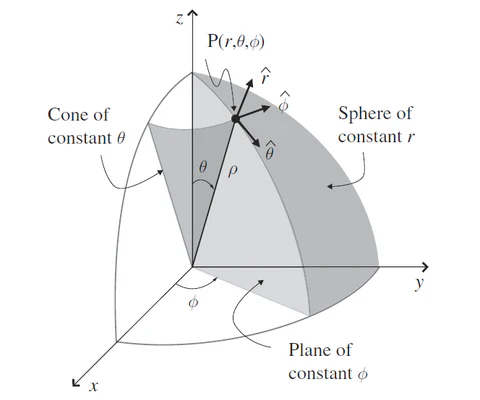
\includegraphics[width=8cm]{Figuras/Lineas-coordenadas-esfericas.png}
    \caption{Sistema coordenado esférico. Se puede apreciar que un punto en este es completamente determinado por la intersección de un ($\phi = $ constante), una superficie cónica ($\theta = $ constante) y una superficie esférica ($r = $ constante). Además, es posible apreciar la dirección de los tres vectores unitarios, $\hat{e}_r = \hat{r}$, $\hat{e}_\theta = \hat{\theta}$ y $\hat{e}_\phi = \hat{\phi}$.}
\end{figure}

\section{El operador Nabla}

Existen algunas operaciones diferenciales que puedes ser desarrolladas en campos escalares y vectoriales, y tienen una variedad de aplicaciones en física. Las tres más importantes corresponden al \emph{gradiente} de un campo escalar, la \emph{divergencia} de un campo vectorial, y el \emph{rotacional} de un campo vectorial.

Definiremos estas operaciones desde el punto de vista matemático, pues si bien pueden obtenerse a partir de nociones físicas y geométricas, en honor al tiempo no será posible hacer esta revisión. Para más detalles de estas, puede ver el capítulo 11 de Riley \cite{Riley}, o el capítulo 5 de Barea \cite{Barea}.

\begin{defi}
    Se define el operador \textbf{nabla} (o \emph{del} en inglés) en coordenadas cartesianas como 
    \begin{equation}
        \nabla \equiv \hat{\imath} \frac{\partial}{\partial x} + \hat{\jmath} \frac{\partial}{\partial y} + \hat{k} \frac{\partial}{\partial z} \ .
    \end{equation}
\end{defi}

\subsection{Gradiente}

\begin{defi}
    El \textbf{gradiente de un campo escalar}, $\nabla \phi \equiv \operatorname{grad}\phi$, corresponde a la operación que entrega como resultado la dirección \emph{de mayor cambio} en el campo $\phi$.

    En el caso que el campo sea constante (como un plano), entonces el gradiente corresponde al vector \emph{perpendicular} a la superficie definida por el campo $\phi$. 
\end{defi}

\begin{figure}[htbp]
    \centering
    
\includegraphics[width=12cm]{Figuras/Gradiente.png}
    \caption{Ilustración del concepto de gradiente. Nuestro campo escalar es representado por la escala de grises, donde un color más oscuro denota un mayor valor. Las flechas indican la dirección del gradiente en cada punto donde ellas aparecen, el que siempre apunta en la dirección de mayor cambio en la intensidad de la escala.}
\end{figure}

En coordenadas cartesianas, el gradiente puede escribirse como 
\begin{equation}
    \nabla \phi = \hat{\imath} \frac{\partial \phi}{\partial x} + \hat{\jmath} \frac{\partial \phi}{\partial y} + \hat{z} \frac{\partial \phi}{\partial z} \ ,
\end{equation}
mientras que en un sistema curvilíneo ortogonal podrá representarse como 
\begin{equation}
    \nabla \psi = \hat{e}_1 \frac{1}{h_1} \frac{\partial \psi}{\partial q_1} + \hat{e}_2 \frac{1}{h_2} \frac{\partial \psi}{\partial q_2} + \hat{e}_3 \frac{1}{h_3} \frac{\partial \psi}{\partial q_3} \ .
\end{equation}

Podemos representar cambios infinitesimales en el campo $\phi$, por ejemplo entre dos puntos $Q = (x_Q, y_Q, z_Q)$ y $P = (x_P, y_P, z_P)$ infinitesimalmente cercanos, mediante el diferencial $d\phi$:
\begin{equation*}
    d\phi = \phi(Q) - \phi(P) = \phi(x_Q, y_Q, z_Q) - \phi(x_P, y_P, z_P) = \frac{\partial \phi}{\partial x} dx + \frac{\partial \phi}{\partial y} dy + \frac{\partial \phi}{\partial z} dz \ ,
\end{equation*}
donde $d\x = (dx, dy, dz) = (x_Q - x_P, y_Q - y_P, z_Q - z_P)$ representa un vector que conecta por puntos $P$ y $Q$.

Notemos que 
\begin{equation*}
    d\phi = \nabla \phi \cdot d\x \ ,
\end{equation*}
donde $\theta$ es el ángulo que forman los vectores $\nabla \phi$ y $d\x$. Integremos ambos lados de la igualdad a lo largo de una curva que una los puntos $P$ y $Q$. Para el lado izquierdo, tenemos que
\begin{equation*}
    \int_P^Q d\phi = \phi(x_Q, y_Q, z_Q) - \phi(x_P, y_P, z_P) \ ,
\end{equation*}
por lo que en la igualdad resultará en 
\begin{equation}
    \int_P^Q d\phi = \int_C \nabla \phi \cdot d\x = \phi(x_Q, y_Q, z_Q) - \phi(x_P, y_P, z_P) \ ,
\end{equation}
de modo que la segunda integral, que es una integral de línea, \emph{no depende del camino seguido, sino únicamente de los puntos de inicio y término}.

\begin{defi}
    Decimos que un campo vectorial es \textbf{conservativo} si la integral de línea entre los puntos $A$ y $B$ es independiente del camino escogido entre ambas.
\end{defi}

Por ello, el gradiente de un campo escalar es un campo vectorial conservativo.

\subsection{Divergencia}

\begin{defi}
    Se define la \textbf{divergencia de un campo vectorial}, $\nabla \cdot \vec{A} = \operatorname{div} \vec{A}$ como una medida del flujo neto del campo $\vec{A}$ a través de una superficie cerrada.
\end{defi}

En coordenadas cartesianas, la divergencia viene dada por
\begin{equation}
    \nabla \cdot \vec{A} = \frac{\partial A_x}{\partial x} + \frac{\partial A_y}{\partial y} + \frac{\partial A_z}{\partial z} \ ,
\end{equation}
mientras que en coordenadas curvilíneas ortogonales puede representarse como 
\begin{equation}
    \nabla \cdot \vec{A} = \frac{1}{h_1 h_2 h_3} \left( \frac{\partial(h_2 h_3 C_1)}{\partial q_1} + \frac{\partial(h_1 h_3 C_2)}{\partial q_2} + \frac{\partial(h_1 h_2 C_3)}{\partial q_3} \right) \ ,
\end{equation}
donde en el sistema coordenado, $\vec{A} = (A_1, A_2, A_3)$.

Siguiendo la interpretación de la divergencia como un flujo, tendremos que si $\nabla \cdot \vec{A} > 0$, diremos que existe una \textbf{fuente} de líneas de campo en dicha región. En cambio, cuando $\nabla \cdot \vec{A} < 0$, diremos que existe un \textbf{sumidero} en la región.

\begin{figure}[htbp]
    \centering
    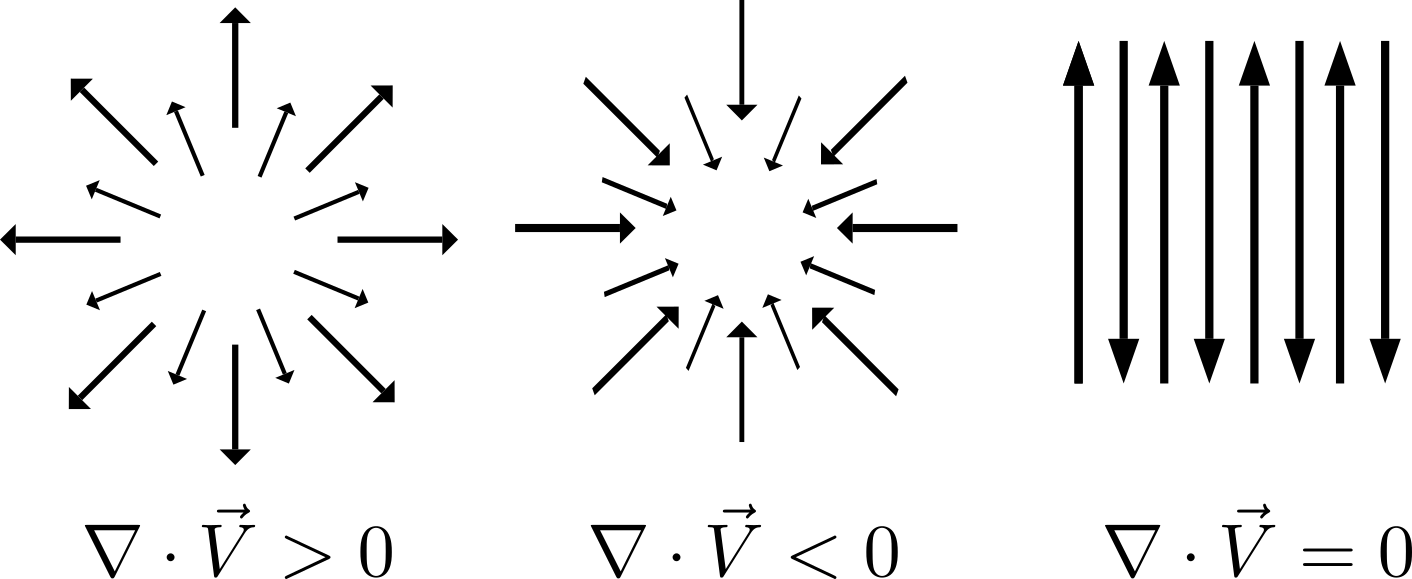
\includegraphics[width=8cm]{Figuras/Divergence.png}
    \caption{Divergencia de tres campos vectoriales. Nótese que el signo de esta cantidad depende del número de vectores \emph{entrantes} y \emph{salientes} de una superficie imaginaria que encierre al campo.}
\end{figure}

\begin{defi}
    Dado un campo vectorial $\vec{A}(\x)$, decimos que este es \textbf{solenoidal} si 
    \begin{equation}
        \nabla \cdot \vec{A} = 0 \ .
    \end{equation}
\end{defi}

\begin{ejemplo}
    La divergencia del vector posición puede obtenerse fácilmente en coordenadas cartesianas, de modo que 
    \begin{equation}
        \nabla \cdot \x = \frac{\partial x}{\partial x} + \frac{\partial y}{\partial y} + \frac{\partial z}{\partial z} = 3 \ .
    \end{equation}

    Dado que la divergencia de un vector es un escalar, este resultado es válido \textbf{para cualquier sistema de coordenadas}.
\end{ejemplo}

% \subsection{Teorema de Gauss, o de la divergencia}

Relacionado a la divergencia de un campo vectorial, existe un teorema que nos permite establecer una equivalencia entre integrales de superficie sobre una superficie $S$ cerrada, y una integral de volumen sobre la región $V$ encerrada por $S$.

\begin{teorema}{\textbf{(Teorema de la divergencia, o de Gauss).}} \marginnote{Teorema de Gauss}
    Dado un campo vectorial $\vec{A}(\x)$, continuo y diferenciable, la integral de su divergencia sobre una región $V$ es igual a la integral de superficie de la componente normal de $\vec{A}(\x)$ sobre la superficie $S$ que encierra a la región $V$:
    \begin{equation}
        \oint_S \vec{A}(\x) \cdot d\vec{S} = \int_V \nabla \cdot \vec{A}(\x) \, dV \ .
    \end{equation}
\end{teorema}

\begin{ejemplo}
    Siguiendo con el resultado obtenido en el ejemplo anterior, podemos utilizar el teorema de Gauss para una región $R$ arbitraria encerrada por una superficie $S$, gracias a lo cual obtenemos que 
    \begin{equation*}
        \oint_S \x \cdot d\vec{S} = \int_R \nabla \cdot \x \, dV = \int_R 3 \, dV = 3V \,
    \end{equation*}
    donde $V$ es el volumen de la región $R$. Reordenando términos, podemos concluir que el volumen de esta región se puede obtener como 
    \begin{equation}
        V = \frac{1}{3} \oint_S \x \cdot d\vec{S} \ .
    \end{equation}
\end{ejemplo}

\subsection{Rotacional}

\begin{defi}
    El \textbf{rotacional de un campo vectorial}, $\nabla \times \vec{A} = \operatorname{rot} \vec{A} = \operatorname{curl} \vec{A}$, correesponde a una medida de la \emph{densidad de circulación} de $\vec{A}$ alrededor de una curva $C$, que encierra una superficie $S$.

    De forma más coloquial, el rotacional mide la \emph{tendencia del campo a inducir una rotación alrededor de un punto} $\x$.
\end{defi}

En coordenadas cartesianas, este toma la forma 
\begin{align}
    \nonumber \nabla \times \vec{A} & = \left( \frac{\partial A_z}{\partial y} - \frac{\partial A_y}{\partial z} \right) \hat{\imath} + \left( \frac{\partial A_x}{\partial z} - \frac{\partial A_z}{\partial x} \right) \hat{\jmath} + \left( \frac{\partial A_y}{\partial x} - \frac{\partial A_x}{\partial y} \right) \hat{k} \\
    & = \left|
    \begin{array}{ccc}
        \hat{\imath} & \hat{\jmath} & \hat{k} \\
        \dfrac{\partial}{\partial x} & \dfrac{\partial}{\partial y} & \dfrac{\partial}{\partial z} \\
        A_x & A_y & A_z \\
    \end{array}
    \right| \ ,
\end{align}
o en coordenadas curvilíneas generalizadas,
\begin{equation}
    \nabla \times \vec{A} = \frac{1}{h_1 h_2 h_3} \left| 
    \begin{array}{ccc}
        h_1 \hat{e_1} & h_2 \hat{e}_2 & h_3 \hat{e}_3 \\
        \dfrac{\partial}{\partial q_1} & \dfrac{\partial}{\partial q_2} & \dfrac{\partial}{\partial q_3} \\
        h_1 A_1 & h_2 A_2 & h_3 A_3 \\
    \end{array}
    \right| \ .
\end{equation}

\begin{defi}
    Dado un campo vectorial $\vec{A}(\x)$, decimos que este es \textbf{irrotacional} si 
    \begin{equation}
        \nabla \times \vec{A} = 0 \ .
    \end{equation}
\end{defi}

% \subsection{Teorema de Stokes, o del rotacional}

De forma similar al teorema de Gauss, el teorema de Stokes es una forma de conectar una integral de línea de un campo $\vec{V}(\x)$ a lo largo de una curva cerrada $C$ con la integral de superficie del rotacional de $\vec{A}(\x)$ sobre la superficie $S$ encerrada por $C$.

\begin{teorema}{\textbf{(de Stokes, o del rotacional).}} \marginnote{Teorema de Stokes}
    Consideremos un campo vectorial $\vec{A}(\x)$ continuo y diferenciable. Entonces, la integral de línea alrededor de una curva cerrada $C$ es igual a la integral de superficie de la componente normal de su rotacional sobre cualquier superficie $S$ limitada por la curva $C$:
    \begin{equation}
        \oint_C \vec{A}(\x) \cdot d\x =  \int_S \left( \nabla \times \vec{A}(\x) \right) \cdot \, d\vec{S} \ .
    \end{equation}
\end{teorema}

\begin{figure}[htbp]
    \centering
    \begin{subfigure}[b]{0.45\textwidth}
        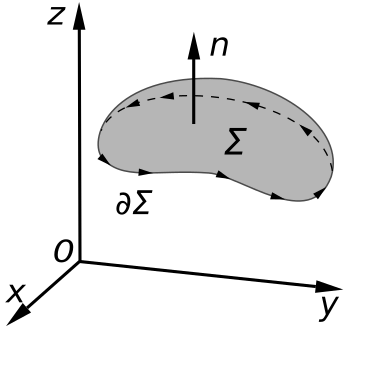
\includegraphics[width = 0.9\textwidth]{Figuras/Stokes'_Theorem.png}
        \caption{}
        \label{fig:stokes}
    \end{subfigure}
    \hfill
    \begin{subfigure}[b]{0.45\textwidth}
        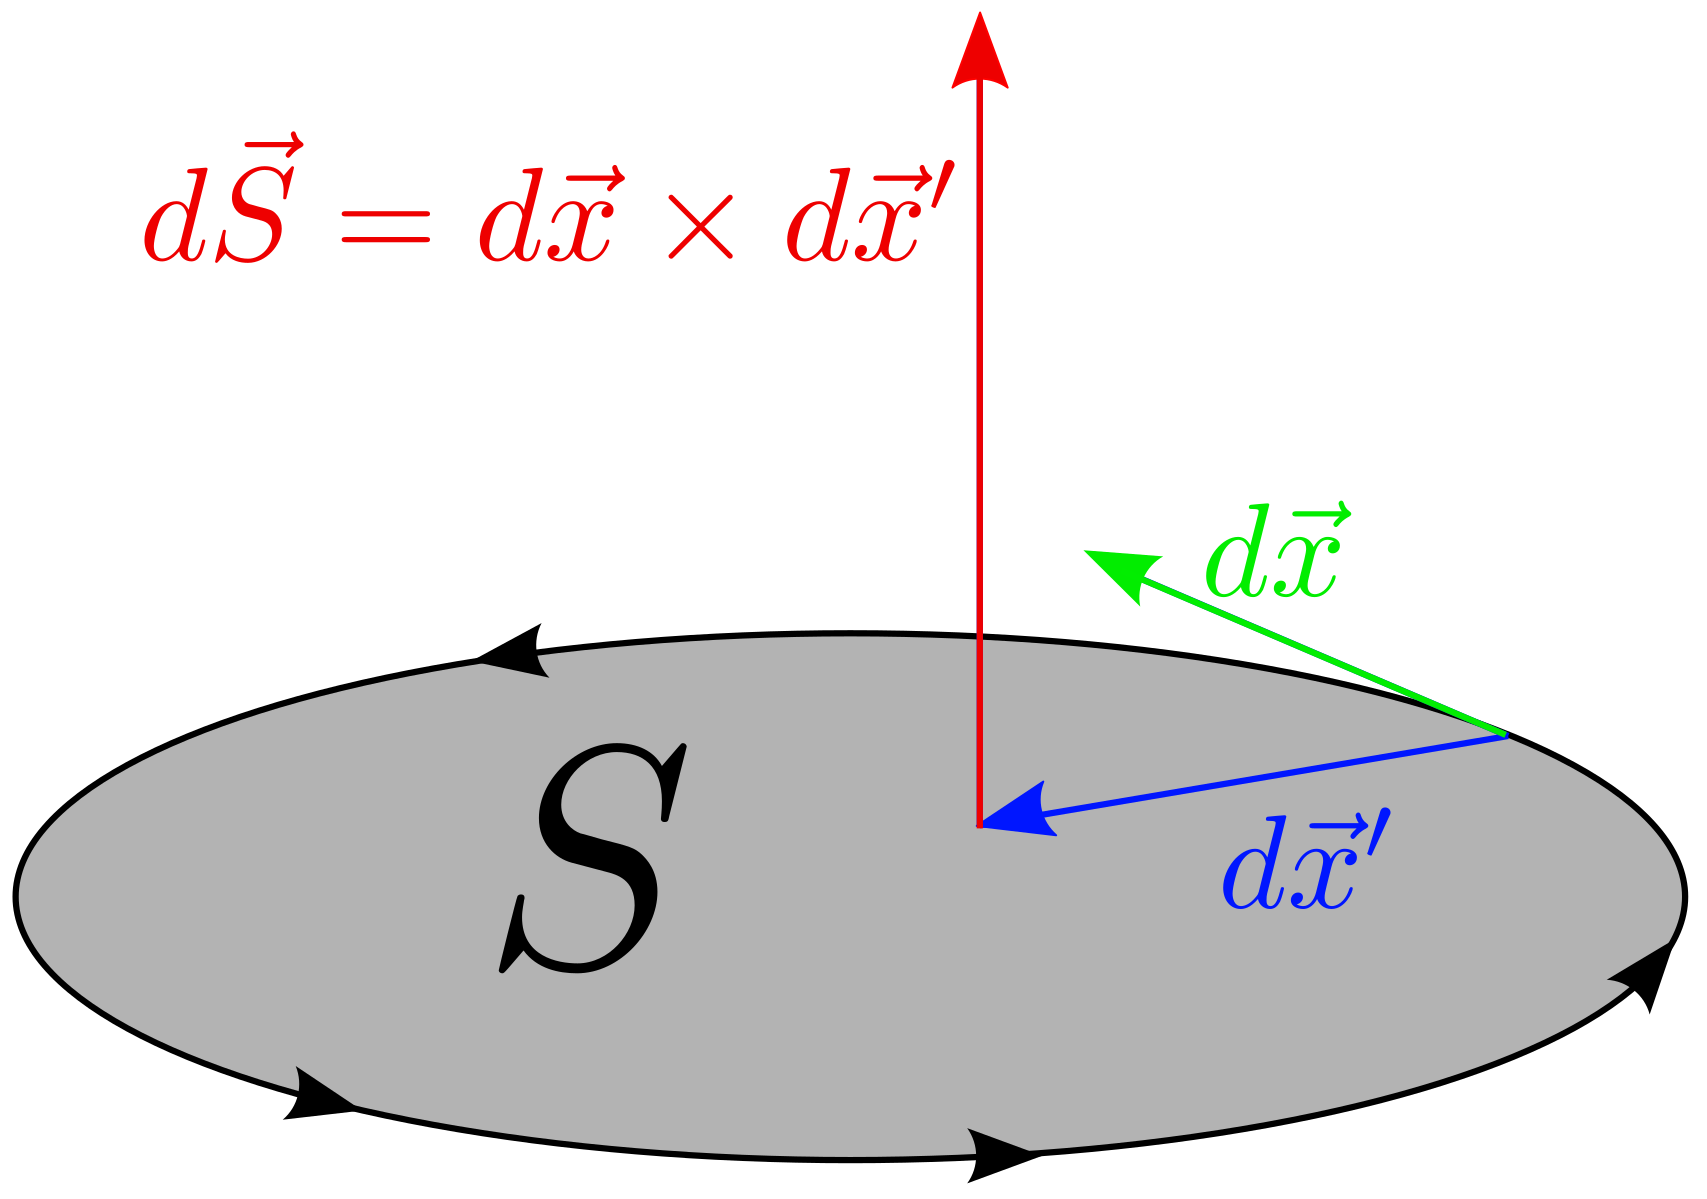
\includegraphics[width = 0.9\textwidth]{Figuras/Curlorient.png}
        % \vfill
        \caption{}
        \label{fig:orientation}
    \end{subfigure}
    % 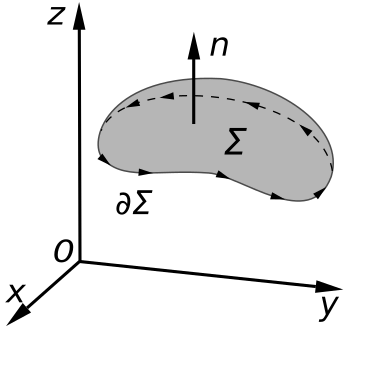
\includegraphics[width=8cm]{Figuras/Stokes'_Theorem.png}
    \caption{(a) Ilustración del Teorema de Stokes. La superficie $\Sigma$ se encuentra delimitada por la curva $\partial \Sigma$. El sentido en el que se recorre la curva y el vector normal a la superficie se encuentran relacionados entre sí mediante la regla de la mano derecha. (b) Una forma alternativa de representar la obtención del vector normal $d\vec{S}$ mediante el uso de un vector perpendicular a la superficie, $d\vec{x}'$.}
\end{figure}

En este caso, los diferenciales $d\x$ y $d\vec{S}$ están relacionados entre sí. Una vez fijamos el sentido en que recorreremos el contorno utilizando el vector $d\x$, el vector $d\vec{S}$ deberá seguir el sentido establecido por la \textbf{regla de la mano derecha}.

\begin{ejemplo}
    Considere el campo vectorial $\vec{F} = z\hat{\imath} + 2xy \hat{\jmath} + (x+y)\hat{k}$. Calcule la integral de superficie del rotacional de $\vec{F}$ sobre la superficie de la figura inferior.
    % \begin{figure}
    \begin{center}
        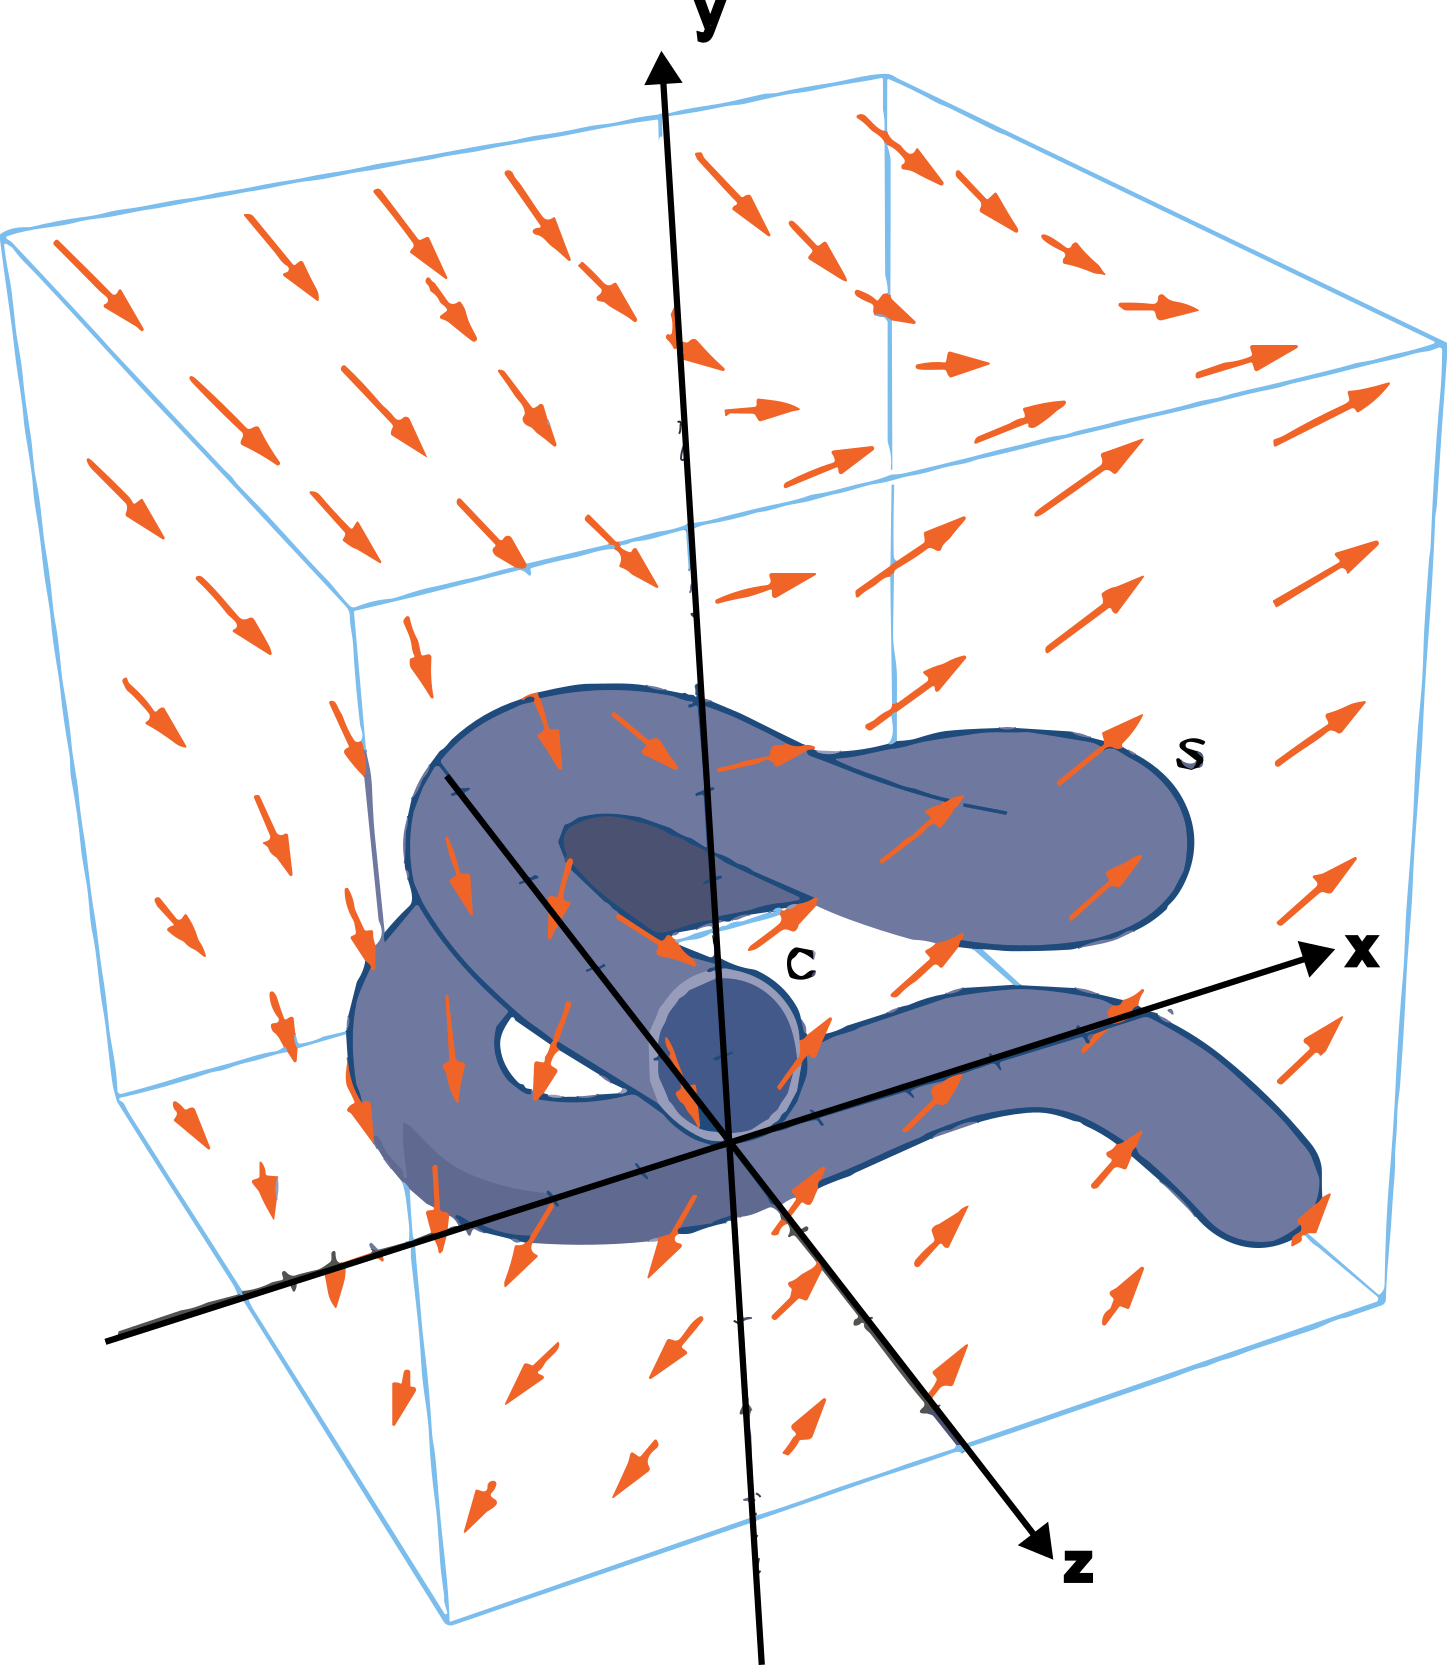
\includegraphics[width=6cm]{Figuras/superficie-complicada-2.png}
    \end{center}
    \captionof{figure}{Superficie complicada en presencia del campo vectorial $\vec{F}$.}
    % \end{figure}

    \textbf{Solución.}

    Lograr parametrizar esta superficie no es tarea sencilla, pues tampoco tenemos su forma funcional. Sin embargo, podemos hacer uso del Teorema de Stokes para solucionar dicha integral.

    Notemos que la superficie es cerrada, y su único contorno es un círculo, $C$, de radio 1 en el plano $xy$. Esta curva puede ser entonces parametrizada como $(\cos t, \sin t, 1)$, con $0 \leq t \leq 2\pi$. De esta forma, tenemos que 
    \begin{align*}
        \int_S (\nabla \times \vec{F}) \cdot d\vec{S} & = \int_C \vec{F} \cdot d\vec{r} \\
        & = \int_0^{2\pi} (1, 2 \sin t \cos t, \cos t + \sin t) \cdot (-\sin t, \cos t, 0) \, dt \\
        & = \int_0^{2\pi} (-\sin t + 2 \sin t \cos^2 t) \, dt \\
        & = \left[ \cos t - \frac{2\cos^3 t}{3} \right]_0^{2\pi} \\
        & = \cos(2\pi) - \frac{2 \cos^3 (2\pi)}{3} - \left( \cos 0 - \frac{2 \cos^3 0}{3} \right) \\
        & = 0 \ ,
    \end{align*}
    resultado que es independiente de la orientación de nuestro sistema coordenado.
\end{ejemplo}

Como vimos en el ejemplo anterior, a pesar de lo complicada que pueda ser una superficie, gracias al teorema de Stokes podemos simplificar los cálculos algebraicos. Es más, para \emph{cualquier} superficie suave $S$, delimitada por una curva $C$ cerrada, entonces 
\begin{equation*}
    \int_S (\nabla \times \vec{F}) \cdot d\vec{S} = 0 \ ,
\end{equation*}
debido a que la integral de línea sobre el contorno de una superficie suave se anulará.

\subsection{Identidades vectoriales}

Dados los campos escalares $\phi$ y $\psi$, y los campos vectoriales $\vec{A}$ y $\vec{B}$, algunas identidades que surgen de la aplicación del operador nabla sobre sumas o productos de estos campos son las siguientes:
\begin{itemize}
    \item $\nabla (\phi + \psi) = \nabla \phi + \nabla \psi$.
    \item $\nabla \cdot \left( \vec{A} + \vec{B} \right) = \nabla \cdot \vec{A} + \nabla \cdot \vec{B}$.
    \item $\nabla \times \left( \vec{A} + \vec{B} \right) = \nabla \times \vec{A} + \nabla \times \vec{B}$.
    \item $\nabla(\phi \psi) = \phi \nabla \psi + \psi \nabla \phi$.
    \item $\nabla \cdot \left( \phi \vec{A} \right) = \phi \nabla \cdot \vec{A} + \vec{A} \cdot \nabla \phi$.
    \item $\nabla \cdot (\vec{A} \times \vec{B}) = \vec{B} \cdot (\nabla \times \vec{A}) - \vec{A} \cdot (\nabla \times \vec{B})$.
    \item $\nabla \times (\phi \vec{A}) = \nabla \phi \times \vec{A} + \phi \nabla \times \vec{A}$.
    \item $\nabla(\vec{A} \cdot \vec{B}) = \vec{A} \times (\nabla \times \vec{B}) + \vec{B} \times (\nabla \times \vec{A}) + (\vec{A} \cdot \nabla) \vec{B} + (\vec{B} \cdot \nabla) \vec{A}$,
    donde 
    \begin{equation*}
        \vec{A} \cdot \nabla = A_x \frac{\partial}{\partial x} + A_y \frac{\partial}{\partial y} + A_z \frac{\partial}{\partial z} \ .
    \end{equation*}
\end{itemize}


De igual forma, podemos estudiar las aplicaciones sucesivas del operador nabla sobre campos escalares o vectoriales. Enumeraremos únicamente aquellas cantidades que sí tiene sentido definir:
\begin{itemize}
    \item \textbf{Divergencia de un gradiente}, $\nabla \cdot (\nabla \phi) = (\nabla \cdot \nabla) \phi = \nabla^2 \phi$, operación que es conocida como \textbf{laplaciano} de un campo escalar. En coordenadas curvilíneas ortogonales,
    \begin{equation}
        \nabla^2 \phi = \frac{1}{h_1 h_2 h_3}\left[ \frac{\partial}{\partial q_1} \left( \frac{h_2 h_3}{h_1} \frac{\partial \phi}{\partial q_1} \right) + \frac{\partial}{\partial q_2} \left( \frac{h_1 h_3}{h_2} \frac{\partial \phi}{\partial q_2} \right) + \frac{\partial}{\partial q_3} \left( \frac{h_1 h_2}{h_3} \frac{\partial \phi}{\partial q_3} \right) \right] \ .
    \end{equation}
    \item \textbf{Rotacional de un gradiente}, $\nabla \times (\nabla \phi) = 0$, pues las derivadas parciales cruzadas que surgirán se cancelarán entre sí. En consecuencia, todo gradiente es irrotacional.
    \item \textbf{Gradiente de una divergencia}, $\nabla (\nabla \cdot \vec{A})$.
    \item \textbf{Divergencia de un rotacional}, $\nabla \cdot (\nabla \times \vec{A}) = 0$, donde nuevamente las derivadas parciales cruzadas se anularán. En consecuencia, todo rotacional es solenoidal.
    \item \textbf{Rotacional de un rotacional}, $\nabla \times (\nabla \times \vec{A}) = \nabla (\nabla \cdot \vec{A}) - \nabla^2 \vec{A}$.
\end{itemize}

% \section{Teoremas integrales}


\section{Teoría del potencial}

Cerramos este capítulo explicando la importancia de los resultados aquí descritos. Consideremos un campo escalar $\phi(\x)$. Al calcular su gradiente, obtenemos un campo vectorial, que llamaremos $\vec{F}(\x) = \nabla \phi(\x)$. De aquí, podemos inferir dos resultados:
\begin{enumerate}
    \item El campo vectorial resultante es irrotacional, pues $\nabla \times \vec{F} = \nabla \times (\nabla \phi) = 0$.
    \item Por definición, $\vec{F} \cdot d\x = \nabla \phi \cdot d\x = d\phi$, de modo que para cualquier curva cerrada, $\oint_C \vec{F} \cdot d\x = \oint_C d\phi = 0$.
\end{enumerate}

Del segundo resultado, podemos concluir que \emph{la integral de línea de} $\vec{F}$ \emph{a lo largo de cualquier trayectoria que una los puntos} $A$ y $B$ \emph{proporciona siempre el mismo valor, y es independiente de la trayectoria escogida}. Nos referiremos a este comportamiento diciendo que el campo $\vec{F}(\x)$ es \textbf{conservativo}.

\begin{teorema}
    Dado un campo vectorial $\vec{F}(\x)$, son equivalentes las tres afirmaciones:
    \begin{itemize}
        \item $\vec{F}(\x)$ es un campo conservativo.
        \item $\vec{F}(\x)$ es irrotacional.
        \item Existe un campo escalar $\phi$, denominado \textbf{potencial escalar}, tal que $\vec{F}(\x) = - \nabla \phi$.
    \end{itemize}
\end{teorema}

Ejemplos del resultado de este teorema son:
\begin{itemize}
    \item El campo eléctrico, $\vec{E}$, que se puede definir a partir de un potencial electrostático $\phi$, tal que $\vec{E} = - \nabla \phi$.
    \item Toda fuerza $\vec{F}$, que se encuentre asociada a una energía potencial $U$, tal que $\vec{F} = - \nabla U$. Algunas de ellas son la fuerza elástica, la fuerza gravitacional o la fuerza eléctrica.
\end{itemize}

\subsection{Teorema de Helmholtz}

Bajo ciertas condiciones, el resultado obtenido anteriormente no será suficiente. En dichas condiciones, es posible definir una construcción más complicada utilizando el siguiente teorema.

\begin{teorema}{\textbf{(de Helmholtz).}}
    Sea $\vec{V}(\x)$ un campo vectorial diferenciable, con derivadas parciales continuas, y cuya divergencia y rotacional se anulan en el límite $|\x| \to \infty$. Entonces, podemos descomponer $\vec{V}$ en una componente \emph{irrotacional}, y en una componente \emph{solenoidal}, dependientes de un \textbf{potencial escalar} $\phi$ y un \textbf{potencial vectorial} $\vec{A}$, respectivamente:
    \begin{equation}
        \vec{V} = -\nabla \phi + \nabla \times \vec{A} \ ,
    \end{equation}
    donde
    \begin{align}
        \phi(\x)    & = \frac{1}{4\pi} \int_V \frac{\nabla \cdot \vec{V}(\x')}{|\x-\x'|} \, dV' \ , \\
        \vec{A}(\x) & = \frac{1}{4\pi} \int_V \frac{\nabla \times \vec{V}(\x')}{|\x-\x'|} \, dV' \ . 
    \end{align}
\end{teorema}

\begin{corolario}
    Un campo vectorial $\vec{J}(\x)$ solenoidal, puede representarse en términos de un potencial vector $\vec{A}$, tal que 
    \begin{equation}
        \vec{J}(\x) = \nabla \times \vec{A} \ .
    \end{equation}
\end{corolario}
\chapter[Introducción a los Tensores Cartesianos]{Introducción a los\breaktitle Tensores Cartesianos}

% Llegando al último capítulo del curso, nos desviamos un poco de la noción de que este curso se dedica a enseñar métodos matemáticos que pueden ser útiles en Física, para en su lugar introducir cantidades y conceptos con la misma utilidad.

Una de las nociones más importantes que tenemos en física clásica es el hecho de que \emph{los fenómenos físicos son los mismos, y no deben cambiar según el observador}, más allá de que las componentes de las cantidades que los describen puedan hacerlo. Particularmente, nos centraremos en las \emph{transformaciones ortogonales} de un sistema coordenado, referidas de forma más común como \textbf{rotaciones}. 

Por ejemplo, un vector que describe la posición de un objeto en función del tiempo puede ser diferente según el sistema de coordenadas en que se lo describa, pero el movimiento \emph{físico} del objeto seguirá siendo el mismo.

% \section{Sistemas Coordenados}

% Antes de entrar más de lleno en la discusión, recordemos e introduzcamos algunas definiciones.

% \begin{defi} \marginnote{Delta de Kronecker}
%     Se denomina \textbf{delta de Kronecker} al elemento $\delta_{ij}$, definido en un espacio vectorial de $n$ dimensiones como
%     \begin{equation}
%         \delta_{ij} = \begin{dcases}
%             1, \qquad i = j \\
%             0, \qquad i \neq j
%         \end{dcases} \ .
%     \end{equation} 

%     Este elemento puede representarse de forma matricial como la matriz identidad del espacio de dimensión $n$.
% \end{defi}

% \newpage

% \begin{defi} \marginnote{Base ortonormal}
%     Sea un conjunto de vectores unitarios $\left\{ \hat{e}_i\right\}_{i=1}^n$ de un espacio $n$-dimensional. Diremos que este forma una \textbf{base ortonormal} si al realizar el producto escalar entre elementos del conjunto, se cumple la relación
%     \begin{equation}
%         \hat{e}_i\cdot \hat{e}_j = \delta_{ij} \ ,
%     \end{equation}
%     donde $\delta_{ij}$ es la delta de Kronecker.
% \end{defi}

% \begin{defi} \marginnote{Vector posición}
%     Dado un sistema coordenado en un espacio de $n$ dimensiones, podemos definir el \textbf{vector posición} $\vec{x}$, que une el origen del sistema con punto con coordenadas $x_i$, con $i = 1, 2, \dots, n$ como
% \begin{equation} \label{eq:vector-posicion}
%     \vec{x} = \sum_{i=1}^n x_i \hat{e}_i \ ,
% \end{equation}
% donde las \textbf{componentes del vector} en la base $\{ \hat{e}_i\}_{i=1}^n$ pueden expresarse como
% \begin{equation}
%     x_i = \vec{x} \cdot \hat{e}_i \ .
% \end{equation}
% \end{defi}

% Más allá de que el vector posición es aquel que tiene un sentido \emph{físico} a partir del cual hacer las definiciones, podemos descomponer \emph{cualquier vector} en la base $\{ \hat{e}_i\}_{i=1}^n$ en términos de sus respectivas componentes, sin importar la cantidad que este pueda representar.


\section{Transformaciones Ortogonales}

Cuando estamos trabajando con coordenadas cartesianas, podemos definir un nuevo sistema coordenado, que llamaremos $x'_i$ y cuya base es $\{ \hat{e}_i'\}_{i=1}^n$, que corresponde a una \emph{rotación} del sistema $x_i$ definido anteriormente, como se ve en la figura \ref{fig:bases-ortonormales}.

\begin{figure}[htbp]
    \centering
    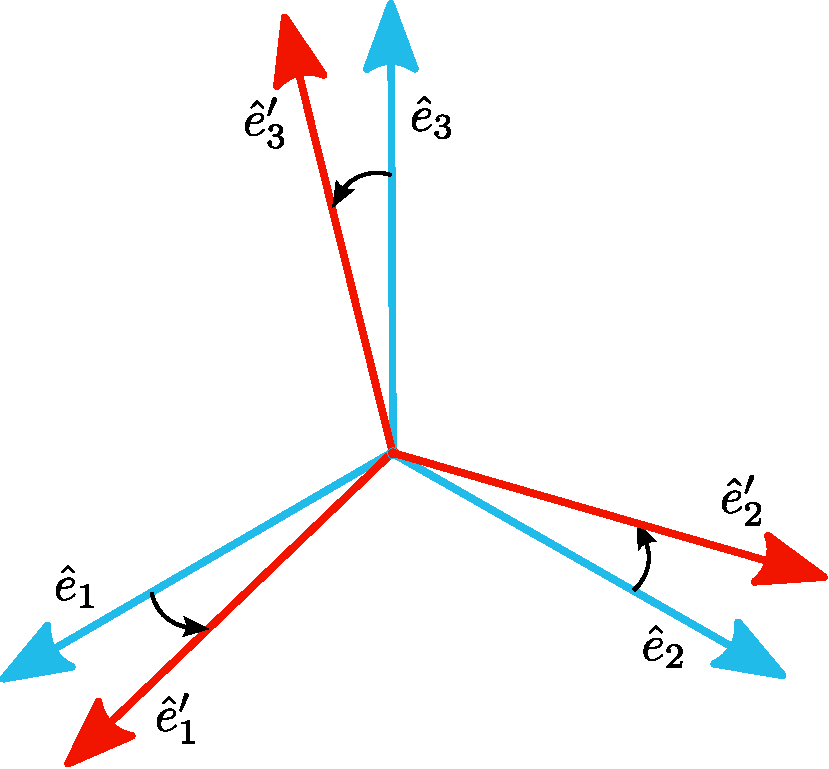
\includegraphics[width=6cm]{Figuras/fig-rotacion-bases.pdf}
    \caption{Una transformación ortogonal de dos bases ortonotmales en 3 dimensiones, $\hat{e}_i$ y $\hat{e}'_j$}
    \label{fig:bases-ortonormales}
\end{figure}

Respecto de esta nueva base, un vector $\vec{v}$ cualquiera puede ser descompuesto en sus componentes $v_i'$ \emph{en la base} $\{ \hat{e}_i'\}_{i=1}^n$,
\begin{equation}
    \vec{v} = \sum_{i=1}^n v_i' \hat{e}'_i \ .
\end{equation}

Dado que, si bien dan origen a sistemas de coordenadas diferentes, ambas bases se encuentran en el mismo espacio vectorial, ¿Cómo podemos relacionar ambas bases entre sí? Para ello, haremos uso de una \textbf{matriz de transformación}, definida como
\begin{equation}
    A = \begin{pmatrix}
        a_{11} & a_{12} & \dots & a_{1n} \\
        a_{21} & a_{22} & \dots & a_{2n} \\
        \vdots & \vdots & \ddots & \vdots \\
        a_{n1} & a_{n2} & \dots & a_{nn}
    \end{pmatrix} =
    \begin{pmatrix}
        \hat{e}_1 \cdot \hat{e}'_1 & \hat{e}_1 \cdot \hat{e}'_2 & \dots & \hat{e}_1 \cdot \hat{e}'_n \\
        \hat{e}_2 \cdot \hat{e}'_1 & \hat{e}_2 \cdot \hat{e}'_2 & \dots & \hat{e}_2 \cdot \hat{e}'_n \\
        \vdots & \vdots & \ddots & \vdots \\
        \hat{e}_n \cdot \hat{e}'_1 & \hat{e}_n \cdot \hat{e}'_2 & \dots & \hat{e}_n \cdot \hat{e}'_n
    \end{pmatrix} \ .
\end{equation}

De este modo, un vector de la base $\vec{e}'_i$ puede escribirse también en términos de la base $\vec{e}_i$,
\begin{equation} \label{eq:transformacion-coordenadas}
    \hat{e}'_i = \sum_{j=1}^n a_{ij} \hat{e}_j \ ,
\end{equation}
por lo que podemos reescribir el vector $\vec{v}$ como
\begin{equation} \label{eq:transformacion-vector}
    \vec{v} = \sum_{i=1}^n v'_i \left( \sum_{j=1}^n a_{ij} \hat{e}_j \right) \ .
\end{equation}

\subsection{Convenio de suma de Einstein}

Antes de continuar la discusión, es útil introducir el  \textbf{convenio de suma de Einstein}, que establece que en toda expresión donde se repitan dos índices iguales, \emph{existe una suma implícita sobre todo el rango de variación del índice}. Es más, el índice de suma \emph{es una etiqueta arbitraria}, por lo que puede ser renombrada a conveniencia.

Por ejemplo, las expresiones \eqref{eq:vector-posicion} y \eqref{eq:transformacion-vector} pueden reescribirse como
\begin{align}
    \vec{v} & = v_i \hat{e}_i \, , \\
    \vec{v} & = v'_i a_{ij} \hat{e}_j .
\end{align}

Además, dado que existe una suma implícita, podemos aplicar la delta de Kronecker para reemplazar índices en una multiplicación, de modo que
\begin{equation}
    a_{ij} b_{jk} \delta_{ki} = a_{ij} b_{ji} = a_{kj} b_{jk} \ .
\end{equation}


La discusión hecha hasta ahora es válida para cualquier transformación de coordenadas entre dos bases distintas. Para los efectos de este curso, nos interesa trabajar únicamente con \emph{transformaciones ortogonales}.

\begin{defi} \marginnote{Transformación ortogonal}
    Una \textbf{transformación ortogonal} es aquella transformación de cambio de base que permite convertir una base ortonormal $\{\hat{e}_i\}_{i=1}^n$ en una nueva base ortonormal $\{\hat{e}'_i\}_{i=1}^n$.
\end{defi}

Para asegurarnos que la transformación \eqref{eq:transformacion-coordenadas} sea una transformación ortogonal, debe además satisfacer que
\begin{align}
    \delta_{ij} & = \hat{e}'_i \cdot \hat{e}'_j \\
    & = \left( \sum_{k=1}^n a_{ik} \hat{e}_k \right) \left( \sum_{l=1}^n a_{jl} \hat{e}_l \right) \\
    & = \sum_{k=1}^n \sum_{l=1}^n a_{ik} a_{jl} (\hat{e}_k \cdot \hat{e}_l) \\
    & = \sum_{k=1}^n \sum_{l=1}^n a_{ik} a_{jl} \delta_{kl} \\
    & = \sum_{k=1}^n a_{ik} a_{jk} \ , \label{eq:delta-transformacion-ortogonal}
\end{align}
o bien, matricialmente,
\begin{equation}\label{eq:condicion-matricial}
    A \cdot (A^T) = I \ ,
\end{equation}
que al calcular el determinante, observamos que
\begin{equation}
    \det(A)^2 = 1 \ , 
\end{equation}
de modo que una transformación ortogonal deberá satisfacer que $\det(A) = 1$, caso en que se denomina \emph{transformación propia}, o bien que $\det(A) = -1$, lo que se conoce como \emph{transformación impropia}.

En particular, de \eqref{eq:condicion-matricial} podemos observar que para una transformación ortogonal, $A^T = A^{-1}$, es decir, la transpuesta de la transformación coincide con su inversa, de modo que también se satisface que
\begin{equation}
    (A^T) \cdot A = I \ ,
\end{equation}
o en notación indicial,
\begin{equation}
    \sum_{k=1}^n a_{ki} a_{kj} =  \delta_{ij} \ .
\end{equation}

\section{Tensores Cartesianos}

Hasta ahora, hemos discutido las propiedades de los vectores, elementos con los que ya somos familiares. Sin embargo, seguimos sin responder la incógnita de \emph{¿qué es un tensor?}. Para ello, introduzcamos una operación entre vectores.

\begin{defi}\marginnote{Producto externo}
    Dados dos vectores $\vec{u} = u_i \hat{e}_i$ y $\vec{v} = v_i \hat{e}_i$, se define el \textbf{producto externo} entre ambos vectores como la cantidad
    \begin{equation}
        T_{ij} = u_i v_j \ .
    \end{equation}
\end{defi}

Como podemos ver de la definición anterior, necesitamos de \emph{dos índices} para definir el producto externo. ¿Qué ocurre con esta cantidad si, en lugar de utilizar la base $\hat{e}_i$, utilizamos la base $\hat{e}'_i$? En otras palabras, ¿cómo transforma $T_{ij}$ bajo transformaciones ortogonales? Notamos que
\begin{equation}
    T'_{ij} = u'_i v'_j = (a_{ik}u_k)(a_{jl} v_l) = a_{ik} a_{jl} (u_k v_l) =  a_{ik} a_{jl} T_{kl} \ .
\end{equation}

Observamos pues, que $T_{ij}$ transforma de manera similar a los vectores bajo transformaciones ortogonales. A cantidades que siguen una regla de transformación de este tipo, las llamamos \emph{tensores (cartesianos) de rango 2}, pues requerimos de dos matrices de transformación para definirlas adecuadamente. Observamos que, para un espacio de $n$ dimensiones, estos elementos tendrán $n^2$ componentes.

Esta noción puede ampliarse a más dimensiones, según la siguiente definición,
\begin{defi} \marginnote{Tensor cartesiano}
    Dado un espacio de $n$ dimensiones, el conjunto de $n^r$ cantidades $T_{i_1 i_2 \dots i_r}$ definidas en cada sistema ortogonal de coordenadas, son las componentes de un \textbf{tensor cartesiano de rango} $\mathbf{r}$ si, bajo transformaciones ortogonales, sus valores siguien la regla de transformación
    \begin{equation}
        T'_{i_1 i_2 \dots, i_r} = a_{i_1 j_1} a_{i_2 j_2} \dots a_{i_r j_r} T_{j_1 j_2 \dots j_r} \ . 
    \end{equation}
\end{defi}

Gracias a esta definición, observamos que los \textbf{vectores}, que tienen una sola matriz de transformación en su definición \eqref{eq:transformacion-vector}, son \emph{tensores de rango 1}. A su vez, los \textbf{escalares} son cantidades que no se ven modificadas frente a una transformación de coordendas, de modo que $\rho' = \rho$. Por ello, podemos considerarlos \emph{tensores de rango 0}.

\begin{ejemplo}
    \textbf{Tensor de inercia.}

    Consideremos un cuerpo con densidad $\rho(x_i)$, contenido en una región $V$ que rota \emph{rígidamente} respecto de un eje con dirección $\hat{\omega}$ con velocidad angular $\omega$. Entonces, podemos hallar su momento angular respecto al origen del sistema (ubicado sobre el eje de rotación) como
    \begin{align*}
        \vec{L} & = \int_V \x \times d\vec{p} \\
        & = \int_V \rho(x) \x \times \vec{v} \ dV \\
        & = \int_V \rho(x) \x \times (\vec{\omega} \times \x) \ dV \ .
    \end{align*}
    Usando la identidad $\vec{A} \times (\vec{B} \times \vec{C}) = \vec{B} (\vec{A} \cdot \vec{C}) - \vec{C} (\vec{A} \cdot \vec{B})$, podemos escribir
    \begin{equation*}
        \vec{L} = \int_V \rho(x) [\vec{\omega}(\x \cdot \x) - \x (\vec{\omega} \cdot \x)] \ dV \ ,
    \end{equation*}
    o en términos de las componentes del vector,
    \begin{align*}
        L_i & = \int_V \rho(x) [\omega_i(x_k x_k) - x_i(\omega_j x_j)] \ dV \\
        & = \int_V \rho(x) [(\delta_{ij} \omega_j)(x_k x_k) - x_i(\omega_j x_j)] \ dV \\
        & = \left( \int_V \rho(x) [\delta_{ij} (x_k x_k) - x_i x_j] \ dV \right) \omega_j \ ,
    \end{align*}
    es decir, 
    \begin{equation*}
        L_i = I_{ij} \omega_j \, 
    \end{equation*}
    donde $I_{ij}$ es el \emph{tensor de inercia} definido como
    \begin{equation*}
        \int_V \rho(x) [\delta_{ij} (x_k x_k) - x_i x_j] \ dV \ .
    \end{equation*}

    ¿Es esta cantidad efectivamente un tensor cartesiano? Revisemos cómo transforma bajo una transformación ortogonal,
    \begin{align*}
        I'_{ij} & = \int_V \rho'(x') [\delta_{ij} (x'_k x'_k) - x'_i x'_j] \ dV' \\
        & = \int_V \underbrace{\rho(x)}_{\text{Escalar}} [\delta_{ij}\underbrace{(x_k x_k)}_\text{Escalar} - (a_{il} x_l)(a_{jm} x_m)] \ dV \\
        & = \int_V \rho(x) [(a_{il}a_{jl})(x_k x_k) - (a_{il} x_l)(a_{jm} x_m)] \ dV \\
        & = \int_V \rho(x) [(a_{il}a_{jm}\delta_{lm})(x_k x_k) - (a_{il} x_l)(a_{jm} x_m)] \ dV \\
        & = (a_{il} a_{jm}) \int_V \rho(x) [(\delta_{lm})(x_k x_k) - x_l x_m] \ dV \\
        & = a_{il} a_{jm} I_{lm} \ ,
    \end{align*}
    de modo que efectivamente $I_{jl}$ transforma como un tensor cartesiano.
\end{ejemplo}

\subsection{Propiedades}

En este contexto, vale la pena mencionar con algo más de detalle a dos propiedades.

\begin{propiedad}
    \textbf{Propiedades de los tensores cartesianos.}

    \begin{enumerate}
        \item Si \emph{todas las componentes de un tensor se anulan en un sistema coordenado ortogonal}, ellas se anularán \emph{en todo sistema coordenado ortogonal}.  Esta propiedad nos interesa, ya que nos indica que la anulación de un tensor \textbf{es una propiedad intrínseca} de este. De esta propiedad surge la importancia de utilizar tensores en Física, pues nos permite plantear leyes \emph{que no dependen del sistema coordenado en que trabajamos}, sino únicamente del fenómeno estudiado.
        
        Por ejemplo, podemos estar estudiando el momento de inercia de un cuerpo en movimiento, el cual es un tensor de rango 2. Si diera la casualidad de que este es cero en algún sistema coordenado ortogonal, esto quiere decir que, \textbf{en cualquier sistema coordenado ortogonal}, el cuerpo \emph{no se encuentra rotando}.
    
        \item Existen algunos \textbf{tensores invariantes} o \textbf{isotrópicos}, los cuales tienen siempre las mismas componentes \emph{en cualquier sistema coordenado}. Un ejemplo de estos es la delta de Kronecker, pues en cualquier sistema coordenado tendrá las mismas componentes, 1 si $i=j$ y 0 si $i\neq j$.
        
        En efecto, podemos observar que la delta de Kronecker transforma como
        \begin{equation}
            \delta'_{ij} = a_{ik} a_{jl} \delta_{kl} = a_{ik} a_{jk} = \delta_{ij} \ .
        \end{equation}
    \end{enumerate}
\end{propiedad}



\section{Álgebra Tensorial}

Dicho rápido y sencillo, hemos visto que los tensores de rango 1 y rango 2 se comportan como vectores columna y como matrices, respectivamente. Por ello, esperaríamos que sea posible definir operaciones tensoriales similares a las definidas para estos elementos, incluyendo la posibilidad de construir tensores a partir de otros.

\begin{itemize}
    \item \textbf{Adición y sustracción.} Se define la adición (o suma) y sustracción (o resta) de dos tensores \emph{del mismo orden} componente a componente, es decir,
    \begin{align}
        S_{ij \dots k} & = V_{ij \dots k} + W_{ij \dots k} \ , \\
        D_{ij \dots k} & = V_{ij \dots k} - W_{ij \dots k} \ .
    \end{align}
    % \item \textbf{Producto por escalar.}
    \item \textbf{Permutación de índices.} La operación de permutar dos índices de un tensor de rango $r$, define un nuevo tensor de rango $r$. Es decir, dado un tensor $T_{ijk \dots l}$ de rango $r$, la cantidad
    \begin{equation}
        B_{ijk \dots l} = T_{ikj \dots l} 
    \end{equation}
    es también un tensor de rango $r$.

    \item \textbf{Producto tensorial, o directo.} De manera similar al \emph{producto externo} de dos vectores que calculamos anteriormente, podemos definir el producto entre dos tensores de diferente rango, digamos $r$ y $s$, lo que permite formar un nuevo vector de rango $r+s$,
    \begin{equation}
        C_{i_1 i_2 \dots i_{r+s}} = A_{i_1 i_2 \dots i_r} \cdot B_{i_{r+1} i_{r+2} \dots i_{r+s}} \ .
    \end{equation}
    
    En este caso, es relevante respetar la posición de los índices en el producto, pues en general el tensor $C_{ij} = A_i B_j$ será distinto al vector $D_{ij} = A_j B_i$, como consecuencia de la permutación de índices.

    Esta operación incluye, por supuesto, el producto entre un tensor de rango 0 (un escalar) y un tensor de rango $r$, definiendo el \emph{prodcuto por un escalar}.

    \item \textbf{Contracción de índices.} El producto escalar entre dos vectores nos entrega un escalar en lugar de un tensor de orden 2, como consecuencia de la repetición de índices en el producto. De manera similar, la repetición de dos índices dentro de un tensor de orden $r$ (digamos, el $s$-ésimo y el $t$-ésimo índice), es equivalente a un tensor de orden $r-2$,
    \begin{equation}
        B_{i_1 i_2 \dots i_{r-2}} = A_{i_1 i_2 \dots j \dots j \dots i_{r-2}} \ ,
    \end{equation}
    o de forma equivalente,
    \begin{equation}
        B_{i_1 i_2 \dots} = A_{i_1 i_2 \dots i_r} \delta_{i_s i_t} \ .
    \end{equation}

    \item \textbf{Ley del cociente.} Consideremos el caso en que tenemos una expresión de la forma
    \begin{equation}\label{eq:ley-cociente}
        A_{pq \dots k \dots m} B_{ij \dots k \dots n} = C_{pq \dots m ij \dots n} \ ,
    \end{equation}
    donde sabemos que $B$ y $C$ son tensores de rango $r$ y $s$, respectivamente, pero desconocemos si $A$ es un tensor. La ley del cociente establece que \emph{si la relación \eqref{eq:ley-cociente} es válida en cualquier sistema de coordenadas, entonces} $A$ es un tensor de orden $s-r+2$. La demostración (para el caso $r=s=2$) puede ser hallada en el capítulo 26, sección 7 de Riley \cite{Riley}.
    
    \item \textbf{Simetría.} Cuando un tensor no cambia bajo la permutación de dos de sus índices, 
    \begin{equation}
        T_{i_1 i_2 \dots i_s \dots i_t \dots i_r} = T_{i_1 i_2 \dots i_t \dots i_s \dots i_r} \ , 
    \end{equation}
    se dice que este es \emph{simétrico} respecto a dichos índices. Si, en cambio,
    \begin{equation}
        T_{i_1 i_2 \dots i_s \dots i_t \dots i_r} = - T_{i_1 i_2 \dots i_t \dots i_s \dots i_r} \ ,
    \end{equation}
    decimos que el tensor es \emph{antisimétrico} respecto de dichos índices. En general, un tensor de rango $r$ puede escribirse como la suma de un tensor simétrico y un tensor antisimétrico respecto de la misma permutación de índices, de modo que
    \begin{align}
        T_{i_1 i_2 \dots i_s \dots i_t \dots i_r} & = \frac{1}{2} (T_{i_1 i_2 \dots i_s \dots i_t \dots i_r} + T_{i_1 i_2 \dots i_t \dots i_s \dots i_r}) + \frac{1}{2}(T_{i_1 i_2 \dots i_s \dots i_t \dots i_r} - T_{i_1 i_2 \dots i_t \dots i_s \dots i_r}) \\
        & = S_{i_1 i_2 \dots i_s \dots i_t \dots i_r} + A_{i_1 i_2 \dots i_s \dots i_t \dots i_r} \ .
    \end{align}

    En física, a veces es común utilizar la siguiente notación,
    \begin{align}
        T_{i_1 i_2 \dots (i_s| \dots |i_t) \dots i_r} & \equiv S_{i_1 i_2 \dots i_s \dots i_t \dots i_r} \ , \\
        T_{i_1 i_2 \dots [i_s| \dots |i_t] \dots i_r} & \equiv A_{i_1 i_2 \dots i_s \dots i_t \dots i_r} \ ,
    \end{align}
    donde los índices entre paréntesis o corchetes son los índices respecto de los cuales el tensor es simétrico o antisimétrico.

    Un tensor \textbf{completamente simétrico} de rango $r$ es aquel que es simétrico respecto a la permutación de cada par de índices. Este tendrá $\frac{(n+r-1)!}{(n-1)! r!}$ componentes linealmente independientes.

    De forma análoga, un tensor \textbf{completamente antisimétrico} de rango $r$ es aquel que es antisimétrico respecto a la permutación de cada par de índices. Este tendrá $\frac{n!}{(n-r)! r!}$ componentes linealmente independientes. En particular, un tensor de rango $r=n$, tendrá \emph{una única componente linealmente independiente}.
\end{itemize}

\section{Pseudovectores y pseudotensores}

Hasta ahora, de manera implícita, hemos utilizado transformaciones ortogonales \emph{propias}, es decir, que solo rotan el sistema, pero no modeifican la orientación de los tensores. Sin embargo, al considerar transformaciones \emph{impropias}, que no solo rotan el sistema sino que realizan una inversión de coordenadas o \emph{reflexión} ($x_i \to -x_i$). Cuando también incluimos este tipo de transformaciones, los vectores siguen cumpliendo la regla de transformación \eqref{eq:transformacion-vector}. Sin embargo, existen ciertas cantidades físicas que comúnmente supondríamos como vectores, que \textbf{no transforman de igual manera} bajo una reflexión, como es el caso de aquellas relacionadas a cantidades \emph{angulares}, como la velociadad angular, el torque o el momento angular.

\begin{defi} \marginnote{Pseudovector}
    Las cantidades que transforman según la regla
    \begin{equation} \label{eq:pseudovector}
        \vec{v}' = \det(A) A \, \vec{v} \ ,
    \end{equation}
    se denominan \textbf{pseudovectores}, o \textbf{vectores axiales}.
\end{defi}

De forma análoga, es posible extender esta noción a tensores y \emph{pseudotensores}.

\begin{defi} \marginnote{Pseudotensor}
    Los elementos que transforman según la regla
    \begin{equation}
        T'_{i_1 i_2 \dots i_r} = \det(A) a_{i_1 j_1} a_{i_2 j_2} \dots a_{i_n j_n} T_{j_1 j_2 \dots j_r} 
    \end{equation}
    se denominan \textbf{pseudotensores}.
\end{defi}

\subsection{Propiedades}

\begin{propiedad}
    \textbf{Propiedades de los pseudotensores.}

    \begin{enumerate}
        \item La suma y la diferencia de dos pseudotensores del mismo rango es también un pseudotensor del mismo rango.
        \item El producto tensorial de dos pseudotensores es un tensor cartesiano.
        \item El producto tensorial de un pseudotensor y un tensor es un pseudotensor.
        \item La contracción de dos índices de un pseudotensor define un nuevo pseudotensor.
        \item Un \textbf{pseudoescalar} es una cantidad que cambia de signo bajo una transformación impropia.
        \item En física, es común considerar únicamente transformaciones propias. En estos casos, la distinción entre tensores y pseudotensores no es necesaria.
    \end{enumerate}
\end{propiedad}

\subsection{Símbolo de Levi-Civita}

\begin{defi} \textbf{Símbolo de Levi-Civita}
    En un espacio $n-$dimensional, se define el \textbf{símbolo de Levi-Civita} como un objeto de $n$ índices \emph{totalmente antisimétrico}, es decir,
    \begin{equation}
        \varepsilon_{ijkl\dots} = -\varepsilon_{jikl\dots} = - \varepsilon_{kjil\dots} = - \varepsilon_{ljki} = \varepsilon_{jilk} = \dots \ ,
    \end{equation}
    tal que en todo sistema de coordenadas,
    \begin{equation}
        \varepsilon_{123 \dots n} = 1 \ .
    \end{equation}

    De forma equivalente, se puede definir como
    \begin{equation}
        \varepsilon_{i_1 \dots i_n} = \begin{dcases}
            1, \qquad \text{si } i_1 \dots i_n \text{ es una permutación par de } 12 \dots n \ , \\
            -1, \quad \text{si } i_1 \dots i_n \text{ es una permutación impar de } 12 \dots n \ , \\
            0, \qquad \text{en otro caso} \ .
        \end{dcases}
    \end{equation}
\end{defi}

% \subsubsection*{Propiedades}

\begin{propiedad}
    \textbf{Propiedades del símbolo de Levi-Civita.}

    \begin{enumerate}
        \item El símbolo de Levi-Civita puede utilizarse para calcular determinantes, mediante la relación
        \begin{equation}
            det(A) = a_{1 j_1} a_{2 j_2} \dots a_{n j_n} \varepsilon_{j_1 j_2 \dots j_n} \ .
        \end{equation}

        \item El símbolo de Levi-Civita transforma como un pseudotensor.
        
        De la propiedad 1, se desprende que el símbolo de Levi-Civita transforma, bajo una transformación arbitraria, como
        \begin{equation}
            \varepsilon'_{i_1 \dots i_n} = \frac{1}{\det(A)} a_{i_1 j_1} a_{i_2 j_2} \dots a_{i_n j_n} \varepsilon_{j_1 j_2 \dots j_n} \ .
        \end{equation}
        Como en las transformaciones ortogonales, $\det(A) = 1/\det(A) = \pm 1$, concluímos que el símbolo de Levi-Civita \emph{transforma como un pseudotensor}.

        \item El símbolo de Levi-Civita puede ser utilizado para representar productos vectoriales entre dos vectores en notación tensorial, de modo que si $\vec{C} = \vec{A} \, \times \, \vec{B}$, podemos escribir
        \begin{equation}
            C_i = \varepsilon_{ijk} A_j B_k \ .
        \end{equation}
        Como consecuencia, \emph{todo vector que se obtiene a partir del producto vectorial entre dos vectores, es un pseudovector}, lo que explica por qué las cantidades angulares se comportan como pseudovectores.

        \item El símbolo de Levi-Civita satisface la identidad
        \begin{equation}
            \varepsilon_{i_1 \dots i_n} = \left| \begin{array}{cccc}
                \delta_{i_1 1} & \delta_{i_1 2} & \dots & \delta_{i_1 n} \\
                \delta_{i_2 1} & \delta_{i_2 2} & \dots & \delta_{i_2 n} \\
                \vdots & \vdots & \ddots & \vdots \\
                \delta_{i_n 1} & \delta_{i_n 2} & \dots & \delta_{i_n n} 
            \end{array} \right| \ ,
        \end{equation}
        de donde es directo hallar que el producto de dos símbolos de Levi-Civita se puede hallar como
    \begin{equation}
        \varepsilon_{i_1 i_2 \dots i_n} \varepsilon_{j_1 j_2 \dots j_n} = \left| \begin{array}{cccc}
            \delta_{i_1 j_1} & \delta_{i_1 j_2} & \dots & \delta_{i_1 j_n} \\
            \delta_{i_2 j_1} & \delta_{i_2 j_2} & \dots & \delta_{i_2 j_n} \\
            \vdots & \vdots & \ddots & \vdots \\
            \delta_{i_n j_1} & \delta_{i_n j_2} & \dots & \delta_{i_n j_n} \\
        \end{array}
        \right| \ .
    \end{equation}

    \item En tres dimensiones, el símbolo de Levi-Civita satisface las identidades
    \begin{align}
        \varepsilon_{ijk} \varepsilon_{lmk} & = \delta_{il} \delta_{jm} - \delta_{im} \delta_{jl} \ , \\
        \varepsilon_{ijk} \varepsilon_{ljk} & = 2 \delta_{il} \ , \\
        \varepsilon_{ijk} \varepsilon_{ijk} & = 6 \ .
    \end{align}
    
    \end{enumerate}
\end{propiedad}

\subsection{Tensores duales}

A cualquier (pseudo-)tensor totalmente antisimétrico de rango $r$ en $n$ dimensiones se le puede asociar un (pseudo-)tensor totalmente antisimétrico de rango $(n-r)$, pues ambos tienen el mismo número de componentes linealmente independientes.

\begin{defi} \marginnote{Pseudotensor dual}
    Si $A_{i_1 \dots i_r}$ es un tensor totalmente antisimétrico de rango $r$, se define un \textbf{pseudotensor dual} de rango $n-r$ como
    \begin{equation}
        \mathcal{A}_{i_1 \dots i_{n-r}} = \frac{1}{r!} \varepsilon_{i_1 \dots i_{n-r} j_1 \dots j_r} A_{j_1 \dots j_r} \ ,
    \end{equation}
    mientras que la transformación inversa se define como
    \begin{equation}
        A_{i_1 \dots i_{r}} = \frac{1}{(n-r)!} \varepsilon_{i_1 \dots i_{r} j_1 \dots j_{n-r}} \mathcal{A}_{j_1 \dots j_{n-r}} \ .
    \end{equation}
\end{defi}

Cuando trabajamos en tres dimensiones, a cualquier tensor de rango 3 totalmente antisimétrico, $A_{ijk}$, le podemos asociar un pseudoescalar dual $\mathcal{A}$, tal que
\begin{equation}
    \mathcal{A} = \frac{1}{3!} \varepsilon_{ijk} A_{ijk} \ , \qquad A_{ijk} = \varepsilon_{ijk} \mathcal{A} \ ,
\end{equation}
y a cualquier tensor antisimétrico $A_{ij}$ se le puede asociar un pseudovector $\mathcal{A}_i$, tal que
\begin{equation}
    \mathcal{A}_i = \frac{1}{2} \varepsilon_{ijk} A_{jk} \ , \qquad A_{ij} = \varepsilon_{ijk} \mathcal{A}_k \ ,
\end{equation}
y viceversa.

En Física, el uso de tensores y sus duales nos permite tener cantidades diferentes que contienen la misma información, y que pueden ser útiles en diferentes contextos. Por ejemplo, el \emph{momento multipolar magnético de orden 1}, $M_{ij} = - M_{ji}$, contiene la misma información que el pseudovector \emph{momento magnético}, definido como $\mu_i = \varepsilon_{ijk} M_{jk}/2$.

\section{Análisis tensorial}

En el curso de Física Matemática I, ya estudiaron la noción de \emph{análisis vectorial}, que correspondía al uso del operador nabla en diferentes sistemas coordenados. En este, hicieron uso de las nociones de \emph{campo escalar} y \emph{campo vectorial}. Estas nociones pueden también extenderse a elementos de mayor rango mediante los campos tensoriales.
\begin{defi} \marginnote{Campo tensorial}
    Se define un \textbf{campo tensorial} como la función que asocia a cada punto del espacio con un tensor $T_{i_1 i_2 \dots i_r}$, es decir,
    \begin{equation}
        x \mapsto T_{i_1 i_2 \dots i_r}(x) \ .
    \end{equation}
\end{defi}

\subsection{Derivación}

Dado que un campo tensorial de rango $r$ consta de $n^r$ cantidades definidas en cada punto del espacio, podemos derivar cada una de estas cantidades respecto a las $n$ coordenadas del espacio, obteniendo $n^{r+1}$ derivadas parciales
\begin{equation}
    \frac{\partial T_{i_1 \dots i_r}}{\partial x_j} \equiv \partial_j T_{i_1 \dots i_r} \ ,
\end{equation}
que forman un tensor cartesiano de rango $r+1$ bajo transformaciones ortogonales. En efecto,
\begin{align}
    (\partial_j T_{i_1 \dots i_r})' & = \frac{\partial T'_{i_1 \dots i_r}}{\partial x'_j} \\
    & = \frac{\partial}{\partial x'_j}(a_{i_1 j_1} \dots a_{i_r j_r} T_{j_1 \dots j_r}) \\
    & = a_{i_1 j_1} \dots a_{i_r j_r} \frac{\partial T_{j_1 \dots j_r}}{\partial x'_j} \ .
\end{align}
Usando ahora la regla de la cadena, tenemos que
\begin{equation}
    \frac{\partial T_{j_1 \dots j_r}(x')}{\partial x'_j} = \frac{\partial T_{j_1 \dots j_r}(x')}{\partial x_k} \frac{\partial x_k}{\partial x'_j} = a_{jk} \frac{\partial T_{j_1 \dots j_r}(x')}{\partial x_k}\ ,
\end{equation}
de modo que
\begin{align}
    (\partial_j T_{i_1 \dots i_r})' & = a_{i_1 j_1} \dots a_{i_r j_r} \frac{\partial T_{j_1 \dots j_r}(x')}{\partial x_k} \frac{\partial x_k}{\partial x'_j} \\
    & = a_{i_1 j_1} \dots a_{i_r j_r}  a_{jk} \frac{\partial T_{j_1 \dots j_r}(x')}{\partial x_k} \\
    & = a_{i_1 j_1} \dots a_{i_r j_r}  a_{jk} (\partial_k T_{j_1 \dots j_r}) \ ,
\end{align}
comprobando así que transforma como un tensor de orden $r+1$.

También podemos calcular la derivada de un tensor de rango $r$ respecto de un parámetro $t$ \emph{independiente de las coordenadas}. En este caso, el resultado es también un tensor de orden $r$,
\begin{equation}
    \frac{d T'_{i_1 \dots i_r}}{dt} = a_{i_1 j_1} \dots a_{i_r j_r} \frac{dA_{j_1 \dots j_r}}{dt} \ . 
\end{equation}

De una manera similar, podemos operar sobre este nuevo tensor \emph{derivada} con todas las operaciones tensoriales disponibles. En particular, podemos definir el operador nabla en un espacio de $n$ dimensiones. En notación indicial, dado un campo escalar $\phi$ y un vector $\vec{A}$, tenemos
\begin{align}
    (\nabla \phi)_i & = \partial_i \phi \ , \\
    \nabla \cdot \vec{A} & = \partial_i A_i \ , \\
    (\nabla \times \vec{A})_i & = \varepsilon_{ijk} \partial_j A_k \ , \\
    \nabla^2 \phi & = \partial_i \partial_i \phi \ .
\end{align}

\subsection{Integración}

Al igual que tenemos \emph{integrales vectoriales} para campos vectoriales, que puedn dar como resultado un vector o un escalar, podemos definir \emph{integrales tensoriales} para campos tensoriales. En particular, revisaremos las integrales de línea, superficie y volumen.

\subsubsection*{Integrales de línea}

Una integral de línea sobre un campo tensorial $T_{i_i \dots i_r}(x)$ de rango $r$ a lo largo de una curva $\mathcal{C}$ definida por un parámetro $\lambda$ tal que $\lambda_1 < \lambda < \lambda_2$, genera una tensor de rango $r+1$ definido como
\begin{equation}
    C_{j i_1 \dots i_r} = \int_{\mathcal{C}} T_{i_1 \dots i_r} (x) dx_j \ ,
\end{equation}
o de forma explícita,
\begin{equation}
    C_{j i_1 \dots i_r} =  \int_{\lambda_1}^{\lambda_2} T_{i_1 \dots i_r}(x(\lambda)) \left(\frac{dx_j}{d\lambda}(\lambda) \right) d\lambda \ .
\end{equation}

En efecto, observamos que
\begin{align}
    C'_{j i_1 \dots i_r} & = \int_{\lambda_1}^{\lambda_2} [T'_{i_1 \dots i_r}(x(\lambda))] \left[ \frac{dx'_j}{d\lambda}(x) \right] d\lambda \ , \\
    & = \int_{\lambda_1}^{\lambda_2} [a_{i_1 j_1} \dots a_{i_r j_r} T_{j_1 \dots j_r}(x(\lambda))] \left[ \frac{d(a_{jk}x_k)}{d\lambda}(x) \right] d\lambda \ , \\
    & = a_{jk} a_{i_1 j_1} \dots a_{i_r j_r} \int_{\lambda_1}^{\lambda_2} T_{j_1 \dots j_r}(x(\lambda)) \frac{dx_k}{d\lambda}(\lambda) d\lambda \ , \\
    & = a_{jk} a_{i_1 j_1} \dots a_{i_r j_r} C_{k j_1 \dots j_r} \ .
\end{align}

\subsubsection*{Integrales de superficie}

Dado un (pseudo)vector $n_i(x)$ unitario y normal a la superficie $S$ en el punto $x_i$, podemos definir la integral de superficie de un campo tensorial $T_{i_i \dots i_r}(x)$ de rango $r$, que será un (pseudo)tensor de rango $r+1$, como
\begin{equation}
    C_{j i_1 \dots i_r} = \int_S T_{i_1 \dots i_r} (x) dS_j \ , \qquad dS_j = n_j dS \ ,
\end{equation}
donde $dS$ es el elemento de superficie que, por definición, es un escalar.

Comprobamos que esta integral es un tensor, ya que
\begin{align}
    C'_{j i_1 \dots i_r} & = \int_S T'_{i_1 \dots i_r}(x) n'_j dS' \ , \\
    & = \int_S [a_{i_1 j_1} \dots a_{i_r j_r} T_{j_1 \dots j_r}(x)](a_{jk} n_k) dS \ , \\
    & = a_{jk} a_{i_1 j_1} \dots a_{i_r j_r} \int_S T_{j_1 \dots j_r}(x) n_k dS \ , \\
    & = a_{jk} a_{i_1 j_1} \dots a_{i_r j_r} C_{k j_1 \dots j_r} \ .
\end{align}

\subsubsection*{Integrales de volumen}

En este caso, dado un volumen $n-$dimensional, la integral de volumen de un campo tensorial $T_{i_i \dots i_r}(x)$ de rango $r$, es también un tensor de rango $r$, definido como
\begin{equation}
    C_{i_1 \dots i_r} = \int_V T_{i_1 \dots i_r}(x) d^n x \ .
\end{equation}

Efectivamente, observamos que
\begin{align}
    C'_{i_1 \dots i_r} & = \int_V T'_{i_1 \dots i_r}(x) d^n x' \ , \\
    & = \int_V [a_{i_1 j_1} \dots a_{i_r j_r} T_{j_1 \dots j_r}(x)] \left| \frac{\partial x'}{\partial x} \right| d^n x \ , \\
    & = a_{i_1 j_1} \dots a_{i_r j_r} \int_V T_{j_1 \dots j_r}(x) \det(A) d^n x \ , \qquad \det(A) = 1 \\
    & = a_{i_1 j_1} \dots a_{i_r j_r} \int_V T_{j_1 \dots j_r}(x) d^n x \ , \\
    & = a_{i_1 j_1} \dots a_{i_r j_r} C_{j_1 \dots j_r} \ .
\end{align}

\subsubsection*{Teoremas integrales}

El \textbf{teorema fundamental del cálculo} en varias variables puede ser escrito en notación tensorial como
\begin{equation}
    \int_{C_{[A,B]}} (\partial_k T_{i_1 \dots i_r}) dx_k = T_{i_1 \dots i_r}(B) - T_{i_1 \dots i_r}(A) \ ,
\end{equation}
donde $C_{[A,B]}$ es una curva que une los puntos $A$ y $B$.

El \textbf{teorema de Gauss} en 3 dimensiones puede escribirse como
\begin{equation}
    \int_V \partial_j T_{i_1 \dots k \dots i_r}(x) dV = \oint_{\partial V} T_{i_1 \dots k \dots i_r} (x) dS_j \ ,
\end{equation}
y puede generalizarse al caso en el que no necesariamente exista una contracción de índices (no necesariamente hay una divergencia) como
\begin{equation}
    \int_V \partial_j T_{i_1 \dots i_r}(x) dV = \oint_{\partial V} T_{i_1 \dots i_r} (x) dS_j \ .
\end{equation}

El \textbf{teorema de Stokes} se puede escribir de una manera similar, escribiendo los casos donde hay contracción de índices,
\begin{equation}
    \int_S \varepsilon_{ijk} \partial_j T_{i_1 \dots k \dots i_r} dS_i = \oint_{\partial S} T_{i_1 \dots k \dots i_r} dx_k \ ,
\end{equation}
y el caso en que no necesariamente exista una contracción,
\begin{equation}
    \int_S \varepsilon_{ijk} \partial_j T_{i_1 \dots i_r} dS_i = \oint_{\partial S} T_{i_1 \dots i_r} dx_k \ .
\end{equation}


\section{Covarianza y contravarianza}

En la sección anterior, vimos que podemos reescribir un vector $\vec{x} = x_i \hat{e}_i$ en términos de una segunda base ortonormal $\{\hat{e}'_i\}_{i=1}^n$ como
\begin{equation} \label{eq:transformacion-vector-einstein}
    \vec{x} = x'_i a_{ij} \hat{e}_j \ .
\end{equation}
Comparando esta expresión con $\x = x_i \hat{e}_i$, observamos que \emph{las componentes de un vector} transforman como
\begin{equation} \label{eq:transformacion-componentes}
    x'_j = a_{ji} x_i \ , 
\end{equation}
donde la inversión de los índices en las componentes de la matriz representa que estamos considerando la matriz transversa.

Nos gustaría poder encontrar una expresión explícita para dicha matriz. Para ello, podemos derivar la expresión \eqref{eq:transformacion-componentes} respecto a las coordenadas $x_i$, obteniendo
\begin{equation}
    a_{ji} = \frac{\partial x'_j}{\partial x_i} \ ,
\end{equation}
mientras que la transformación inversa satisface
\begin{equation}
    a_{ij} = \frac{\partial x_i}{\partial x'_j} \ .
\end{equation}

De este modo, podemos reescribir la ecuación \eqref{eq:transformacion-componentes}, con lo que \emph{las componentes de los vectores transforman, bajo transformaciones ortogonales, como}
\begin{equation}
    x'_i = \frac{\partial x'_i}{\partial x_j} A_j \ .
\end{equation}

Uno podría esperar que todos los vectores transformaran según esta regla. Sin embargo, veamos qué ocurre para el vector gradiente de un campo escalar, $\nabla\phi$, donde $(\nabla \phi)_j = (\partial \phi/\partial x_j )\vec{e}_j$. Tenemos, por regla de la cadena,
\begin{equation}
    (\nabla \phi)'_i = \frac{\partial \phi}{\partial x'_i} = \frac{\partial x_j}{\partial x'_i} \frac{\partial \phi}{\partial x_j} \ ,
\end{equation}
que es \emph{una ley de transformación diferente}. Sin embargo, ambas cantidades corresponden a vectores. ¿Cómo explicamos esta diferencia?

El hecho radica en que, en efecto, ambas cantidades son vectores \emph{en coordenadas cartesianas}, pero no necesariamente \emph{en cualquier sistema de coordenadas}. Por ello, es conveniente introducir las nociones de vectores \textbf{covariantes} y vectores \textbf{contravariantes}. En este curso esta distinción no es necesaria, pero quienes deseen trabajar en gravitación o en altas energías, deberán comenzar a tener en cuenta estas nociones.

\begin{defi} \marginnote{Vector contravariante y vector covariante}
    Un vector $\vec{v}$ es denominado \textbf{contravariante} cuando, al ser sometido a una transformación ortogonal, transforma según la regla
    \begin{equation} \label{eq:contravariante}
        v'_i = \frac{\partial x'_i}{\partial x_j} v_j \ ,
    \end{equation}
    y se denomina \textbf{covariante} cuando transforma según la regla
    \begin{equation} \label{eq:covariante}
        v'_i = \frac{\partial x_j}{\partial x_i'} v_j \ .
    \end{equation}

    Las componentes del vector posición siempre transforman como vectores contravariantes.
\end{defi}


Al trabajar en sistemas no cartesianos, es común representar los vectores contravariantes con superíndices en lugar de subíndices, de modo que las reglas \eqref{eq:contravariante} y \eqref{eq:covariante} se suelen escribir como
\begin{align*}
    v'^i & = \frac{\partial x'^{i}}{\partial x^j} v^j \ , \\
    v'_i & = \frac{\partial x^j}{\partial x'^{i}} v_j \ .
\end{align*}

Al utilizar esta convención, la suma se representa al tener \emph{índices cruzados}, es decir, índices repetidos tanto como superíndice y como subíndice.
\chapter{Series Numéricas y Funcionales}

El concepto de \textbf{serie} hace referencia a sumas de \emph{infinitos términos}, donde los sumandos pueden ser números (\emph{series numéricas}) o funciones, comúnmente polinomios (\emph{series funcionales}). Pese a la naturaleza infinita de estas sumas, existen ciertas condiciones bajo las cuales el resultado es un valor definido, caso en el que decimos que la serie \textbf{converge}. En este capítulo, discutiremos cómo determinar si una serie converge, así como algunos resultados de interés.

\section{Series numéricas}

\begin{defi}
    Sea $\{ a_n \}_{n=1}^\infty$ una sucesión de números reales. Se define la sucesión de \textbf{sumas parciales} $\{s_n\}_{n=1}^\infty$ por 
    \begin{align*}
        s_1 & = a_1 \\
        s_2 & = a_1 + a_2 \\
        s_3 & = a_1 + a_2 + a_3 \\
        \vdots & \phantom{=} \vdots \\
        s_n & = a_1 + a_2 + a_3 + \dots + a_n  = \sum_{k=1}^n a_k \ .
    \end{align*}

    Cuando la suma $s_n$ es realizada sobre infinitos términos, nos referimos a la \textbf{serie} $\sum\limits_{n=1}^\infty a_n$, con \textbf{término general} $a_n$.
\end{defi}

\begin{defi}
    Decimos que una serie es \textbf{convergente} al valor $S$ cuando
    \begin{equation}
        \lim_{n \to \infty} s_n = S \ ,
    \end{equation}
    es decir, cuando la suma infinita se acerca al valor $S$.

    En cambio, si la suma se vuelve infinita, diremos que la serie \textbf{diverge}.
\end{defi}

\begin{defi} \marginnote{Serie aritmética}
    Una serie se dice \textbf{aritmética} si la \emph{diferencia} $d$ entre dos términos consecutivos cualesquiera es una constante, $a_{n+1} - a_n = d$. Entonces, el término general de la serie será de la forma
    \begin{equation}
        a_n = [a_1 + (n-1)d] \ ,
    \end{equation}
    donde $a_1$ es el primer término de la serie.
    
    La $n-$ésima suma parcial de una serie aritmética, $s_n$, puede obtenerse como
    \begin{equation}
        s_n =  \sum_{k=1}^n [a_1 + (k-1)d] = \frac{n}{2} (a_1 + a_n) = \frac{n}{2}[2a_1 + (n-1)d] \ . 
    \end{equation}
    
    Las series aritméticas infinitas son divergentes, pues $\lim\limits_{n\to \infty} s_n = \infty$.
\end{defi}

% \subsection{Serie geométrica}

\begin{defi} \marginnote{Serie geométrica}
    Una serie se dice \textbf{geométrica} si la \emph{razón} $r \neq 1$ entre dos términos consecutivos cualesquiera es una constante, $a_{n+1}/a_n = r$. Entonces, el término general de la serie tomará la forma
    \begin{equation}
        a_n = a_1 r^{n-1} \ ,
    \end{equation}
    donde $a_1$ es el primer término de la serie.

    La $n-$ésima suma parcial de una serie aritmética, $s_n$, puede obtenerse como 
    \begin{equation}
        s_n = \sum_{k=1}^\infty a_1 r^{k-1} = a_1 \frac{1-r^n}{1-r} \ .
    \end{equation}

    Observamos que, si tomamos el límite cuando $n \to \infty$, se presentan dos casos:
    \begin{enumerate}
        \item Si $|r| < 1$, entonces la serie \textbf{converge} a un valor $S = \lim\limits_{n\to\infty} s_n = \dfrac{a_1}{1-r}$.
        \item Si $|r| > 1$, entonces la serie \textbf{diverge} u \textbf{oscila}.
    \end{enumerate}
\end{defi}

\begin{defi} \marginnote{Serie aritmética-geométrica}
    Una serie se dice \textbf{aritmética-geométrica} cuando su término general es de la forma 
    \begin{equation}
        a_n = [a_1 + (n-1)d] r^{n-1} \ .
    \end{equation}

    La $n-$ésima suma parcial será entonces dada por 
    \begin{equation}
        s_n = \sum_{k=1}^\infty [a_1 + (k-1)d]e^{k-1} = \frac{a_1 - [a_1 + (n-1)d]r^n}{1-r} + rd \frac{1-r^{n-1}}{(1-r)^2} \ .
    \end{equation}

    Al igual que la serie geométrica, puede converger o diverger dependiendo del valor de $r$:
    \begin{enumerate}
        \item Si $|r| < 1$, entonces la serie \textbf{converge} a un valor $S = \lim\limits_{n\to\infty} s_n = \dfrac{a_1}{1-r} + \dfrac{rd}{(1-r)^2}$.
        \item Si $|r| > 1$, entonces la serie \textbf{diverge} u \textbf{oscila}.
    \end{enumerate}
\end{defi}



\subsection{Convergencia absoluta y condicional}

\begin{defi}
    Una serie $\sum\limits_n a_n$ se denomina \textbf{absolutamente convergente} si la serie
    \begin{equation}
        \sum_n |a_n| 
    \end{equation}
    es convergente.
\end{defi}

\begin{teorema}
    Una serie absolutamente convergente es una serie convergente. Es decir, si $\sum\limits_n |a_n|$ es convergente, entonces $\sum\limits_n a_n$ también es convergente, y además,
    \begin{equation}
        \left| \sum_{n=1}^\infty a_n \right| \leq \sum_{n=1}^\infty |a_n| \ .
    \end{equation}
\end{teorema}

\begin{defi}
    Una serie $\sum\limits_n a_n$ se denomina \textbf{condicionalmente convergente} si la serie $\sum\limits_n |a_n|$ es divergente, pero $\sum\limits_n a_n$ es convergente.
\end{defi}

A diferencia de lo que ocurre al considerar sumas finitas, un reordenamiento de términos en una serie condicionalmente convergente puede inducir a que ella converja a diferentes valores reales.

\begin{teorema}
    Toda serie condicionalmente convergente se puede hacer converger a cualquier número real $s$ tras una reordenación adecuada.
\end{teorema}

Esta propiedad desaparece si la serie es absolutamente convergente, pues su suma siempre será la misma.

\begin{teorema}
    Sea $\sum\limits_n a_n$ una serie absolutamente convergente, con suma $S$. Entonces, todo reordenamiento de la suma $\sum\limits_n a_n$ es también absolutamente convergente, con suma $S$.
\end{teorema}

\subsection{Criterios de convergencia comunes}

Cuando trabajamos con series cuyos términos son únicamente valores reales positivos $a_n$, existe una amplia variedad de criterios para determinar si esta serie converge o no. A continuación, enumeraremos algunos de los más comunes.

Sin embargo, antes de entrar plenamente a la discusión, introducimos el siguiente teorema 
\begin{teorema}
    Si la serie $\sum\limits_n a_n$ es convergente, entonces se cumplirá que 
    \begin{equation}
        \lim_{n \to \infty} a_n = 0 \ .
    \end{equation}
\end{teorema}

En caso de que el $n$-ésimo término de una serie no converja cuando $n$ tiende a infinito, entonces la serie deberá diverger.

% \subsubsection{Criterios de comparación}

\begin{teorema}{\textbf{(Criterio de comparación directa).}}
    Sea una serie $S = \sum\limits_n a_n$. Entonces,
    \begin{itemize}
        \item Dada una serie convergente $\sum\limits_n b_n$, tal que $a_n \leq b_n$, para todo $n \in \mathbb{N}$, entonces $S$ es \textbf{convergente}.
        \item Dada una serie divergente $\sum\limits_n b_n$, tal que $b_n \leq a_n$, para todo $n \in \mathbb{N}$, entonces $S$ es \textbf{divergente}.
    \end{itemize}
\end{teorema}

\begin{teorema}{\textbf{(Criterio de comparación en el límite).}}
    Sean dos series $S = \sum\limits_n a_n$ y $T = \sum\limits_n b_n$, tal que 
    \begin{equation*}
        \lim_{n\to \infty} \frac{a_n}{b_n} = \lambda \ .
    \end{equation*}

    Entonces,
    \begin{itemize}
        \item Si $\lambda > 0$, las dos series convergen o divergen simultáneamente.
        \item Si $\lambda = 0$ y $T$ es convergente, entonces $S$ es convergente.
        \item Si $\lambda = \infty$ y $T$ es divergente, entonces $S$ es divergente.
    \end{itemize}
\end{teorema}


% \subsubsection{Criterio del cuociente, o de D'Alambert}

\begin{teorema}{\textbf{(Criterio del cuociente, o de D'Alambert).}}
    Dada una serie $\sum\limits_n a_n$, sea
    \begin{equation}
        R = \lim_{n \to \infty} \frac{a_{n+1}}{a_n} \ .
    \end{equation}
    Entonces,
    \begin{itemize}
        \item Si $R < 1$, entonces $\sum\limits_n a_n$ es convergente.
        \item Si $R > 1$, entonces $\sum\limits_n a_n$ es divergente.
        \item Si $R = 1$, entonces el criterio no es concluyente sobre la naturaleza de la serie.
    \end{itemize}
\end{teorema}

% \subsubsection{Criterio de la raíz, o de Cauchy}

\begin{teorema}{\textbf{(Criterio de la raíz, o de Cauchy).}}
    Dada una serie $\sum\limits_n a_n$, sea
    \begin{equation}
        R = \lim_{n \to \infty} \sqrt[n]{a_n} \ .
    \end{equation}
    Entonces,
    \begin{itemize}
        \item Si $R < 1$, entonces $\sum\limits_n a_n$ es convergente.
        \item Si $R > 1$, entonces $\sum\limits_n a_n$ es divergente.
        \item Si $R = 1$, entonces el criterio no es concluyente sobre la naturaleza de la serie.
    \end{itemize}
\end{teorema}

% \subsubsection{Criterio de la integral}

\begin{teorema}{\textbf{(Criterio de la Integral).}}
    Dada una serie $\sum\limits_n a_n$, sea $f(x)$ una función positiva y decreciente en el intervalo $[1, +\infty)$ tal que, para todo número natural $n$, $f(n) = a_n$. Entonces, $\sum\limits_n a_n$ es convergente si y solo si 
    \begin{equation}
        \int\limits_1^\infty f(x) \, dx = F \in \mathbb{R} \ .
    \end{equation}
\end{teorema}

Un resultado interesante de este criterio, es que permite evaluar fácilmente el error cometido al truncar la serie en el $n-$ésimo término, pues 
\begin{equation}
    E < \int_n^\infty f(x) \, dx \ .
\end{equation}

\begin{ejemplo}
    \textbf{Series armónicas.} Las series armónicas son las series de la forma 
    \begin{equation}
        \sum_{n=1}^\infty \frac{1}{n^\alpha} \ ,
    \end{equation}
    donde $\alpha$ es un número real positivo.
    
    Utilizando el criterio de la integral, podemos evaluar el valor de $\alpha$ para el cual la serie converge. En efecto, si integramos el argumento de la serie, tenemos que 
    \begin{equation*}
        \int_1^n \frac{1}{x^\alpha} \, dx = \left\{ \begin{dcases}
            \dfrac{n^{1-\alpha}-1}{1-\alpha} \ , \quad \text{si } \alpha \neq 1 \ , \\
            \ln n \ , \quad \text{si } \alpha = 1 \ .
        \end{dcases} \right.
    \end{equation*}

    Podemos observar que, al tomar el límite cuando $n\to\infty$, el resultado de la integral converge solo si $\alpha > 1$, de modo que las series armónicas solo convergen para $\alpha > 1$.
\end{ejemplo}



\subsection{Series alternadas}

\begin{defi}
    Una serie se dice \textbf{alternada} cuando los términos de esta alternan su signo. Generalmente, son expresadas como 
    \begin{equation}
        \sum_{n=1}^\infty a_n = \sum_{n=1}^\infty (-1)^n b_n \ ,
    \end{equation}
    con $b_n > 0$ o $b_n < 0$, para todos los valores de $n$.
\end{defi}

Para determinar la convergencia de una serie alternada, se utiliza el criterio de Leibnitz:
\begin{teorema}{\textbf{(Criterio de Leibnitz).}}
    Dada una serie alternada \emph{monótona decreciente} $\sum\limits_n a_n = \sum\limits_n (-1)^n b_n$, esto es, que la sucesión de los valores absolutos de sus términos es decreciente:
    \begin{equation*}
        |a_{n+1}| < |a_n| \ ,
    \end{equation*}
    tal que 
    \begin{equation*}
        \lim_{n \to \infty} |a_n| = 0 \ ,
    \end{equation*}
    Entonces, la serie es convergente.
\end{teorema}

Un resultado interesante de las series alternadas convergentes, es que podemos estimar el error que se produce al aproximar la suma de la serie por una suma parcial $S_n$. Si una serie alternada es tal que $0 \leq b_{n+1} \leq b_n$, y $S$ es la suma de esta serie, entonces el error vendrá dado por 
\begin{equation}
    E = |S - S_n| \leq |b_{n+1}| \ .
\end{equation}

\subsection{Álgebra de Series}

Dadas dos series convergentes $\sum\limits_n u_n = S$ y $\sum\limits_s v_n = T$, y dados dos números reales $k$ y $a$, se cumplen las siguientes propiedades.
\begin{enumerate}
    \item La serie $k \sum\limits_n u_n = kS$ es convergente.
    \item La serie $\sum\limits_n (u_n + v_n) = S+T$ es convergente.
    \item La suma $a + \sum\limits_n u_n = a+S$, lo que muestra que la adición o remoción de un número finito de términos a una serie \textbf{no afecta su convergencia}.
    \item Si dos series son absolutamente convergentes, entonces la serie $\sum\limits_n w_n = ST$, donde
    \begin{equation*}
        w_n = u_1 v_n + u_2 v_{n-1} + \dots + u_nv_1 \ ,
    \end{equation*}
    es absolutamente convergente, y se denomina el \textbf{producto de Cauchy} de las series originales.
    \item En general, derivar o integrar una serie término a término no resultará en una serie con las mismas propiedades de convergencia.
\end{enumerate}

\section{Series funcionales}

\subsection{Convergencia puntual y uniforme}

Dada una sucesión de funciones reales de variable real con el mismo dominio $D \subset \mathbb{R}$, $\{ f_n(x) \}_{n=1}^\infty$. Para cada punto $x_0 \in D$ del dominio, podemos construir una sucesión de números reales formada por los valores de las funciones en este punto, es decir, $\{ f_n(x_0) \}_{n=1}^\infty$.

Sea $S$ el conjunto de todos los puntos $x_0$ para los que dicha sucesión converge. Llamaremos \textbf{función límite} de la sucesión $\{ f_n(x) \}_{n=1}^\infty$ a la función definida en $S$ como 
\begin{equation} \label{eq:funcion-limite}
    f(x) = \lim_{n \to \infty} f_n(x) \ .
\end{equation}

\begin{defi}
    Puesto que el límite \eqref{eq:funcion-limite} ha sido obtenido punto a punto y se ha almacenado en la función $f$, diremos que la sucesión $\{ f_n(x) \}_{n=1}^\infty$ \textbf{converge puntualmente} a $f(x)$.
\end{defi}

Una consideración importante es que esta función \emph{no necesariamente heredará las propiedades de continuidad, derivabilidad e integrabilidad de las funciones} $f_n(x)$.

\begin{ejemplo}{\textbf{Pérdida de continuidad.}}
    Consideremos las funciones $f_n(x) = x^n$, con $x \in [0,1]$. Si tomamos el límite cuando $n \to \infty$, podemos observar que
    \begin{equation*}
        f(x) = \lim_{n \to \infty} f_n(x) = \left\{
            \begin{dcases}
                0 \ , \quad \text{si } 0 \leq x < 1 \ , \\
                1 \ , \quad \text{si } x=1 \ .
            \end{dcases}
         \right.
    \end{equation*}

    De esta forma, observamos que pese a que las funciones $f_n(x)$ son continuas en $[0,1]$, su función límite es discontinua en $x=1$, pues su límite por la izquierda no corresponde con su valor en dicho punto:
    \begin{equation*}
        \lim_{x\to 1^-} f(x) = 0 \neq f(1) = 1 \ .
    \end{equation*}
\end{ejemplo}

\begin{ejemplo}{\textbf{Pérdida de integrabilidad.}}
    Sean las funciones $f_n(x) = nx(1-x^2)^n$, definidas en el intervalo $[0,1]$. Notamos que su función límite viene dada por
    \begin{equation*}
        \lim_{n \to \infty} f_n(x) = 0 \ .
    \end{equation*}

    Si integramos las funciones $f_n(x)$, tendremos que 
    \begin{equation*}
        \int\limits_0^1 f_n(x) \, dx = \left[ - \frac{n}{2} \frac{(1-x^2)^{n+1}}{n+1} \right]_0^1 = \frac{n}{2(n+1)} \ .
    \end{equation*}

    Luego, si tomamos el límite a la integral, tendremos que 
    \begin{equation*}
        \lim_{n \to \infty} \int\limits_0^1 f_n(x) \, dx = \frac{1}{2} \ ,
    \end{equation*}
    mientras que la integral del límite será 
    \begin{equation*}
        \int\limits_0^1 \lim_{n \to \infty} f_n(x) \, dx = 0 \ .
    \end{equation*}
\end{ejemplo}

\begin{defi}
    Sea $\{ f_n(x) \}_{n=1}^\infty$ una sucesión que converge puntualmente hacia $f(x)$ en $S$. Diremos que ella \textbf{converge uniformemente} a $f$ en el conjunto $S$ si 
    \begin{equation}
        \lim_{n \to \infty} \sup_{x \in S} |f_n(x) - f(x)| = 0 \ ,
    \end{equation} 
    es decir, la diferencia máxima entre $f_n(x)$ y $f(x)$ en todo el dominio $S$ tiende a cero.
\end{defi}

Dada una sucesión de funciones reales $\{ f_n(x) \}_{n=1}^\infty$ con el mismo dominio $D$, sea la suma parcial 
\begin{equation*}
    s_n(x) = f_1(x) + f_2(x) + \dots f_n(x) = \sum_{i=1}^n f_i(x) \ .
\end{equation*}
Entonces,
\begin{itemize}
    \item si $s_n(x)$ converge puntualmente a una función $s(x)$, se dice que la serie de funciones $\sum\limits_n f_n(x)$ converge puntualmente a $s(x)$.
    \item si $s_n(x)$ converge uniformemente a una función $s(x)$, se dice que la serie de funciones $\sum\limits_n f_n(x)$ converge uniformemente a $s(x)$.
\end{itemize}

\begin{defi}{\textbf{(Criterio M de Weierstrass)}}
    Si $\sum\limits_n f_n(x)$ converge \textbf{puntualmente} hacia $s(x)$ en un intervalo $S$ y existe una serie numérica convergente de términos positivos $\sum\limits_n a_n$ tal que $0 \leq |f_n(x)| \leq a_n$, para todo $n \geq 1$ y $x \in S$. Entonces, $\sum\limits_n f_n(x)$ converge uniformemente en $S$.
\end{defi}

\begin{ejemplo}
    Podemos estudiar la convergencia absoluta y uniforme de la serie 
    \begin{equation*}
        S = \sum_{n=1}^\infty \frac{2^n}{n!} \sin(nx) \ .
    \end{equation*}

    Para verificar su convergencia absoluta, necesitamos que la serie $\sum\limits_n \left|\frac{2^n}{n!} \sin(nx)\right|$ converja. Notemos que
    \begin{equation*}
        \sum_{n=1}^\infty \left|\frac{2^n}{n!} \sin(nx)\right| \leq \sum_{n=1}^\infty \left|\frac{2^n}{n!} \right| \ ,
    \end{equation*} 
    pues $|\sin(nx)| \leq 1$, para todo $n$, y para todo $x$. Gracias a un criterio de comparación, observamos que como $|S_1|$ se encuentra inferiormente acotada por 0 y superiormente acotada por una serie convergente, $|S_1|$ converge, y por ello \emph{converge absolutamente}.

    Para estudiar la convergencia uniforme, haremos uso del criterio $M$ de Weierstrass.

    La segunda condición del criterio se satisface al probar la convergencia absoluta, por lo que basta probar la primera condición, es decir, que la función converge puntualmente.

    En efecto, tenemos que 
    \begin{equation*}
        \lim_{n \to \infty} \left( \frac{2^n}{n!} \sin(nx) \right) = \underbrace{\left( \frac{2^n}{n!} \right)}_{\text{nula}} \underbrace{\left( \sin(nx) \right)}_{\text{acotada}} = 0 \ ,
    \end{equation*}
    de modo que como el límite anterior existe, según el criterio $M$ de Weierstrass, $S_1$ \emph{converge uniformemente}.
\end{ejemplo}

La importancia de definir la convergencia uniforme tiene que ver con la conservación de la continuidad e integrabilidad de la sucesión de funciones. La derivabilidad, en cambio, requiere de cirtas condiciones para ser preservada. Podemos resumir estas propiedades en el siguiente teorema.

\begin{teorema}
    Sea la sucesión de funciones $\{ f_n(x) \}_{n=1}^\infty$, y sea la serie $\sum\limits_n f_n(x)$, tal que ambas convergen uniformemente en un intervalo $S$ a $f(x)$ y $s(x)$, respectivamente. Entonces, 
    \begin{itemize}
        \item Si cada función $f_n(x)$ es continua en $S$, entonces $f(x)$ y $s(x)$ son continuas en $S$:
        \begin{equation*}
            \lim_{x \to a} \sum_{n = 1}^\infty f_n(x) = \sum_{n=1}^\infty \lim_{x \to a} f_n(x) \ , \quad x \in S \ .
        \end{equation*}
        \item Si $S = [a,b]$, Sean
        \begin{equation*}
            g_n(x) = \int\limits_a^x f_n(t) \, dt \quad \text{y } \quad g(x) = \int\limits_a^x f(t) \, dt \ ,  \quad x \in [a,b] \ . 
        \end{equation*}
        Entonces, $g_n(x)$ converge uniformemente a $g(x)$ en $[a,b]$:
        \begin{equation*}
            \lim_{n \to \infty} \int\limits_a^x f_n(t) \, dt = \int\limits_a^x \lim_{n \to \infty} f_n(t) \, dt \ .
        \end{equation*}
        \item Si $S = [a,b]$, y cada función $f_n(x)$ es continua en $[a,b]$, entonces 
        \begin{equation*}
            \lim_{n \to \infty} \sum_{i=1}^n \int\limits_a^x f_i(t) \, dt = \int\limits_a^x \lim_{n \to \infty} \sum_{i=1}^n f_i(t) \, dt \ , \quad x \in [a,b] \ . 
        \end{equation*} 
        \item Si las funciones $f_n(x)$ son derivables, y la sucesión $\{ f'_n(x) \}_{n=1}^\infty$ converge uniformemente a un punto $a$ en $S$, entonces 
        \begin{equation*}
            f'(x) = \lim_{n \to \infty} f'_n(x) \ ,
        \end{equation*}
        para todo $x \in S$.
        \item Si las funciones $f_n(x)$ son derivables, y la serie $\sum\limits_n f'_n(x)$ converge uniformemente a un punto $a$ en $S$, entonces 
        \begin{equation*}
            \sum_n f'_n(x) = s'(x) \ .
        \end{equation*}
    \end{itemize}
\end{teorema}

Una forma conveniente de determinar la convergencia uniforme de una serie funcional son los siguientes criterios.
\begin{teorema}{\textbf{Criterio de Dirichlet.}}
    La serie $\sum\limits_n g_n(x)f_n(x)$ converge uniformemente en $S$ si 
    \begin{itemize}
        \item $\sum\limits_n f_n(x)$ es una serie uniformemente acotada, es decir, existe un valor $M$ tal que $|s_n(x)| = \left| \sum\limits_{i=1}^n f_i(x)  \right| < M$, para todo $n \in \mathbb{N}$ y $x \in s$, y además 
        \item $\{ g_n(x) \}_{n=1}^\infty$ es una sucesión monótona de funciones uniformemente convergentes a cero, $\lim\limits_{n \to \infty} g_n(x) = 0 $, para todo $x \in S$.
    \end{itemize}
\end{teorema}

\begin{teorema}{\textbf{Criterio de Abel.}}
    La serie $\sum\limits_n g_n(x)f_n(x)$ converge uniformemente en $S$ si 
    \begin{itemize}
        \item $\sum\limits_n f_n(x)$ es una serie uniformemente convergente en $S$, y además 
        \item $\{ g_n(x) \}_{n=1}^\infty$ es una sucesión monótona de funciones uniformemente acotadas.
    \end{itemize}
\end{teorema}

\subsection{Series de potencias}

\begin{defi}
    Se denomina \textbf{serie de potencias} a toda serie funcional de la forma 
    \begin{equation}
        \sum_{n=1}^\infty a_n (x-x_0)^n \ .
    \end{equation}
\end{defi}

\begin{defi}
    Se denomina \textbf{radio de convergencia} de una serie de potencias a la cantidad 
    \begin{equation}
        R = \lim_{n \to \infty} \left| \frac{a_n}{a_{n+1}} \right| = \sqrt[n]{\frac{1}{|a_n|}} \ ,
    \end{equation}
    que determina el intervalo donde la serie converge puntualmente. Consideramos tres casos:
    \begin{itemize}
        \item Si $R = \infty$, entonces el dominio de convergencia corresponde a todos los números reales.
        \item Si $R = 0$, entonces la serie converge únicamente para $x = x_0$.
        \item Si $R$ es un número real no nulo, entonces el dominio de convergencia es el intervalo \emph{abierto} $(x_0 - R, x_0 + R)$.
    \end{itemize}
\end{defi}

\begin{propiedad}{\textbf{Propiedades de las series de potencias.}}
    Respecto a la convergencia de las series de potencias, ellas satisfacen las siguientes propiedades:
    \begin{enumerate}[series=potencias]
        \item En cualquier punto interior al dominio de convergencia, la serie es \textbf{absolutamente convergente},
        \begin{equation*}
            s(x) = \sum_{n=1}^\infty |a_n (x-x_0)^n| \ .
        \end{equation*}
        \item En cualquier punto exterior al dominio de convergencia, la serie \textbf{diverge} u \textbf{oscila}.
        \item En los extemos del dominio de convergencia, la serie puede converger, diverger u oscilar.
        \item La serie es \textbf{uniformemente convergente} en cualquier intervalo cerrado contenido en su dominio de convergencia.
    \end{enumerate}

    Respecto a la continuidad, derivabilidad e integrabilidad, se satisface que 
    \begin{enumerate}[resume, series=potencias]
        \item La serie es continua en cada punto de su dominio de convergencia.
        \item La serie es derivable término a término en cada punto de su dominio de convergencia,
        \begin{equation*}
            \frac{d}{dx} \sum_{n=1}^\infty a_n(x-x_0)^n = \sum_{n=1}^\infty \frac{d}{dx} [a_n (x-x_0)^n] = \sum_{n=1}^\infty n a_n(x-x_0)^{n-1} \ ,
        \end{equation*}
        y su derivada tiene el mismo radio de convergencia.
        \item La serie es integrable término a término en cualquier intervalo cerrado contenido en su dominio de convergencia,
        \begin{equation*}
            \int\limits_a^b \sum_{n=1}^\infty a_n(x-x_0)^n \, dx = \sum_{n=1}^\infty \int\limits_a^b a_n(x-x_0)^n \, dx \ ,
        \end{equation*}
        donde $[a,b] \subset (x_0-R, x_0+R)$.
        \item Si dos series de potencias con sumas $P(x)$ y $Q(x)$ poseen dominios de convergencia con alguna región en común, entonces las series producidas por la suma, la diferencia o el producto de $P(x)$ y $Q(x)$ convergen en la región en común.
    \end{enumerate}
\end{propiedad}

\begin{teorema}
    Si dos series de potencias, $\sum\limits_{n=1}^\infty a_n(x-x_0)^n$ y $\sum\limits_{n=1}^\infty b_n(x-x_0)^n$ convergen a la misma función suma $f(x)$ en un entorno del punto $x_0$, entonces las series coinciden términoa término,
    \begin{equation*}
        a_n = b_n \, \quad \forall n \geq 1 \ .
    \end{equation*}
\end{teorema}


\subsection{Expansión en serie de Taylor}

\begin{teorema}{\textbf(de Taylor).}
    Dada una función $f(x)$ con derivadas continuas en un intervalo $[a, b]$ hasta el orden $n$. Entonces, para un punto $x \in [a,b]$, $f$ puede aproximarse por la siguiente serie de potencias:
    \begin{equation}
        f(x) \approx \sum_{k=0}^{n-1} \frac{f^{(k)}(a)}{k!} (x-a)^k + h_n(x) (x-a)^{n} \ ,
    \end{equation}    
    donde el \textbf{resto} de la expansión $R_n(x) = h_n(x) (x-a)^n$ es dado por
    \begin{equation}
        R_n(x) =  \frac{f^{(n)}(\xi)}{n!} (x-a)^n \, \quad \xi \in [a, x] \ .
    \end{equation}

    Cuando $\lim\limits_{n \to \infty} R_n(x) = 0$, la expansión toma el nombre de \textbf{serie de Taylor}
    \begin{equation}
        f(x) = \sum_{n=0}^{\infty} \frac{f^{(n)}(x_0)}{n!} (x-x_0)^n \ .
    \end{equation}   
\end{teorema}

\begin{ejemplo}
    Algunas series de Taylor comúnmente utilizadas son 
    \begin{itemize}
        \item $\sin x = x - \frac{x^3}{3!} + \frac{x^5}{5!} - \dots = \sum\limits_{n=1}^\infty (-1)^{n-1} \dfrac{x^{2n-1}}{(2n-1)!}$, para todo $x \in \mathbb{R}$.
        \item $\cos x = 1 - \frac{x^2}{2!} + \frac{x^4}{4!} - \dots = \sum\limits_{n=1}^\infty (-1)^{n-1} \dfrac{x^{2n-2}}{(2n-2)!}$, para todo $x \in \mathbb{R}$.
        \item $e^x = 1 + x + \frac{x^2}{2!} + \dots = \sum\limits_{n=0}^\infty \dfrac{x^n}{n!}$, para todo $x \in \mathbb{R}$.
        \item $\ln(1+x) = x - \frac{x^2}{2} + \frac{x^3}{3} - \dots = \sum\limits_{n=1}^\infty (-1)^{{n+1}} \dfrac{x^n}{n}$, para $x \in (-1,1)$.
        \item $(1+x)^{-1} = 1 - x + x^2 - \dots = \sum\limits_{n=0}^\infty (-1)^n x^n$, para $x \in (-1,1)$.
    \end{itemize}
\end{ejemplo}

\begin{teorema}{\textbf{(del binomial).}}
    La función $(1+x)^m$, donde $m$ es un número real y $0 < x < 1$ puede expandirse en una serie de Taylor de la forma 
    \begin{equation}
        (1+x)^m  = \sum_{n=0}^\infty \frac{m (m-1) \dots (m-n+1)}{n!} x^n = \sum_{n=0}^\infty \binom{m}{n} x^n \ ,
    \end{equation}
    donde si $m$ es un número entero positivo, entonces tendremos una sumatoria finita,
    \begin{equation}
        (1+x)^m = \sum_{n=0}^\infty \frac{m!}{(m-n)!n!} x^n = \sum_{n=0}^m \binom{m}{n} x^n \ ,
    \end{equation}
    pues el coeficiente binómico se anulará cuando $n \geq m+1$.
\end{teorema}

\begin{obs}{Observación}
    Cuando $m$ es un número entero negativo, el coeficiente binómico toma la siguiente forma:
    \begin{equation}
        \binom{m}{n} = (-1)^n \frac{(|m|+n-1)!}{n! (|m|-1)!} = (-1)^n \binom{|m|+n-1}{n} \ .
    \end{equation}
\end{obs}

\chapter{Elementos de Cálculo Complejo}

A lo largo de la Historia, hemos desarrollado las matemáticas en respuesta a las necesidades de cada época. Por ejemplo, los números naturales y racionales (positivos) son una consecuencia directa de tener que contar diferentes tipos de \emph{cosas}: personas, animales, herramientas, entre otras. Análogamente, surgió la necesidad de describir \emph{partes} de un todo, sobre todo cuando requerimos dividir este todo: medio saco de harina, un tercio de terreno, entre otros conceptos.

Con el tiempo, logramos sistematizar este tipo de relaciones mediante el álgebra, lo que profundizó nuestra capacidad de abstracción y permitió expresar conocimientos geométricos sin la necesidad de realizar sus construcciones. Así, por ejemplo, sabemos que una parábola puede representarse mediante una expresión de la forma $ax^2 + bx + c = 0$.

Al resolver escuaciones cuadráticas, nos encontramos con una variedad de soluciones. Algunas veces, como en la ecuación $x^2-2=0$, la solución corresponderá a un número \emph{irracional}, como $\sqrt{2}$
\footnote{Entendemos la \emph{raíz cuadrada} de un número $x$, denotada por $\sqrt{x}$, como el valor que al ser elevado al cuadrado resulta en $x$, es decir, $\left(\sqrt{x}\right)^2 = x$.},
que no puede ser expresado en términos de fracciones exactas. Al reunir estos números irracionales con los números racionales, formamos el \textbf{conjunto de los números reales}, $\mathbb{R}$. Cualquier ecuación de segundo grado que posea \emph{raíces} reales corresponderá, al ser graficada, a una parábola que intersecta al eje $x$ en al menos un punto, aquel donde $x$ toma el valor de sus raíces.

En otras ocasiones, podemos encontrarnos con ecuaciones de la forma $x^2+1 = 0$, cuya gráfica no intersectará al eje $x$ en ningún punto, por lo que decimos que esta función \emph{no tiene raíces reales}. Sin embargo, esto no implica que no tenga soluciones, pues podemos decir que $x = \sqrt{-1}$ es una solución. Durante siglos (la mayor parte de la Edad Moderna), este tipo de soluciones fueron descartadas, pues los matemáticos pensaban que las raíces de un número negativo eran un sinsentido, y corresponderían a números \emph{imaginarios}.

No sería hasta mediados del siglo XVIII, y sobre todo durante el siglo XIX, que se dimensionaría la importancia de este tipo de soluciones, dando origen al concepto de los \textbf{números complejos}: números que engloban a los números reales, así como también a estos números \emph{imaginarios}, permitiendo resolver ecuaciones \emph{sin solución}. 

En este capítulo, introduciremos el conjunto de los números complejos, discutiremos sus propiedades, y la importancia de trabajar con ellos.

\section{El conjunto de los números complejos, $\mathbb{C}$}

\begin{defi}\marginnote{Números complejos}
    El \textbf{conjunto de los números complejos}, denotado por $\mathbb{C}$, corresponde a los pares ordenados $z = (x,y) \in \mathbb{R}^2$, para los cuales la \emph{suma} y el \emph{producto por un escalar} se definen de forma usual,
    \begin{itemize}
        \item $(x_1, y_1) + (x_2, y_2) = (x_1 + x_2, y_1 + y_2)$,
        \item $a(x, y) = (ax, ay)$,
    \end{itemize}
    pero para los cuales se puede definir una operación de \emph{multiplicación compleja},
    \begin{equation}
        (x_1, y_1) \cdot (x_2. y_2) = (x_1 x_2 - y_1 y_2, x_1 y_2 + x_2 y _1) \ .
    \end{equation}

    Los elementos $z$ de $\mathbb{C}$ se denominan \textbf{números complejos}, $x$ se denomina su \textbf{parte real}, y se denota como $\Re{(z)} = \operatorname{Re}{(z)} = x$, mientras que $y$ se denomina su \textbf{parte imaginaria}, denotada como $\Im{(z)} = \operatorname{Im}{(z)} = y$.
\end{defi}

Los números complejos pueden denotarse de forma gráfica en un \emph{plano complejo}, análogo al plano $xy$, donde el eje $x$ corresponderá a la \emph{recta real} y el eje $y$ corresponderá a una \emph{recta imaginaria}. En consecuencia, diremos que un número complejo $z_1 = (x,0)$ que se ubica sobre la recta real es un número \textbf{real puro}, mientras que un número complejo $z_2 = (0, y)$ que se ubica sobre la recta imaginaria es un número \textbf{imaginario puro}. 

Denotaremos a los ``vectores unitarios'' de cada uno de estos ejes como $1 = (1,0)$ para el eje real, y como $i = (0,1)$ para el eje imaginario, donde $i = \sqrt{-1}$ corresponde a la \textbf{unidad imaginaria}. De esta forma, también podemos denotar $z$ de \textbf{forma binomial} como $z = (x,y) = x + iy$.

\begin{teorema}
    El conjunto de los números complejos $\mathbb{C}$ forma un \textbf{cuerpo (o campo) conmutativo}, es decir, dados tres números complejos $z_1 = (x_1, y_1)$, $z_2 = (x_2, y_2)$ y $z_3 = (x_3, y_3)$ cualesquiera, se satisfacen los siguientes axiomas:
    \begin{enumerate}
        \item La suma es \textbf{conmutativa}, $z_1 + z_2 = z_2 + z_1$.
        \item La suma es \textbf{asociativa}, $z_1 + (z_2 + z_3) = (z_1 + z_2) + z_3$.
        \item Existe un \textbf{elemento neutro para la suma}.
        \item Cada número complejo $z_1$ posee un elemento \textbf{inverso para la suma}.
        \item La multiplicación compleja es \textbf{conmutativa}, $z_1 \cdot z_2 = z_2 \cdot z_1$.
        \item La multiplicación compleja es \textbf{asociativa}, $z_1 \cdot (z_2 \cdot z_3) = (z_1 \cdot z_2) \cdot z_3$.
        \item Existe un \textbf{elemento neutro para la multiplicación}.
        \item Cada número complejo $z_1 \neq (0,0)$ posee un elemento \textbf{inverso para la multiplicación}.
        \item La multiplicación es \textbf{distributiva} respecto a la suma, $z_1 \cdot (z_2 + z_3) = z_1 \cdot z_2 + z_1 \cdot z_3$.
    \end{enumerate}
\end{teorema}

\begin{demo}
    Sean tres números complejos $z_1 = (x_1, y_1)$, $z_2 = (x_2, y_2)$ y $z_3 = (x_3, y_3)$ cualesquiera.
\end{demo}

Gracias a su representación gráfica, podemos ver que podemos definir un número complejo en términos de unas \emph{coordenadas polares}. Para ello, primero debemos definir la operación de \textbf{conjugación}.

\begin{defi}\marginnote{Complejo conjugado}
    Dado un número complejo $z = (x,y)$, se define su \textbf{complejo conjugado}, denotado como $\bar{z}$ o $z^\ast$, como
    \begin{equation}
        z^\ast = (x, -y) \ .
    \end{equation}
\end{defi}

\begin{defi}\marginnote{Forma polar}
    Un número complejo $z = (x,y)$ puede representarse de \textbf{forma polar} mediante la expresión
    \begin{equation}
        z = r e^{i\theta} = r \operatorname{cis}{\theta} = r(\cos \theta + i \sin \theta) \ ,
    \end{equation}
    donde $r$ corresponde al \textbf{módulo} de un número complejo, 
    \begin{equation}
        r \equiv |z| = \sqrt{z \cdot z^\ast} = \sqrt{x^2 + y^2} \ ,
    \end{equation}
    y $\theta \in (-\infty, \infty)$ corresponde al \textbf{argumento} de un número complejo,
    \begin{equation}
        \theta \equiv \arg{(z)} = \arctan\left( \frac{y}{x} \right) \ . 
    \end{equation}
\end{defi}

\subsection{Nociones de topología en $\mathbb{C}$}


\section{Funciones de variable compleja}

\begin{defi}
    Sea $S$ un subconjunto de $\mathbb{C}$. Diremos que una función $f$ es \textbf{de variable compleja} si su codominio corresponde a $\mathbb{C}$, es decir, si $f: S \to \mathbb{C}$.
\end{defi}

En general, y a menos que se establezca lo contrario, consideraremos que el dominio de una función es el conjunto $S \subset \mathbb{C}$ más grande posible para el cual $f$ está bien definida. 

\begin{ejemplo}
    Considere la función compleja $f(z) = 1/z$. Determine su dominio en $\mathbb{C}$, es decir, el subconjunto más grande de $\mathbb{C}$ para el cual $f$ esté definida.

    \noindent \textbf{Solución.}

    \noindent Podemos observar que el único punto en el que $z$ no se encuentra definido es para $z = 0$, de modo que el dominio de la función será el conjunto $\operatorname{Dom}(f) = \mathbb{C} - \{ 0 \} $.
\end{ejemplo}

La gráfica de una función compleja corresponderá a una región en $\mathbb{R}^4$, de modo que no podemos graficarlas de forma directa. Una alternativa a esto, es hacer uso de dos planos complejos, donde en el primero identificamos (un subconjunto de) el dominio de $f$, mientras que en el segundo identificamos (un subconjunto de) la imagen de $f$, como se observa en la figura X.

Al evaluar una función compleja, obtendremos un número complejo, con parte real e imaginaria. Por este motivo, podemos considerar que dado un número complejo $z = x+iy$, podemos escribir una función compleja $f(z)$ como
\begin{equation*}
    f(z) = f(x,y) = u(x,y) + i v(x,y) \ ,
\end{equation*}
es decir, podemos separar una función compleja en \emph{dos funciones reales de variable real}, donde una de ellas se encuentra multiplicada por la unidad imaginaria.

Como consecuencia, podemos extender los conocimientos de límites y continuidad para funciones en $\mathbb{R}^2$ al estudio de funciones complejas.

\begin{defi} \marginnote{Límite de una función compleja}
    Sea $f$ una función compleja de variable compleja definida en la vecindad de un punto $z_0$, quizás excepto en $z_0$. Entonces, diremos que $f_0$ es el \textbf{límite} de $f(z)$ cuando $z$ tiende a $z_0$,
    \begin{equation*}
        \lim_{z \to z_0} f(z) = f_0 \ ,
    \end{equation*}
    si para cualquier valor de $\varepsilon > 0$ podemos encontrar algún número $\delta > 0$ tal que 
    \begin{equation*}
        |f(z) - f_0| < \varepsilon \quad \text{si } |z - z_0| < \delta \ . 
    \end{equation*}

    El límite de una función compleja \textbf{es único, y no depende de la dirección en que nos acerquemos a } $z_0$.
\end{defi}

\begin{teorema}{\textbf{Álgebra de límites.}}
    Si $\lim_{z \to z_0} f(z) = a$ y $\lim_{z \to z_0} g(z) = b$, y si $\alpha \in \mathbb{C}$, entonces se cumplen las siguientes relaciones:
    \begin{itemize}
        \item $\lim_{z \to z_0} [f(z) + g(z)] = \lim_{z \to z_0} f(z) + \lim_{z \to z_0} g(z) = a + b$.
        \item $\lim_{z \to z_0} [\alpha f(z)] = \alpha \lim_{z \to z_0} f(z) = \alpha a$.
        \item $\lim_{z \to z_0} [f(z) \cdot g(z)] = \lim_{z \to z_0} f(z) \cdot \lim_{z \to z_0} g(z) = ab$.
        \item $\lim_{z \to z_0} [f(z) / g(z)] = \lim_{z \to z_0} f(z) / \lim_{z \to z_0} g(z) = a / b$.
        \item $\lim_{z \to z_0} |f(z)| = \left| \lim_{z \to z_0} f(z) \right| = |a|$.
    \end{itemize}
\end{teorema}

\begin{defi} \marginnote{Continuidad de una función compleja}
    Decimos que una función compleja $f$ es \textbf{continua en} $z = z_0$ si 
    \begin{equation*}
        \lim_{z \to z_0} f(z) = f(z_0) \ ,
    \end{equation*}
    y diremos que es \textbf{continua en un conjunto} si es continua en todo punto de dicho conjunto.
\end{defi}

\begin{corolario}
    Si $f$ y $g$ son continuas en $z_0 \in \mathbb{C}$ y si $\alpha \in \mathbb{C}$, entonces son funciones continuas en $z_0$:
    \begin{itemize}
        \item $f(z) + g(z)$.
        \item $\alpha f(z)$.
        \item $f(z) \cdot g(z)$.
        \item $f(z) / g(z)$.
        \item $|f(z)|$.
    \end{itemize} 
\end{corolario}

\begin{ejemplo}
    La función $f(z) = z^2$ se escribe en la forma $f = u + iv$ como
    \begin{equation*}
        f(x+iy) = x^2 - y^2 + 2xyi \ ,
    \end{equation*}
    de modo que es continua en todo $\mathbb{C}$, ya que $u(x,y) = x^2 - y^2$ y $v(x,y) = 2xy$ son continuas en $\mathbb{R}^2$.
\end{ejemplo}


\section{Derivabilidad de funciones complejas}

\begin{defi} \marginnote{Derivada de una función compleja}
    Sea $f$ una función definida en la vecindad de $z = z_0$, inclusive. Diremos que esta función es \textbf{diferenciable} en $z = z_0$ si existe el límite
    \begin{equation}
        f'(z_0) = \lim_{z \to z_0} \frac{f(z) - f(z_0)}{z - z_0} = \lim_{\Delta z \to 0} \frac{f(z_0 + \Delta z) - f(z_0)}{\Delta z} \ ,
    \end{equation}
    donde $\Delta z = z - z_0$.
\end{defi}

\begin{ejemplo}
    Calcule, en caso de que exista, la derivada de $|z|^2$.

    \noindent \textbf{Solución.}

    \noindent Notemos que, por definición,
    \begin{equation*}
        f'(z) = \lim_{\Delta z \to 0} \frac{|\Delta z + z|^2 - |z|^2}{\Delta z} = \lim_{\Delta z \to 0} \frac{(\Delta z + z)(\Delta z + z)^\ast - |z|^2}{\Delta z} = \lim_{\Delta z \to 0} \left[ z^\ast + z \frac{(\Delta z)^\ast}{\Delta z} + (\Delta z)^\ast \right] \ .
    \end{equation*}

    Para que $f'$ esté definida, el límite deberá existir, independientemente de la dirección desde la que nos acerquemos. Notamos entonces que, si $\Delta z$ es un real puro, entonces $f'(z) = 2 \operatorname{Re}(z)$, mientras que si es un imaginario puro, $f'(z) = -2i \operatorname{Im}(z)$. Luego, como ambos límites son distintos, este \textbf{no existe}, y en consecuencia, tampoco existe la derivada de $|z|^2$.
\end{ejemplo}

En general, podemos extender las reglas de derivación conocidas para las funciones reales, como 
\begin{itemize}
    \item $\displaystyle \frac{d}{dz}[z^n] = n z^{n-1}$.
    \item $\displaystyle \frac{d}{dz}[c f(z)] = c f'(z)$.
\end{itemize}
al igual que el álgebra de derivadas,
\begin{itemize}
    \item $\displaystyle \frac{d}{dz}[f(z) + g(z)] = f'(z) + g'(z)$,
    \item $\displaystyle \frac{d}{dz}[f(z) g(z)] = f'(z) g(z) + f(z) g'(z)$,
    \item $\displaystyle \frac{d}{dz} \left[ \frac{f(z)}{g(z)} \right] = \frac{f'(z)g(z) - f(z)g'(z)}{[g(z)]^2}$,
\end{itemize}
y la regla de la cadena,
\begin{itemize}
    \item $\displaystyle \frac{d}{dz}[f(g(z))] = f'(g(z)) g'(z)$.
\end{itemize}

\begin{teorema}
    Si la derivada de una función existe en un punto $z_0$, entonces la función es continua en ese punto.
\end{teorema}

\begin{demo}
    \textbf{Demostración.} En efecto, notamos que
    \begin{equation*}
        \lim_{z \to z_0}[f(z) - f(z_0)] = \underbrace{\lim_{z \to z_0} \frac{f(z) - f(z_0)}{z-z_0}}_{= f'(z_0), \text{ por definición de derivada}} \lim_{z \to z_0} (z-z_0) = 0 \ ,
    \end{equation*}
    de donde se deduce entonces que
    \begin{equation*}
        \lim_{z \to z_0} f(z) = f(z_0) \ .
    \end{equation*}
\end{demo}

\subsection{Ecuaciones de Cauchy-Riemann}

Como habíamos discutido anteriormente, sabemos que podemos descomponer una función compleja en dos funciones reales, $u$ y $v$,
\begin{equation*}
    f(z) = u(x,y) + iv(x,y) \ . 
\end{equation*}

Suponiendo que $f$ es derivable en $z_0 = x_0 + iy_0$, es decir, que
\begin{align*}
    f'(z_0) & = \lim_{\Delta z \to 0} \frac{f(z_0 + \Delta z) - f(z_0)}{\Delta z} \\
    & = \lim_{\Delta z \to 0} \frac{u(x_0 + \Delta x, y_0 + \Delta y) - u(x_0, y_0) + i[v(x_0 + \Delta x, y_0 + \Delta y) - v(x_0, y_0)]}{\Delta x + i \Delta y}
\end{align*}
existe, donde $\Delta z = \Delta x + i \Delta y$.

Por los teoremas conocidos sobre límites, tenemos que
\begin{align*}
    \operatorname{Re}[f'(z_0)] & = \lim_{\Delta z \to 0} \operatorname{Re} \left[ \frac{f(z_0 + \Delta z) - f(z_0)}{\Delta z} \right] \ , \\
    \operatorname{Im}[f'(z_0)] & = \lim_{\Delta z \to 0} \operatorname{Im} \left[ \frac{f(z_0 + \Delta z) - f(z_0)}{\Delta z} \right] \ .
\end{align*}

Para que la derivada esté definida, el límite debe existir, independiente de la dirección desde la cual nos acerquemos. Consideremos primero el caso en que nos acercamos \emph{desde el eje real}, es decir, $\Delta z = \Delta x$:
\begin{align*}
    \lim_{\Delta x \to 0} \frac{u(x_0 + \Delta x, y_0) - u(x_0, y_0)}{\Delta x} & = \frac{\partial u}{\partial x}(x_0, y_0) \ , \\
    \lim_{\Delta x \to 0} i \frac{v(x_0 + \Delta x, y_0) - v(x_0, y_0)}{\Delta x} & = i \frac{\partial v}{\partial x}(x_0, y_0) \ ,
\end{align*}
de modo que la derivada de la función sería
\begin{equation}\label{eq:derivada_eje_real}
    f'(z_0) = \frac{\partial u}{\partial x}(x_0, y_0) + i \frac{\partial v}{\partial x} (x_0, y_0) \ .
\end{equation}

Si ahora nos acercamos \emph{desde el eje imaginario}, es decir, $\Delta z = i\Delta y$, tendremos que
\begin{align*}
    \lim_{\Delta y \to 0} \frac{u(x_0, y_0 + \Delta y) - u(x_0, y_0)}{i \Delta y} & = -i \frac{\partial u}{\partial y}(x_0, y_0) \ , \\
    \lim_{\Delta y \to 0} i \frac{v(x_0, y_0 + \Delta y) - v(x_0, y_0)}{i \Delta y} & = \frac{\partial v}{\partial y}(x_0, y_0) \ ,
\end{align*}
de modo que la derivada de la función sería
\begin{equation}\label{eq:derivada_eje_imaginario}
    f'(z_0) = \frac{\partial v}{\partial y}(x_0, y_0) - i \frac{\partial u}{\partial y} (x_0, y_0) \ .
\end{equation}

Para que la derivada esté definida, ambas funciones deben coincidir. De esta forma, igualando las ecuaciones \eqref{eq:derivada_eje_real} y \eqref{eq:derivada_eje_imaginario}, obtenemos las llamadas \textbf{ecuaciones de Cauchy-Riemann},
\begin{equation} \label{eq:cauchy-riemann}
    \begin{array}{ccc}
        \dfrac{\partial u}{\partial x}(x_0, y_0) & = & \dfrac{\partial v}{\partial y}(x_0, y_0) \ , \\
        \dfrac{\partial u}{\partial y}(x_0, y_0) & = & - \dfrac{\partial v}{\partial x}(x_0, y_0) \ ,
    \end{array}
\end{equation}
las que son \emph{condiciones necesarias para asegurar la derivabilidad de una función} $f$, al igual que es necesario que las derivadas parciales de $u$ y $v$ sean continuas en el punto $z_0$.

Podemos formalizar lo mencionado anteriormente en el siguiente teorema:
\begin{teorema}
    Sea $f(z) = u(x,y) + i v(x,y)$ una función compleja definida en una vecindad de un punto $z_0 = x_0 + i y_0$. Supondremos que las primeras derivadas parciales de $u$ y de $v$ con respecto a $x$ e $y$ existen en dicha vecindad y, además, son continuas en $(x_0, y_0)$. Entonces, si las derivadas parciales satisfacen las ecuaciones de Cauchy-Riemann \eqref{eq:cauchy-riemann}, la derivada $f'(z_0)$ existe.
\end{teorema}

\begin{ejemplo}
    $z^2$ y $|z|^2$.
\end{ejemplo}

Las ecuaciones de Cauchy-Riemann también pueden ser escritas en su forma polar. Consideremos una función $f(z)$, tal que
\begin{equation*}
    f(z) = f(r \cos \theta, r \sin \theta) = u(r \cos \theta, r \sin \theta) + i v(r \cos \theta, r \sin \theta) = s(r, \theta) + i t(r, \theta) \ .
\end{equation*}

A partir de las ecuaciones de Cauchy-Riemann, podemos derivar su forma polar, obteniendo entonces
\begin{equation}
    \begin{array}{ccc}
        \frac{1}{r} \frac{\partial s}{\partial \theta} & = & - \frac{\partial t}{\partial r} \ , \\
        \frac{\partial s}{\partial r} & = & \frac{1}{r} \frac{\partial t}{\partial \theta} \ , 
    \end{array}
\end{equation}
y en dicho caso, la derivada de $f$ vendrá dada por
\begin{equation}
    f'(z) = e^{-i\theta} \left[ \frac{\partial s}{\partial r}(r, \theta) + i \frac{\partial t}{\partial r}(r, \theta) \right] = \frac{1}{r} e^{-i\theta} \left[ \frac{\partial t}{\partial \theta}(r, \theta) - i \frac{\partial s}{\partial \theta}(r, \theta) \right] \ .
\end{equation}

\subsection{Funciones analíticas}

\begin{defi}\marginnote{Función analítica}
    Una función $f$ se dice \textbf{analítica u holomorfa en} $z_0$ si es derivable en una vecindad alrededor del punto $z_0$. 

    Se dice que esta función es \textbf{analítica} cuando es analítica en cada punto de su dominio, y se dice \textbf{entera} si es analítica en todo el plano complejo.
\end{defi}

Por ejemplo, las funciones polinomiales y las funciones trigonométricas son funciones enteras, pues sus derivadas existen en todo el plano complejo.

\begin{defi} \marginnote{Punto singular}
    Dados una función compleja $f$ y un número complejo $z_0$, con $z_0 \notin \operatorname{Dom}(f)$. Diremos que $z_0$ es un \textbf{punto singular (o singularidad) de} $f$, si esta no es analítica en el punto $z_0$, pero sí lo es en algún punto de cualquier vecindad de $z_0$.
\end{defi} 

Un ejemplo típico de punto singular es, para la función $f(z) = 1/z$, el punto $z_0 = 0$.

\begin{defi}\marginnote{Función armónica}
    Diremos que una función real $\phi(x,y)$ es \textbf{armónica} si satisface la ecuación de Laplace bidimensional, $\nabla^2 \phi = 0$, o bien,
    \begin{equation}
        \frac{\partial^2 \phi}{\partial x^2} + \frac{\partial^2 \phi}{\partial y^2} = 0 \ .
    \end{equation}
\end{defi}

\begin{teorema}
    Si una función compleja $f(z) = u(x,y) + i v(x,y)$ es analítica en su dominio $D$, entonces sus funciones componentes $u$ y $v$ son armónicas en $D$.
\end{teorema}

\begin{defi}
    Si dos funciones reales $u(x,y)$ y $v(x,y)$ satisfacen las ecuaciones de Cauchy-Riemann, entonces diremos que $v$ es la \textbf{armónica conjugada} de $u$.
\end{defi}

En general, a partir de cualquier función real $u(x,y)$, podemos construir una función compleja $f(z)$ que sea analítica, haciendo uso de las ecuaciones de Cauchy-Riemann para definir la función $v$ armónica conjugada.

\begin{ejemplo}
    Consideremos la función $u(x,y) = y^2 - 3x^2y$. Verifique que ella es armónica, y construya una función compleja $f(z)$ a partir de ella.

    \noindent \textbf{Desarrollo.}

    \noindent a
\end{ejemplo}

\subsection{Funciones elementales}

\subsubsection{Función exponencial}

\subsubsection{Funciones trigonométricas}

\subsubsection{Funciones hiperbólicas}

\subsubsection{Función logaritmo}

\subsubsection{Funciones polinomiales}


\section{Integración Compleja}

Al trabajar con funciones complejas, dado que nuestro dominio corresponde ahora a una región de un plano en lugar de una sección de una recta, nos interesa trabajar con \emph{integrales de línea}, las que no se integran ``desde $a$ hasta $b$'', sino que se realizan a lo largo de una curva que une dos puntos, es decir,
\begin{equation*}
    I = \int_\mathcal{C} f(z) \, dz \ .
\end{equation*}

Para poder calcularlas, parametrizaremos la curva como $z = \phi(t)$, donde $t$ será nuestro nuevo parámetro, y la integral se convertirá en 
\begin{equation*}
    I = \int\limits^{t_f}_{t_i} f(\phi(t)) \phi'(t) \, dt \ .
\end{equation*}

\begin{ejemplo}
    Evalúe la integral compleja de $f(z) = z^{-1}$ a lo largo de los siguientes camninos:
    \begin{enumerate}[label=\alph*)]
        \item La trayectoria $C_1$, correspondiente a la circunferencia $|z| = R$, que comienza y termina en $z = R$.
        \item La trayectoria $C_2$, que corresponde a la semicircunferencia $|z| = R$ en el semiplano $y \geq 0$.
        \item La trayectoria $C_3$, que corresponde a las rectas $y = -ix$ e $y = ix$, comenzando en el punto $x = R$ hasta el punto $x = -R$.
    \end{enumerate}
    
\end{ejemplo}

Como se puede observar en el ejemplo anterior, el valor de la integral será en general \emph{dependiente de la trayectoria escogida}, y no únicamente de los puntos de inicio y término entre ellas.

\begin{defi}
    Diremos que una curva $\mathcal{C}: [a,b] \to \mathbb{C}$ es \textbf{de clase} $C^1$, o \textbf{suave a tramos} si esta es continua y derivable en todo su intervalo de definición.
\end{defi}

\begin{defi}
    Diremos que una curva $\mathcal{C}$ de clase $C^1$ es un \textbf{arco de Jordan} si esta no se cruza a sí misma en ningún punto de su dominio, también dicho como ``no tiene lazos''.
\end{defi}

\begin{defi}
    Dado un arco de Jordan $\mathcal{C}$, su \textbf{longitud de arco} viene dada por 
    \begin{equation}
        I(\mathcal{C}) = \int\limits_a^b |\mathcal{C}'(t)| \, dt = \int\limits_a^b \sqrt{|x'(t)|^2 + |y'(t)|^2} \, dt \ .
    \end{equation}
\end{defi}

\begin{teorema}
    Sea $f: A \subset \mathbb{C} \to \mathbb{C}$ una función continua y sea $\mathcal{C}: [a,b] \to \mathbb{C}$ una curva suave a tramos, con $\mathcal{C}([a,b]) \subset A$. Si existe una constante $M > 0$ tal que $|f(z)| \leq M$ para todo punto $z \in \mathcal{C}$, entonces se cumplirá que
    \begin{equation}
        \left| \int_\mathcal{C} f(z) \, dz \right| \leq M I(\mathcal{C}) \ .
    \end{equation}
\end{teorema}

\begin{ejemplo}
    Sea $\mathcal{C}$ la mitad de la circunferencia unitaria descrita de forma antihoraria. Muestre que 
    \begin{equation*}
        \left| \int_\mathcal{C} \frac{e^z}{z} \, dz \right| \leq \pi e \ .
    \end{equation*}
\end{ejemplo}

\begin{teorema}{\textbf{(Fundamental del Cálculo)}}
    Sea $f: A \subset \mathbb{C} \to \mathbb{C}$ una función continua y tal que $f = F'$ para alguna función analítica $F: A \to \mathbb{C}$. Sea $\mathcal{C}: [a,b] \to \mathbb{C}$ una curva suave a trozos definida en el conjunto $A$ y que une a los puntos $\mathcal{C}(a) = z_1$ y $\mathcal{C}(b) = z_2$. Entonces,
    \begin{equation}
        \int_\mathcal{C} f(z) \, dz = F(z_2) - F(z_1) \ .
    \end{equation}
\end{teorema}

Consideremos ahora una función analítica $f(z) = u(x,y) + iv(x,y)$, cuya derivada es continua en una región $R$ delimitada por una curva cerrada $\mathcal{C}$. Para estos casos, 
\begin{equation*}
    \oint_{\mathcal{C}} f(z) \, dz = \oint_{\mathcal{C}}(u(x,y) \, dx - v(x,y) \, dy) + i \int_{\mathcal{C}}(v(x,y) \, dx + u(x,y) \, dy) \ .
\end{equation*}

Utilizando el teorema de Green (visto en Cálculo III), tenemos que 
\begin{align}
    \oint_{\mathcal{C}} u \, dx - v \, dy & = - \iint_R \left( \frac{\partial v}{\partial x} + \frac{\partial u}{\partial y} \right) \, dA \ , \\
    \oint_{\mathcal{C}} v \, dx + u \, dy & = \iint_R \left( \frac{\partial u}{\partial x} - \frac{\partial v}{\partial y} \right) \, dA \ ,
\end{align}
que por las ecuaciones de Cauchy-Riemmann \eqref{eq:cauchy-riemann}, observamos que \emph{ambas integrales son nulas}, de modo que 
\begin{equation}
    \oint_\mathcal{C} f(z) \, dz = \oint_{\mathcal{C}} (u \, dx - v \, dy) + i \oint_{\mathcal{C}} (v \, dx + u \, dy) = 0 \ .
\end{equation}

Este resultado es el llamado \emph{teorema de Cauchy-Goursat}.

\begin{teorema}{\textbf{(de Cauchy-Goursat.)}}
    Si $f$ es una función analítica en todos los puntos encerrados por una curva simple y cerrada $\mathcal{C}$. Entonces,
    \begin{equation}
        \oint_\mathcal{C} f(z) \, dz = 0 \ .
    \end{equation}
\end{teorema}

\begin{corolario}
    Dadas dos curvas, $\mathcal{C}_1$ y $\mathcal{C}_2$, que unen los puntos $A$ y $B$ del plano complejo, tendremos que para cualquier función $f$ \emph{analítica}, tendremos que 
    \begin{equation}
        \int_{\mathcal{C}_1} f(z) \, dz = \int_{\mathcal{C}_2} f(z) \, dz \ .
    \end{equation}
\end{corolario}

El recíproco de este teorema es verdadero, y suele ser enunciado como 
\begin{teorema}{\textbf(de Morera)}
    Si $f$ es una función continua en una región simplemente conexa $D$ y, por cada curva simple cerrada en $D$ se tiene 
    \begin{equation*}
        \int_\gamma f(z) \, dz = 0 \ ,
    \end{equation*}
    entonces $f$ es analítica en $D$.
\end{teorema}

\begin{obs}{Observación}
    La curva más sencilla que podemos definir para unir dos puntos en el plano complejo, digamos $z_1, z_2 \in D$, corresponde a la recta que los une, parametrizada como 
    \begin{equation}
        \begin{array}{crcl}
            \gamma(z_1, z_2): & [0,1] & \to & D \\
            & t & \mapsto & \gamma(z_1, z_2)(t) = (1-t)z_1 + tz_2 \ .
        \end{array}
    \end{equation}

    En adelante, denotaremos a la integral a lo largo de este camino de la siguiente manera:
    \begin{equation}
        \int_{\gamma(z_1, z_2)} f(z) \, dz \equiv \int\limits_{z_1}^{z_2} f(z) \, dz \ .
    \end{equation}
\end{obs}

\subsection{Fórmula Integral de Cauchy}

Como vimos anteriormente en el ejemplo 1.6, si calculamos la integral de $1/z$ a lo largo de una circunferencia de radio $R$, el resultado de la integral es $2 \pi i$. Análogamente, podemos escribir 
\begin{equation*}
    1 = \frac{1}{2\pi i} \int_{\mathcal{C}} \frac{1}{z} \, dz \ .
\end{equation*} 

Si, en su lugar, hubiéramos utilizado la misma circunferencia, pero recorriéndola dos veces (es decir, $0 \leq t \leq 4\pi$), tendríamos que
\begin{equation*}
    \int_{\mathcal{C}_2} \frac{1}{z} \, dz = \int\limits_0^{4\pi} \frac{1}{Re^{it}} i Re^{it} \, dt = \int\limits_0^{4\pi} i \, dt = 4\pi i \ , 
\end{equation*}
o bien,
\begin{equation*}
    2 = \frac{1}{2\pi i} \int_{\mathcal{C}_2} \frac{1}{z} \, dz \ .
\end{equation*}

Podemos demostrar que, para cualquier $n \in \mathbb{N}$, entonces
\begin{equation}
    n = \frac{1}{2\pi i} \int_{\mathcal{C}_n} \frac{1}{z} \, dz \ ,
\end{equation}
donde $\mathcal{C}_n = Re^{it}$, con $0 \leq t \leq 2n\pi$.

Esta idea también se puede extender a enteros negativos, donde 
\begin{equation}
    -n = \frac{1}{2\pi i} \int_{\mathcal{C}_{-n}} \frac{1}{z} \, dz \ ,
\end{equation}
donde $\mathcal{C}_{-n} = Re^{it}$, con $-2n\pi \leq t \leq 0$.

Más allá de las circunferencias, podemos mostrar que \emph{para cualquier curva cerrada} $\gamma$ que encierre al origen y pueda deformarse en alguna circunferencia $\mathcal{C}_n$, entonces 
\begin{equation}
    n = \frac{1}{2\pi i} \int_{\mathcal{C}_n} \frac{1}{z} \, dz = \frac{1}{2\pi i} \int_{\gamma} \frac{1}{z} \, dz \ .
\end{equation}

También se puede demostrar que este resultado es generalizable para cualquier curva cerrada que gire alrededor del punto $z_0$, entonces 
\begin{equation*}
    n = \frac{1}{2\pi i} \int_{\gamma} \frac{1}{z-z_0} \, dz \ ,
\end{equation*} 
y en caso de que $z_0$ se encuentre fuera de la región delimitada por la curva $\gamma$, entonces 
\begin{equation*}
    0 = \frac{1}{2\pi i} \int_{\gamma} \frac{1}{z-z_0} \, dz \ .
\end{equation*}

\begin{defi}
    Sea $\gamma$ una curva cerrada que envuelve al punto $z_0 \in \mathbb{C}$. Llamaremos \textbf{índice} de $\gamma$ al \emph{número de vueltas} que realiza la curva alrededor de $z_0$. Este satisface la relación 
    \begin{equation}
        I(\gamma, z_0) = \frac{1}{2\pi i} \int_{\gamma} \frac{1}{z-z_0} \ \in \mathbb{Z} \ .
    \end{equation}
\end{defi}

\begin{teorema}{\textbf{Fórmula Integral de Cauchy.}}
    Sea $f$ una función analítica en una región simplemente conexa $D$ y sea $\gamma$ una curva cerrada en $D$. Entonces, para cualquier punto $z_0 \in D$, se cumple que 
    \begin{equation}
        f(z_0) I(\gamma, z_0) = \frac{1}{2\pi i} \int_\gamma \frac{f(z)}{z-z_0} \, dz \ .
    \end{equation}
\end{teorema}

\begin{corolario}
    Sea $f$ una función analítica en una región simplemente conexa $D$ y sea $\gamma$ una curva simple y cerrada en $D$. Entonces, para cualquier punto $z_0 \in D$, se cumple que 
    \begin{equation}
        f(z_0) = \frac{1}{2\pi i} \int_\gamma \frac{f(z)}{z-z_0} \, dz \ .
    \end{equation}
\end{corolario}

\begin{ejemplo}
    Calcule la siguiente integral, evaluada en la circunferencia $|z| = 2$,
    \begin{equation*}
        I = \int_{|z|=2} \frac{z}{(9+z^2)(z+i)} \, dz \ .
    \end{equation*}
\end{ejemplo}

\begin{teorema}
    Sea $f$ una función analítica en una región simplemente conexa $D$. Entonces, $f$ \emph{admite derivadas de todos los órdenes} en $D$. Más aún, si $z_0 \in D$ y $\gamma$ es una curva cerrada en $A$ \emph{que no pasa por} $z_0$, entonces 
    \begin{equation}
        f^{(k)}(z_0) I(\gamma, z_0) = \frac{k!}{2\pi i} \int_\gamma \frac{f(z)}{(z-z_0)^{k+1}} \, dz \ .
    \end{equation}
\end{teorema}

\begin{corolario}
    Si $f$ es analítica en un punto, entonces todas sus derivadas son analíticas en dicho punto.
\end{corolario}

\section{Expansiones en series}

\subsection{Serie de Taylor}

Recordemos que, en variable real, la \textbf{expansión en Serie de Taylor} de una función, alrededor de un punto $x_0$, viene dada por 
\begin{equation}
    f(x) \approx \sum_{i=0}^\infty \frac{f^{(n)}(x_0)}{n!} (x-x_0)^n \ .
\end{equation}

Ahora, para variable compleja, podemos generalizar esta fórmula utilizando los resultados de la fórmuna integral de Cauchy, gracias a los que podemos escribir $f$ y sus derivadas en términos de esta integral.

\begin{teorema}{\textbf{(Expansión en serie de Taylor)}}
    Sea $f$ una función analítica en un dominio $D$ y sea $z_0 \in D$. Entonces, existe $R_0 > 0$ tal que la serie de Taylor en $z_0$ converge para $|z-z_0| < R_0$; y su suma es $f(z)$, es decir,
    \begin{equation}
        f(z) = f(z_0) + \sum_{n=1}^\infty \frac{f^{(n)}(z_0)}{n!} (z-z_0)^n \ .
    \end{equation}
\end{teorema}

\begin{demo}
    Veamos que:
    \begin{align*}
        f(z) & = \frac{1}{2\pi i} \oint_C \frac{f(\xi)}{\xi - z} \, d\xi \\
        & = \frac{1}{2\pi i} \oint_C f(\xi) \left(\frac{1}{\xi - z}\right) \, d\xi \\
        & = \frac{1}{2\pi i} \oint_C f(\xi) \left[ \frac{1}{\xi - z_0} \sum_{n=0}^\infty \left(\frac{z-z_0}{\xi-z_0}\right)^n  \right] \, d\xi \\
        & = \frac{1}{2\pi i} \sum_{n=0}^\infty (z-z_0)^n \oint_C \frac{f(\xi)}{(\xi-z_0)^{n+1}} \, d\xi \\
        & = \frac{1}{2\pi i} \sum_{n=0}^\infty (z-z_0)^n \frac{2\pi i}{n!} f^{(n)}(z_0) \\
        & = \frac{1}{2\pi i} \sum_{n=0}^\infty \frac{f^{(n)}(z_0)}{n!} (z-z_0)^n \ ,
    \end{align*}
    mostrando lo deseado.
\end{demo}

Sin embargo, esta expansión depende de asumir que $f$ es analítica alrededor del punto $z=z_0$. ¿Podemos realizar una expansión cuando $f$ \textbf{no} es analítica en $z=z_0$?

\subsection{Serie de Laurent}

\begin{teorema}{\textbf{(Expansión en Series de Laurent)}}
    Si $f$ es una función analítica en un dominio $D$ que contiene a la región encerrada por las circunferencias concéntricas de centro $z_0$, $C_1$ y $C_2$, de radios $R_1$ y $R_2$, respectivamente, con $R_2 < R_1$. Entonces, para cada $z$ en el interior del anillo, $f(z)$ puede representarse, de manera única, por su expansión en \textbf{Serie de Laurent},  
    \begin{equation}
        f(z) = \sum_{n=-\infty}^\infty a_n (z-z_0)^n = \sum_{n=0}^\infty a_n (z-z_0)^n + \sum_{n=1}^\infty \frac{b_n}{(z-z_0)^n} \ , 
    \end{equation}
    donde 
    \begin{equation}
        a_{n} = \frac{1}{2\pi i} \int_{C_1} \frac{f(s)}{(s-z_0)^{n+1}} \, ds \quad n = 0, 1, 2, \dots
    \end{equation}
    y 
    \begin{equation}
        a_{-n} = b_n = \frac{1}{2\pi i} \int_{C_2} \frac{f(s)}{(s-z_0)^{-n+1}} \, ds \quad n = 1, 2, 3, \dots
    \end{equation}
    donde esta serie converge en el interior del anillo.
\end{teorema}

\subsection{Singularidades, polos y residuos}

\begin{defi}
    Un \textbf{punto singular} o \textbf{singularidad} de una función compleja $f(z)$ es cualquier punto en el plano complejo en el cual la función $f$ no es analítica.
\end{defi}

\begin{defi}
    Si una función $f$ es analítica en una vecindad alrededor de un punto $z_0$, pero no lo es únicamente en $z_0$, entonces decimos que este es una \textbf{singularidad aislada}. 
\end{defi}

\begin{defi}
    Dada una función $f$ expandible en Serie de Laurent alrededor de una singularidad aislada $z_0$, 
    \begin{equation}
        f(z) = \sum_{n=0}^\infty a_n(z-z_0)^n + \sum_{n=1}^\infty \frac{b_n}{(z-z_0)^n} \ ,
    \end{equation}
    donde $n$ es un número entero positivo, entonces decimos que $f$ tiene un \textbf{polo de orden} $m$ en $z=z_0$ si $b_m \neq 0$, y $b_{m+1} = b_{m+2} = \dots = 0$. Al polo de orden 1 se le denomina \textbf{polo simple}.

    Llamamos a la expansión en potencias negativas de $(z-z_0)$ la \textbf{parte principal} de $f$ en $z_0$.
\end{defi}

\begin{teorema}
    Sea $f$ una función analítica en una región $D$ con una singularidad aislada $z_0$. Entonces, las siguientes proposiciones son equivalentes:
    \begin{enumerate}
        \item $f$ posee polo simple en $z = z_0$.
        \item $\lim\limits_{z \to z_0} f(z) = b_1$.
    \end{enumerate}
\end{teorema}

\begin{defi}
    Dada una función $f$ expandible en Serie de Laurent alrededor de una singularidad aislada $z_0$, 
    \begin{equation}
        f(z) = \sum_{n=0}^\infty a_n(z-z_0)^n + \sum_{n=1}^\infty \frac{b_n}{(z-z_0)^n} \ ,
    \end{equation}
    diremos que $z_0$ es una \textbf{singularidad esencial} si $b_m \neq 0$ para una infinidad de valores naturales de $m$.
\end{defi}

\begin{defi}
    Dada una función $f$ con una singularidad $z_0$, diremos que esta es una \textbf{singularidad removible} si $f(z_0)$ toma una forma indeterminada, pero el límite $\lim\limits_{z \to z_0} f(z)$ existe y es independiente de la dirección desde la que nos acerquemos a $z_0$.
\end{defi}

\begin{ejemplo}
    La función $f(z) = \sin z/z$ posee una singularidad removible en $z=0$. En efecto, notamos que $\sin 0 = 0$ y $z = 0$. Sin embargo, gracias a la expansión en serie de potencias, tenemos que 
    \begin{equation*}
        f(z) = \frac{1}{z} \left( z - - \frac{z^3}{3!} + \frac{z^5}{5!} - \dots  \right) = 1 - \frac{z^2}{3!} + \frac{z^4}{5!} + \dots \ ,
    \end{equation*}
    expansión para la que tendremos que $\lim\limits_{z \to 0} f(z) = 1$, independiente de la dirección desde la que nos acerquemos. Luego, $z=0$ es una singularidad removible de $f$.
\end{ejemplo}

\begin{teorema}
    Sea $f$ una función analítica en una región $D$ con una singularidad aislada $z_0$. Entonces, las siguientes proposiciones son equivalentes:
    \begin{enumerate}
        \item $f$ posee una singularidad removible en $z = z_0$.
        \item $\lim\limits_{z \to z_0} f(z) = 0$.
    \end{enumerate}
\end{teorema}

\begin{defi}
    El comportamiento de una función $f(z)$ en el \emph{infinito} viene dado por el comportamiento de $f(1/\xi)$ cuando $\xi = 0$, donde $\xi = 1/z$.
\end{defi}

\begin{ejemplo}
    Estudie el comportamiento en el infinito de cada función $f$, e identifique si la función es analítica o no en el infinito. En caso contrario, identifique la naturaleza de la singularidad presente.

    \begin{itemize}
        \item $f(z) = a + bz^{-2}$.
        
        Notemos que, bajo el cambio de variable $z = 1/\xi$, podemos reescribir $f$ como $f(1/\xi) = a + b\xi^2$, que es analítica en $\xi=0$. Luego, $f(z)$ es analítica en $z = \infty$.

        \item $f(z) = z(1+z^2)$.
        
        Notemos que, bajo el cambio de variable $z = 1/\xi$, podemos reescribir $f$ como $f(1/\xi) = 1/\xi + 1/\xi^3$, que no es analítica en $\xi=0$, sino que posee un polo de orden 3 en este punto. Luego, $f(z)$ posee un polo de orden 3 en $z = \infty$.

        \item $f(z) = \exp z$.
        
        Notemos que, bajo el cambio de variable $z = 1/\xi$, podemos reescribir $f$ como $f(1/\xi) = \exp 1/\xi = \sum\limits_{n=0}^\infty \xi^{-n}/n!$, que es no es analítica en $\xi=0$. Como $1/n! \neq 0$ para cualquier valor de $n$, $f(\xi)$ posee una singularidad esencial en $\xi = 0$, y por ello $f(z)$ posee una singularidad esencial en $z = \infty$. 
    \end{itemize}
\end{ejemplo}

\begin{defi}
    Dada una función $f$ analítica en una región $D$, diremos que $f$ tiene un \textbf{cero de orden} $k$ en $z_0$ si $f^{(j)}(z_0) = 0$ para $j = 0, 1, 2, \dots k-1$, pero $f^{(k)}(z_0) = 0$.
\end{defi}

\begin{teorema}
    Si $f$ es una función analítica en una vecindad de $z_0$, entonces $f$ tiene un cero de orden $k$ en $z_0$ si y solo si $1/f$ tiene un polo de orden $k$ en $z_0$.
\end{teorema}

\begin{defi}
    Dada una función con un punto aislado $z_0$ en su dominio, llamaremos \textbf{residuo respecto del punto aislado} $z_0$ al coeficiente $b_1 = a_{-1}$ de la serie de Laurent, es decir,
    \begin{equation}
        \operatorname{Res}(f; z_0) = b_1 = \frac{1}{2\pi i} \int_C f(s) \, ds \ .
    \end{equation}
\end{defi}

\begin{ejemplo}
    Encuentre la serie de Laurent de
    \begin{equation*}
        f(z) = \frac{1}{z(z-2)^3} 
    \end{equation*}
    alrededor de las singularidades $z=0$ y $z=2$. Verifique que $z=0$ es un polo simple, y que $z=2$ es un polo de orden 3. Encuentre el residuo de $f(z)$ en cada polo.   
\end{ejemplo}

El teorema de Cauchy-Goursat nos indicaba que la integral sobre un contorno cerrado $C$ será cero siempre y cuando el integrando sea analítico \emph{dentro} del contorno. ¿Qué ocurre si no se cumple esta hipótesis?

Consideremos que la función $f(z)$ posea un polo de orden $m$ en $z = z_0$. Entonces, la serie de Laurent tomará la forma 
\begin{equation*}
    f(z) = \sum_{n=-m}^\infty a_n (z-z_0)^n = \sum_{n=0}^\infty a_n (z-z_0)^n + \sum_{n=1}^m \frac{b_n}{(z-z_0)^n} \ .
\end{equation*}

Integrando esta función alrededor de una curva cerrada $C$ que encierre únicamente a la singularidad $z=z_0$, tenemos que la integral es equivalente a integrar sobre un círculo $\gamma$ de radio $r$ centrado en $z=z_0$. En el círculo, $z = z_0 + r e^{i\theta}$, de modo que 
\begin{align*}
    I & = \oint_\gamma f(z) \, dz \\
    & = \sum_{n=-m}^\infty a_n \oint_\gamma (z-z_0)^n \, dz \\
    & = \sum_{n=-m}^\infty a_n \int_0^{2\pi} i r^{n+1} e^{i(n+1)\theta} \, d\theta \\
    & =  \sum_{n=-m}^\infty a_n \begin{dcases}
        [\dfrac{ir^{n+1}\exp(i(n+1)\theta)}{i(n+1)}]^{2\pi}_0 = 0 \ , \quad \text{si } n \neq -1 \\
        2\pi i \ , \quad \quad \text{si } n = -1
    \end{dcases} \\
    & = 2\pi i a_{-1} \ .
\end{align*}

De esta forma, observamos que la integral alrededor de cualquier contorno cerrado que contiene a un único polo de orden $m$ es igual a $2\pi i$ veces el residuo de $f(z)$ en $z=z_0$.

\begin{teorema}{\textbf{(del Residuo).}}
    Sea $C$ una curva simple cerrada que encierra a un número finito de puntos aislados $z_1$, $z_2$, \dots $z_n$ de $f$. Si $B_1$, $B_2$, \dots $B_n$ son los residuos de $f$ en cada uno de esos puntos, entonces 
    \begin{equation}
        \int_C f(z) \, dz = 2\pi i \sum_{k=1}^n B_k \ ,
    \end{equation}
    donde, dada una circunferencia $C_k$ de centro $z_k$,
    \begin{equation}
        B_k = \frac{1}{2\pi i} \int_{C_k} f(z) \, dz \ .
    \end{equation}
\end{teorema}

\begin{ejemplo}
    Evalúe la integral 
    \begin{equation*}
        \int_C \frac{5z-2}{z(z-1)} \ , 
    \end{equation*}
    sobre la circunferencia de radio 2.
\end{ejemplo}

\subsection{Integrales definidas mediante integrales de contorno}
\chapter{Transformadas Integrales}

\section{Serie de Fourier}

\subsection{Periodicidad y paridad de funciones}

% \subsection{Funciones periódicas}

\begin{defi} \marginnote{Función periódica}
Una función $f: \mathbb{R} \to \mathbb{C} $ se dice que es \textbf{periódica de período} $T$, con $T\neq 0$, si 
\begin{equation} \label{Periodica}
    \boxed{
f(t) = f(t + T), \quad \forall \ t \in \mathbb{R}.}    
\end{equation}



La constante $T$ la tomaremos como la  menor constante positiva que satisface la igualdad \eqref{Periodica}.
\end{defi}


\begin{propiedad} 
    \textbf{Propiedades de las funciones periódicas.}
    \begin{enumerate}
        \item Si $f$ es periódica de periodo $T$, entonces $$f(t) = f(t + nT), \quad n = 0, \pm 1, \pm 2, \dots$$
        
        \item Si $f(t)$ y $g(t)$ son funciones periódicas de período $T$, entonces la función
        $$h(t) = \alpha f(t) + \beta g(t); \quad \alpha, \beta \in \mathbb{C},$$
        tiene el mismo período $T$.
    
        \item En general, si la función 
        $$f(t) = \cos (\omega_1 t) + \cos (\omega_2 t)$$
        es periódica de período $T$, entonces es posible encontrar dos enteros $n$ y $m$ tales que 
        \begin{align}
            \omega_1 T &= 2\pi n,  \label{Periodica1}\\
             \omega_2 T &= 2\pi m. \label{Periodica2}
        \end{align}
        
        El cociente de \eqref{Periodica1} y \eqref{Periodica2} es
        $$\frac{\omega_1}{\omega_2} = \frac{n}{m} \ ,$$
        es decir, la relación $\omega_1/ \omega_2$ debe ser un número racional.
    \end{enumerate}
\end{propiedad}


\begin{ejemplo}
Encuentre el período de la función $f(t) = \cos \left(\frac{t}{3}\right) + \cos \left(\frac{t}{4}\right)$.

\textbf{Solución:} Si la función $f(t)$ es periódica con período $T$, entonces, de \eqref{Periodica},
$$\cos \frac{1}{3}(t + T) + \cos \frac{1}{4}(t + T) = \cos \frac{t}{3} + \cos \frac{t}{4}.$$

Como $\cos(\theta + 2\pi n) = \cos \theta, n \in \mathbb{Z}$, obtenemos que 
$$\frac{1}{3} T = 2\pi n, \quad \frac{1}{4}T = 2\pi m; \quad n,m \in \mathbb{Z}.$$

Por consiguiente $T = 6\pi n = 8\pi m$; cuando $n = 4$ y $m=3$, se obtiene el mínimo valor de $T$. Así, $T = 24\pi$.
\end{ejemplo}

\begin{defi} \marginnote{Función seccionalmente continua}
    Una función $f: [a,b] \longrightarrow \mathbb{C}$ es \textbf{seccionalmente continua} si $[a,b]$ tiene una partición finita $a = t_0 < t_1 < \cdots < t_n = b$ tal que $f$ es continua y acotada en cada intervalo abierto $(t_i, t_{i+1}), i = 0, \dots, n-1$.
    
    Denotaremos por $\mathscr{C}[a,b]$ al conjunto de las funciones complejas seccionalmente continuas.
\end{defi}


\begin{propo}
Sea $f: \mathbb{R} \longrightarrow \mathbb{C}$ una función periódica de período $T$. Sea $a \in \mathbb{R}$, entonces
$$ \int_{a-T/2}^{a + T/2} f(t) \,dt = \int_{- T/2}^{T/2} f(t) \,dt .$$
\end{propo}

\begin{demo}
Utilizando la propiedad de aditividad de las integrales,
\begin{equation*}
    \int_{a-T/2}^{a + T/2} f(t) \,dt = \int_{a - T/2}^{-T/2} f(t) \,dt + \int_{- T/2}^{a + T/2} f(t) \,dt.
\end{equation*}

Haciendo la sustitución  $t = t' - T ~\Rightarrow~ dt = dt'$ en la primera integral, obtenemos
\begin{align*}
   \int_{a - T/2}^{-T/2}f(t) \,dt + \int_{- T/2}^{a + T/2} f(t) \,dt   &= \int_{a + T/2}^{T/2} f(t'-T) \,dt' + \int_{- T/2}^{a + T/2} f(t) \,dt \\
   &= \int_{a + T/2}^{T/2} f(t'-T + T) \,dt' + \int_{- T/2}^{a + T/2} f(t) \,dt \\
   &= \int_{a + T/2}^{T/2} f(t') \,dt' + \int_{-T/2}^{a + T/2} f(t) \,dt \\
   &= \int_{-T/2}^{T/2} f(t) \,dt.
\end{align*}
\end{demo}

\begin{defi}\marginnote{Extensión periódica}
Sea $f: [a,b] \rightarrow \mathbb{R}$ seccionalmente continua, se llama \textbf{extensión periódica} de $f$ a la función $f_e: \mathbb{R} \rightarrow \mathbb{R}$,
\begin{equation} 
    \boxed{f_e(t) = f(t + k_0 (b-a))} \ , 
\end{equation}
donde $k_0 \in \mathbb{Z}$ es el único entero que verifica $t + k_0(b-a) \in [a,b].$
\end{defi}

\begin{ejemplo}
La extensión periódica de $f \in \mathscr{C}[-\pi,\pi]$ real es
$$f_e(t) = f_e(t + 2\pi)$$

\begin{figure}[H]
    \centering
    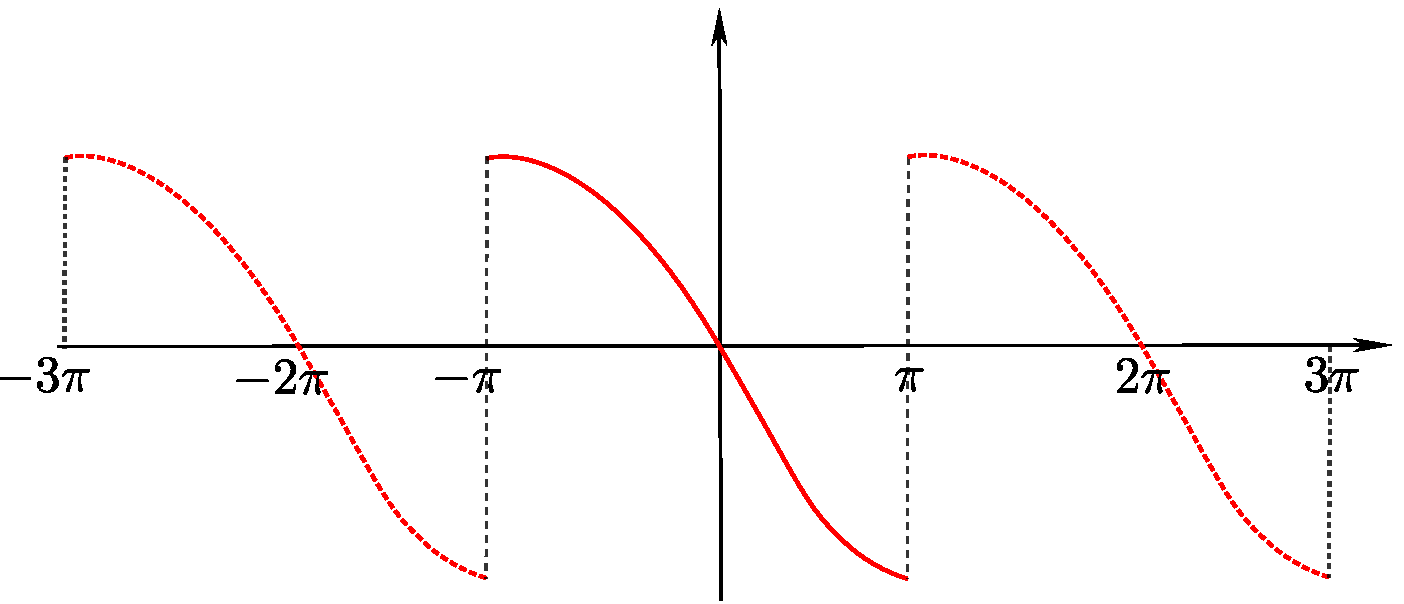
\includegraphics[scale = 0.45]{Figuras/Periocidad.pdf}
    \caption{Extensión periódica de una función real seccionalmente continua en $[-\pi,\pi]$.}
\end{figure}
\end{ejemplo}

% \subsection{Funciones pares e impares}
 
\begin{defi} \marginnote{Funciones pares e impares}
Sea $f: [-a,a] \longrightarrow \mathbb{R}$ perteneciente a $\mathscr{C}[-a,a]$.
Diremos que $f$ es una \textbf{función par} si y solo si, para todo $x$ en el intervalo $[-a,a]$, se cumple que
\begin{equation}
    f(-t) = f(t) \ .
\end{equation}
De forma similar, diremos que $f$ es una \textbf{función impar} si y solo si, para todo $x$ en el intervalo $[-a,a]$, se cumple que
\vspace{-0.1cm}
\begin{equation}
     f(-t) = -f(t) \ .
\end{equation}
\end{defi} 

\begin{propo}
    Sea $f: [-a,a] \longrightarrow \mathbb{R}$ integrable,
    \begin{align*}
        f ~\mbox{es par} &\Rightarrow \int_{-a}^a f(t) \,dt = 2 \int_0^a f(t) \,dt. \\
        f ~\mbox{es impar} &\Rightarrow \int_{-a}^a f(t) \,dt = 0.
    \end{align*}
\end{propo}

\begin{obs}{Observación}
    Toda función $f:[-a,a] \longrightarrow \mathbb{R}$ puede expresarse como la suma de una función par más otra impar: $f = f_p + f_i$ con 
    \begin{equation*}
        f_p(t) = \frac{f(t) + f(-t)}{2}, \quad f_i(t) = \frac{f(t) - f(-t)}{2} \ .
    \end{equation*}
\end{obs}

\begin{defi} \marginnote{Extensión par e impar}
Sea $f \in \mathscr{C}[0,a]$ real, entonces la \textbf{extensión par} y la \textbf{extensión impar} de $f$ están definidas, respectivamente, por:
\begin{equation*}
    E_f(t) = \left\{ \begin{array}{cll}
    f(-t)     & \mbox{si} & -a \leq t < 0 \\
    f(t)     & \mbox{si} & 0 \leq t \leq a
    \end{array} \right. , ~ O_f(t) = \left\{ \begin{array}{cll}
    -f(-t)     & \mbox{si} & -a \leq t < 0 \\
    f(t)     & \mbox{si} & 0 \leq t \leq a
    \end{array} \right. .
\end{equation*}
Ambas extensiones se encuentran definidas en el intervalo $[-a,a]$.
\end{defi}

\begin{figure}[H]
    \centering
    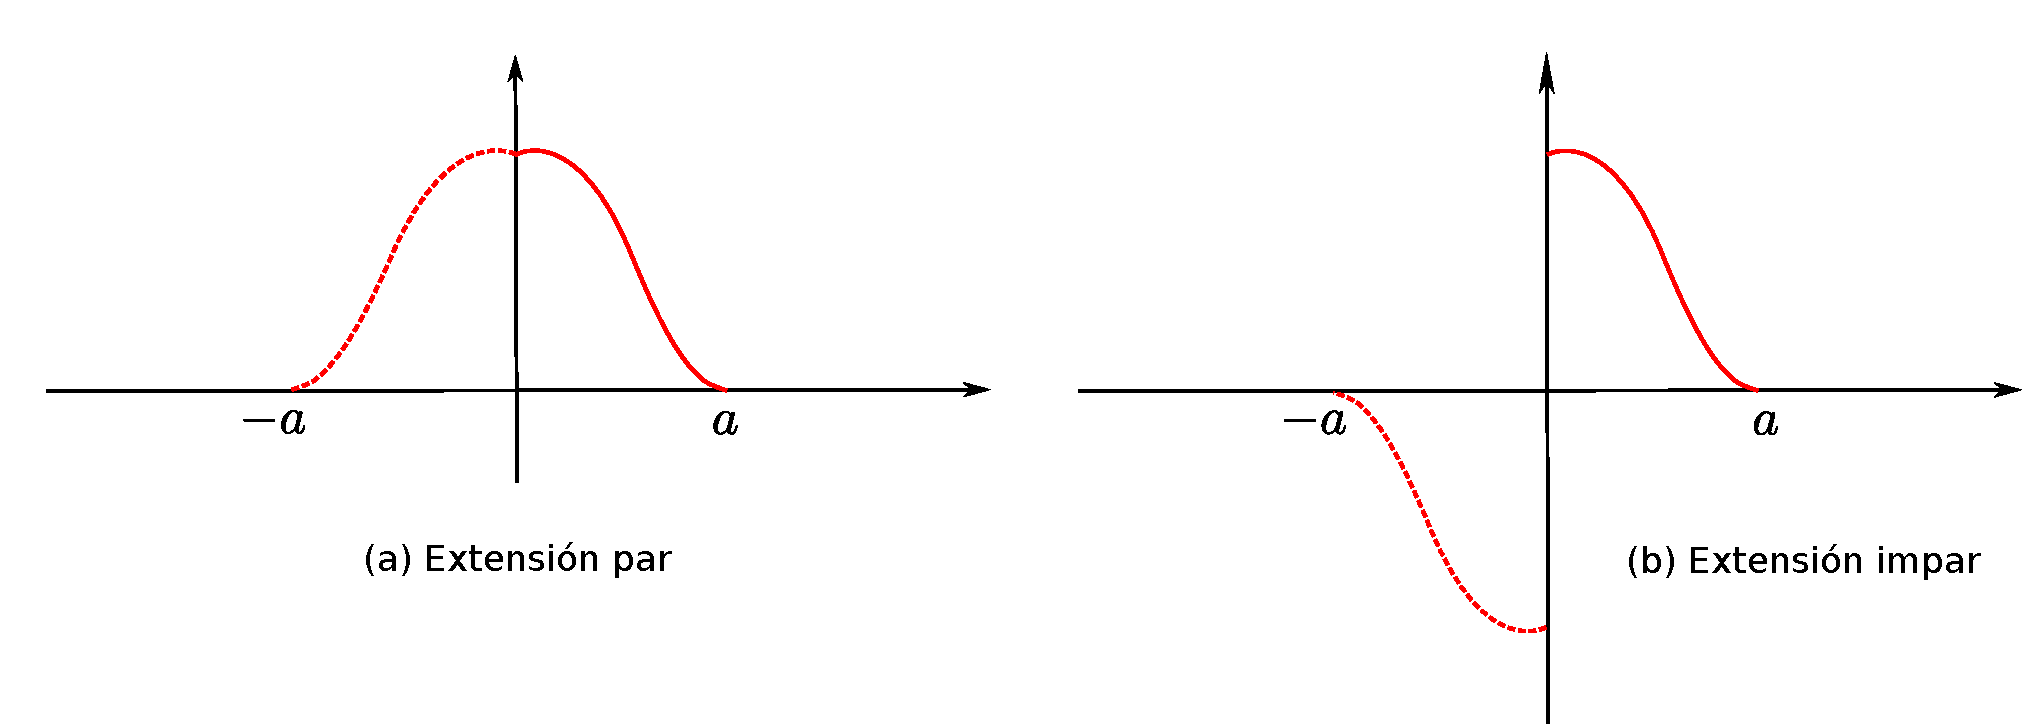
\includegraphics[width = \textwidth]{Figuras/Paridad.pdf}
    \caption{Extensión par e impar de una función real seccionalmente continua en $[0,a]$. }
\end{figure}

\subsection{Serie de Fourier trigonométrica}

% \subsection{Definición}

\begin{propo}
    En el espacio $\mathscr{C}[a,b]$, el conjunto formado por las funciones
    $$\left\{ 1, \cos\left( \frac{2n \pi}{T}x \right), \sin\left( \frac{2n \pi}{T}x \right) \right\}_{n=1}^{\infty}$$
    es un conjunto ortogonal, con $T = b-a$ el periodo de la función.
\end{propo}


\begin{defi} \marginnote{Sistema trigonométrico}
    Llamamos \textbf{sistema trigonométrico} al conjunto de funciones ortonormales en el espacio $\mathscr{C}[-\pi,\pi]$, definido como
    $$\left\{ \frac{1}{\sqrt{2\pi}}, \frac{\cos(nt)}{\sqrt{\pi}}, \frac{\sin(nt)}{\sqrt{\pi}} \right\}_{n=1}^{\infty}$$
\end{defi}

\begin{defi} \marginnote{Condiciones de Dirichlet}
    Una función $f$ satisface las llamadas \textbf{Condiciones de Dirichlet} si satisface
    \begin{enumerate}
        \item Se encuentra definida en un intervalo $(a,a+T)$.
        \item Tanto $f$ como su derivada son funciones seccionalmente continuas en el intervalo $(a,a+T)$.
        \item $f$ tiene un número finito de discontinuidades \emph{finitas}.
        \item $f$ es una función periódica de periodo $T$.
    \end{enumerate}

\end{defi}

\begin{defi} \marginnote{Serie de Fourier}
Sea $f \in \mathscr{C}[a, a+T]$ una función que satisface las condiciones de Dirichlet. Entonces, ella puede ser aproximada por la serie 
\begin{equation}
    \frac{a_0}{2} + \sum_{n=1}^{\infty} \left( a_n \cos\left( \frac{2n\pi}{T}x \right) + b_n \sin\left( \frac{2n\pi}{T}x \right) \right) \approx f(x) \ . \label{FourierTrigo}
\end{equation}

Esta expansión se denomina \textbf{serie trigonométrica de Fourier} o simplemente \textbf{serie de Fourier}, donde los \textit{coeficientes de Fourier} están dados por:
\begin{align*}
    a_0 &= \frac{2}{T} \int_{a}^{a+T} f(t) \,dt, \\
    a_n &= \frac{2}{T} \int_{a}^{a+T} f(t) \cos\left( \frac{2n\pi}{T}t \right) \,dt, \quad n = 1,2, \dots\\
    b_n &= \frac{2}{T} \int_{a}^{a+T} f(t) \sin\left( \frac{2n\pi}{T}t \right) \,dt. \quad n = 1,2, \dots
\end{align*}
\end{defi}

\begin{ejemplo} \label{EjemploFourier1}
    Consideremos la función $f(x) = x^2$ definida para $x\in [-\pi,\pi]$, la cual es continua con derivada $f'(x) = 2x$ también continua, luego la serie de Fourier de $f$ converge puntualmente a $f$ para todo $x \in (-\pi,\pi)$. Para los extremos $x = \pm \pi$ vemos que $f(\pi) = f(-\pi)$, por lo tanto la serie converge puntualmente a $f$ para todo $x \in [-\pi,\pi]$.
    
    Sus coeficientes de Fourier están dados por:
    \begin{align*}
        a_0 &= \frac{1}{\pi} \int_{-\pi}^{\pi} x^2 \,dx = \left. \frac{x^3}{3\pi} \right|_{-\pi}^{\pi} = \frac{2}{3} \pi^2, \\
        a_n &= \frac{1}{\pi} \int_{-\pi}^{\pi} x^2 \cos(n x)\,dx =   \left. \frac{1}{n\pi} x^2 \sin(nx)  \right|_{-\pi}^{\pi} - \frac{2}{n\pi} \int_{-\pi}^{\pi} x \sin(nx) \,dx\\
        &= \left.   \frac{2}{n^2\pi} x \cos(nx)\right|_{-\pi}^{\pi} - \frac{2}{n^2 \pi} \cancelto{0}{\int_{-\pi}^{\pi} \cos(nx) \,dx }\\
        &=  \frac{4}{n^2} \cos(n\pi) =  (-1)^n \frac{4}{n^2}, \quad n = 1,2,\dots\\
         b_n &= \frac{1}{\pi} \int_{-\pi}^{\pi} x^2 \sin(nx)\,dx = 0, \quad n = 1,2, \dots
    \end{align*}
    
    Entonces, su serie de Fourier es
    \begin{equation}
    f(x) = \frac{\pi^2}{3} + \sum_{n=1}^{\infty} (-1)^n \frac{4}{n^2} \cos(nx), \qquad x \in [-\pi,\pi].    \label{FourierCuadratica}
    \end{equation}
    
    Es claro que la serie de Fourier de $f(x) = x^2$ para todo $x\in \mathbb{R}$ representa la extensión periódica de los valores de $f(x)$ en el intervalo $[-\pi,\pi]$.
    
    La gráfica de $f$ en conjunto con diferentes sumas parciales de su serie de Fourier están representadas en la figura \ref{fig:EjemploFourier1}. 
    
    % \begin{figure}[htb]
        \centering
        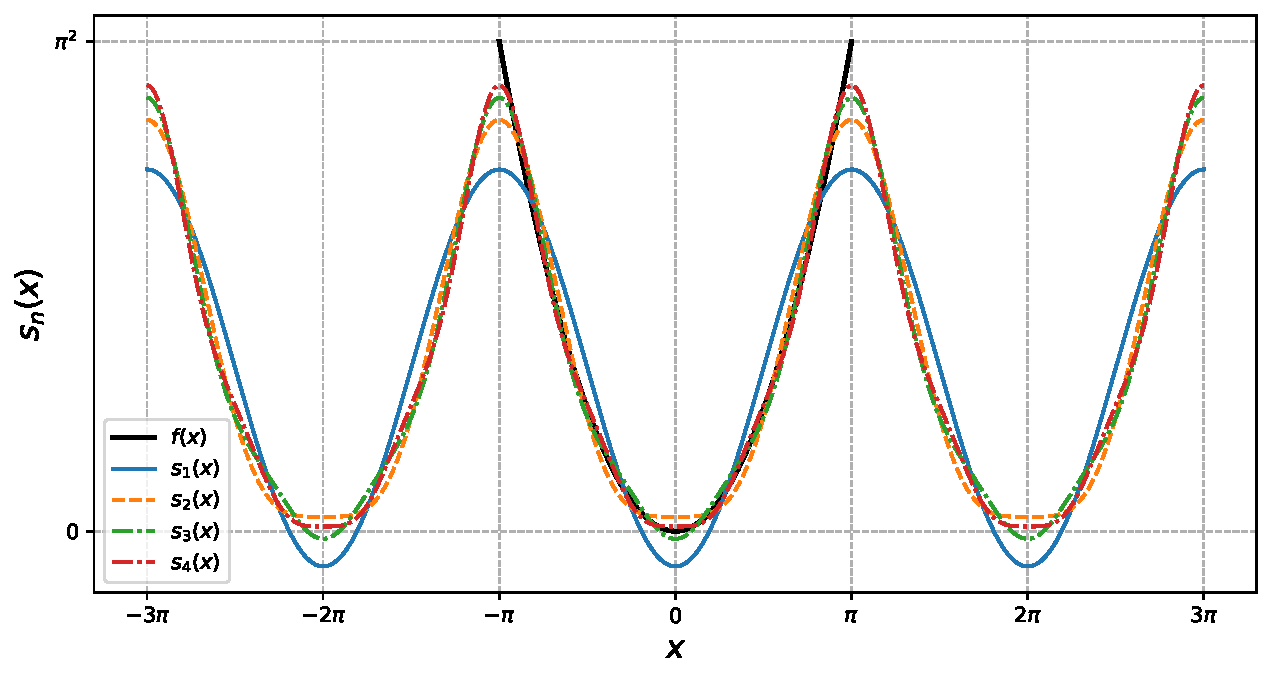
\includegraphics[width = 0.8\textwidth]{Figuras/EjemploFourier1.pdf}
        \captionof{figure}{Serie de Fourier de la función $f(x) = x^2, -\pi \leq x \leq \pi$, truncada hasta $n = 4$.}
        \label{fig:EjemploFourier1}
    % \end{figure}
    % El teorema visto para convergencia uniforme nos garantiza que esta serie converge uniformemente a $f(x) = x^2$ en $[-\pi,\pi]$, es más, al aplicar el criterio de M de Weierstrass a la serie, ésta converge para todo $x \in \mathbb{R}$, pues
    % $$\forall  x \in \mathbb{R}: ~ \left|(-1)^n \frac{4}{n^2} \cos(nx)\right| \leq \frac{4}{n^2} = M_n ~~\mbox{y}~~  \sum\limits_{n=1}^{\infty} M_n < \infty.$$
\end{ejemplo}

% \textbf{Observación}: La serie de Fourier de $f$ converge en media a $f$, o sea, 
% \begin{shaded}
% $$f(t) \sim \frac{a_0}{2} + \sum_{n=1}^{\infty} (a_n \cos(nt) + b_n \sin(nt)).$$    
% \end{shaded}

% \begin{propo} \label{C.FourierCero}
% Los coeficientes de la serie trigonométrica de Fourier de $f \in \mathscr{C}[-\pi,\pi]$ convergen a cero cuando $n \to \infty$, es decir,
% $$\lim_{n \to + \infty} a_n = \lim_{n \to + \infty} b_n = 0.$$
% \end{propo}

% \begin{demo}
% Si denotamos el sistema trigonométrico por 
% $$\varphi_0(t) = \frac{1}{\sqrt{2\pi}}, ~ \varphi_{2n-1}(t) = \frac{1}{\sqrt{\pi}} \cos(nt), ~ \varphi_{2n(t)} = \frac{1}{\sqrt{\pi}} \sin(nt), \quad n = 1,2, \dots$$

% tenemos que la serie generalizada de Fourier queda
% $$\sum_{n=0}^{\infty} C_n \varphi_n(t) = C_0 \varphi_0(t) + \sum_{n=1}^{\infty} \left[ C_{2n-1} \varphi_{2n-1}(t) + C_{2n} \varphi_{2n}(t) \right] ,$$

% la cual corresponde a la serie trigonométrica de Fourier de $f \in \mathscr{C}[-\pi,\pi]$, donde 
% $$a_0 = \sqrt{\frac{2}{\pi}} C_0, ~ a_n = \frac{C_{2n-1}}{\sqrt{\pi}}, ~ b_n = \frac{C_{2n}}{\sqrt{\pi}}, \quad n = 1,2, \dots$$

% De lo discutido en el primer capítulo, una de las consecuencias de la desigualdad de Bessel \eqref{D.Bessel} es que 
% $$\lim_{n \to + \infty} C_n = \lim_{n \to + \infty} \langle f, \varphi_n \rangle = 0 ~\Rightarrow~ \lim_{n \to \infty} C_{2n-1} = \lim_{n \to \infty} C_{2n} = 0. $$

% Por lo tanto, 
% $$\lim_{n \to + \infty} a_n = \lim_{n \to + \infty} b_n = 0.$$

% \end{demo}

% ¿Convergerá puntual y/o uniformemente la serie de Fourier a $f(t)$? ¿Qué condiciones deben cumplirse?

% Antes de responder estas preguntas, primero justifiquemos que es suficiente trabajar con funciones a valores reales, a pesar de que los siguientes teoremas también son válidos para funciones a valores complejos. 

\subsubsection{Serie de Fourier de una función compleja de variable real}

Sea $f = u + iv \in \mathscr{C}[a,b]$, su serie de Fourier trigonométrica está dada por \eqref{FourierTrigo} con 
\begin{align*}
    a_0 &= \frac{2}{T} \int_{a}^{b} f(t) \,dt =  \frac{2}{T} \int_a^b u(t) \,dt + i\frac{2}{T} \int_a^b v(t) \,dt,\\
    a_n &= \frac{2}{T} \int_a^b f(t) \cos\left( \frac{2n\pi}{T}t \right) \,dt = \frac{2}{T} \int_a^b u(t) \cos\left( \frac{2n\pi}{T}t \right) \,dt + i\frac{2}{T} \int_a^b v(t) \cos\left( \frac{2n\pi}{T}t \right) \,dt , \quad n \in \mathbb{N} \\
    b_n &= \frac{2}{T} \int_a^b f(t) \sin\left( \frac{2n\pi}{T}t \right) \,dt = \frac{2}{T} \int_a^b u(t) \sin\left( \frac{2n\pi}{T}t \right) \,dt + i\frac{2}{T} \int_a^b v(t) \sin\left( \frac{2n\pi}{T}t \right) \,dt, \quad n \in \mathbb{N}
\end{align*}

Entonces, su serie de Fourier nos queda
\begin{align}
  f(t) & \sim   \left\{ \frac{\real(a_0)}{2} + \sum_{n=1}^{\infty} \left[ \real(a_n) \cos\left( \frac{2n\pi}{T}t \right) + \real\left( b_n \right) \sin\left( \frac{2n\pi}{T}t \right) \right] \right\}  \nonumber \\
   & \qquad + i \left\{ \frac{\im(a_0)}{2} + \sum_{n=1}^{\infty} \left[\im(a_n) \cos\left( \frac{2n\pi}{T}t \right) + \im(b_n) \sin\left( \frac{2n\pi}{T}t \right) \right] \right\},
\end{align}

es decir, la serie de Fourier de $f = u + iv$ será dada por
\begin{equation}
    S_F(f) = S_F(u) + i S_F(v) \ ,
\end{equation}
donde $S_F$ representa a una serie de Fourier.


\subsection{Series de senos y cosenos}

\begin{defi} \marginnote{Serie de Fourier seno y serie de Fourier coseno}
    Dadas las extensiones par e impar de una función, $E_f, O_f: [a,b] \to \mathbb{R}$, es posible obtener el desarrollo en serie de Fourier de cada una de estas, que corresponden a los \textbf{desarrollos en serie de Fourier de coseno y de seno} de $f$, respectivamente. Estos son definidos como
    \begin{align*}
        E_f(t) & \sim \frac{a_0}{2}  + \sum_{n=1}^{\infty} a_n \cos\left( \frac{2n\pi}{T}t \right), & ~~\mbox{donde}~~ a_n = \frac{2}{T} \int_a^{b} f(t) \cos\left( \frac{2n\pi}{T}t \right)  dt \ , \\
        O_f(t) & \sim  \sum_{n=1}^{\infty} b_n \sin\left( \frac{2n\pi}{T}t \right), & ~~\mbox{donde} ~~ b_n = \frac{2}{T} \int_a^{b} f(t) \sin\left( \frac{2n\pi}{T}t \right) \ dt \ .
    \end{align*}

    En ambos casos, se ha hecho uso de las propiedades de las funciones pares e impares para hallar los coeficientes de las series.
\end{defi}

% Puesto que $E_f, O_f: [-\pi,\pi] \to \mathbb{R}$ son seccionalmente continuas, se puede obtener el desarrollo en serie de Fourier de estas, los cuales están definidos por: \footnote{La forma de las series seno y coseno, con sus respectivos coeficientes, se obtienen al aplicar las propiedades vistas para las funciones pares e impares.}
% $$ 

% y
% $$ .$$

% Estos son llamados \textbf{desarrollos en serie de Fourier de coseno y de seno de $f$}, respectivamente.

% \subsection{Convergencia puntual y uniforme}

% \begin{defi}
% Sea $f: [a,b] \longrightarrow \mathbb{R}$, para $t_0 \in [a,b]$ definimos
% \begin{align*}
%     f(t_0^+) &= \lim_{t \to t_0^+} f(t), \\
%     f(t_0^-) &= \lim_{t \to t_0^-} f(t),
% \end{align*}

% si existen los límites. 

% Una discontinuidad en $t_0$ tal que $f(t_0^+)$ y $f(t_0^-)$ existen se denomina \textbf{discontinuidad de salto} y $f(t_0^+) - f(t_0^-)$ recibe el nombre de \textbf{salto} de $f$ en $t_0$.
% \end{defi}

% \textbf{Observaciones:} 

% \begin{enumerate}
%     \item La magnitud del salto es $|f(t_0^+) - f(t_0^-)|$.
    
%     \item El salto se anula cuando $f(t_0) = f(t_0^+) = f(t_0^-)$, es decir, cuando $f$ es continua en $t_0$.
    
%     \item Una función $f: [a,b] \longrightarrow \mathbb{R}$ seccionalmente continua tiene discontinuidades de salto.
% \end{enumerate}

% \begin{defi}
% Sea $f:[a,b] \longrightarrow \mathbb{R}$, con una discontinuidad de salto en $t_0 \in [a,b]$, definimos la \textbf{derivada por la derecha} como 
% $$f'(t_0^+) = \lim_{h \to 0^+} \frac{f(t_0 + h ) - f(t_0^+)}{h}$$

% cuando el límite existe. Similarmente, definimos la \textbf{derivada por la izquierda} como 
% $$f'(t_0^-) = \lim_{h \to 0^-} \frac{f(t_0 + h ) - f(t_0^-)}{h}$$

% cuando el límite existe.
% \end{defi}

% \begin{teorema}[Convergencia puntual de la serie de Fourier] \label{Puntual}
% Sea $f(t)$ una función real seccionalmente continua en el intervalo $-\pi < t < \pi$. Su serie de Fourier trigonométrica converge al valor medio
% \vspace{-0.05cm}
% $$\frac{f(t^+) + f(t^-)}{2}$$

% para cada $t \in (-\pi,\pi)$ donde ambas derivadas laterales $f'(t^+)$ y $f'(t^-)$ existen.
% \end{teorema}

% \textbf{Observación:} Si denotamos por $f_e$ a la extensión periódica de $f$, a partir del teorema anterior, la expansión en serie de Fourier converge a $f_e$ para todo $x \in \mathbb{R}$ al extenderla periódicamente al valor medio
% $$\frac{f_e(t^+) + f_e(t^-)}{2}.$$

% De hecho, en los extremos $t = \pm \pi$, la serie converge a 
% $$\frac{f(-\pi^+) + f(\pi^-)}{2}.$$

% En efecto, observemos que
% $$f_e(-\pi^+) = f(-\pi^+) ~~\mbox{y}~~ f_e(-\pi^-) = f(\pi^-).$$

% Luego, el cociente
% $$\frac{f_e(-\pi^+) + f_e(-\pi^-)}{2} = \frac{f(-\pi^+) + f(\pi-)}{2}.$$

% Análogamente para $t = \pi$.

% \begin{teorema}[Convergencia uniforme] \label{C.Uniforme}
% Supóngase que $f$ es continua en $[-\pi,\pi]$, $f(-\pi) = f(\pi)$ y que $f'$ es continua por tramos, con discontinuidades de salto. Entonces la serie de Fourier trigonométrica de $f$ converge a $f$ absolutamente y uniformemente.
% \end{teorema}

% \subsection{Ejemplos}



% Podemos usar la expansión en serie de Fourier de $f(x) = x^2$ en $[-\pi,\pi]$ para probar que 
% $$\sum_{n=1}^{\infty} \frac{1}{n^2} = 1 + \frac{1}{4} + \frac{1}{9} + \cdots = \frac{\pi^2}{6}.$$

% En efecto, al evaluar $x = \pi$ en \eqref{FourierCuadratica}, obtenemos que 
% $$f(\pi) = \frac{\pi^2}{3} + \sum_{n=1}^{\infty} (-1)^n \frac{4}{n^2} \cos(n\pi) = \frac{\pi^2}{3} + \sum_{n=1}^{\infty} (-1)^{2n} \frac{4}{n^2} = \frac{\pi^2}{3} +  \sum_{n=1}^{\infty} \frac{4}{n^2}.$$

% Así,
% $$\pi^2 = \frac{\pi^2}{3} + 4 \sum_{n=1}^{\infty} \frac{1}{n^2} \Rightarrow \sum_{n=1}^{\infty} \frac{1}{n^2} = \frac{\pi^2}{6}.$$

\begin{ejemplo} \label{Signo}
Consideremos la función signo  definida por
$$f(x) := \left\{ \begin{array}{cc}
     -1,& - \pi \leq x < 0  \\
     1,&   0 \leq x \leq \pi
\end{array} \right. .$$

La función es seccionalmente continua con $x = 0$ punto de discontinuidad de salto y las derivadas laterales existen para todo $x \in (-\pi,\pi)$, luego la serie de Fourier de $f$ converge puntualmente a $f$ en los puntos de continuidad y a 
$$\frac{f(0^-) + f(0^+)}{2} = 0, \quad \mbox{en} ~ x = 0 ~~\mbox{y}$$
$$\frac{f(-\pi^+) + f(\pi^-)}{2} = 0, \quad \mbox{en} ~ x = \pm \pi. $$

Sus coeficientes de Fourier están dados por:
\begin{align*}
    a_0 &= \frac{1}{\pi} \int_{-\pi}^{\pi} f(x) \,dx = 0 , \\
    a_n &= \frac{1}{\pi} \int_{-\pi}^{\pi} f(x) \cos(n x)\,dx = 0, \quad n = 1,2,\dots
\end{align*}
\begin{align*}
     b_n &= \frac{1}{\pi} \int_{-\pi}^{\pi} f(x) \sin(nx) \,dx \\
     &= \frac{1}{\pi} \int_{-\pi}^0 (-1) \sin(nx)\,dx + \frac{1}{\pi} \int_{0}^{\pi} (1) \sin(nx) \,dx \\
     &= \left.  \frac{1}{\pi n} \cos(nx) \right|_{-\pi}^0 - \left. \frac{1}{\pi n} \cos(nx) \right|_{0}^{\pi} \\
     &= \frac{2}{\pi n} [1 - (-1)^n] \\
     &= \left\{ \begin{array}{cl}
         0, & n ~\mbox{par}  \\
         \frac{4}{\pi n}, &  n ~\mbox{impar}
     \end{array} \right. .
\end{align*}

Entonces, su serie de Fourier es 
$$f(x) =  \sum_{n ~impar} \frac{4}{\pi n} \sin(nx) = \sum_{k=1}^{\infty} \frac{4}{\pi} \frac{\sin[(2k-1)x]}{ (2k-1)}.$$

\textbf{Aclaración:} Note que a pesar de haber escrito que la función $f$ es igual a la serie, debemos tener en cuenta que en los punto $x = 0$ y $x = \pm \pi$ converge al valor medio del salto de la discontinuidad.

Es claro que la serie de Fourier de $f$ para todo $x\in \mathbb{R}$ representa la extensión periódica de los valores de $f(x)$ en el intervalo $[-\pi,\pi]$.

La gráfica de $f$ en conjunto con diferentes sumas parciales de su serie de Fourier están representadas en la figura \ref{fig:EjemploFourier2}.

\begin{figure}[H]
    \centering
    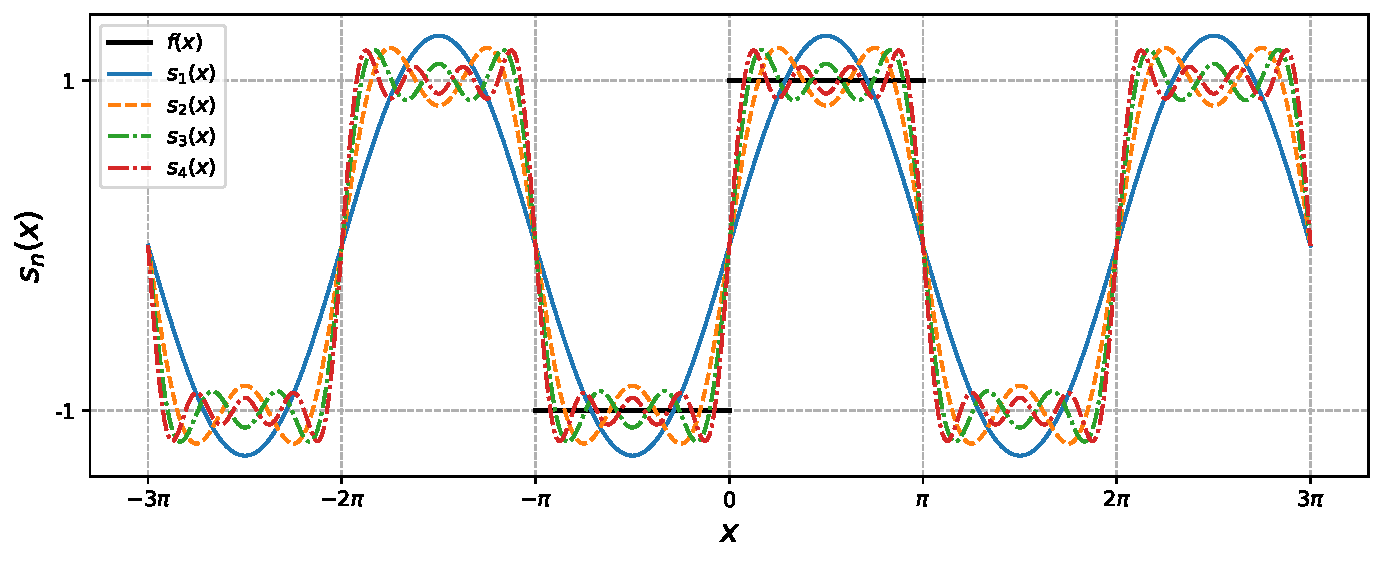
\includegraphics[scale = 0.65]{Figuras/EjemploFourier2.pdf}
    \caption{Serie de Fourier de la función signo truncada hasta $n = 4$.}
     \label{fig:EjemploFourier2}
\end{figure}

\end{ejemplo}

\subsection{Serie exponencial}

\begin{propo}
    En el espacio $\mathscr{C}[a,a+T]$, el conjunto formado por las funciones 
    \begin{equation}
        \left\{ \frac{1}{\sqrt{T}} \exp\left(i\frac{2n\pi}{T}x\right) \right\}_{n= - \infty}^{n = \infty}
    \end{equation}
    es un conjunto ortonormal.
\end{propo}

\begin{defi} \marginnote{Sistema exponencial}
    Llamamos \textbf{sistema exponencial} al conjunto de funciones ortonormales en el espacio $\mathscr{C}[-\pi,\pi]$, definido como 
    $$\left\{ \frac{1}{\sqrt{2\pi}} e^{int} \right\}_{n= - \infty}^{n = \infty}$$
\end{defi}

\begin{defi} \marginnote{Serie de Fourier exponencial}
Sea $f \in \mathscr{C}[a,a+T]$ una función con un número finito de discontinuidades. Entonces, ella puede ser aproximada por la serie 
\begin{equation}
     \sum_{n=- \infty}^{\infty} c_n \exp\left(i\frac{2n\pi}{T}x\right) \label{FourierExpo}
\end{equation}

Esta expansión se denomina \textbf{serie exponencial de Fourier}  donde los \textit{coeficientes de Fourier} están dados por:
\begin{equation*}
    c_n = \frac{1}{T} \int_{a}^{a+T} f(t) \exp\left(-i\frac{2n\pi}{T}t \right) \ dt \ .
\end{equation*}
\end{defi}

% \textbf{Observación}: La serie de Fourier de $f$ converge en media a $f$, o sea, 
% \begin{shaded}
%  $$f(t) \sim \sum_{n=- \infty}^{\infty} c_n e^{int}.$$   
% \end{shaded}

\begin{propo} \label{TrigoExpo}
La $n$-ésima suma parcial de la serie de Fourier trigonométrica de una función (real o compleja) es igual a la $n$-ésima suma parcial de la serie exponencial.
\end{propo}

\begin{demo}
La $n$-ésima suma parcial de la serie exponencial es
$$ s_n(t) = \sum_{k=-n}^n c_k e^{ikt}.$$

Separando la suma:
\begin{align*}
    s_n(t) &= \sum_{k=-n}^{-1} c_k e^{ikt} + c_0 + \sum_{k=1}^n c_k e^{ikt} \\
    &= c_0 + \sum_{k=1}^n c_k e^{ikt} + \sum_{k=1}^n c_{-k} e^{-ikt} \\
    &= c_0 + \sum_{k=1}^n [c_k e^{ikt} + c_{-k} e^{-ikt}]. 
\end{align*}

Usando la identidad de Euler, $e^{i\theta} = \cos(\theta) + i \sin(\theta)$, encontramos que
$$s_n(t) = c_0 +  \sum_{k=1}^n [(c_k + c_{-k}) \cos(kt) + i(c_k - c_{-k}) \sin(kt)].$$

Desarrollando los coeficientes de la serie exponencial de Fourier, tenemos que
\begingroup
\allowdisplaybreaks
\begin{align*}
    c_0 &= \frac{1}{2\pi} \int_{-\pi}^{\pi} f(t) \,dt, \\
    c_k + c_{-k} &= \frac{1}{2\pi} \int_{-\pi}^{\pi} f(t) e^{-ikt} \,dt + \frac{1}{2\pi} \int_{-\pi}^{\pi} f(t) e^{ikt} \,dt  \\
    &= \frac{1}{2\pi} \int_{-\pi}^{\pi} f(t) [e^{ikt} + e^{-ikt}] \,dt \\
    &= \frac{1}{\pi} \int_{-\pi}^{\pi} f(t) \cos(kt) \,dt; \quad k = 1,2, \dots\\
   i( c_k - c_{-k}) &= \frac{i}{2\pi} \int_{-\pi}^{\pi} f(t) e^{-ikt} \,dt - \frac{i}{2\pi} \int_{-\pi}^{\pi} f(t) e^{ikt} \,dt \\
   &= - \frac{i}{2\pi} \int_{-\pi}^{\pi} f(t) [e^{ikt} - e^{-ikt}] \,dt \\
   &= \frac{1}{\pi} \int_{-\pi}^{\pi} f(t) \sin(kt)\,dt; \quad k = 1,2, \dots
\end{align*}
\endgroup

Comparando las expresiones obtenidas con los coeficientes de la serie de Fourier trigonométrica, podemos concluir que 
$$c_0 = \frac{a_0}{2}, ~  c_k + c_{-k} = a_k, ~ i( c_k - c_{-k}) = b_k; \quad k = 1,2, \dots$$

Por lo tanto, 
$$ s_n(t) = \sum_{k=-n}^n c_k e^{ikt} = \frac{a_0}{2} + \sum_{k=1}^n (a_k \cos(kt) + b_k \sin(kt)).$$

\end{demo}
Una consecuencia inmediata de la proposición \ref{TrigoExpo} es que todos los teoremas vistos para la serie de Fourier trigonométrica son aplicables a la serie de Fourier exponencial.

\begin{propiedad} 
    \textbf{Propiedades de la Serie de Fourier exponencial}
    \begin{enumerate}
        \item Los coeficientes de las series \eqref{FourierTrigo} y \eqref{FourierExpo} están relacionados por 
        \begin{equation}
        a_0 = 2c_0,~~ a_n = c_n + c_{-n}, ~~ b_n = i(c_n - c_{-n}); \quad n = 1,2, \dots    \label{RelacionCoefi1}
        \end{equation}
        
        o bien, 
        \begin{equation}
            c_n = \left\{ \begin{array}{cl}
                \frac{1}{2} (a_n - ib_n), & n \geq 0  \\
            \frac{1}{2}(a_{-n} + i b_{-n}),     & n  \leq -1 
            \end{array} \right. . \label{RelacionCoefi2}
        \end{equation}

        \item Si $f(t)$ es una función real, entonces sus respectivos coeficientes complejos $c_n$ satisfacen la relación:
        $$c_n^* = \frac{1}{2\pi} \int_{-\pi}^{\pi} f(t) (e^{-int})^* \,dt = \frac{1}{2\pi} \int_{-\pi}^{\pi} f(t) e^{int} \,dt = c_{-n}\ .$$
    \end{enumerate}
\end{propiedad}




\section{Transformada de Fourier}

En el capítulo anterior, aprendimos que la serie de Fourier de $f \in \mathscr{C}[-L/2,L/2]$ está dada por 
\begin{equation} \label{Transformada1}
  f(x) = \sum_{n=-\infty}^{\infty} c_n e^{i \frac{2n\pi}{L}x} \ ,  
\end{equation}
donde 
\begin{equation} \label{Transformada2}
  c_n = \frac{1}{L} \int_{-L/2}^{L/2} f(x) e^{-i\frac{2n\pi}{L}x} \,dx, \quad n \in \mathbb{Z} \ . 
\end{equation}

Una consecuencia inmediata de la expansión en serie de Fourier es que la función $f(x)$ representada por la serie resulta periódica, con período $L$. Por lo tanto, decimos que la serie de Fourier permite \emph{expandir funciones periódicas}. 

Sin embargo, no todas las funciones son periódicas, y nos interesará expandirlas dentro de algún intervalo de validez. Necesitamos, entonces, algún modo de expandir, en una base ortonormal, funciones no periódicas. 

Podemos decir que el conjunto de coeficientes $\{c_n\}$ también definen a $f(x)$. Este conjunto de números $c_n$ puede ser entendido como una función en la variable $n$, escrita como $c(n)$, definida para un conjunto \emph{discreto} de valores de la variable independiente (en lugar de un intervalo continuo).  
\begin{defi}\marginnote{Espectro de Fourier}
    Se define como el \textbf{espectro de Fourier} a la función de variable discreta $c(n)$, definida a partir de los coeficientes de Fourier \eqref{Transformada2}.
\end{defi}

El espectro de una función puede ser graficado, asumiendo $c(n)$ real, como se observa en la figura \ref{fig:espectro-fourier}.

\vspace{-0.5cm}
\begin{figure}[H]
    \centering
    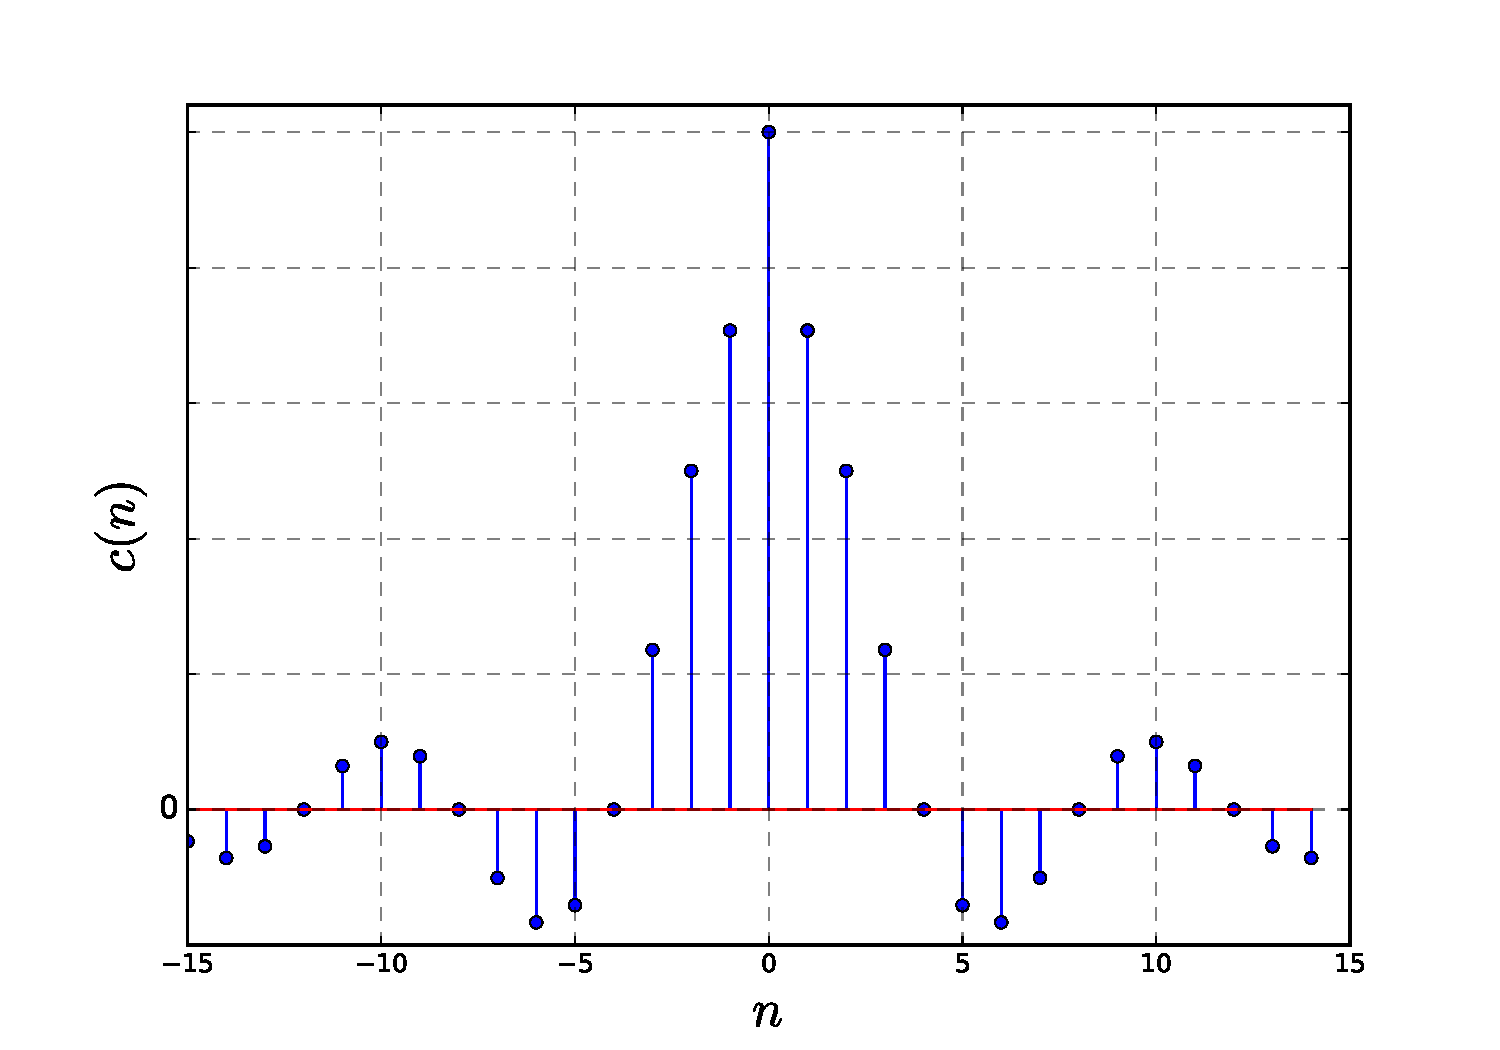
\includegraphics[width = 12cm]{Figuras/Espectro1.pdf}
    \caption{Espectro de Fourier.}
    \label{fig:espectro-fourier}
\end{figure}

En lugar de graficar $c$ vs $n$, podemos graficar $c$ vs $k$, el \emph{número de onda}, que corresponde a la frecuencia asociada a la parte espacial:
$$k = \frac{2\pi n}{L}.$$

Si $L \to \infty$, entonces las frecuencias se encuentran estrechamente espaciadas debido a que la diferencia entre valores consecutivos de $k$ es
$$\Delta k = \frac{ 2\pi \Delta n}{L}  = \frac{2\pi}{L}, \quad \mbox{pues}~ \Delta n = 1.$$

En otras palabras, para $L \to \infty$, $\Delta k$ es pequeño. Con este cambio de escala, el espectro de Fourier puede parecerse a lo mostrado en la figura \ref{Espectro1}.

\begin{figure}
    \centering
    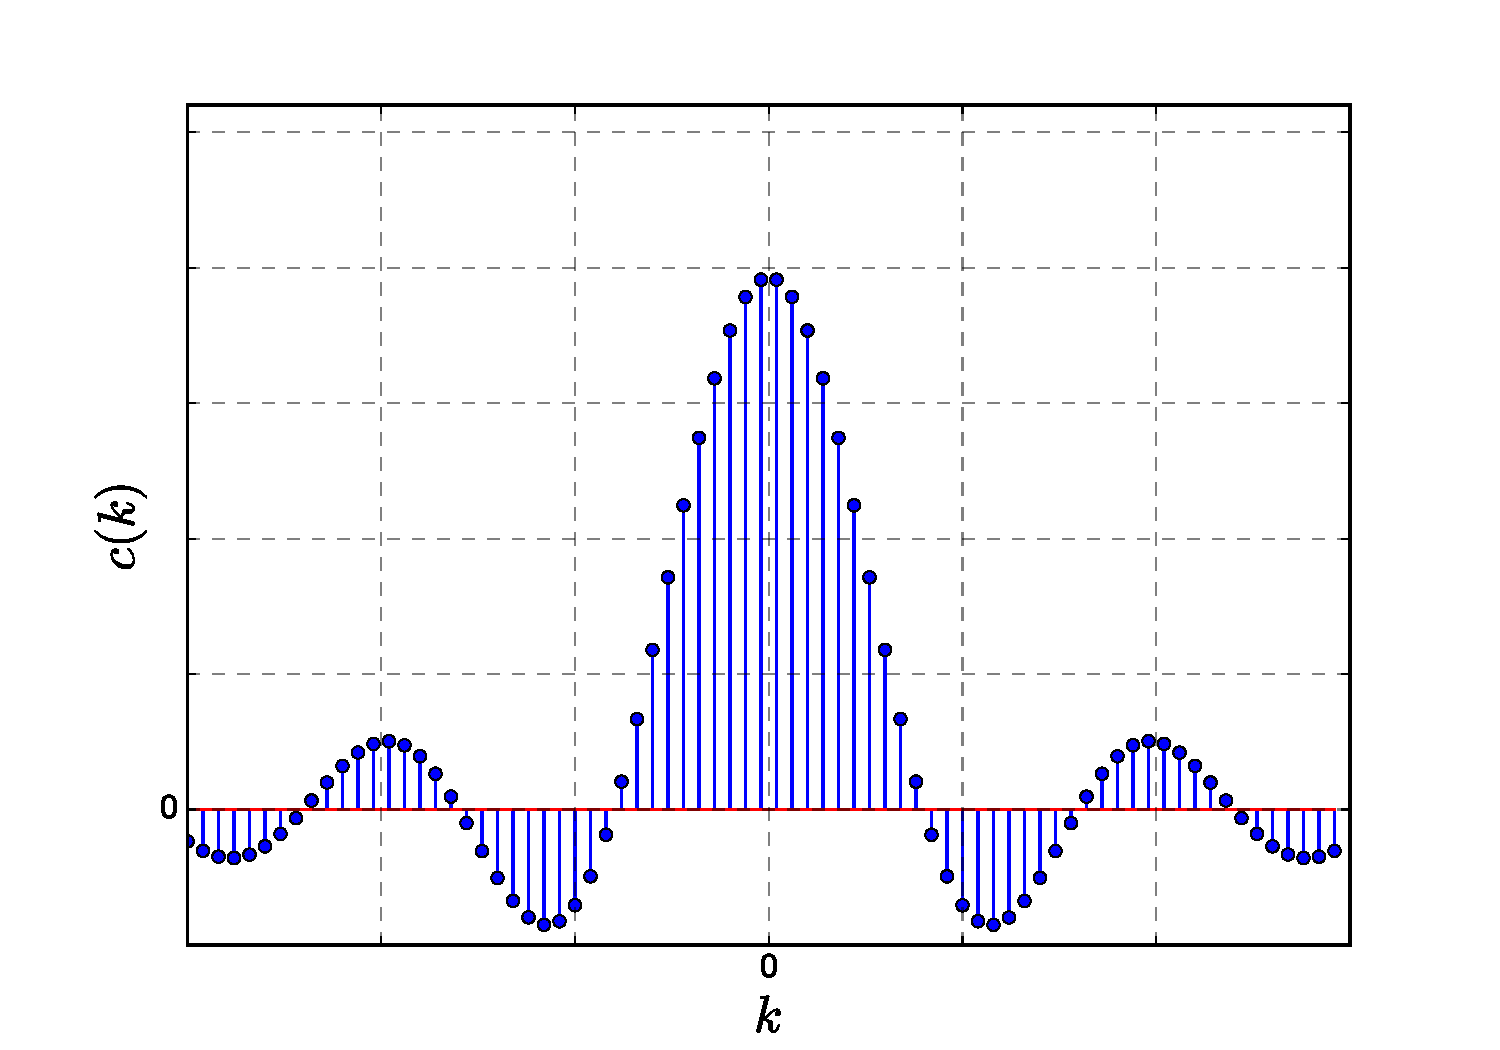
\includegraphics[scale = 0.4]{Figuras/Espectro2.pdf}
    \caption{Espectro de Fourier cuando $L \to + \infty$.}
    \label{Espectro1}
\end{figure}

Es natural especular sobre la posibilidad de un espectro continuo cuando $L$ tiende al infinito  de tal forma que todas las frecuencias están presentes. Puede ser instructivo considerar la siguiente derivación heurística: Sabemos que una función puede ser expandida como una serie de Fourier tal como se muestra en \eqref{Transformada1}. Luego, la transición $L \to \infty$ puede resultar difícil de realizar directamente ya que $c_n$ aparentemente tiende a cero. Seguimos entonces la idea de usar las frecuencias $k = 2\pi n/L$ tal que
$\Delta k = (2\pi/L ) \Delta n = 2\pi/L$ para valores de $k$ adyacentes y definimos
\begin{equation}
    c_L(k) = \frac{L}{\sqrt{2 \pi}} c_n \ .
\end{equation}

Usando las definiciones anteriores en las ecuaciones \eqref{Transformada1} y \eqref{Transformada2}, obtenemos que la función y sus coeficientes de Fourier se pueden escribir como: 
\begin{align*}
    f(x)&= \sum_{Lk/2\pi = -\infty}^{\infty} \frac{\sqrt{2\pi}}{L} c_L(k) e^{ikx} \left( \frac{\Delta k L}{2\pi}\right) = \sum_{Lk/2\pi = -\infty}^{\infty}  \frac{1}{\sqrt{2\pi}} c_L(k) e^{ikx} \Delta k , \\
  c_L(k) &= \frac{L}{\sqrt{2\pi}} \frac{1}{L} \int_{-L/2}^{L/2} f(x) e^{-ikx} dx = \frac{1}{\sqrt{2\pi}} \int_{-L/2}^{L/2} f(x) e^{-ikx} dx.
\end{align*}

Al hacer $L \to \infty$, la función $f$ puede considerarse como una función no-periódica arbitraria definida en todo el intervalo $(-\infty, \infty)$, mientras que la primera suma ``se convierte'' en una integral:
\begin{align*}
    f(x)& = \frac{1}{\sqrt{2\pi}} \int_{-\infty}^{\infty} c(k) e^{ikx} \,dk, \\
  c(k) & = \lim_{L\to + \infty} c_L(k) = \frac{1}{\sqrt{2\pi}} \int_{-\infty}^{\infty} f(x) e^{-ikx} dx.
\end{align*}

\begin{defi} \marginnote{Transformada de Fourier}
    Dada una función $f$ no periódica definida en $\mathscr{C}(-\infty, \infty)$, definimos su \textbf{transformada de Fourier} como 
    \begin{equation}\label{T.Fourier}
        \boxed{\tilde{f}(k) := \frac{1}{\sqrt{2\pi}} \int_{-\infty}^{\infty} f(x) e^{-ikx} dx \ .} 
    \end{equation}  
\end{defi}

Note que la transformada de Fourier es la extensión natural del concepto de series de Fourier para funciones no periódicas. Además, al ser $n$ una variable discreta, y $k$ continua, podemos decir que la transformada de Fourier es la generalización del concepto de series de Fourier cuando las funciones pertenecen a un espacio vectorial de dimensión continua.

\begin{defi}\marginnote{Transformada inversa de Fourier}
    Se define la \textbf{transformada inversa de Fourier} como
      \begin{equation}\label{I.Fourier}
     \boxed{f(x) = \frac{1}{\sqrt{2\pi}} \int_{-\infty}^{\infty} \tilde{f}(k) e^{ikx} \,dk \ .} 
    \end{equation}  
\end{defi}

\begin{obs}{Observaciones}
    \begin{itemize}
        \item Otras notaciones usadas son: $\tilde{f}(k) = \hat{f}(k) = g(k) = \mathcal{F}\{f(x)\}(k)$.
        
        \item El factor $1/\sqrt{2\pi}$ en la definición \eqref{T.Fourier} es convencional. Lo importante es que se cumpla la identidad conocida como \textbf{integral de Fourier}
        \begin{equation}
            f(x) = \int_{-\infty}^{\infty} \left[\frac{1}{2\pi} \int_{-\infty}^{\infty} f(\xi) e^{-ik\xi} d\xi \right] e^{ikx} \,dk.
          \label{IntegralFourier}
        \end{equation}
       
        % Por ejemplo, en lugar de estos factores, podría introducirse un $\alpha$ en \eqref{I.Fourier} y $1/(2\pi \alpha)$ en \eqref{T.Fourier}, con $\alpha$ una constante arbitraria. Algunas elecciones populares son: $\alpha = 1$ y $\alpha = 1/\sqrt{2\pi}$ \cite{Rubilar}.
    
        \item Al igual que el factor $1/\sqrt{2\pi}$ en la definición \eqref{T.Fourier}, la función $e^{-ikx}$ es convencional y puede ser reemplazada por $e^{ikx}$, siempre y cuando se verifique \eqref{IntegralFourier} \cite{Butkov, Riley}.
        
        % \item En el caso que $f(x)$ sea real, tenemos que \eqref{IntegralFourier} se puede escribir como 
        % \begin{equation}
        %     f(x) = \frac{1}{\pi} \int_{0}^{\infty} \int_{-\infty}^{\infty} f(\xi) \cos k(x-\xi)  \, d\xi \,dk.  \label{IntegralFourierReal}
        % \end{equation}
    
        % \colorlet{shadecolor}{blue!10} 
        % \begin{shaded}
        % En efecto, la relación \eqref{IntegralFourier} también se puede expresar como 
        % $$f(x) = \frac{1}{2\pi}  \int_{-\infty}^{\infty} \int_{-\infty}^{\infty} f(\xi) e^{-ik\xi} e^{ikx} d\xi  \,dk = \frac{1}{2\pi}  \int_{-\infty}^{\infty} \int_{-\infty}^{\infty} f(\xi) e^{ik(x-\xi)} d\xi  \,dk.$$
        
        % Como $f(x)$ es real, se igualan las partes reales para así obtener
        % $$f(x) = \frac{1}{2\pi} \int_{-\infty}^{\infty} \int_{-\infty}^{\infty} f(\xi) \cos k(x-\xi) d\xi  \,dk. $$
        
        % Puesto que $\cos k(x-\xi)$ es par con respecto a $k$, tenemos que 
        % $$f(x) = \frac{2}{2\pi} \int_{0}^{\infty} \int_{-\infty}^{\infty} f(\xi) \cos k(x-\xi)  \, d\xi \,dk =\frac{1}{\pi} \int_{0}^{\infty} \int_{-\infty}^{\infty} f(\xi) \cos k(x-\xi)  \, d\xi \,dk. $$  
        % \end{shaded}
        % \colorlet{shadecolor}{green!20}
        
        \item Es común en Física trabajar con funciones del tiempo, $f = f(t)$. En este caso, se acostumbra usar la frecuencia $\omega$ en lugar del número de onda $k$, de modo que la transformada de Fourier adopta la forma
        $$
        f(t) = \frac{1}{\sqrt{2\pi}} \int_{- \infty}^{\infty} \Tilde{f}(\omega) e^{i \omega t} d\omega,
        $$
    
        donde
        $$
        \Tilde{f}(\omega) = \frac{1}{\sqrt{2\pi}} \int_{- \infty}^{\infty} f(t) e^{- i \omega t} dt.
        $$
        
        \item En 3 dimensiones, la integral de Fourier está dada por:
        \begin{align*}
             f(\vec{r}\,) &:= \frac{1}{(2\pi)^{3/2}} \int_{\mathbb{R}^3} \tilde{f}(\vec{k}) e^{i (\vec{k} \cdot \vec{r})} d^3k, \\
             \tilde{f}(\vec{k}\,) &:= \frac{1}{(2\pi)^{3/2}} \int_{\mathbb{R}^3} f(\vec{r}) e^{-i (\vec{k} \cdot \vec{r})} d^3x.
        \end{align*}
        
        En general, en $n$ dimensiones:
         \begin{align*}
             f(\vec{r}\,) &:= \frac{1}{(2\pi)^{n/2}} \int_{\mathbb{R}^n} \tilde{f}(\vec{k}) e^{i (\vec{k} \cdot \vec{r})} d^n k, \\
             \tilde{f}(\vec{k}\,) &:= \frac{1}{(2\pi)^{n/2}} \int_{\mathbb{R}^n} f(\vec{r}) e^{-i (\vec{k} \cdot \vec{r})} d^n x.
        \end{align*}
       
    \end{itemize}    
\end{obs}


% \textbf{Observaciones:}

¿Cómo aseguramos la existencia de la transformada de Fourier de una función? Para ello, necesitamos introducir el concepto de \emph{funciones absolutamente integrables}, tras lo cual podemos plantear el teorema de existencia de la transformada de Fourier.

\begin{defi} \marginnote{Función absolutamente integrable}
Si $f(x)$ es tal que 
$$\int_{-\infty}^{\infty} |f(x)| \,dx < \infty,$$

entonces se dice que $f \in  L^1$ o que es \textbf{absolutamente integrable}.
\end{defi}

\begin{teorema}
Si $f \in L^1$, entonces la transformada de Fourier $\tilde{f}(k) = \mathcal{F}\{f(x)\}(k)$ existe y $\lim\limits_{k \to \pm \infty} \tilde{f}(k) = 0$.
\end{teorema}

\begin{demo}

Demostraremos solo la primera parte del teorema.

Notemos que
$$e^{-ikx} = \cos(kx) - i \sin(kx) ~\Rightarrow~ |e^{-ikx}| = 1.$$

Luego,
$$ \int_{-\infty}^{\infty} |f(x) e^{-ikx}| dx =  \int_{- \infty}^{\infty} |f(x)| \,dx < \infty.$$

En consecuencia, $f(x) e^{-ikx}$ es absolutamente integrable y
$$\frac{1}{2\pi} \int_{-\infty}^{\infty} f(x) e^{-ikx} dx$$

es finita, es decir, $\tilde{f}(k)$ existe. 
\end{demo}

\begin{obs}{Observación}
    La condición de que $f$ sea absolutamente integrable es suficiente pero no necesaria para la existencia de la transformada de Fourier.
\end{obs}

\begin{teorema}
    Sea $f(x)$ una función seccionalmente continua en cada intervalo finito del eje $x$, y supongamos que es absolutamente integrable en $(-\infty, + \infty)$. Entonces la \textbf{integral de Fourier} satisface
\begin{equation}
    \frac{1}{\pi} \int_0^{+\infty} \int_{-\infty}^{+\infty} f(\xi) \cos k(\xi-x) \,d\xi dk = \frac{f(x^+) + f(x^-)}{2} \ ,    
\end{equation}
donde ambas derivadas laterales, $f'(x^+)$ y $f'(x^-)$, existen.
\end{teorema}

\begin{demo}
Consulte el cápitulo 6 <<Fourier Integrals and Applications>> en \cite{Brown}.
\end{demo}

% \section{Ejemplos}

\begin{ejemplo} \label{PulsoCuadrado}
    \textbf{Función pulso cuadrado.} Consideremos la función 
    \begin{equation*}
        f(x) = \left\{ \begin{array}{cl}
            1,& |x|<a  \\
            0,& |x|> a
        \end{array} \right. \ .
    \end{equation*}

    Su transformada de Fourier es 
    \begin{align}
        \tilde{f}(k) & = \frac{1}{\sqrt{2\pi}} \int_{-\infty}^{\infty} f(x) e^{-ikx} dx \nonumber \\
        & = \frac{1}{\sqrt{2\pi}}\int_{-a}^a (1)  e^{-ikx} dx \nonumber \\
        & = \frac{1}{\sqrt{2\pi}} \left[ - \frac{1}{ik} e^{-ikx} \right]_{-a}^a \nonumber\\
        & = \frac{1}{\sqrt{2\pi} i k} [e^{ika} - e^{-ika}] \nonumber\\
        & = \sqrt{\frac{2}{\pi}} \frac{\sin(ka)}{k} \ . \label{TransPulsoCuadrado}
    \end{align}

    \begin{figure}[H]
        \centering
        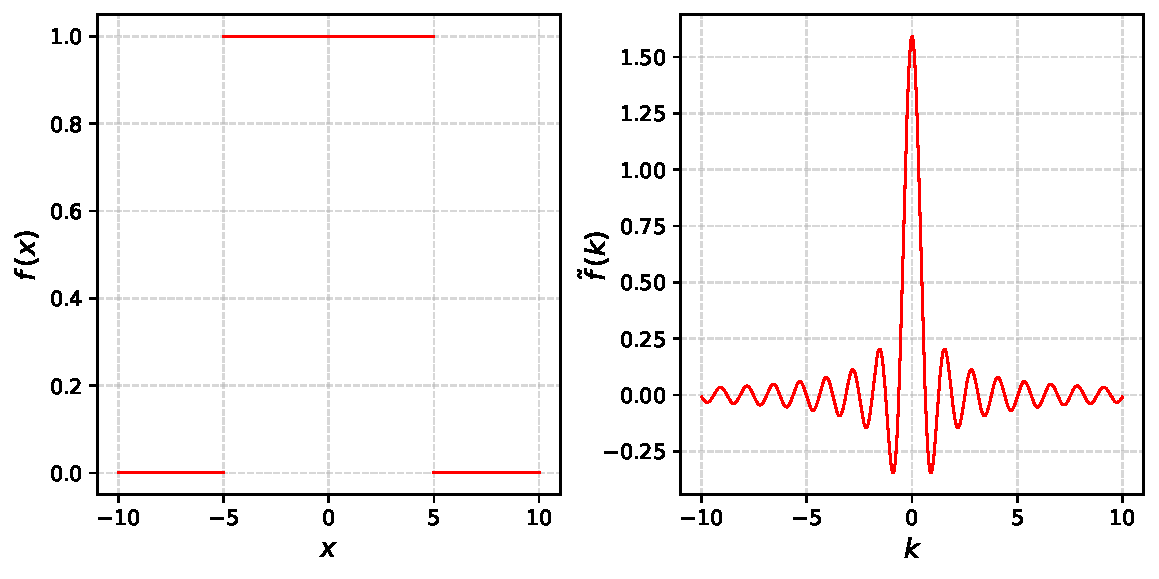
\includegraphics[scale = 0.55]{Figuras/EjemploTransformada1.pdf}
        \caption{Pulso cuadrado y su transformada de Fourier, con $a = 5$.}
        \label{Espectro2}
    \end{figure}

\end{ejemplo}

\begin{ejemplo}
    \textbf{Distribución gaussiana.} Considere la gaussiana
    \begin{equation*}
        f(x) = n e^{-\beta x^2}, \quad  \beta > 0 \ .
    \end{equation*}
    Su transformada de Fourier está dada por 
    \begin{equation*}
        \tilde{f}(k) =  \frac{n}{\sqrt{2\pi}} \int_{-\infty}^{\infty} e^{-\beta x^2} e^{-ikx} dx =  \frac{n}{\sqrt{2\pi}} \int_{-\infty}^{\infty} e^{-\beta x^2-ikx} dx .
    \end{equation*}

    Notemos que 
    \begin{align*}
        -\beta x^2-ikx &= - \beta \left( x^2 + \frac{ik}{\beta}x \right) \\
        &= - \beta \left( x^2 + \frac{ik}{\beta} x + \left( \frac{ik}{2\beta} \right)^2 - \left( \frac{ik}{2\beta} \right)^2 \right) \\
        &= - \beta \left( x + \frac{ik}{2\beta} \right)^2 + \beta \left( \frac{ik}{2\beta} \right)^2 \\
        &= - \beta \left( x + \frac{ik}{2\beta} \right)^2 - \left( \frac{k^2}{4\beta} \right).
    \end{align*}

    Luego, su transformada de Fourier puede escribirse como
    \begin{equation*}
        \tilde{f}(k) =  \frac{n}{\sqrt{2\pi}} \int_{-\infty}^{\infty} e^{-\beta \left( x + ik/2\beta \right)^2 - \left(k^2/4\beta \right)}  dx = \frac{n}{\sqrt{2\pi}} e^{- \left( k^2/4\beta \right)} \int_{-\infty}^{\infty} e^{-\beta \left( x + ik/2\beta \right)^2} \,dx. 
    \end{equation*}

    Haciendo el cambio de variable $u = x + \frac{ik}{2\beta}$, obtenemos que \footnote{}
    \begin{equation}\label{eq:Fourier-Gaussiana}
        \hat{f}(k) = \frac{n}{\sqrt{2\pi}} e^{- \left( k^2/4\beta \right)} \int_{-\infty}^{\infty} e^{-\beta u^2} \, du = \frac{n}{\sqrt{2\beta}} e^{- \left( k^2/4\beta \right)} \ ,
    \end{equation}
    donde hemos usado que 
    \begin{equation}
    \int_{-\infty}^{\infty} e^{-\beta x^2} \,dx = \sqrt{\frac{\pi}{\beta}}, \quad \beta > 0 \ . 
    \end{equation} 

    \begin{figure}[H]
        \centering
        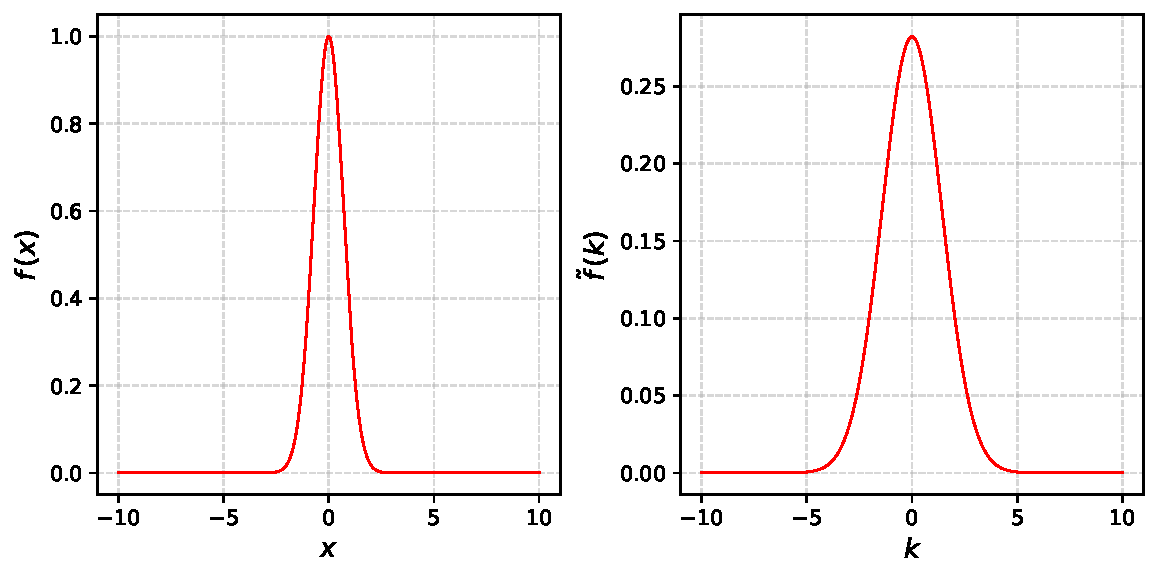
\includegraphics[width = 0.8\textwidth]{Figuras/EjemploTransformada2.pdf}
        \caption{Distribución gaussiana y su transformada de Fourier para $n=1$ y $\beta =1$ .}
        \label{Espectro3}
    \end{figure}
        \footnoterule
        
        {\footnotesize
        $^2$ En estricto rigor se debería calcular una integral compleja, vea \cite{Arfken}.
        }



    \begin{figure}[H]
        \centering
        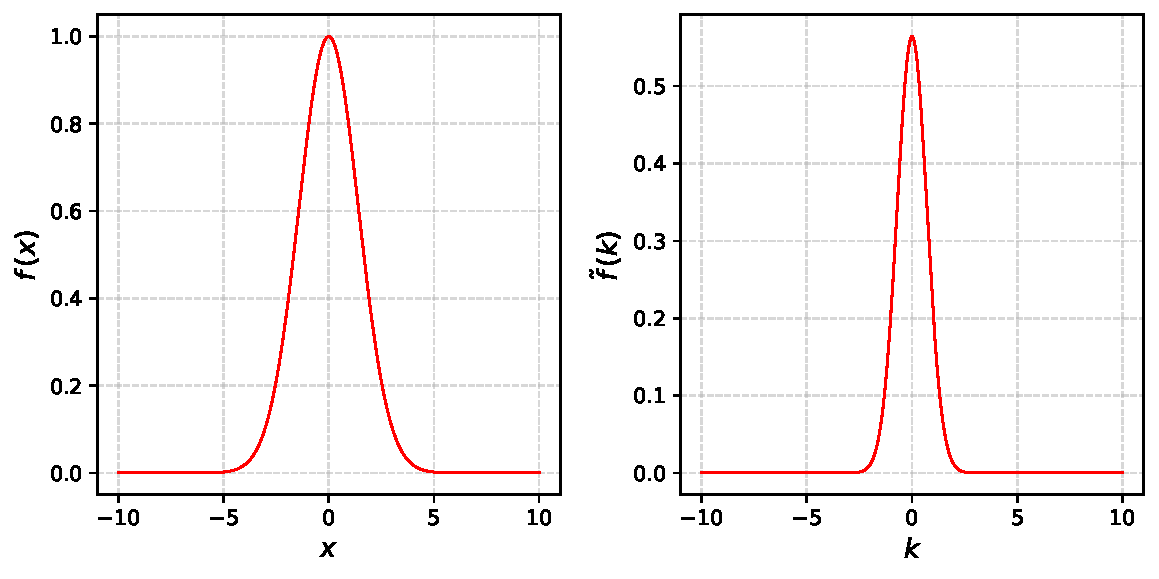
\includegraphics[scale = 0.6]{Figuras/EjemploTransformada3.pdf}
        \caption{Distribución gaussiana y su transformada de Fourier para $n=1$ y $\beta =0.25$ .}
        \label{Espectro4}
    \end{figure}
\end{ejemplo}


\subsection{Propiedades de la transformada de Fourier}

\begin{propiedad} 
\textbf{Propiedades de la Transformada de Fourier.} Sean las funciones $f, g \in L^1$ y los escalares $\alpha, \beta \in \mathbb{C}$.

\begin{enumerate}
    \item \textbf{Linealidad}: $$\mathcal{F}\{\alpha f(x) + \beta g(x)\}(k) = \alpha \mathcal{F}\{f(x)\}(k) + \beta \mathcal{F}\{g(x)\}(k).$$ 
    
    \item Si $f$ es real, entonces 
    % $$\tilde{f}(-k) = \tilde{f}^\ast(k).$$
    $$ \mathcal{F}\{f(x)\}(-k) = (\mathcal{F}\{f(x)\}(k))^*.$$
    
    \item \textbf{Traslación}: $$\mathcal{F}\{f(x+a)\}(k) = e^{ika} \mathcal{F}\{f(x)\}(k), \quad a \in \mathbb{R}.$$
    
    \item \textbf{Cambio de escala:} $$\mathcal{F}\{f(\alpha x)\}(k) = \frac{1}{|\alpha|}\mathcal{F}\{f(x)\}\left(\frac{k}{ \alpha}\right), \quad\alpha \neq 0.$$
    
    \item  \textbf{Atenuación}: $$\mathcal{F}\{f(x)e^{-ax}\}(k) =  \mathcal{F}\{f(x)\}(k-ia), \quad a \in \mathbb{C}.$$
    
    \item Si $f$ es una función par, entonces $\tilde{f}$ es una función real.
    
    \item Si $f$ es una función impar, entonces $\tilde{f}$ es una función puramente imaginaria, es decir, $\tilde{f}(k) = - \tilde{f}(-k)$.

    % \item \textbf{Escalonamiento:} $$\mathcal{F}\{f(\alpha x)\}(k) = \frac{1}{|\alpha|}\mathcal{F}\{f(x)\}\left(\frac{k}{ \alpha}\right), \quad\alpha \neq 0.$$
\end{enumerate}
\end{propiedad}

\begin{demo}
Demostraremos los puntos desde el 1 hasta el 5, y volveremos más tarde a los puntos 6 y 7.

\begin{enumerate}
    \item Por la definición \eqref{T.Fourier} de la transformada de Fourier y usando el hecho de que las funciones son absolutamente convergentes, tenemos
    \begin{align*}
        \mathcal{F}\{\alpha f(x) + \beta g(x)\}(k) &= \frac{1}{\sqrt{2\pi}} \int_{-\infty}^{\infty} [\alpha f(x) + \beta g(x)] e^{-ikx} dx \\
        &= \frac{\alpha}{\sqrt{2\pi}} \int_{-\infty}^{\infty}  f(x) e^{-ikx} dx + \frac{\beta}{\sqrt{2\pi}} \int_{-\infty}^{\infty}  g(x) e^{-ikx} dx \\
        &= \alpha \mathcal{F}\{f(x)\}(k) + \beta \mathcal{F}\{g(x)\}(k).
    \end{align*}
    
    \item Por la definición \eqref{T.Fourier} de la transformada de Fourier y suponiendo que $f$ es real:
    \begin{align*}
        \mathcal{F}\{f(x)\}(-k) &= \frac{1}{\sqrt{2\pi}} \int_{-\infty}^{\infty}  f(x)  e^{-(-ikx)} dx  \\
        &= \frac{1}{\sqrt{2\pi}} \int_{-\infty}^{\infty}  f(x)  (e^{-ikx})^* dx  \\
        &= \frac{1}{\sqrt{2\pi}} \int_{-\infty}^{\infty}  [f(x)  e^{-ikx}]^* dx \\
        &= (\mathcal{F}\{f(x)\}(k))^*.
    \end{align*}

    \item Por la definición \eqref{T.Fourier} de la transformada de Fourier, se tiene que
    \begin{equation*}
        \mathcal{F}\{f(x+a)\}(k) = \frac{1}{\sqrt{2\pi}}\int_{-\infty}^\infty f(x+a) e^{-ikx} dx \ .
    \end{equation*}

    Al hacer la sustitución $s = x+a$, $ds = dx$, tenemos
    \begin{align*}
        \frac{1}{\sqrt{2\pi}} \int_{-\infty}^\infty f(x+a)e^{-ikx}dx & = \frac{1}{\sqrt{2\pi}} \int_{-\infty}^\infty f(s) e^{-ik(s-a)} ds \\
        & = \frac{1}{\sqrt{2\pi}} \int_{-\infty}^\infty f(s) e^{-iks+ika} ds \\
        & = e^{ika} \left(\frac{1}{\sqrt{2\pi}} \int_{-\infty}^\infty e^{-iks} ds \right) \\
        & = e^{ika} \mathcal{F}\{f(x)\} (k) \ .
    \end{align*}

    \item Por la definición \eqref{T.Fourier} de la transformada de Fourier, se tiene que
    \begin{equation*}
        \mathcal{F} \{ f(\alpha x) \}(k) = \frac{1}{\sqrt{2\pi}} \int_{-\infty}^\infty f(\alpha x)e^{-ikx} dx \ .
    \end{equation*}

    Supondremos $\alpha > 0$. Haciendo el cambio de variable $u = \alpha x$, $du = \alpha dx$, tenemos
    \begin{equation*}
        \frac{1}{\sqrt{2\pi}} \int_{-\infty}^\infty f(\alpha x) e^{-ikx} dx = \frac{1}{\alpha} \left(\frac{1}{\sqrt{2\pi}} \int_{-\infty}^\infty f(u) e^{-i(k/\alpha)u} du \right) = \frac{1}{\alpha} \mathcal{F}\{f(x)\} \left( \frac{k}{\alpha} \right) \ .
    \end{equation*}

    Ahora, si $\alpha < 0$, hacemos el mismo cambio de variable que antes, obteniendo
    \begin{align*}
        \frac{1}{\sqrt{2\pi}} \int_{-\infty}^\infty f(\alpha x)e^{-ikx} dx & = \frac{1}{\alpha} \left( \frac{1}{\sqrt{2\pi}} \int_{\infty}^{-\infty} f(u) e^{-i(k/\alpha)u} du \right) \\ 
        & = - \frac{1}{\alpha} \left(\frac{1}{\sqrt{2\pi}} \int_{-\infty}^\infty f(u) e^{-i(k/\alpha)u} du \right) \\
        & = - \frac{1}{\alpha} \mathcal{F}\{f(x)\} \left(\frac{k}{\alpha}\right) \ .
    \end{align*}

    Por lo tanto, concluimos que, para $\alpha \neq 0$, se tendrá que
    \begin{equation*}
        \mathcal{F}\{(\alpha x)\}(k) = \frac{1}{|\alpha|} \mathcal{F}\{f(x)\} \left( \frac{k}{\alpha} \right) \ .
    \end{equation*}

    \item Por la definición \eqref{T.Fourier} de la transformada de Fourier, se tiene que
    \begin{align*}
        \mathcal{F}\{ f(x)e^{-ax} \}(k) & = \frac{1}{\sqrt{2\pi}} \int_{-\infty}^\infty f(x) e^{-ax} e^{-ikx} dx \\
        & = \frac{1}{\sqrt{2\pi}} \int_{-\infty}^\infty f(x) e^{-ikx-ax} dx \\
        & = \frac{1}{\sqrt{2\pi}} \int_{-\infty}^\infty f(x) e^{-ikx+i^2ax} dx \\
        & = \frac{1}{\sqrt{2\pi}} \int_{-\infty}^\infty e^{-ix(k-ia)} dx \\
        & = \mathcal{F}\{f(x)\}(k-ia) \ .
    \end{align*}
\end{enumerate}
\end{demo}

\begin{propo}\marginnote{Transformada de Fourier de una derivada}
Sea $f(x)$ con transformada de Fourier $\mathcal{F}\{f(x)\}$ y $\lim\limits_{x \to \pm \infty} f(x) = 0$. Entonces, 
\begin{equation}
    \boxed{\mathcal{F}\{f'(x)\} = i k \mathcal{F}\{f(x)\}\ ,} 
\end{equation}
y en general, 
\begin{equation}
    \mathcal{F}\{f^{(n)} (x)\} = (i k)^n \mathcal{F}\{f(x)\} \ ,
\end{equation}
\end{propo}

\begin{demo}
Demostraremos el caso para la primera derivada, pues derivadas más altas se deducen a partir de este. Usando la definición \eqref{T.Fourier} de la transformada de Fourier, tenemos que 
\begin{align*}
    \mathcal{F}\{f'(x)\} &= \frac{1}{\sqrt{2\pi}} \int_{- \infty}^{\infty} f'(x) e^{-ikx} \,dx \\
    &= \frac{1}{\sqrt{2\pi}} \int_{- \infty}^{\infty} \left\{ \frac{d}{dx}\left[ f(x) e^{-ikx} \right]  - (-ik) f(x) e^{-ikx} \right\}\,dx \\
    &= \frac{1}{\sqrt{2\pi}} \left. f(x) e^{-ikx} \right|_{-\infty}^{\infty} + \frac{ik}{\sqrt{2\pi}} \int_{- \infty}^{\infty}  f(x) e^{-ikx} \,dx \\
    &=  ik \mathcal{F}\{f(x)\} + \left. f(x) e^{-ikx} \right|_{-\infty}^{\infty}.
\end{align*}

Como  $\lim\limits_{x \to \pm \infty} f(x) = 0$, obtenemos
$$\mathcal{F}\{f'(x)\} = i k \mathcal{F}\{f(x)\}.$$
\end{demo}

% En general,
% \begin{shaded}
% $$,$$    
% \end{shaded}


Dado que hemos entendido la transformada de Fourier como una extensión de las series de Fourier, como es el caso de que las condiciones de existencia de la transformada de Fourier son las mismas \emph{condiciones de Dirichlet} para la existencia de los coeficientes de Fourier. Por ello, esperaríamos una analogía a la fórmula de Parseval propia de las series de Fourier. Esta corresponde al siguiente teorema.

\begin{teorema}[de Parseval]
Si $f(x)$ y $g(x)$ son funciones reales y si $\tilde{f}(k)$ y $\tilde{g}(k)$ son sus correspondientes transformadas de Fourier, entonces

\begin{itemize}
    \item[(i)] (Primer teorema)
    $$\int_{-\infty}^{\infty} |\tilde{f}(k)|^2\, dk = \int_{-\infty}^{\infty} |f(x)|^2 \, dx. $$
    
    \item[(ii)] (Segundo teorema)
    $$\int_{-\infty}^{\infty} \tilde{f}(k) \tilde{g}(-k) \, dk = \int_{-\infty}^{\infty} f(x) g(x) \, dx. $$
    
\end{itemize}
\end{teorema}

\begin{demo}
Notemos que (i) es consecuencia de (ii) al tomar $g(x) = f(x)$ real tal que $f^*(x) = f(x)$ y $\tilde{g}(-k) = \tilde{f}^*(k)$. Luego, nos bastará demostrar el segundo teorema de Parseval.

Usando la definición \eqref{T.Fourier}, tenemos que 
$$\tilde{g}(-k) = \frac{1}{\sqrt{2\pi}} \int_{-\infty}^{\infty} g(x) e^{ikx} \,dx.$$

Luego, 
$$\int_{-\infty}^{\infty} \tilde{f}(k) \tilde{g}(-k) \,dk = \int_{-\infty}^{\infty} \tilde{f}(k) \,dk \int_{-\infty}^{\infty} \frac{1}{\sqrt{2\pi}} g(x) e^{ikx} \,dx.$$

Supongamos que podemos intercambiar el orden de integración, por ejemplo, al suponer que las integrales 
$$\int_{-\infty}^{\infty} \tilde{f}(k) e^{ikx} \,dk ~~\mbox{y}~~ \int_{-\infty}^{\infty} g(x) e^{ikx} \,dx$$
son absolutamente integrables. Entonces,
$$\int_{-\infty}^{\infty} \tilde{f}(k) \tilde{g}(-k) \,dk = \int_{-\infty}^{\infty} g(x) \left( \frac{1}{\sqrt{2\pi}} \int_{-\infty}^{\infty} \tilde{f}(k) e^{ikx} \,dk\right) \,dx.$$

Aplicando la transformada inversa de Fourier dada por \eqref{I.Fourier}, concluimos que
$$\int_{-\infty}^{\infty} \tilde{f}(k) \tilde{g}(-k) \,dk = \int_{-\infty}^{\infty} f(x) g(x)  \,dx.$$

\end{demo}

\begin{ejemplo}
    Use el teorema de Parseval para evaluar
    $$\int_{-\infty}^{\infty}  \frac{\sin^2(x)}{x^2} \,dx.$$

    \textbf{Solución:} Esta integral puede ser calculada usando el teorema del residuo. En nuestro caso, usaremos el primer teorema de Parseval, teniendo en cuenta el resultado de la transformada de Fourier del pulso cuadrado en el ejemplo \ref{PulsoCuadrado}. 

    Para $a = 1$ en la ecuación \eqref{TransPulsoCuadrado}, tenemos que
    $$\int_{- \infty}^{\infty} |\Tilde{f}(k)|^2 \,dk = \int_{- \infty}^{\infty} \frac{2}{\pi} \frac{\sin^2(k)}{k^2}  \,dk = \frac{2}{\pi} \int_{-\infty}^{\infty}  \frac{\sin^2(k)}{k^2} \,dk.$$

    Por el primer teorema de Parseval,
    \begin{align*}
        \int_{- \infty}^{\infty} |\Tilde{f}(k)|^2 \,dk &= \int_{-\infty}^{\infty} |f(x)|^2 \,dx \\
        \Rightarrow \frac{2}{\pi} \int_{-\infty}^{\infty}  \frac{\sin^2(k)}{k^2} &=  \int_{-1}^1 \,dx = 2 \ . 
    \end{align*}

Por lo tanto,
$$\int_{-\infty}^{\infty}  \frac{\sin^2(k)}{k^2} \,dk = \pi.$$
\end{ejemplo}

\subsection{Transformadas seno y coseno}

Dependiendo de la paridad de las funciones a las cuales le aplicamos una transformada de Fourier, es posible utilizar una forma \emph{abreviada} de transformada, de manera similar a lo que podemos hacer para una serie de Fourier.

Notemos que, dada una función real $f(x)$ impar, tenemos que
\begin{align*}
    \tilde{f}(k) & = \frac{1}{\sqrt{2\pi}} \int_{-\infty}^{\infty} f(x) e^{-ikx} dx \\
    & = \frac{1}{\sqrt{2\pi}}  \int_{-\infty}^0 f(x) e^{-ikx} \,dx + \frac{1}{\sqrt{2\pi}} \int_{0}^{\infty} f(x) e^{-ikx} \, dx \\
    & = -\frac{1}{\sqrt{2\pi}}  \int_{\infty}^0 f(-x) e^{ikx} \,dx + \frac{1}{\sqrt{2\pi}}  \int_{0}^{\infty} f(x) e^{-ikx} \, dx \ , \quad x \to -x \mbox{ en la integral 1} \ , \\
    & = -\frac{1}{\sqrt{2\pi}} \int_{0}^{\infty} f(x) e^{ikx} \,dx + \frac{1}{\sqrt{2\pi}}  \int_{0}^{\infty} f(x) e^{-ikx} \, dx \ , \quad f(-x) = -f(x) \ ,  \\
     &= -\frac{1}{\sqrt{2\pi}}  \int_{0}^{\infty} f(x) [e^{ikx} - e^{-ikx}  ] \, dx \ , \quad \int_a^b = - \int_b^a \ , \\
    & = -\frac{2i}{\sqrt{2\pi}}  \int_{0}^{\infty} f(x) \sin(kx) \,dx \\
    & = -i \left(\sqrt{\frac{2}{\pi}}  \int_{0}^{\infty} f(x) \sin(kx) \,dx \right) \ .
    %  \equiv - i  \tilde{f}_S(k),
\end{align*}

\begin{defi}\marginnote{Transformada seno de Fourier}
    Se define la \textbf{transformada seno de Fourier}, $\tilde{f}_S(k) = \mathcal{F}_S(k)$ como
    \begin{equation}
        \tilde{f}_S(x) = \sqrt{\frac{2}{\pi}} \int_0^\infty f(x) \sin(kx) dx \ ,
    \end{equation}
    cuya transformada inversa es dada por
    \begin{equation}
        f(x) = \mathcal{F}^{-1}_S\{\tilde{f}_S(k)\} = \sqrt{\frac{2}{\pi}} \int_0^\infty \tilde{f}_S(k) \sin(kx) dx \ .
    \end{equation}

    Dada una función $f(x)$ real e impar, su transformada de Fourier será puramente imaginaria, y puede obtenerse como
    \begin{equation*}
        \tilde{f}(k) = -i \tilde{f}_S(k) \ .
    \end{equation*}
\end{defi}

De forma análoga, dada una función $f(x)$ real y par, tenemos

\begin{align*}
    \tilde{f}(k) & = \frac{1}{\sqrt{2\pi}} \int_{-\infty}^{\infty} f(x) e^{-ikx} dx \\
    & = \frac{1}{\sqrt{2\pi}} \int_{-\infty}^0 f(x) e^{-ikx} \,dx + \frac{1}{\sqrt{2\pi}} \int_{0}^{\infty} f(x) e^{-ikx} \, dx  \\
    & = -\frac{1}{\sqrt{2\pi}} \int_{\infty}^0 f(-x) e^{ikx} \,dx + \frac{1}{\sqrt{2\pi}} \int_{0}^{\infty} f(x) e^{-ikx} \, dx \ , \quad x \to -x \mbox{ en la integral 1} \ , \\
    & = \frac{1}{\sqrt{2\pi}} \int_{0}^{\infty} f(x) e^{ikx} \,dx + \frac{1}{\sqrt{2\pi}} \int_{0}^{\infty} f(x) e^{-ikx} \, dx \ , \quad f(-x) = f(x) \ , \\
    & = \frac{1}{\sqrt{2\pi}} \int_{0}^{\infty} f(x) [e^{ikx} + e^{-ikx}  ] \,dx \\
    & = \sqrt{\frac{2}{\pi}} \int_{0}^{\infty} f(x) \cos(kx) \,dx \ .
\end{align*}

\begin{defi}\marginnote{Transformada coseno de Fourier}
    Se define la \textbf{transformada coseno de Fourier}, $\tilde{f}_C(k) = \mathcal{F}_C(k)$ como
    \begin{equation}
        \tilde{f}_C(x) = \sqrt{\frac{2}{\pi}} \int_0^\infty f(x) \cos(kx) dx \ ,
    \end{equation}
    cuya transformada inversa es dada por
    \begin{equation}
        f(x) = \mathcal{F}^{-1}_C\{\tilde{f}_C(k)\} = \sqrt{\frac{2}{\pi}} \int_0^\infty \tilde{f}_C(k) \cos(kx) dx \ .
    \end{equation}

    Dada una función $f(x)$ real y par, su transformada de Fourier será real, y puede obtenerse como
    \begin{equation*}
        \tilde{f}(k) = \tilde{f}_C(k) \ .
    \end{equation*}
\end{defi}

Nuevamente, la elección del factor $\sqrt{\frac{2}{\pi}}$ es convencional, y otras elecciones pudieron ser hechas, mientras se satisfaga la integral de Fourier \eqref{IntegralFourier}.

% \begin{ejemplo}[Paridad]
% Si $f(x) \in \mathbb{R}$ e impar, entonces
% \begin{align*}
%      \tilde{f}(k) &= \frac{1}{2\pi} \int_{-\infty}^{\infty} f(x) e^{-ikx} dx \\
% &= \frac{1}{2\pi} \int_{-\infty}^0 f(x) e^{-ikx} \,dx + \frac{1}{2\pi} \int_{0}^{\infty} f(x) e^{-ikx} \, dx  \\
%  &= -\frac{1}{2\pi} \int_{\infty}^0 f(-x) e^{ikx} \,dx + \frac{1}{2\pi} \int_{0}^{\infty} f(x) e^{-ikx} \, dx \\
%      &= -\frac{1}{2\pi} \int_{0}^{\infty} f(x) e^{ikx} \,dx + \frac{1}{2\pi} \int_{0}^{\infty} f(x) e^{-ikx} \, dx  \\
%       &= -\frac{1}{2\pi} \int_{0}^{\infty} f(x) [e^{ikx} - e^{-ikx}  ] \,dx \\
%      &= -\frac{2i}{2\pi} \int_{0}^{\infty} f(x) \sin(kx) \,dx \equiv - i  \tilde{f}_S(k),
%      \end{align*}
     
%      donde $\tilde{f}_S$ es conocida como la \textbf{transformada seno de Fourier} de la función $f(x)$, y viene definida por \cite{Mauch} 
%      $$\boxed{\tilde{f}_S(k) = \frac{1}{\pi}  \int_{0}^{\infty} f(x) \sin(kx) \,dx}$$
     
% Análogamente a la definición de la  transformada seno de Fourier, si $f(x) \in \mathbb{R}$ y par, entonces 
% \begin{align*}
%      \tilde{f}(k) = \frac{1}{2\pi} \int_{-\infty}^{\infty} f(x) e^{-ikx} dx &= \frac{1}{2\pi} \int_{-\infty}^0 f(x) e^{-ikx} \,dx + \frac{1}{2\pi} \int_{0}^{\infty} f(x) e^{-ikx} \, dx  \\
%      &= -\frac{1}{2\pi} \int_{\infty}^0 f(-x) e^{ikx} \,dx + \frac{1}{2\pi} \int_{0}^{\infty} f(x) e^{-ikx} \, dx \\
%      &= \frac{1}{2\pi} \int_{0}^{\infty} f(x) e^{ikx} \,dx + \frac{1}{2\pi} \int_{0}^{\infty} f(x) e^{-ikx} \, dx \\
%      &= \frac{1}{2\pi} \int_{0}^{\infty} f(x) [e^{ikx} + e^{-ikx}  ] \,dx \\
%      &= \frac{2}{2\pi} \int_{0}^{\infty} f(x) \cos(kx) \,dx \equiv  \tilde{f}_C(k),
%      \end{align*}
     
% donde $\tilde{f}_C$ es conocida como la \textbf{transformada coseno de Fourier} de la función $f(x)$, y viene definida por \cite{Mauch}
%      $$\boxed{\tilde{f}_C(k) = \frac{1}{\pi}  \int_{0}^{\infty} f(x) \cos(kx) \,dx}$$

% \textbf{Observación: } Esta forma de escribir la transformada seno y coseno de Fourier es convencional, por el factor $1/\pi$.
% \end{ejemplo}

\subsection{Delta de Dirac}

Es común en física utilizar el concepto de \emph{pulso con duración infinitamente corta}. Por ejemplo, un cuerpo en movimiento por un golpe repentino alcanza un momentum igual al impulso del golpe, matemáticamente,
\begin{equation*}
    mv = I = \int_{t_0}^{t_0+\tau} F(t) dt \ ,
\end{equation*}
donde $F(t)$ es la fuerza y $\tau$ es la duracción de la acción de la fuerza. Al referirnos a un \emph{golpe}, insinuamos que la duración es lo suficientemente pequeña como para que el cambio en el momentum sea casi instantáneo. Sin embargo, para que esto sea posible, la fuerza debería haber sido infinita durante el golpe, y cero en otros lados.

Sin embargo, lo más probable es que la función se parezca a la figura X, donde $h$ es muy grande y $\tau$ muy pequeño, tal que el área debajo de la curva corresponde al impulso $I$. Para esto, necesitaríamos conocer la forma exacta de $F(t)$, lo que no siempre es posible. Para resolver este problema, aproximamos un pulso de esta forma por la \emph{`función'\footnote{Existe toda una discusión respecto al hecho de que este elemento no es una función propiamente dicha. Esta será omitida durante el curso.} Delta de Dirac}, que será de gran utilidad en diferentes áreas de la Física.

\begin{defi}\marginnote{Delta de Dirac}
    Se define la \textbf{Delta de Dirac} centrada en $x=a$ como la función
    \begin{equation}
        \delta(x-a) = \left\{ \begin{array}{cc}
            0 \ , & \quad x \neq a \ , \\
            \infty \ , & \quad x = a \ ,
        \end{array} \right.
    \end{equation}
    tal que la integral de $\delta(x)$ está normalizada,
    \begin{equation}
        \int_{-\infty}^{\infty} \delta(x-a) dx = 1 \ ,
    \end{equation}
    y que para cualquier función $f(x)$ continua, satisface
    \begin{equation}
        \int_{-\infty}^{\infty} \delta(x-a) f(x) dx = f(a) \ .
    \end{equation}
\end{defi}

\begin{propiedad}
    \textbf{Propiedades de la Delta de Dirac.}
    \begin{enumerate}
        \item Si $\delta'(x)$ denota a la derivada de la delta de Dirac, y $f'(x)$ representa la derivada de $f(x)$, entonces se satisface
        \begin{equation}
            \int_{-\infty}^{\infty} \delta'(x) f(x) \, dx = - f'(0) \ .
        \end{equation}

        Esta idea se puede generalizar a derivadas de orden superior, tal que, asumiendo que $f$ es $m$ veces diferenciable
        \begin{equation}
            \int_{-\infty}^{\infty} \delta^{(m)}(x) f(x) \, dx = - f^{(m)}(0) \ .
        \end{equation}

        \item Dada la \textbf{función escalón de Heaviside}, definida como
        \begin{equation}
            H(x) = \begin{array}{cc}
                0 \ , & x < 0 \ , \\
                1 \ , & x \geq 0 \ ,
            \end{array}
        \end{equation}
        entonces la delta de Dirac puede entenderse como su derivada, es decir,
        \begin{equation}
            \delta(x) = \frac{dH}{dx} \ .
        \end{equation}
        
        \item Dada una función continua $\phi(x)$, la delta de Dirac satisface
        \begin{equation}
            \phi(x+a) \delta(x) = \phi(a) \delta(x) \ ,
        \end{equation}
        y en particular,
        \begin{equation}
            x \delta(x) = 0 \ .
        \end{equation}
        \item A partir de las reglas de cambio de variables, podemos obtener que
        \begin{equation}
            \delta(g(x)) = \sum_i \frac{\delta(x-x_i)}{|g'(x_i)|} \ ,
        \end{equation}
        donde $x_i$ son las raíces de la función $g$, es decir, $g(x_i) = 0$, y que además satisfacen $g'(x_i) \neq 0$, para todo $x_i$.
        \item Como caso particular de la propiedad anterior, tenemos que
        \begin{equation}
            \delta(ax) = \frac{1}{|a|}\delta(x) \ , \qquad a \neq 0 \ .
        \end{equation}
        Como consecuencia,
        \begin{equation}
            \delta(-x) = \delta(x) \ .
        \end{equation}
    \end{enumerate}
\end{propiedad}

\subsection{Representación integral}

La delta de Dirac puede ser representada como
\begin{equation} \label{eq:Dirac-Integral}
    \delta(x-a) = \frac{1}{2\pi} \int_{-\infty}^{\infty} e^{ik(x-a)} dk \ .
\end{equation}

Podemos observar que esta definición es similar a la transformada de Fourier inversa de $e^{-ika}$. En efecto, utilizando la definición de la delta de Dirac, tenemos que
\begin{equation}
    \tilde{f}(k) = \frac{1}{\sqrt{2\pi}} \int_{-\infty}^\infty \delta(x-a) e^{-ikx} dx = \frac{1}{\sqrt{2\pi}} e^{-ika} \ .
\end{equation}

\begin{ejemplo}
    Determine la transformada de Fourier de las funciones $\sin(\alpha x)$ y $\cos(\alpha x)$.

    Observamos que, para $f(x) = \sin(\alpha x)$, tendremos
    \begin{align*}
        \mathcal{F}\{\sin(\alpha x)\}(k) & = \frac{1}{\sqrt{2\pi}} \int_{-\infty}^\infty \sin(\alpha x) e^{-ikx} dx \\
        & = \frac{1}{\sqrt{2\pi}} \int_{-\infty}^\infty \left( \frac{e^{i\alpha x} - e^{-i\alpha x}}{2i} \right) e^{-ikx} dx \\
        & = \frac{1}{2i} \left\{ \frac{1}{\sqrt{2\pi}} \int_{-\infty}^\infty e^{i(\alpha - k)x} dx - \frac{1}{\sqrt{2\pi}} \int_{-\infty}^\infty e^{-i(\alpha+k)x} dx \right\} \\
        & = \frac{1}{2i} \left\{ \sqrt{2\pi} \delta(\alpha-k) - \sqrt{2\pi} \delta(\alpha+k) \right\} \ , 
    \end{align*}
    donde hemos usado la definición de la delta de Dirac \eqref{eq:Dirac-Integral}. Luego,
    \begin{equation}
        \boxed{\mathcal{F}\{\sin(\alpha x)\}(k) = \sqrt{\frac{\pi}{2}}i[\delta(k+\alpha) - \delta(k-\alpha)] \ .}
    \end{equation}

    De forma análoga, para $f(x) = \cos(\alpha x)$, tendremos
    \begin{align*}
        \mathcal{F}\{\cos(\alpha x)\}(k) & = \frac{1}{\sqrt{2\pi}} \int_{-\infty}^\infty \cos(\alpha x) e^{-ikx} dx \\
        & = \frac{1}{\sqrt{2\pi}} \int_{-\infty}^\infty \left( \frac{e^{i\alpha x} + e^{-i\alpha x}}{2} \right) e^{-ikx} dx \\
        & = \frac{1}{2} \left\{ \frac{1}{\sqrt{2\pi}} \int_{-\infty}^\infty e^{i(\alpha - k)x} dx + \frac{1}{\sqrt{2\pi}} \int_{-\infty}^\infty e^{-i(\alpha+k)x} dx \right\} \\
        & = \frac{1}{2} \left\{ \sqrt{2\pi} \delta(\alpha-k) + \sqrt{2\pi} \delta(\alpha+k) \right\} \ , 
    \end{align*}
    donde hemos usado la definición de la delta de Dirac \eqref{eq:Dirac-Integral}. Luego,
    \begin{equation}
        \boxed{\mathcal{F}\{\cos(\alpha x)\}(k) = \sqrt{\frac{\pi}{2}}[\delta(k+\alpha) + \delta(k-\alpha)] \ .}
    \end{equation}

\end{ejemplo}

\subsection{Delta de Dirac tridimensional}

Por último, mencionaremos que es común en Física utilizar una delta de Dirac en tres (o más) dimensiones para describir distribuciones puntuales en el espacio, como lo puede ser una carga eléctrica puntual. Para ello, utilizamos una definición análoga al caso unidimensional, donde
\begin{equation}
    \delta^{(3)}(\vec{x}-\vec{a}) = 0 \, \quad \vec{x} \neq \vec{a} \ ,
\end{equation}
donde $\vec{x} = x \hat{x} + y \hat{y} + z\hat{z}$ es el vector posición de nuestro sistema coordenado, y $\vec{a} = a_x \hat{x} + a_y \hat{y} + a_z \hat{z}$ es un vector cualquiera que localiza a nuestro punto en el espacio. Para cualquier campo escalar, se cumplirá queda
\begin{equation}
    \int_V \delta^{(3)} (\vec{x}-\vec{a}) f(\vec{x}) dV = \left\{\begin{array}{cc}
        f(\vec{a}) \ , & \text{si } \vec{a} \in V \ , \\
        0 \ , & \text{si } \vec{a} \notin V \ .
    \end{array}\right.
\end{equation}

En coordenadas cartesianas, esta corresponde únicamente al producto de tres deltas de Dirac unidimensionales, una por cada coordenada del sistema, tal que
\begin{equation}
    \delta^{(3)}(\vec{x} - \vec{a}) = \delta(x-a_x) \delta(y - a_y) \delta(z - a_z) \ ,
\end{equation}
mientras que en un sistema de coordenadas curvilíneas ortogonales, cuyas coordenadas son $(\xi_1, \xi_2, \xi_3)$, y factores de escala 
\begin{equation}
    h_i = \left\| \frac{\partial \vec{x}}{\partial \xi_i} \right\| = \left[ \left( \frac{\partial x}{\partial \xi_i} \right)^2 + \left( \frac{\partial y}{\partial \xi_i} \right)^2 + \left( \frac{\partial z}{\partial \xi_i} \right)^2 \right]^{1/2} \ , \quad i = 1, 2, 3 \ ,
\end{equation}
la delta de Dirac será dada por
\begin{equation}
    \delta^{(3)}(\vec{x}-\vec{x}_0) = \frac{1}{h_1 h_2 h_3} \delta(\xi_1 - \xi_{10}) \delta(\xi_2 - \xi_{20}) \delta(\xi_3 - \xi_{30}) \ .
\end{equation}

\begin{demo}
    Proponemos un ansatz de la forma
    \begin{equation*}
        \delta^{(3)} (\x-\x_0) = A(\xi_1, \xi_2, \xi_3) \delta(\xi_1 - \xi_{10}) \delta(\xi_2 - \xi_{20}) \delta(\xi_3 - \xi_{30}) \ ,
    \end{equation*}
    donde $A(\xi_1, \xi_2, \xi_3)$ es una función que depende de las coordenadas.

    Este ansatz deberá satisfacer la condición de normalización de la delta de Dirac, 
    \begin{align*}
        \int_{\mathbb{R}^3} \delta^{(3)} (\x - \x_0) dV & = \int A(\xi_1, \xi_2, \xi_3) \delta(\xi_1 - \xi_{10}) \delta(\xi_2 - \xi_{20}) \delta(\xi_3 - \xi_{30}) h_1 h_2 h_3 d\xi_1 d\xi_2 d\xi_3 \\ 
        & = A(\xi_{10}, \xi_{20}, \xi_{30}) h_1(\xi_{10}, \xi_{20}, \xi_{30}) h_2(\xi_{10}, \xi_{20}, \xi_{30}) h_3(\xi_{10}, \xi_{20}, \xi_{30}) \\
        & = 1 \ ,
    \end{align*}
    con lo que podemos proponer que $A(\xi_1, \xi_2, \xi_3) = (h_1 h_2 h_3)^{-1}$, con lo que la delta de Dirac en un sistema curvilíneo ortogonal arbitrario está dada por
    \begin{equation*}
        \delta^{(3)}(\vec{x}-\vec{x}_0) = \frac{1}{h_1 h_2 h_3} \delta(\xi_1 - \xi_{10}) \delta(\xi_2 - \xi_{20}) \delta(\xi_3 - \xi_{30}) \ .
    \end{equation*}
\end{demo}

En particular, para \textbf{coordenadas esféricas}, la delta de Dirac es dada por
\begin{equation}
    \boxed{\delta^{(3)}(\vec{x} - \vec{x}_0) = \frac{1}{r^2 \sin\theta} \delta(r-r_0) \delta(\theta-\theta_0) \delta(\phi - \phi_0) \ ,}
\end{equation}
mientras que en \textbf{coordenadas cilíndricas}, será dada por
\begin{equation}
    \boxed{\delta^{(3)}(\x - \x_0) = \frac{1}{\rho} \delta(\rho - \rho_0) \delta(\phi-\phi_0) \delta(z-z_0) \ .}
\end{equation}

Mención aparte merece el caso en que el problema tiene simetría azimutal o axial. De acuerdo con la propiedad de normalización, $\int_V \delta^{(3)}(\vec{x}-\x_0) = 1$. Si omitimos la existencia de la delta en la coordenada azimutal $\phi$, esta integral se cumplirá únicamente si definimos la delta como
\begin{align*}
    \delta^{(3)}(\x - \x_0) & = \frac{1}{2\pi} \left( \frac{1}{r^2\sin\theta} \delta(r-r_0) \delta(\theta-\theta_0) \right) \ ,
    & = \frac{1}{2\pi} \left( \frac{1}{\rho} \delta(\rho - \rho_0) \delta(z-z_0) \right) \ ,
\end{align*}
ya que la integral de normalización incluirá un término de la forma
\begin{align*}
    \int_0^{2\pi} r^2 \sin \theta d\phi & = 2\pi r^2 \sin \theta \ , \\
    \int_0^{2\pi} \rho d\phi & = 2\pi \rho \ .
\end{align*}

Si en el caso esférico tenemos simetría axial, entonces
\begin{align*}
    \delta^{(3)}(\x - \x_0) = \frac{1}{2r^2} \delta(r - r_0) \delta(\phi - \phi_0) \ ,
\end{align*}
ya que
\begin{equation*}
    \int_0^\pi r^2 \sin \theta d\theta = 2r^2 \ .
\end{equation*}

Por último, si tenemos tanto simetría axial como azimutal, entonces
\begin{align*}
    \delta^{(3)}(\x - \x_0) = \frac{1}{4\pi r^2} \delta(r - r_0) \ ,
\end{align*}
ya que
\begin{equation*}
    \int_0^{2\pi} d\phi \int_0^\pi r^2 \sin \theta d\theta = 4\pi r^2 \ .
\end{equation*}

\begin{ejemplo}
    Considere un anillo de carga $Q$ distribuida uniformemente y radio $a$ ubicado en el plano $xy$ con su centro en el origen. Encuentre la densidad volumétrica de carga en coordenadas cilíndricas y en coordenadas esféricas.

    Recordamos que una densidad de carga, integrada sobre la región de interés, debe corresponderse con la carga total del sistema, es decir,
    \begin{equation*}
        \int_V \rho(\x) dV = Q \ .
    \end{equation*}

    Además, para una carga puntual $Q$ situada en el punto $\x_0$, podemos describir su densidad como
    \begin{equation*}
        \rho(\x) = Q \delta^{(3)}(\x-\x_0) \ .
    \end{equation*}

    Usaremos un enfoque similar a aquel de la carga puntual, pero considerando que el anillo es un objeto en dos dimensiones. Dado que la carga se distribuye uniformemente sobre el anillo, podemos suponer que el sistema tiene simetría azimutal. Además, como se ubica en el plano $xy$, esto quiere decir que $z_0 = 0$, y que $\theta_0 = \pi/2$. De esta forma, la densidad de carga del sistema será dada por
    \begin{align*}
        \rho(\x) & = Q \frac{1}{2\pi \rho} \delta(\rho - a) \delta(z) \ , \\
        & = Q \frac{1}{2\pi r^2 \sin\theta} \delta(r-a) \delta(\theta - \pi/2) \ .
    \end{align*}
    
    Es directo comprobar que, en ambos casos,
    \begin{equation*}
        \int_V \rho(\x) = Q \ .
    \end{equation*}
\end{ejemplo}

\subsection{Convolución}

Imaginemos algún tipo de \emph{estímulo} físico, por ejemplo, una fuerza en el tiempo, $f(t)$. Consideremos que la respuesta a este estímulo puede ser modelada mediante la función $g(x,t) = g(x-t)$, como puede ser, por ejemplo, el movimiento de una partícula en la posición $x$ frente a esta fuerza. Si el sistema es \emph{lineal}, entonces la respuesta total en el punto $x$ al estímulo global $\{f(t) : t \in \mathbb{R} \}$ será la \emph{suma} de todas las contribuciones infinitesimales $[dt f(t)] g(x,t)$. Matemáticamente, a estas contribuciones las llamamos \textbf{convolución}.

\begin{defi}\marginnote{Convolución}
Sean $f(x)$ y $g(x)$ dos funciones reales, se define la operación \textbf{convolución} de dos funciones $f$ y $g$ como 
\begin{equation}
 (f*g)(x) := \int_{-\infty}^{\infty} f(y) g(x-y) \,dy.   \label{Convolucion}
\end{equation}

\end{defi}

% \textbf{Idea física:} Sea $f(t)$ algún \emph{estímulo} físico, como puede serlo una fuerza en el tiempo $t$, la densidad de carga en la posición $x$, etc. Sea $g(x,t) = g(x-t)$ la respuesta en $x$ a un estímulo en $t$. Si el sistema es \textit{lineal}, la respuesta total en el punto $x$ al estímulo global $\{f(t) : t \in \mathbb{R}\}$ será la "suma" de todas las contribuciones $[dt\, f(t)] g(x,t)$, que es la convolución $(f*g)(x)$. 

Si nuestro estímulo es el potencial electrostático debido a una densidad de carga $\rho(\Vec{x})$, nuestra respuesta total, que corresponde al potencial electrostático $\phi(\x)$, se puede escribir como
\begin{equation}
    \phi(\Vec{x}) = \int_{V} \frac{\rho(\Vec{x}\,')}{|\Vec{x} - \Vec{x}\,'|} \, dV' = \rho * f(\Vec{x}) \ ,
\end{equation}
donde  $f(\Vec{x}) = 1/|\Vec{x}|$.
\begin{figure}[htbp]
    \centering
    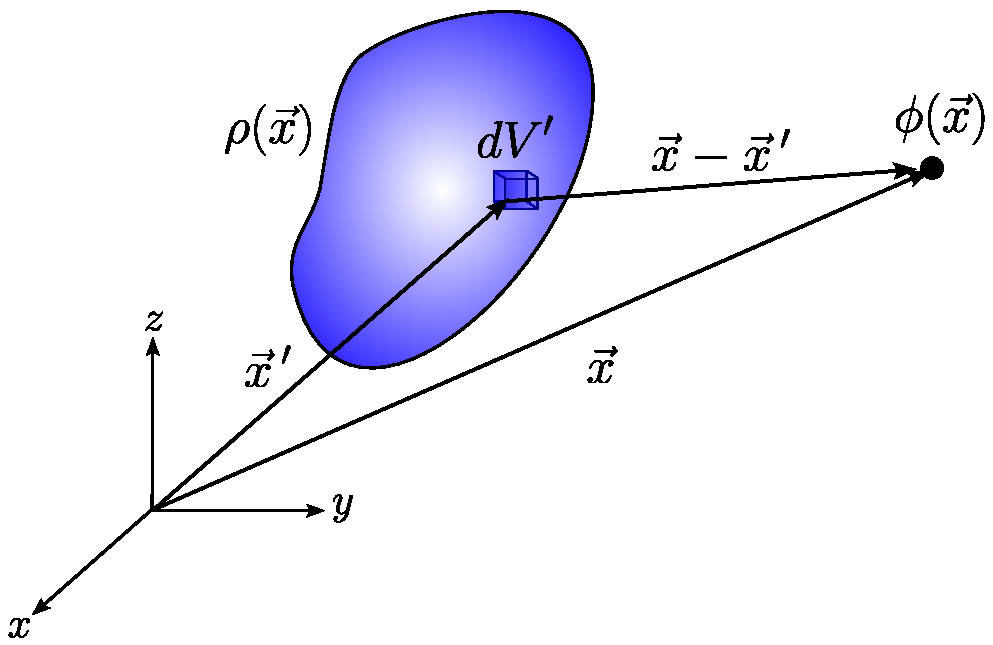
\includegraphics[width = 8cm]{Figuras/Distribucion-Cargas.pdf}
    \caption{Distribución de carga de densidad $\rho(\Vec{x})$.}
    \label{fig:PotencialDistribucion}
\end{figure}

Matemáticamente, podemos entender la convolución $f * g$ como \emph{el grado de traslape} entre dos pulsos, $f(y)$ y $g(-y)$, cuando uno $g(-y)$ se encuentra desplazado en $x$ unidades. Esta idea se puede observar en la figura \ref{fig:IdeaConvolucion}.

\begin{figure}[htbp]
    \centering
    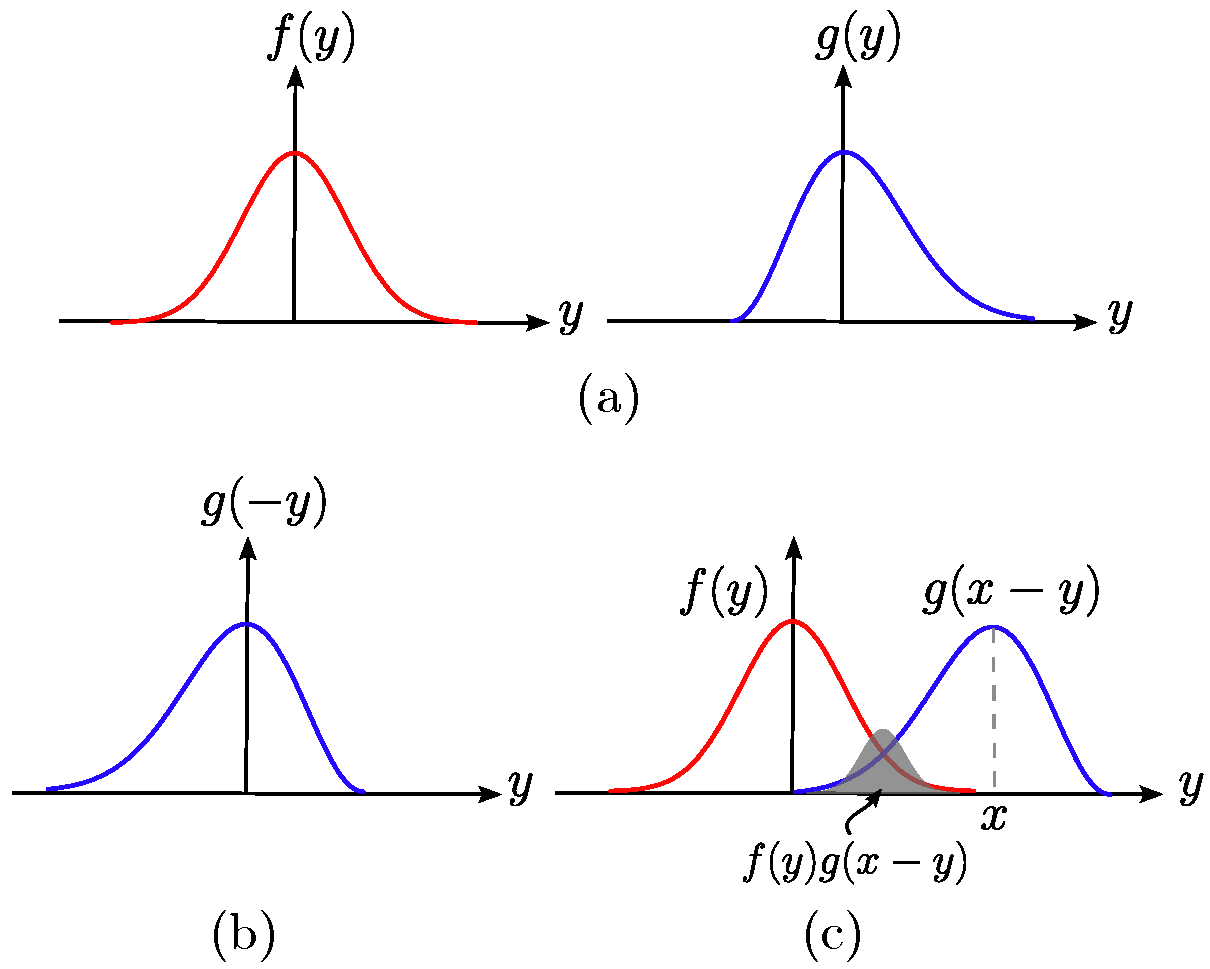
\includegraphics[width=10cm]{Figuras/Idea-Convolucion.pdf}
    \caption{Idea matemática de la convolución. En (a), se expresa cada función en términos de la variable de integración $y$. En (b), se refleja la gráfica de $g(y)$ con respecto al eje vertical, es decir, $g(y) \rightarrow g(-y)$. En (c), se traslada la gráfica de $g(-y)$, $x$ unidades. Luego, se traslapan las gráficas de $f(y)$ y $g(x-y)$ de tal forma que el área sombreada corresponde al valor de $f * g$ para ese valor de $x$.}
    \label{fig:IdeaConvolucion}
\end{figure}

% Entonces, $f * g$ mide el grado de traslape entre $f(y)$ y $g(-y)$, luego de trasladar $g$ a una distancia $x$.

\begin{propiedad}\textbf{Propiedades de la convolución.}

Sean $f(x)$, $g(x)$ y $h(x)$  funciones reales. Entonces, se verifican las siguientes propiedades:

\begin{enumerate}
    \item \textbf{Conmutatividad:}$$f(x) * g(x) = g(x) * f(x).$$
    
    \item \textbf{Asociatividad:} $$[f(x)*g(x)]*h(x) = f(x)*[g(x)*h(x)].$$
    
    \item \textbf{Distributividad:} $$f(x)*[g(x)+h(x)] = f(x)*g(x) + f(x)*h(x).$$ 
\end{enumerate}
\end{propiedad}

\newpage

\begin{teorema}[de convolución de Fourier]
Sean $f(x)$, $g(x)$ y $h(x)$  funciones reales y sean $\tilde{f}(k)$, $\tilde{g}(k)$ y $\tilde{h}(k)$ sus correspondientes transformadas de Fourier. 

\begin{itemize}
    \item Si $\tilde{h}(k) = \tilde{f}(k) \tilde{g}(k)$, entonces 
$$ h(x) = \frac{1}{\sqrt{2\pi}} (f * g)(x) = \frac{1}{\sqrt{2\pi}} \int_{-\infty}^{\infty} f(y) g(x-y) \,dy.$$ 

    \item Si $h(x) = f(x) g(x)$, entonces
    \begin{equation}
        \Tilde{h}(k) = \frac{1}{\sqrt{2\pi}}(\Tilde{f} * \Tilde{g})(k) = \frac{1}{\sqrt{2\pi}} \int_{-\infty}^{\infty} \Tilde{f}(y) \Tilde{g}(k-y) \,dy.
    \end{equation}
% $$$$
\end{itemize}
\end{teorema}

\begin{demo}
\ 

\begin{itemize}
    \item Supongamos que  $\tilde{h}(k) = \tilde{f}(k) \tilde{g}(k)$. Aplicando la transformada de Fourier inversa dada por \eqref{I.Fourier}, tenemos que 
\begin{align*}
   h(x) = \mathcal{F}^{-1} \{\tilde{h}(k)\} & = \mathcal{F}^{-1} \{\tilde{f}(k) \tilde{g}(k)\} \\
   & = \frac{1}{\sqrt{2\pi}} \int_{-\infty}^{\infty} \tilde{f}(k) \tilde{g}(k) e^{ikx} \,dk \\
   & = \frac{1}{\sqrt{2\pi}} \int_{-\infty}^{\infty}  \left( \frac{1}{\sqrt{2\pi}} \int_{-\infty}^{\infty} f(y) e^{-ik y} \,dy \right) \tilde{g}(k)  e^{ikx}  \,dk.
\end{align*}

Si el intercambio de orden de integración es posible, entonces 
\begin{align*}
  h(x) &= \frac{1}{\sqrt{2\pi}} \int_{-\infty}^{\infty}  f(y)  \left( \frac{1}{\sqrt{2\pi}} \int_{-\infty}^{\infty}  \tilde{g}(k)  e^{ikx} e^{-ik y}\,d k \right) \,dy \\
   & = \frac{1}{\sqrt{2\pi}} \int_{-\infty}^{\infty}  f(y)  \left( \frac{1}{\sqrt{2\pi}} \int_{-\infty}^{\infty}  \tilde{g}(k)  e^{ik(x-y)}\,d k \right) \,dy \\
   & = \frac{1}{\sqrt{2\pi}} \int_{-\infty}^{\infty}  f(y) g(x-y) \,dy = \frac{1}{\sqrt{2\pi}} (f * g)(x).
\end{align*}

Como la convolución es conmutativa:
$$h(x) = \frac{1}{2\pi} (f * g)(x) = \frac{1}{2\pi} (g * f)(x)  = \frac{1}{\sqrt{2\pi}} \int_{-\infty}^{\infty}  f(y) g(x-y) \,dy.$$

\item  Supongamos que $h(x) = f(x) g(x)$. Aplicando la transformada de Fourier dada por \eqref{T.Fourier}, tenemos que 
\begin{align*}
   \Tilde{h}(k) &=  \mathcal{F} \{f(x) g(x)\} \\
   &= \frac{1}{\sqrt{2\pi}} \int_{-\infty}^{\infty} f(x) g(x) e^{-ikx} \,dx \\
   &=  \frac{1}{\sqrt{2\pi}} \int_{-\infty}^{\infty} \left( \frac{1}{\sqrt{2\pi}} \int_{-\infty}^{\infty} \Tilde{f}(y) e^{iyx} \,dy \right) g(x) e^{-ikx} \,dx.
\end{align*}

Si el intercambio de orden de integración es posible, entonces 
\begin{align*}
   \Tilde{h}(k) &=  \frac{1}{\sqrt{2\pi}} \int_{-\infty}^{\infty} \Tilde{f}(y) \left( \frac{1}{\sqrt{2\pi}} \int_{-\infty}^{\infty} g(x) e^{iyx}  e^{-ikx}\,dx \right) \,dy \\
   &=  \frac{1}{\sqrt{2\pi}} \int_{-\infty}^{\infty} \Tilde{f}(y) \left( \frac{1}{\sqrt{2\pi}} \int_{-\infty}^{\infty} g(x) e^{-i(k-y)x} \,dx \right) \,dy \\
   &=  \frac{1}{\sqrt{2\pi}} \int_{-\infty}^{\infty} \Tilde{f}(y) \Tilde{g}(k-y) \,dy. 
\end{align*}

Por lo tanto,
$$\Tilde{h}(k) =  \frac{1}{\sqrt{2\pi}} (\Tilde{f} * \Tilde{g})(k) = \frac{1}{\sqrt{2\pi}} \int_{-\infty}^{\infty} \Tilde{f}(y) \Tilde{g}(k-y) \,dy.$$
\end{itemize}

\end{demo}


\begin{ejemplo}
    Sabiendo que \cite{Mauch}
    $$\mathcal{F}\left\{ \frac{2c}{x^2+c^2} \right\} = e^{-c|k|}, \quad \text{para} ~ c > 0.$$

    Podemos usar el teorema de convolución para encontrar la transformada de Fourier de
    \begin{equation}
      f(x) = \frac{1}{x^4+5x^2+4} = \frac{1}{(x^2+1)(x^2+4)}.    \label{EjConvo}
    \end{equation}
  
    En efecto,
    \begin{align*}
        \mathcal{F}\{f(x)\} &=  \mathcal{F}\left\{ \frac{1}{8} \frac{2}{x^2+1} \frac{4}{x^2+4} \right\} \\
        &= \frac{1}{8} \left( \int_{-\infty}^{\infty} e^{-|y|}e^{-2|k-y|} dy \right) \\
        &= \frac{1}{8} \left( \int_{-\infty}^0 e^{y}e^{-2|k-y|} dy +   \int_0^{\infty} e^{-y}e^{-2|k-y|} dy \right).
    \end{align*}

Si $k > 0$,
\begin{align*}
    \mathcal{F}\{f(x)\} &= \frac{1}{8} \left(  \int_{-\infty}^0 e^{y}e^{-2(k-y)} dy +  \int_0^k e^{-y}e^{-2(k-y)} dy + \int_k^{\infty} e^{-y}e^{2(k-y)} dy \right)  \\
    &= \frac{1}{8} \left(  \int_{-\infty}^0 e^{-2k+3y} dy +  \int_0^k e^{-2k+y} dy + \int_k^{+\infty} e^{2k-3y} dy \right) \\
    &= \frac{1}{8} \left( \frac{1}{3} e^{-2k} + e^{-k} - e^{-2k} + \frac{1}{3} e^{-k} \right) \\
    &= \frac{1}{6} e^{-k} - \frac{1}{12} e^{-2k}. 
\end{align*}

Si $k < 0$,
\begin{align*}
    \mathcal{F}\{f(x)\} &= \frac{1}{8} \left(  \int_{-\infty}^k e^{y}e^{-2(k-y)} dy +  \int_k^0 e^{y}e^{2(k-y)} dy + \int_0^{\infty} e^{-y}e^{2(k-y)} dy \right)  \\
    &= \frac{1}{8} \left(  \int_{-\infty}^k e^{-2k+3y} dy +  \int_k^0 e^{2k-y} dy + \int_0^{\infty} e^{2k-3y} dy \right) \\
    &= \frac{1}{8} \left( \frac{1}{3} e^{k} - e^{2k} + e^k + \frac{1}{3} e^{2k} \right) \\
    &= \frac{1}{6} e^{k} - \frac{1}{12} e^{2k}. 
\end{align*}

Por lo tanto, para $k$ positivo como negativo,
$$\boxed{\mathcal{F}\{f(x)\} =  \frac{1}{6} e^{-|k|} - \frac{1}{12} e^{-2|k|}} $$

Una mejor forma de encontrar la transformada de Fourier de \eqref{EjConvo} es, en primer lugar, descomponer la función en fracciones parciales,
$$f(x) = \frac{1}{3} \frac{1}{x^2+1} - \frac{1}{3} \frac{1}{x^2+4},$$

para luego hacer usar de la linealidad de la transformada.
\begin{align*}
     \mathcal{F}\{ f(x)\} &= \frac{1}{6} \mathcal{F} \left\{ \frac{2}{x^2+1}\right\} - \frac{1}{12} \mathcal{F} \left\{ \frac{4}{x^2+4} \right\}  \\
     &= \frac{1}{6} e^{-|k|} - \frac{1}{12} e^{-2|k|}.
\end{align*}

\end{ejemplo}

% \section{Aplicación de la transformada de Fourier}

% La transformada de Fourier es útil para resolver ecuaciones diferenciales en el dominio $(-\infty, \infty)$ con condiciones de borde homogéneas en el infinito. En particular, en ecuaciones diferenciales \underline{lineales} con \underline{coeficientes constantes}, debido a la propiedad de linealidad de la transformada.

% A continuación se ilustra el procedimiento a seguir mediante ejemplos.

% \begin{ejemplo}
%     Encuentre la solución general de la ecuación diferencial
%     $$y''(x) - y(x) = e^{-\alpha |x|}, \quad y(\pm \infty) = 0, \quad \alpha > 0, \alpha \neq 1.$$

%     \textbf{Solución:} La solución del caso homogéneo 
%     $$y''(x) - y(x) = 0,$$

%     está dada por
%     $$y_h(x) = c_1 e^{x} + c_2 e^{-x}, \quad c_1,c_2 \in \mathbb{R}.$$

%     Nos queda por encontrar la solución particular, para ello haremos uso de la transformada de Fourier. 

%     Primero, determinemos 
    
%     \begin{align*}
%         \mathcal{F}\left\{ e^{-\alpha |x|} \right\} &= \frac{1}{2\pi} \int_{-\infty}^{\infty} e^{-\alpha |x|} e^{-ikx} dx \\
%         &= \frac{1}{2\pi} \left(  \int_{-\infty}^{0} e^{x(\alpha -ikx)} dx +  \int_{0}^{\infty} e^{-x(\alpha + ik)} dx\right) \\
%         &= \frac{1}{2\pi} \left( \frac{1}{\alpha -ik} + \frac{1}{\alpha +ik} \right) \\
%         &= \frac{\alpha/\pi}{\alpha^2 + k^2}.
%     \end{align*}

%     Luego, apliquemos la transformada de Fourier a la ecuación diferencial:
%     \begin{align*}
%         \mathcal{F}\{ y''(x)\} - \mathcal{F}\{y(x)\ &=  \mathcal{F}\left\{ e^{-\alpha |x|} \right\} \\
%         \Rightarrow - k^2 \mathcal{F}\{y(x)\} - \mathcal{F}\{y(x)\} &= \frac{\alpha/\pi}{\alpha^2 + k^2}.
%     \end{align*}

%     Despejando la transformada de Fourier de la solución.
%     \begin{align*}
%         \mathcal{F}\{y(x)\} &= \frac{-\alpha/\pi}{(k^2 + \alpha^2)(k^2+1)} \\
%         &= - \frac{\alpha}{\pi} \frac{1}{\alpha^2-1} \left( \frac{1}{k^2+1} - \frac{1}{k^2+ \alpha^2}\right) \\
%         &= \frac{1}{\alpha^2-1} \left( \frac{\alpha/\pi}{k^2 + \alpha^2} - \alpha \frac{1/\pi}{k^2+1} \right.)
%     \end{align*}

%     Tomando la transformada inversa, obtenemos que
%     $$y(x) = \frac{e^{-\alpha|x| - \alpha e^{-|x|} }}{\alpha^2-1}.$$

%     Por lo tanto, la solución general es
%     $$\boxed{y(x) = \frac{e^{-\alpha|x| - \alpha e^{-|x|} }}{\alpha^2-1} + c_1 e^{x} + c_2 e^{-x}, \quad c_1,c_2 \in \mathbb{R}}$$
% \end{ejemplo}

% \begin{ejemplo}
%   Consideremos un oscilador armónico amortiguado sometido a una fuerza externa $g(t)$. La ecuación de movimiento del oscilador está dada por
% \begin{equation}
%  \ddot{x}(t) + 2 \alpha \dot{x}(t) + \omega_0^2 x(t) = f(t), \label{EDO-Oscilador}   
% \end{equation}

% donde $f(t) = g(t)/m$ y $\alpha$ es una constante asociada al amortiguamiento del sistema. En los primeros cursos de Ecuaciones Diferenciales Ordinarias (EDO) se trabaja con $f(t)$ sinusoidal, pero gracias a la transformada de Fourier, podemos extender este resultado para funciones $f(t)$ arbitrarias. 

% Aplicando la transformada de Fourier en la variable temporal, a saber,
% $$\mathcal{F}\{x(t)\} = \frac{1}{2\pi} \int_{-\infty}^{\infty} f(t) e^{-i\omega t} dt, $$

% a ambos lados de la ecuación diferencial \eqref{EDO-Oscilador}, obtenemos 
% \begin{align}
%     \mathcal{F}\left\{ \ddot{x}(t) + 2 \alpha \dot{x}(t) + \omega_0^2 x(t)\right\} &= \mathcal{F}\left\{ f(t)\right\} \nonumber\\
%     \Rightarrow   \mathcal{F}\left\{ \ddot{x}(t) \right\} + 2\alpha \mathcal{F}\left\{ \dot{x}(t) \right\} + \omega_0^2 \mathcal{F}\{x(t)\} &= \mathcal{F}\left\{ f(t)\right\}. \label{EDO-Transformada}
% \end{align}

% Si asumimos que 
% $$\lim_{x \to \pm \infty} x(t) = \lim_{x \to \pm \infty} \dot{x}(t) = 0,$$

% tenemos 
% \begin{align*}
%      \mathcal{F}\left\{ \ddot{x}(t) \right\} &= (i\omega)^2 \mathcal{F}\{x(t)\} = - \omega^2 \mathcal{F}\{x(t)\},\\
%       \mathcal{F}\left\{ \dot{x}(t) \right\} &= i \omega \mathcal{F}\{x(t)\}.
% \end{align*}

% Además, si definimos $F(\omega) := \mathcal{F}\left\{ f(t)\right\}$, la ecuación \eqref{EDO-Transformada} nos queda
% $$ - \omega^2 \mathcal{F}\{x(t)\} + 2 \alpha \omega i \mathcal{F}\{x(t)\} + \omega_0^2 \mathcal{F}\{x(t)\} = F(\omega).$$

% Despejando la transformada de Fourier de la solución:
% $$  \mathcal{F}\{x(t)\} = \frac{F(\omega)}{-\omega^2 - 2 \alpha i \omega + \omega_0^2}.$$

% Tomando la transformada inversa, obtenemos la solución 
% $$\boxed{x(t) = \int_{-\infty}^{\infty} \frac{F(\omega)}{(\omega_0^2-\omega^2) - 2 \alpha \omega i} e^{i\omega t} d\omega }$$  
% \end{ejemplo}


\section{Transformada de Laplace}

% \section{Definición}

\begin{defi}
Sea $f(t)$ una función a valores reales definida para $t \in [0, \infty[$. La \textbf{transformada de Laplace} de $f$ es la función $F$ definida mediante la integral impropia
$$F(s) := \int_0^{\infty} e^{-st} f(t) \,dt.$$

El dominio de $F(s)$ está formado por todos lo valores de $s$ (complejos) para los que la integral existe. Simbólicamente,
$$F(s) = \mathcal{L}\{f(t)\}.$$
\end{defi}

\begin{ejemplo}
Determine la transformada de Laplace de 
$$f(t) = e^{at}.$$

\textbf{Solución:} Por definición, 
\begin{align*}
    \mathcal{L}\{e^{at}\} = \int_0^{\infty} e^{-st} e^{at} \,dt &= \int_0^{\infty} e^{-(s-a)t} \,dt \\
    &= \left. - \frac{e^{-(s-a)t}}{s-a} \right|_0^{\infty} \\
    &= \frac{1}{s-a}, \quad \real(s) > a.
\end{align*}

En efecto, si hacemos $s = \real(s) + i \im(s)$, tenemos que
$$\lim_{t\to + \infty} \left| e^{-(s-a)t} \right| = \lim_{t\to + \infty} \left|e^{-(\real(s) - a)t} \right| = 0, \quad \real(s) > a. $$
\end{ejemplo}

\begin{ejemplo}
    Consideremos la transformada de Laplace de la \textbf{función de Heaviside},
    $$H(t-a) = \left\{ \begin{array}{cl}
     0,& \text{si} ~ t < a  \\
     1,& \text{si} ~ t > a
    \end{array} \right.,$$

    para un número real $a$ no negativo.
    \begin{align*}
        \mathcal{L}\{H(t-a)\} &= \int_0^{\infty} e^{-st} H(t-a) \,dt \\
        &= \int_a^{\infty} e^{-st} \,dt \\
        &= \left. - \frac{e^{-st}}{s}\right|_a^{\infty} \\
        &= \frac{e^{-as}}{s}, \quad \real(s) > 0.
    \end{align*}

    Ahora, consideremos $H(t-a)f(t-a)$.
    \begin{align*}
        \mathcal{L}\{H(t-a)f(t-a)\} &= \int_0^{\infty} e^{-st} H(t-a)f(t-a) \,dt \\
        &= \int_a^{\infty} e^{-st} f(t-a) \,dt \\
        &= \int_0^{\infty} e^{-s(t+a)} f(t) \,dt \\
        &= e^{-as} F(s).
    \end{align*}

\end{ejemplo}

\begin{ejemplo}
    Queda como ejercicio para el lector demostrar que
    \begin{align*}
        \mathcal{L}\{\cos(at)\} &= \frac{s}{s^2+a^2}, \quad \real(s) > 0, \\
        \mathcal{L}\{\sin(at)\} &= \frac{a}{s^2+a^2}, \quad \real(s) > 0.
    \end{align*}
\end{ejemplo}

En la mayoría de los casos será posible calcular $\mathcal{L}\{f(t)\}$ por evaluación directa. Sin embargo, no satisface la necesidad de determinar un conjunto razonable de condiciones que nos asegure la existencia de la transformada de Laplace de una función dada $f$.

A partir de la definición, es claro que $f$ debe escogerse de manera que
\begin{equation}
\int_0^{t_0} e^{-st} f(t) dt \label{Laplace1}
\end{equation}

exista para todo $t_0 > 0$. Ésto se logra exigiendo que $f$ sea seccionalmente continua en todo el intervalo $[0,t_0]$, con $t_0>0$. No obstante, no es suficiente para garantizar la existencia de $\mathcal{L}\{f(t)\}$ ya que al tomar el límite $t_0 \to \infty$ de \eqref{Laplace1}, ésta debe converger. A grandes rasgos, mostraremos que la transformada de Laplace de una función continua por partes existe, siempre que la función no crezca más rápido que una exponencial.

\begin{defi}
    Una función $f(t)$ es de \textbf{orden exponencial $\alpha$} en $[0,\infty[$ si existen constantes positivas $T$ y $M$ tales que
    $$\forall t \in [T, \infty[: ~ |f(t)| \leq M e^{\alpha t}.$$
\end{defi}

\begin{ejemplo}
\ 

    \begin{itemize}
        \item Toda función acotada es de orden exponencial 0.

        \item $t e^{2t}$ es de orden exponencial $\alpha$ para cualquier $\alpha > 2$. En efecto,
        $$\lim_{t \to \infty} \frac{t e^{2t}}{e^{\alpha t}} = \lim_{t \to \infty} \frac{t}{e^{(\alpha-2) t}} \overset{L'H}{=} \lim_{t \to \infty} \frac{1}{(\alpha -2 )e^{(\alpha-2) t}} = 0,$$

        para $\alpha > 2$. Eligiendo $M = 1$, por definición de límite, existe $T > 0$ tal que 
        $$\left|\frac{t e^{2t}}{e^{\alpha t}} \right| < 1 \Rightarrow |te^{2t}| < e^{\alpha t}, \quad \text{si} ~ t \geq T.$$
        
        \item $e^{t^2}$ no es de orden exponencial. En efecto,
        $$\lim_{t \to  \infty} \frac{e^{t^2}}{e^{\alpha t}} = \lim_{t \to \infty} e^{t(t-\alpha)} = \infty, \quad \mbox{para todo} ~ \alpha.$$

        Ésto es,
        $$(\forall M >0)(\exists T >0)\left(t \geq T \Rightarrow e^{t^2} > M e^{\alpha t}\right).$$

        \item $t^n, n \in \mathbb{N}$ es de orden exponencial $\alpha$ para cualquier $\alpha > 0$ (ejercicio para el lector).
    \end{itemize}
\end{ejemplo}

\begin{teorema}[de existencia] \label{ExistenciaLaplace}
Si $f$ es una función seccionalmente continua y de orden exponencial $\alpha$, entonces la transformada de Laplace
$$\mathcal{L}\{f(t)\} = \int_0^{\infty} e^{-st} f(t) \,dt$$

converge para $\real(s) > \alpha$. Más aún, la integral es absolutamente y uniformemente convergente para $\real(s) \geq \alpha_1 >  \alpha$.
\end{teorema}

\textbf{Observación:} Existen funciones que tienen transformada de Laplace y que no satisfacen las hipótesis del teorema. Por ejemplo, $f(t) = \frac{1}{\sqrt{t}}$ no es de orden exponencial, pues tiende a $\infty$ cuando $t \to 0^+$. Sin embargo,
\begin{equation*}
\mathcal{L}\{f(t)\} = \sqrt{\frac{\pi}{s}}.
\end{equation*}

En efecto, haciendo $x^2 = st$ y considerando que $\int_0^{\infty} e^{-x^2} dx = \frac{\sqrt{\pi}}{2}$, se tiene que
\begin{equation*}
\mathcal{L}\{t^{-1/2}\} = \int_0^{\infty} e^{-st}t^{-1/2}dt = \frac{2}{\sqrt{s}} \int_0^{\infty} e^{-x^2} dx = \sqrt{\frac{\pi}{s}}.
\end{equation*}

\begin{teorema}
    Bajo las mismas condiciones del teorema \ref{ExistenciaLaplace}, la transformada de Laplace $F(s)$ es holomorfa (analítica) en $\real(s) \geq \alpha_1 > \alpha$, es decir, la derivada $F'(s)$ existe en dicho semiplano.
\end{teorema}

En general, existe
\begin{shaded}
$$\frac{d^n}{ds^n} F(s) = (-1)^n \mathcal{L}\{t^n f(t)\}.$$
\end{shaded}

\begin{propo} \label{T.LaplaceLim}
Bajo las mismas condiciones del teorema \ref{ExistenciaLaplace},
$$\lim_{\real(s) \to \infty} F(s) = 0.$$
\end{propo}

\begin{demo}
    Si $f$ es de orden exponencial $\alpha$, entonces existen constantes  $T, M >0$ tales que
\begin{equation*}
|f(t)| \leq M e^{\alpha t}, \quad \forall t \geq T.
\end{equation*}

Luego,
\begin{eqnarray*}
\left|F(s)\right| = \left| \int_0^{+\infty} e^{-st} f(t) dt \right| &\leq &\left| \int_0^{T} e^{-st} f(t) dt \right| + \left| \int_T^{+\infty} e^{-st} f(t) dt \right| \\
& \leq & \int_0^T e^{-\real(s)t} |f(t)| dt +  \int_T^{+\infty} e^{-\real(s)t} |f(t)| dt \\
& \leq & I + \frac{M e^{-(\real(s)-\alpha)T}}{\real(s)-\alpha}, \quad \real(s) > \alpha
\end{eqnarray*}

donde $I = \int_0^T e^{-\real(s)t} |f(t)| dt$.

Como 
\begin{equation*}
\lim_{\real(s) \to +\infty} \left[ I + \frac{M e^{-(\real(s)-\alpha)T}}{\real(s) -\alpha} \right] = \cancelto{0}{\lim_{\real(s) \to +\infty} I} +  \cancelto{0}{\lim_{\real(s) \to +\infty} \frac{M e^{-(\real(s)-\alpha)T}}{\real(s) -\alpha}} = 0,
\end{equation*}

concluimos que
$$\lim_{s \to + \infty} F(s) = 0.$$
\end{demo}

\textbf{Observaciones:}

\begin{itemize}
\item[(a)] El contrarrecíproco del teorema es: si $\lim\limits_{s \to + \infty} \mathcal{L}\{f(t)\} \neq 0$, entonces no existe $f(t)$ tal que $F = \mathcal{L}\{f(t)\}$.

\item[(b)] Por observación $(a)$ podemos decir inmediatamente que funciones tales como $\frac{s+4}{s-1}, s, s^2, \sin(s)$, etc. no tienen transformada inversa de Laplace.
\end{itemize} 

\subsection{Transformada inversa de Laplace}

\begin{defi}
Dada una función $F(s)$, si existe una función $f(t)$ que sea continua en $[0, + \infty[$ y satisfaga
\begin{equation}
\mathcal{L}\{f(t)\} = F, \label{LaplaceInversa}
\end{equation}

entonces decimos que $f(t)$ es la \textbf{transformada inversa de Laplace} de $F(s)$ y utilizamos la notación $f = \mathcal{L}^{-1} \{F(s)\}$.
\end{defi}

Es natural preguntarse si la transformada inversa de Laplace es única, para ello basta con determinar si $\mathcal{L}$ es una aplicación inyectiva o no. El siguiente teorema (sin demostración) garantiza la inyectividad sin considerar los puntos de discontinuidad de las funciones.

\begin{teorema}[de Lerch]
 Sea $f$ y $g$ funciones continuas por tramos y de orden exponencial, y supongamos que existe un número real $s_0$ tal que
\begin{equation*}
\mathcal{L}\{f\}(s) = \mathcal{L}\{g\}(s), \quad \forall Re(s) >s_0.
\end{equation*}

Entonces, con la posible excepción de los puntos de discontinuidad, $f(t) = g(t)$ para todo $t >0$.
\end{teorema}

Por lo tanto, dos funciones continuas por tramos que satisfagan \eqref{LaplaceInversa}, sólo pueden diferir en sus puntos de discontinuidad. Luego, la completa unicidad se alcanza si se impone la continuidad a $f$.

Otra interrogante es: ¿es $\mathcal{L}$ un operador sobreyectivo?. La respuesta es no y viene avalada por el teorema \ref{T.LaplaceLim}.

La transformada inversa de Laplace puede ser calculada con la siguiente integral compleja conocida como la \textbf{fórmula de inversión de Mellin} o \textbf{integral de Bromwich} \cite{Arfken}.
\begin{shaded}
   $$ f(t) = \frac{1}{2\pi i} \int_{\gamma - i \infty}^{\gamma + i \infty} e^{st} F(s) \,ds,$$
\end{shaded}

donde $\gamma$ es una constante real que se encuentra a la derecha de las singularidades de $F(s)$.

\textbf{Observación:} Matemáticamente hablando, se debería escribir $$f(t) = \frac{1}{2\pi i} V.P. \int_{\gamma - i \infty}^{\gamma + i \infty} e^{st} F(s) \,ds,$$ 

pues 
$$f(t) = \frac{1}{2\pi i} \lim_{R \to \infty} \int_{L_R} e^{st} F(s) \,ds,$$ 

con $L_R: s = \gamma + it, - R\leq t \leq R$.

% \subsection*{Origen de la fórmula de inversión de Mellin*}

% Supondremos que $f(t)$ es de orden exponencial $\gamma$, entonces existen $T,M > 0$ tales que
% $$|f(t)| \leq M e^{\gamma t}, \quad \forall t \geq T,$$

% donde el número real $\gamma$ se escoge tal que la recta $x = \gamma$ esté a la derecha de todas las singularidades de $F(s)$.

% Por definición de la transformada de Laplace, se tiene que
% $$F(s) = \int_0^{\infty} e^{-su} f(u) \,du.$$

% Luego,
% $$\lim_{R \to \infty} \frac{1}{2\pi i} \int_{\gamma -i R}^{\gamma + i R} e^{st} F(s) \,ds = \lim_{R \to \infty} \frac{1}{2\pi i} \int_{\gamma -i R}^{\gamma + i R} \int_0^{\infty} e^{st-su} f(u) \,du \,ds.$$

% Evaluando la integral compleja, ésto es, $s = \gamma +i y$ y $ds = i dy$, con $- R\leq y \leq R$, obtenemos que
% \begin{align*}
%    \lim_{R \to \infty} \frac{1}{2\pi i} \int_{\gamma -i R}^{\gamma + i R} e^{st} F(s) \,ds &=  \lim_{R \to \infty} \frac{1}{2\pi i} \int_{- R}^{R} \int_0^{\infty} i e^{(\gamma + iy)t - (\gamma + i y)u} f(u) \,du \,dy \\
%    &= \lim_{R \to \infty} \frac{1}{2\pi} e^{\gamma t} \int_{- R}^{R} \int_0^{\infty} e^{i y t} e^{-\gamma u} e^{-iy u} f(u) \,du \,dy.
% \end{align*}

% Notemos que para $u \geq T$,
% $$| e^{i y t} e^{-\gamma u} e^{-iy u} f(u)| \leq e^{-\gamma u} |f(u)|.$$

% Por el teorema \ref{ExistenciaLaplace}, la integral de la transformada de Laplace $F(s)$ converge absolutamente, en específico para $s = \gamma$, luego
% $$\int_0^{\infty} |e^{-\gamma u} f(u)| \,du = \int_0^{\infty} e^{-\gamma u} |f(u)| \,du,$$

% converge. Así, usando el test de convergencia uniforme para integrales, la integral 
% $$\int_0^{\infty} e^{i y t} e^{-\gamma u} e^{-iy u} f(u) \,du $$

% converge uniformemente para $-R \leq y \leq R$. Luego, podemos intercambiar el orden de integración de acuerdo al teorema \ref{TeoA:OrdenIntegracion1} como sigue.
% \begin{align*}
%    \lim_{R \to \infty} \frac{1}{2\pi i} \int_{\gamma -i R}^{\gamma + i R} e^{st} F(s) \,ds &= \lim_{R \to \infty} \frac{1}{2\pi} e^{\gamma t} \int_{0}^{\infty} e^{-i y u} e^{-\gamma u} f(u) \left( \int_{-R}^R e^{i y t} dy \right) du \\
%    &=  \lim_{R \to \infty} \frac{1}{2\pi} e^{\gamma t}  \int_{-R}^R e^{iy t} dy  \int_{0}^{\infty} e^{-i y u} e^{-\gamma u} f(u) du \\
%    &= \frac{1}{2\pi} e^{\gamma t}  \int_{-\infty}^{\infty} e^{iyt} dy  \int_{0}^{\infty} e^{-i y u} [e^{-\gamma u} f(u)] du.
% \end{align*}

% Comparando con la ecuación \eqref{IntegralFourier}, podemos notar que 
% $$\int_{-\infty}^{\infty} e^{iy t} dy  \int_{0}^{\infty} e^{-i y u} [e^{-\gamma u} f(u)] du = \left\{ \begin{array}{cl}
%      2\pi e^{- \gamma t} f(t),& t > 0  \\
%      0,& t < 0
% \end{array} \right..$$

% Por lo tanto,
% $$  \lim_{R \to \infty} \frac{1}{2\pi i} \int_{\gamma -i R}^{\gamma + i R} e^{st} F(s) \,ds = f(t), \quad t > 0.$$

\subsection{\texorpdfstring{$F(s)$}{TEXT} con polos}

\begin{teorema}
    Si $F(s)$ es analítica excepto por las singularidades aisladas en $s_1, s_2, \dots, s_n$ y 
    $$\lim_{R \to \infty} \sup_{ |s - \gamma| = R} |F(s)| =  0.$$
   
   Entonces, la transformada de Laplace inversa de $F(s)$ es
    $$f(t) = \mathcal{L}^{-1}\{F(s)\} = \sum_{k= 1}^n Res(e^{st} F(s), s_k), \quad t > 0.$$
\end{teorema}

\begin{ejemplo}
    Determine la transformada inversa de Laplace de 
    $$F(s) = \frac{s^2}{s^4-1}.$$

    \textbf{Solución:} La transformada inversa de $F(s)$ está dada por la suma de los residuos de
    $$\psi(s) = e^{st} F(s) = e^{st} \frac{s^2}{(s-1)(s+1)(s-i)(s+i)}.$$

    Las singularidades de $\psi$ son $s = \pm 1, \pm i$, todos polos de orden 1. De esta manera, los residuos están dados por:
    \begin{align*}
        Res(\psi, 1) &= \lim_{s \to 1} (s-1) \psi(s) = \lim_{s\to 1} \left[e^{st} \frac{s^2}{(s+1)(s-i)(s+i)} \right] = \frac{e^t}{4},\\
        Res(\psi, -1) &= \lim_{s \to -1} (s+1) \psi(s) = \lim_{s\to -1} \left[e^{st} \frac{s^2}{(s-1)(s-i)(s+i)} \right] = -\frac{e^{-t}}{4}, \\
        Res(\psi, i) &= \lim_{s \to i} (s-i) \psi(s) = \lim_{s\to i} \left[e^{st} \frac{s^2}{(s-1)(s+1)(s+i)} \right] = \frac{e^{it}}{4i}, \\
        Res(\psi, -i) &= \lim_{s \to -i} (s+i) \psi(s) = \lim_{s\to -i} \left[e^{st} \frac{s^2}{(s-1)(s+1)(s-i)} \right] = -\frac{e^{-it}}{4i}.
    \end{align*}

    Por lo tanto,
    \begin{align*}
        \mathcal{L}^{-1} \left\{\frac{s^2}{s^4-1} \right\} &= Res(\psi,1) + Res(\psi,-1) + Res(\psi,i) + Res(\psi, -i) \\
        &= \frac{e^t}{4} - \frac{e^{-t}}{4} + \frac{e^{it}}{4i} - \frac{e^{-it}}{4i} \\
        &= \frac{1}{2} \frac{e^t - e^{-t}}{2} + \frac{1}{2} \frac{e^{it} - e^{-it}}{2i} \\
        &= \frac{1}{2} \sinh(t) + \frac{1}{2} \sin(t).
    \end{align*}
\end{ejemplo}

% \subsection{\texorpdfstring{$F(s)$}{TEXT} con puntos de ramificación*}

% Analizaremos este caso con un ejemplo.

% \begin{ejemplo} \label{Inv_Laplace_ej_branch}
%     Consideremos la transformada inversa de Laplace de
%     $$F(s) = \frac{1}{\sqrt{s}},$$

%     donde $\sqrt{s}$ es la rama principal de $s^{1/2}$. Así, la función tiene un corte de rama desde $s = 0$ a $s = - \infty$ y
%     $$\frac{1}{\sqrt{s}} = \frac{e^{-i \theta/2}}{\sqrt{r}}, \quad - \pi < \theta < \pi.$$

%     Sea $\gamma$ cualquier número positivo. La transformada inversa es
%     $$\mathcal{L}\left\{ \frac{1}{\sqrt{s}} \right\} = \frac{1}{2\pi i} \int_{\gamma - i\infty}^{\gamma + i \infty} e^{st} \frac{1}{\sqrt{s}} \,ds.$$

%     Para calcular la integral, primero consideremos el contorno representado en la figura \ref{fig:InvLaplaceBranchCut}. $C_2$ y $C_6$  son arcos de circunferencias centradas en el origen de radio $R$. $C_1$, $C_7$ y $C_8$ son segmentos que unen los dos arcos. $C_4$ es la semicircunferencia centrada en el origen en el lado derecho del eje imaginario de radio $\varepsilon < R$. Por último, $C_3$ y $C_5$ son lineas que unen los arcos circulares que van desde $-R + i\varepsilon$ a $i \varepsilon$ y $-i \varepsilon$ a $-R - i \varepsilon$, respectivamente.

%     \begin{figure}[H]
%         \centering
%         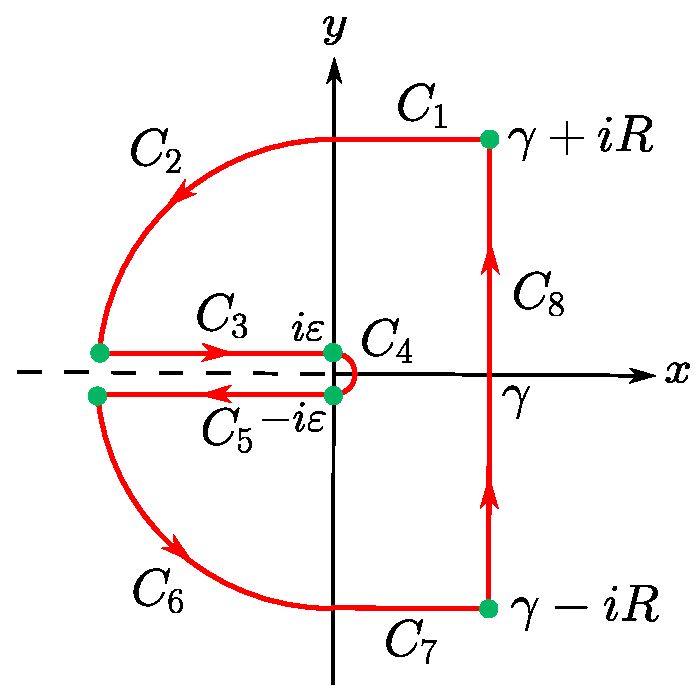
\includegraphics[scale = 0.6]{Figuras/InversaLaplace2.pdf}
%         \caption{Contorno de integración para la transformada inversa de Laplace $1/\sqrt{s}$.}
%         \label{fig:InvLaplaceBranchCut}
%     \end{figure}

%     Como el integrando es analítico en el interior del contorno cerrado, por el teorema de Cauchy-Goursat,
%     $$\sum_{k=1}^{8} \int_{C_k} e^{st} \frac{1}{\sqrt{s}} \,ds = 0.$$

%     Mostremos que la integral en torno a $C_1: s = x + i R, 0\leq x \leq \gamma$, se desvanece cuando $R \to \infty$. 

%     Para $s \in C_1$, tenemos que
%     $$\left|e^{st} \frac{1}{\sqrt{s}} \right| = \frac{e^{\real(s) t}}{\sqrt{|s|}} \leq \frac{e^{\gamma t}}{\sqrt{R}}.$$

%     Luego,
%     $$\left|\int_{C_1} e^{st} \frac{1}{\sqrt{s}} \,ds \right| \leq \int_0^{\gamma} \frac{e^{\gamma t}}{\sqrt{R}} \,dx = \frac{\gamma e^{\gamma t}}{\sqrt{R}} \overset{R \to \infty}{\longrightarrow} 0.$$

%     Similarmente, se prueba que la integral en torno a $C_7: s = x - i R, 0 \leq x \leq \gamma$, se desvanece cuando $R \to \infty$.

%     Ahora, mostremos que la integral en torno a $C_2: s = Re^{i\theta}, \pi/2 \leq \theta < \pi$, se desvanece cuando $R \to \infty$. 

%      Para $s \in C_2$, tenemos que
%     $$\left|e^{st} \frac{1}{\sqrt{s}} \right| = \frac{e^{\real(s) t}}{\sqrt{|s|}} = e^{R t \cos \theta }\frac{1}{\sqrt{R}}.$$

%     Luego,
%     $$\left|\int_{C_2} e^{st} \frac{1}{\sqrt{s}} \,ds \right| \leq \frac{1}{\sqrt{R}} \int_{\pi/2}^{\pi} e^{Rt \cos \theta} d\theta.$$

%     Haciendo la sustitución $\phi = \theta - (\pi/2) \Rightarrow d\phi = d\theta$, en la integral y usando la desigualdad de Jordan, obtenemos
%     $$\left|\int_{C_2} e^{st} \frac{1}{\sqrt{s}} \,ds \right| \leq \frac{1}{\sqrt{R}} \int_{0}^{\pi/2} e^{-Rt \sin \phi} d\phi \leq \frac{1}{\sqrt{R}} \frac{\pi}{2 R t}\overset{R \to \infty}{\longrightarrow} 0.$$

%     Similarmente, se prueba que la integral en torno a $C_6$ se desvanece.

%     Podemos mostrar que la integral en torno a $C_4: s = \varepsilon e^{i\theta}, -\pi/2 \leq \theta \leq \pi/2$, se desvanece cuando $\varepsilon \to 0$.

%     Para $s \in C_4$, tenemos que
%     $$\left|e^{st} \frac{1}{\sqrt{s}} \right| = \frac{e^{\real(s) t}}{\sqrt{|s|}} = \frac{e^{\varepsilon t \cos\theta}}{\sqrt{\varepsilon}} \leq  \frac{e^{\varepsilon t}}{\sqrt{\varepsilon}}.$$

%     Luego,
%     $$\left|\int_{C_4} e^{st} \frac{1}{\sqrt{s}} \,ds \right| \leq \frac{e^{\varepsilon t}}{\sqrt{\varepsilon}} \int_{-\pi/2}^{ \pi/2} \varepsilon d\theta = \frac{e^{\varepsilon t}}{\sqrt{\varepsilon}} (\pi \varepsilon) \overset{\varepsilon \to 0}{\longrightarrow} 0.$$

%     Entonces,
%     $$\int_{C_3} e^{st} \frac{1}{\sqrt{s}} \,ds + \int_{C_5} e^{st} \frac{1}{\sqrt{s}} \,ds + \int_{C_8} e^{st} \frac{1}{\sqrt{s}} \,ds = 0.$$

%     Tomando el límite $R \to \infty$ y $\varepsilon \to 0$, podemos expresar la transformada inversa de Laplace como
%     $$\mathcal{L}^{-1}\left\{ \frac{1}{\sqrt{s}}\right\} = \frac{1}{2\pi i} \int_{\gamma - i\infty}^{\gamma + i \infty} e^{st} \frac{1}{\sqrt{s}} \,ds = - \frac{1}{2\pi i} \lim_{R\to\infty}  \lim_{\varepsilon \to 0} \left[ \int_{C_3} e^{st} \frac{1}{\sqrt{s}} \,ds +  \int_{C_5} e^{st} \frac{1}{\sqrt{s}} \,ds\right].$$

%     Bajo estos límites, tenemos que en $C_3$, $s = x$, $ds = dx$, con $x$ desde $-\infty$ a $0$, y en $C_5$, $s = x$, $ds = dx$, con $x$ desde $0$ a $-\infty$.  Luego,
%     \begin{align*}
%        \mathcal{L}^{-1}\left\{ \frac{1}{\sqrt{s}}\right\} &= - \frac{1}{2\pi i} \int_{-\infty}^0 e^{xt} \frac{e^{-i\pi/2}}{\sqrt{-x}} \,dx - \frac{1}{2\pi i} \int_0^{-\infty} e^{xt} \frac{e^{i\pi/2}}{\sqrt{-x}} \,dx \\
%        &= -\frac{1}{2\pi} \int_{\infty}^0 e^{-xt} \frac{1}{\sqrt{x}} \,dx + \frac{1}{2\pi} \int_0^{\infty} e^{-xt} \frac{1}{\sqrt{x}} \,dx \\
%        &= \frac{1}{\pi} \int_0^{\infty} e^{-xt} \frac{1}{\sqrt{x}} \,dx.
%     \end{align*}

%     Haciendo la sustitución $u = xt \Rightarrow du = t dx$,
%     $$ \mathcal{L}^{-1}\left\{ \frac{1}{\sqrt{s}}\right\}  = \frac{1}{\pi \sqrt{t}} \int_0^{\infty} e^{-u} \frac{1}{\sqrt{u}} \,du.$$

%     Pero,
%     $$\int_0^{\infty} e^{-u} \frac{1}{\sqrt{u}} \,du = \Gamma\left( \frac{1}{2}\right) = \sqrt{\pi}.$$

%     Por lo tanto,
%     $$ \mathcal{L}^{-1}\left\{ \frac{1}{\sqrt{s}}\right\} = \frac{1}{\sqrt{\pi t}}, \quad t > 0.$$
% \end{ejemplo}

\subsection{Propiedades de la transformada de Laplace}    

\begin{teorema}
    Si $f$ y $g$ son funciones cuyas transformadas de Laplace existen para $\real(s) > \alpha$ y sean $a, b \in \mathbb{R}$. Entonces, 
\begin{enumerate}
    \item \textbf{Linealidad:} Para $\real(s) > \alpha$,
    $$\mathcal{L}\{a f(t) + b g(t)\} = a \mathcal{L}\{f(t)\} + b \mathcal{L}\{g(t)\}.$$ 

    \item \textbf{Escalonamiento:} Para $\real(s) > \alpha \cdot \beta$,
    $$\mathcal{L}\{f(\beta t) \} = \frac{1}{\beta} F \left( \frac{s}{\beta}\right), \quad \beta > 0.$$ 
    
    \item \textbf{Desplazamiento en el plano $s$:} Para $\real(s) > \alpha + a$,
    $$\mathcal{L}\{e^{at} f(t)\} = F(s-a).$$
\end{enumerate}
\end{teorema}

\begin{ejemplo}
    Determine la transformada de Laplace de $e^{at} \sin(bt)$.

    \textbf{Solución:} En la primera sección, vimos que
    $$\mathcal{L}\{\sin(bt)\} = F(s) = \frac{b}{s^2+b^2}, \quad \real(s) > 0.$$

    Luego, por la propiedad de desplazamiento,
    $$\mathcal{L}\{e^{at} \sin(bt)\} = F(s-a) = \frac{b}{(s-a)^2+b^2}, \quad \real(s) > a.$$
\end{ejemplo}

\begin{teorema}[Propiedad de la derivada]
    Sea $f$ continua en $]0, + \infty [$ y $f'(t)$ continua por tramos en $[0, + \infty[$, ambas de orden exponencial $\alpha$. Entonces, para $\real(s) > \alpha$,
    $$\mathcal{L}\{f'(t)\} = s \mathcal{L}\{f(t)\} - f(0^+),$$

    donde $f(0^+) = \lim\limits_{t \to 0^+} f(t)$. 
\end{teorema}

En general, la transformada de Laplace de derivadas de orden superior están dadas por el siguiente teorema.

\begin{teorema}[Transformada de Laplace de derivadas de orden superior]
 Sean $f, f', \dots, f^{(n-1)}$ continuas para todo $t>0$ y sea $f^{(n)}$ continua por tramos en $[0,+\infty[$, con todas estas funciones de orden exponencial $\alpha$. Entonces, para $\real(s) > \alpha$,
$$\mathcal{L}\{f^{(n)}(t)\} = s^n \mathcal{L}\{f(t)\} - s^{n-1} f(0^+) - s^{n-2} f'(0^+) - \cdots - f^{(n-1)}(0^+). \label{LaplaceDerivada}$$

\end{teorema}

\begin{ejemplo}
Calcule 
$$\mathcal{L}\left\{\sin^2(at)\right\}.$$   

\textbf{Solución:} Sea $f(t) = \sin^2(at)$, entonces
$$f'(t) = 2a \sin(at) \cos(at) = a \sin(2at).$$

Como $f(0) = 0$ y $\frac{2a^2}{s^2+4a^2} = \mathcal{L}\{f'(t)\} = s \mathcal{L}\{f(t)\} - f(0)$, obtenemos
$$\mathcal{L}\left\{\sin^2(at)\right\} = \frac{2a^2}{s(s^2+4a^2)}, \quad \real(s) > 0.$$
\end{ejemplo}

Hemos determinando la transformada de Laplace de la derivada de una función $f$, es natural preguntarse sobre la transformada de una función definida por una integral:
$$g(t) = \int_0^t f(t') \,dt'.$$

\begin{teorema}
     Sea la función $f(t)$ continua por tramos y de orden exponencial $\alpha$. Entonces,
     $$\mathcal{L} \left\{ \int_0^t f(t') \,dt'\right\} = \frac{1}{s} \mathcal{L}\{f(t)\}, \quad \real(s) > \alpha.$$
\end{teorema}

\begin{demo}
Caso particular del teorema \ref{Teo:Convolucion} para 
$$(f * g)(t) = \int_0^t f(u) g(t-u) \,du,$$

con $g(t) = 1$.
\end{demo}

Para funciones periódicas, tenemos el siguiente teorema.

\begin{teorema}
 Sea $f$ una función continua por tramos en el intervalo $[0,T]$ y periódica con periodo $T>0$. Entonces $f$ tiene transformada de Laplace dada por
\begin{equation*}
\mathcal{L}\{f(t)\} = \frac{\int_0^T e^{-st} f(t) dt}{1-e^{-Ts}}, \quad \real(s) > 0.
\end{equation*}
   
\end{teorema}

\begin{ejemplo}
    Encuentre la transformada de Laplace de
    $$f(t) = \left\{ \begin{array}{cl}
     1,& \text{si} ~ 0 \leq t < \pi  \\
     0,& \text{si} ~ \pi \leq t < 2\pi
    \end{array} \right.$$

    y $f(t+ 2\pi) = f(t)$ para $t > 0$, ésto es, $f(t)$ es periódica para $t > 0$.

    \textbf{Solución:} Como $f$ es periódica de periodo $T = 2\pi$, tenemos que
    \begin{align*}
        \mathcal{L}\{f(t)\} &= \frac{\int_0^{2\pi} e^{-st} f(t) \,dt}{1-e^{-2\pi s}} \\
        &= \frac{\int_0^{\pi} e^{-st}\,dt}{1-e^{-2\pi s}} \\
        &= \frac{1-e^{-\pi s}}{s(1-e^{-2\pi s})} \\
        &= \frac{1}{s(1+e^{-\pi s})}.
    \end{align*}
\end{ejemplo}

\begin{teorema}[Integral de una transformada]
   Si $\int_0^{\beta} \frac{f(t)}{t} \,dt$ existe para $\beta > 0$ y $f(t)$ es de orden exponencial $\alpha$, entonces
   $$\mathcal{L}\left\{\frac{f(t)}{t}\right\} = \int_s^{\infty} F(u) \,du, \quad s > \alpha.$$
\end{teorema}

\subsection{Convolución}

\begin{defi}
   Sean $f$ y $g$ funciones continuas por tramos en $[0, \infty[$. La \textbf{convolución} de $f$ y $g$, que se denota $f*g$, se define como
\begin{equation*}
(f*g)(t) := \int_0^t f(t-u)g(u) \, du.
\end{equation*}  
\end{defi}

Es claro que la convolución es distinta de la multiplicación común. Por ejemplo, $1*1 = t \neq 1$, y en general, $1*f \neq f$. Sin embargo, la convolución sí satisface algunas propiedades de la multiplicación.

\begin{teorema}[Propiedades de la convolución]
Sean $f$, $g$ y $h$ continuas por tramos en $[0,  \infty[$. Entonces,

\begin{itemize}
\item[(i)] $f*g = g*f$,

\item[(ii)] $f*(g*h) = (f*g)*h$,  

\item[(iii)] $f*(g+h) = f*g + f*h$. 
\end{itemize} 
\end{teorema}

Al igual que para la transformada de Fourier, la transformada de Laplace de la convolución obedece el siguiente teorema.

\begin{teorema}[de Convolución] \label{Teo:Convolucion}
    Sean $f$ y $g$ funciones continuas por tramos, de orden exponencial, tales que:
    \begin{equation*}
    \mathcal{L}\{f(t)\} = F(s) ~~\mbox{y}~~ \mathcal{L}\{g(t)\} = G(s),
    \end{equation*}

    entonces
    \begin{equation*}
    \mathcal{L}\{(f*g)(t)\} = F(s)G(s),
    \end{equation*}

    o, de manera equivalente,
    \begin{equation*}
    \mathcal{L}^{-1}\{F(s)G(s)\}(t) = (f*g)(t).
    \end{equation*}    
\end{teorema}

\begin{demo}

Tomando la transformada de Laplace de la convolución $f * g$,
$$\mathcal{L}\{(f*g)(t)\} = \int_0^{\infty} e^{-st} \int_0^t f(t-u) g(u) \,du \,dt = \int_0^{\infty} \int_0^t e^{-st}  f(t-u) g(u) \,du \,dt.$$

La región de integración se ilustra en la figura \ref{fig:Convolucion2}.

\begin{figure}[H]
    \centering
    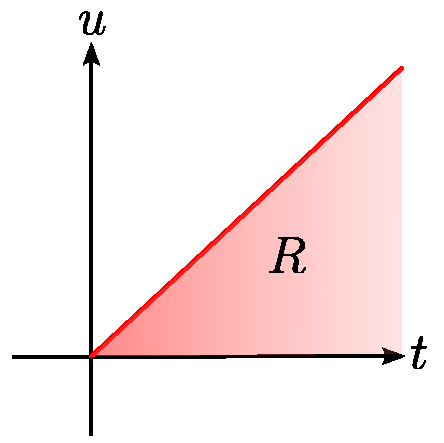
\includegraphics[scale = 0.6]{Figuras/Laplace-Convolucion-2.pdf}
    \caption{Región de integración.}
    \label{fig:Convolucion2}
\end{figure}

Luego, haciendo un cambio en el orden de integración, se tiene
$$\mathcal{L}\{(f*g)(t)\} = \int_0^{\infty} \int_u^{\infty} e^{-st} f(t-u) g(u) \,dt\,du.$$

Si hacemos el cambio de variable $v = t-u$ en la integral interior, obtenemos que
\begin{align*}
    \mathcal{L}\{(f*g)(t)\} &= \int_0^{\infty} g(u) \int_0^{\infty} e^{-s(u+v)} f(v) \,dv \,du \\
    &= \left(\int_0^{\infty} g(u) e^{-su} du \right)\left(\int_0^{\infty} f(v) e^{-sv} \,dv  \right) \\
    &= F(s)G(s). 
\end{align*}

\end{demo}

\begin{ejemplo}
Calcule
$$\mathcal{L}^{-1} \left\{ \frac{s}{(s^2+1)^2} \right\}.$$

\textbf{Solución:} Notemos que 
\begin{equation*}
\mathcal{L}^{-1} \left\{ \frac{s}{(s^2+1)^2} \right\} = \mathcal{L}^{-1} \left\{ \frac{s}{s^2+1} \cdot \frac{1}{s^2+1} \right\}.
\end{equation*}

Como
\begin{equation*}
\mathcal{L}\{\cos(t)\} = \frac{s}{s^2+1} ~~\mbox{y}~~ \mathcal{L}\{\sin(t)\} = \frac{1}{s^2+1},
\end{equation*}

tenemos, por el teorema de convolución, que
\begin{align*}
    \mathcal{L}^{-1} \left\{ \frac{s}{(s^2+1)^2} \right\} &=\cos(t) *\sin(t)  \\
    &= \int_0^t \sin(t-u) \cos(u) \,du \\
    &= \int_0^t (\sin(t) \cos(u) - \cos(u) \sin(u)) \cos(u) \,du  \\
    &= \sin(t) \int_0^t \cos^2(u) \,du - \cos(t) \int_0^t \sin (u) \cos(u) \,du \\
    &= \sin(t) \left[ \frac{1}{2} u + \frac{\sin(2u)}{4} \right]_0^t - \cos(t) \left[ \frac{\sin^2(u)}{2} \right]_0^t \\
    &= \frac{t \sin(t)}{2} + \frac{\sin(2t)}{4} \sin(t) - \cos(t) \frac{\sin^2(t)}{2} \\
    &= \frac{t \sin(t) }{2}.
\end{align*}

Por lo tanto,
$$\mathcal{L}^{-1} \left\{ \frac{s}{(s^2+1)^2} \right\} = \frac{t \sin(t) }{2}.$$   
\end{ejemplo}

\subsection{Aplicaciones de la transformada de Laplace}

La transformada de Laplace, al igual que la transformada de Fourier, nos permite convertir ecuaciones diferenciales en ecuaciones algebraicas, con una diferencia: se requiere el valor de la función en un punto dado. Lo anterior nos entrega una ligera ventaja y es que una vez que se invierta la transformada, tendremos de inmediato la solución al problema, recalcando que el dominio de validez de la función encontrada es para $t > 0$. Otra diferencia relevante es que, mientras la transformada de Fourier sólo se puede aplicar a funciones que decrecen rápidamente a cero, la transformada de Laplace está bien definida incluso para funciones de crecimiento exponencial. Entonces, si estamos en presencia de un sistema físico caracterizado por una variable que crece exponencialmente, es bastante probable que la transformada de Fourier dé resultados sin sentido físico.

A continuación expondremos dos situaciones en las cuales el uso de la transformada de Laplace es ventajoso.

\subsubsection{Ecuaciones diferenciales lineales con coeficientes constantes}

\begin{ejemplo}
    Consideremos la ecuación diferencial
    $$y'(t) + y(t) = \cos(t), \quad \text{para} ~ t > 0, \quad y(0) = 1.$$

    Apliquemos la transformada de Laplace a ambos lados de la ecuación:
    $$\mathcal{L}\{y'(t)\} - \mathcal{L}\{y(t)\} = \mathcal{L}\{\cos(t)\}.$$

    Evaluamos la transformada de la primera derivada, usando los teoremas enunciados durante el capítulo.
    $$\mathcal{L}\{y'(t)\} = s Y(s) - y(0) = s Y(s) - 1,$$

    donde $Y(s) = \mathcal{L}\{y(t)\}$. Luego, la ecuación diferencial nos queda:
    \begin{align*}
        sY(s) - 1 + Y(s) &= \frac{s}{s^2+1} \\
        \Rightarrow \quad Y(s) &= \frac{s}{(s+1)(s^2+1)} + \frac{1}{s+1} \\
        \Rightarrow \quad Y(s) &= \frac{1/2}{s+1} + \frac{1}{2} \frac{s+1}{s^2+1}.
    \end{align*}

    Aplicando la transformada de Laplace inversa,
    $$y(t) = \frac{1}{2} e^{-t} + \frac{1}{2} \cos(t) + \frac{1}{2} \sin(t), \quad t > 0.$$
\end{ejemplo}

% \subsubsection{Ecuaciones integrales}

% Una \textbf{ecuación integral} es aquella ecuación donde la función incógnita $\varphi(x)$ se encuentra dentro de una integral. Estas ecuaciones integrales se clasifican en dos formas \cite{Arfken}:
% \begin{itemize}
%     \item Si los límites de integración están fijos, llamamos la ecuación una \textbf{ecuación de Fredholm}; si un límite es variable, es una \textbf{ecuación de Volterra}.

%     \item Si la función incógnita aparece solo en la integral, la etiquetamos como de \textbf{primera especie}. Si aparece tanto dentro como fuera de la integral, la etiquetemos como de \textbf{segunda especie}.
% \end{itemize}

% A continuación algunos ejemplos de estas definiciones donde $\varphi(t)$ es la función desconocida, $K(x,t)$ una función de dos variables que la llamaremos \textbf{kernel}, y $f(x)$ una función que asumimos conocida.

% \begin{enumerate}
%     \item \textbf{Ecuación de Fredholm de primera especie}:
%     $$f(x) = \int_a^b K(x,t) \varphi(t) \,dt.$$

%     \item \textbf{Ecuación de Fredholm de segunda especie}:
%     $$\varphi(x) = f(x) + \lambda \int_a^b K(x,t) \varphi(t) \,dt.$$

%     \item \textbf{Ecuación de Volterra de primera especie}:
%     $$f(x) = \int_a^x K(x,t) \varphi(t) \,dt.$$

%     \item \textbf{Ecuación de Volterra de segunda especie}:
%     $$\varphi(x) = f(x) + \int_a^x K(x,t) \varphi(t) \,dt.$$
% \end{enumerate}

% En esta sección nos enfocaremos en ecuaciones de Volterra para $K(x,t) = K(x-t)$, de tal forma que
% $$\int_a^x K(x,t) \varphi(t) \,dt = (K * \varphi)(x).$$

% Para ilustrar el método, consideremos la situación física planteada en el siguiente ejemplo.

% \begin{ejemplo}[Problema de la tautócrona]
%     Una partícula de masa $m$ resbala (parte del reposo), sin roce, sobre una curva bajo el efecto de la gravedad. Buscamos determinar la forma de la curva de modo que el tiempo que le toma a la partícula en llegar al suelo sea independiente del punto de lanzamiento. 

%     \begin{figure}[H]
%         \centering
%         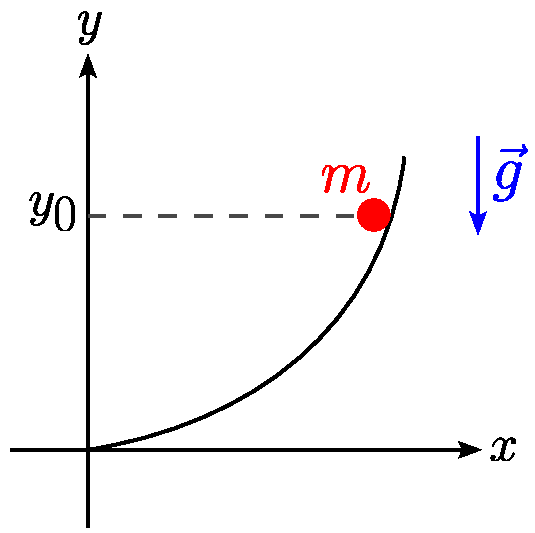
\includegraphics[scale = 0.65]{Figuras/tautocrona.pdf}
%         \caption{Esquema de la situación física.}
%         \label{fig:tautocrona}
%     \end{figure}

%     Como estamos en presencia de fuerzas conservativas, la  energía se conserva durante todo el trayecto para todo $y$, ésto es,
%     \begin{alignat*}{3}
%     &               &\quad   \text{Energía inicial en $y_0$} &= \text{Energía final en $y$} \\
%     &  \Rightarrow  &\quad      mgy_0 &= \frac{1}{2} mv^2 + mgy \\
%     &  \Rightarrow  &\quad   \frac{1}{2} mv^2 &= mg(y_0 - y) \\
%     &  \Rightarrow  &\quad   v &= \sqrt{2 g} \sqrt{y_0-y}, 
%     \end{alignat*}   
    
%     donde $y_0$ es la altura inicial. El tiempo de descenso está dado por
%     $$T(y_0) = \int \frac{ds}{v} = \int_{y_0}^0 \frac{1}{v} \frac{ds}{dy} dy = - \int_0^{y_0} f(y) (y_0 - y)^{-1/2} \frac{1}{\sqrt{2g}} dy,$$

%     donde $f(y) = ds/dy$. Ahora, si suponemos que $T(y_0)$ es constante $T_0$, ésto es, independiente del punto de partida $y_0$. La condición queda
%     $$\int_0^{y_0} f(y) (y_0 - y)^{-1/2} \,dy = C_0,$$

%     donde $C_0 = -\sqrt{2g} T_0$. Aplicando la transformada de Laplace  a ambos lados de la ecuación:
%     $$\mathcal{L}\left\{\int_0^{y_0} f(y) (y_0 - y)^{-1/2} \,dy \right\} = \mathcal{L}\{C_0\} = \frac{C_0}{s}.$$
    
%     Por el teorema de convolución, tenemos que
%     $$\mathcal{L}\{f(y)\} \mathcal{L}\{y^{-1/2}\} = \frac{C_0}{s} \Rightarrow \mathcal{L}\{f(y)\} = \frac{C_0/s}{\mathcal{L}\{y^{-1/2}\}}.$$

%     Pero,
%     $$\mathcal{L}\{y^{-1/2}\} = \int_0^{\infty} e^{-sy} \frac{1}{\sqrt{y}} \,dy \overset{\textcolor{blue}{t = sy}}{=} \frac{1}{\sqrt{s}}\int_0^{\infty} e^{-t} \frac{1}{\sqrt{t}} \,dt = \frac{\Gamma\left(\frac{1}{2}\right)}{\sqrt{s}}.$$

%     Así,
%     $$\mathcal{L}\{f(y)\} = \frac{C_0}{s} \frac{\sqrt{s}}{\Gamma\left(\frac{1}{2}\right)} = \frac{C_0}{\sqrt{\pi}} \frac{1}{\sqrt{s}}.$$

%     Tomando la transformada inversando y usando el resultado del ejemplo \ref{Inv_Laplace_ej_branch}, obtenemos 
%     $$f(y) = \frac{C_0}{\pi} \frac{1}{\sqrt{y}} = \frac{C}{\sqrt{y}},$$

%     donde $C = C_0/\pi$. Recordando que $f(y) = ds/dy$, notemos que
%     \begin{align*}
%         ds^2 = dx^2 + dy^2 &\Rightarrow dx = \sqrt{ds^2 - dy^2} \\
%         &\Rightarrow dx = \sqrt{\left( \frac{ds}{dy} dy\right)^2 - dy^2} \\
%         &\Rightarrow dx = \sqrt{\left(\frac{ds}{dy}\right)^2 - 1} \,dy \\
%         &\Rightarrow \frac{dx}{dy} = \sqrt{\frac{C^2}{y} - 1}. 
%     \end{align*}

%     Integrando con respecto a $y$,
%     $$x(y) = \int \sqrt{\frac{C^2}{y} - 1} \,dy.$$

%     Haciendo el cambio de variable $y = C^2 \sin^2 (\phi) \Rightarrow dy = 2 C^2 \sin(\phi) \cos(\phi) \,d\phi$,
%     \begin{align*}
%         x &= \int \sqrt{\csc^2(\phi) - 1} \, 2 C^2 \sin(\phi) \cos(\phi) \,d\phi \\
%         &= 2C^2 \int \sqrt{\cot^2(\phi)}  \sin(\phi) \cos(\phi) \,d\phi \\
%         &= 2C^2 \int \cos^2(\phi) \,d\phi \\
%         &=  \frac{C^2}{2} (2\phi + \sin(2\phi)) + D,
%     \end{align*}

%     donde $D$ es una constante de integración. Entonces,
%     \begin{align*}
%         x &= \frac{C^2}{2} (2\phi + \sin(2\phi)) + D, \\
%         y &= \frac{C^2}{2} (1 - \cos(2\phi)).
%     \end{align*}

%     La curva debe pasar por el origen $(0,0)$, así que $D = 0$, y si definimos un nuevo parámetro $\theta = 2\phi$, encontramos que
%     \begin{align*}
%         x &= \frac{C^2}{2} (\theta + \sin(\theta)), \\
%         y &= \frac{C^2}{2} (1 - \cos(\theta)).
%     \end{align*}

%     Estas son las ecuaciones paramétricas de un cicloide.
% \end{ejemplo}

\subsubsection{Sistema de ecuaciones lineales}

La transformada de Laplace puede ser usada para convertir un sistema de ecuaciones diferenciales con coeficientes constantes en un sistema de ecuaciones algebraicas. 

\begin{ejemplo}
    Consideremos el circuito de la figura \ref{fig:Circuit}. 
    
    \begin{figure}[H]
        \centering
        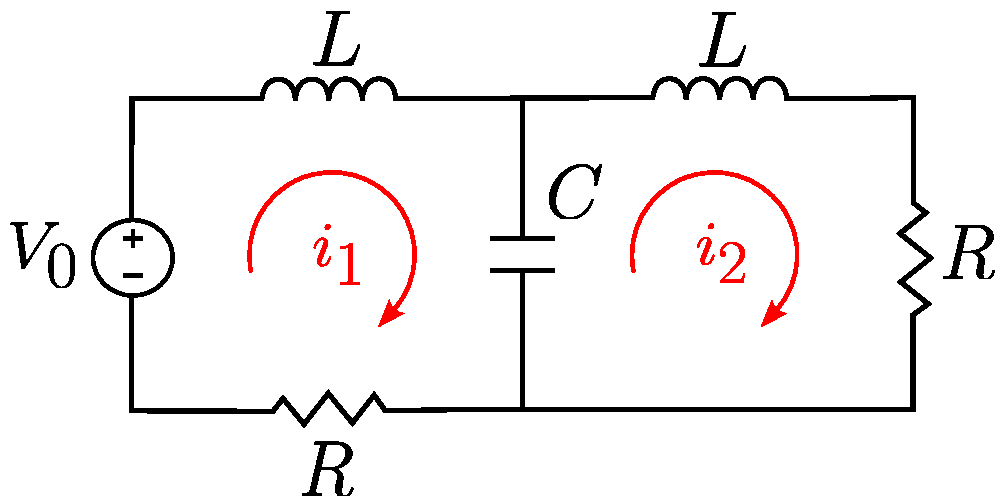
\includegraphics[scale = 0.65]{Figuras/Circuito.pdf}
        \caption{Circuito eléctrico.}
        \label{fig:Circuit}
    \end{figure}
    
    Usando las leyes de Kirchhoff, encontramos el siguiente sistema de ecuaciones diferenciales.
    \begin{align*}
        L \frac{di_1}{dt} + Ri_1 + \frac{q}{C} &= V_0, \\
        L \frac{di_2}{dt} + Ri_2 - \frac{q}{C} &= 0, \\
        \frac{dq}{dt} &= i_1 - i_2.
    \end{align*}
    
    Inicialmente el capacitador se encuentra descargado y las corrientes inducidas por las inductancias son despreciables de tal forma que se tienen las condiciones iniciales:
    $$i_1(0) = i_2(0) = \frac{V_0}{2R}, \quad q(0) = 0.$$

    Aplicamos la transformada de Laplace al sistema de ecuaciones diferenciales.
    \begin{align*}
        L\left( sI_1(s) - \frac{V_0}{2R} \right) + RI_1(s) + \frac{Q(s)}{C} &= \frac{V_0}{s}, \\
       L\left( sI_2(s) - \frac{V_0}{2R} \right) + RI_2(s) - \frac{Q(s)}{C}  &= 0, \\
        sQ(s) &= I_1(s) - I_2(s),
    \end{align*}

    donde $I_1(s) = \mathcal{L}\{i_1(t)\}$, $I_2(s) = \mathcal{L}\{i_2(t)\}$ y $Q(s) = \mathcal{L}\{q(t)\}$. Despejando estas cantidades:
    \begin{align*}
        I_1 &= \frac{V_0}{2} \left(\frac{1}{Rs} + \frac{1/L}{s^2 + R s/L + 2/(CL)} \right) \\
        I_2 &= \frac{V_0}{2} \left(\frac{1}{Rs} - \frac{1/L}{s^2 + R s/L + 2/(CL)} \right) \\
            Q &= \frac{C V_0}{2} \left( \frac{1}{s} - \frac{s+R/L}{s^2 + Rs/L + 2/(CL)} \right)
    \end{align*}

    Factorizando las polinomios de los denominadores.
    \begin{align*}
        I_1 &= \frac{V_0}{2} \left(\frac{1}{Rs} + \frac{1/L}{(s+\alpha - i \omega)(s + \alpha + i \omega)} \right) \\
        I_2 &= \frac{V_0}{2} \left(\frac{1}{Rs} - \frac{1/L}{(s+\alpha - i\omega)(s+\alpha + i \omega)} \right) \\
        Q &= \frac{C V_0}{2} \left( \frac{1}{s} - \frac{s+2\alpha}{(s+\alpha - i\omega)(s+\alpha + i \omega))} \right).
    \end{align*}

    Aquí hemos definido
    $$\alpha = \frac{R}{2L} \quad \text{y} \quad \omega^2 = \frac{2}{LC} - \alpha^2.$$

    Expandiendo las funciones en fracciones parciales.
    \begin{align*}
        I_1 &= \frac{V_0}{2} \left(\frac{1}{Rs} + \frac{i}{2\omega L} \left(\frac{1}{s+\alpha + i\omega} - \frac{1}{s+\alpha - i\omega} \right) \right) \\
        I_2 &= \frac{V_0}{2} \left(\frac{1}{Rs} - \frac{i}{2\omega L} \left(\frac{1}{s+\alpha + i\omega} - \frac{1}{s+\alpha - i\omega} \right) \right) \\
        Q &= \frac{C V_0}{2} \left( \frac{1}{s} + \frac{i}{2\omega} \left( \frac{\alpha + i\omega}{s+\alpha - i\omega} - \frac{\alpha - i \omega}{s+\alpha +i\Omega} \right) \right).
    \end{align*}

    Ahora, aplicamos la transformada inversa, teniendo en consideración que
    $$\mathcal{L}^{-1}\left\{ \frac{1}{s-a} \right\} = e^{at},$$
     \begin{align*}
        i_1 &= \frac{V_0}{2} \left(\frac{1}{R} + \frac{i}{2\omega L} \left( e^{(-\alpha - i\omega)t} - e^{(-\alpha + i\omega)t}\right) \right) \\
        i_2 &= \frac{V_0}{2} \left(\frac{1}{R} - \frac{i}{2\omega L} \left( e^{(-\alpha - i\omega)t} - e^{(-\alpha + i \omega)t}\right) \right) \\
        q &= \frac{C V_0}{2} \left( 1 + \frac{i}{2\omega} \left( (\alpha + i\omega) e^{(-\alpha + i \omega)t} - (\alpha - i\omega)e^{(-\alpha - i\omega)t} \right) \right).
    \end{align*}

    Simplicando las expresiones, obtenemos las soluciones.
    \begin{align*}
        i_1 &= \frac{V_0}{2} \left(\frac{1}{R} + \frac{1}{\omega L} e^{-\alpha t}\sin(\omega t) \right), \\
        i_2 &= \frac{V_0}{2} \left(\frac{1}{R} - \frac{1}{\omega L} e^{-\alpha t}\sin(\omega t) \right), \\
        q &= \frac{CV_0}{2} \left( 1- e^{-\alpha t} \left( \cos(\omega t) + \frac{\alpha}{\omega} \sin(\omega t) \right)\right).
    \end{align*}
\end{ejemplo}








 

\chapter{Funciones de Legendre}

Como vimos anteriormente en el capítulo \ref{chap:MSV}, al resolver la ecuación de Helmholtz en coordenadas esféricas, podemos obtener dos ecucaciones, según el valor de la constante de separación $m^2$. 

\section{Ecuación y Funciones de Legendre}

Analizaremos en primer lugar el caso en que $m=0$, donde luego del cambio de variables $x = \cos \theta$, obtuvimos la EDO
% \begin{equation}
%     \frac{1}{\sin\theta} \frac{d}{d\theta}\left( \sin\theta \frac{d\Theta}{d\theta} \right) + \lambda \Theta = 0 \ ,
% \end{equation}
% que al considerar el cambio de variables $x = \cos\theta$, y llamar a $\Theta(\theta) = \Theta(\arccos(x)) = y(x)$, de modo que
% \begin{equation}
%     \frac{d}{d\theta} = \frac{dx}{d\theta} \frac{d}{dx} = -\sin\theta \frac{d}{dx} \ ,
% \end{equation}
% con lo que podremos escribir la ecuación como
\begin{equation}
    % \frac{1}{\sin\theta}(-\sin\theta)\frac{d}{dx}\left( \sin\theta (-\sin\theta) \frac{dy}{dx} \right) + \lambda y = 
    \frac{d}{dx}\left( (1-x^2) \frac{dy}{dx} \right) + \lambda y = 0 \ ,
\end{equation}
expresión que nombraremos como \textbf{ecuación de Legendre}, y que también puede ser escrita de forma más explícita como
\begin{equation}\label{eq:legendre_explicit}
    (1-x^2)\frac{d^2y}{dx^2} - 2x \frac{dy}{dx} + \lambda y = 0 \ .
\end{equation}

% Observamos que hemos escrito la ecuación de Legendre en la forma de una ecuación de Sturm-Liouville, con $p(x) = 1-x^2$ y $q(x) = r(x) = 1$. Observamos que,
Dado que $x=\cos\theta$, nuestra ecuación, y por ello sus soluciones, están definidas en el intervalo $[-1,1]$. Nos interesa que estos casos extremos posean soluciones finitas, lo que nos permitirá encontrar el valor de $\lambda$ para esta ecuación.

\subsection{Resolviendo la ecuación de Legendre}

% En primer lugar, escribimos la ecuación de forma más explícita, es decir,
% \begin{equation}\label{eq:legendre_explicit}
%     (1-x^2)y''(x) - 2x y'(x) + \lambda y(x) = 0 \ .
% \end{equation}

Utilizando el método de series, observamos que $P(x) = -2x/(1-x^2)$, y que $Q(x) = \lambda/(1-x^2)$. Ambas expresiones tienen puntos singulares en $x = \pm 1$, pero $x=0$ es un punto ordinario. Por ello, planteamos soluciones de la forma
\begin{equation}
    % \begin{dcases}
        y(x) = \sum_{k=0}^{\infty} a_k x^k \ ,
        %  \\
    %     y'(x) & = \sum_{k=1}^{\infty} k a_k x^{k-1} \\
    %     y''(x) & = \sum_{k=2}^{\infty} (k-1)k a_k x^{k-2} \\
    %     & = \sum_{k=0}^{\infty} (k+1) (k+2) a_{k-2} x^k 
    % \end{dcases} \ ,
\end{equation}
de modo que sustituyendo en la expresión \eqref{eq:legendre_explicit} tenemos 
\begin{align*}
    \sum_{k=0}^{\infty} (k+1)(k+2) a_{k+2} x^k - \sum_{k=0}^{\infty} (k-1) k a_k x^k - 2 \sum_{k=1}^{\infty} k a_k x^k + \lambda \sum_{k=0}^{\infty} a_k x^k & = 0 \ , \\
    \sum_{k=0}^{\infty} \left[ (k+1)(k+2) a_{k+2} - k(k-1)a_k  - 2k a_k + \lambda a_k \right]x^k & = 0 \ ,
\end{align*}
donde hemos usado que $\sum_{k=0}^{\infty} k = 0 + \sum_{k=1}^{\infty} k$. Dado que $x^k = 0$ corresponde a la solución trivial, analizamos la relación entre los coeficientes de nuestra ecuación,
\begin{equation}
    (k+1)(k+2) a_{k+2} - [(k-1) k + 2k - \lambda]a_k = 0 \ ,
\end{equation}
de donde encontramos la siguiente relación de recurrencia,
\begin{equation}\label{eq:recurrencia_legendre}
    a_{k+2} = \frac{k(k+1) - \lambda}{(k+1)(k+2)}a_k \ ,
\end{equation}
de modo que dados unos valores para $a_0$ y $a_1$ podremos determinar todos los coeficientes de nuestra expresión. Luego, si desarrollamos los términos pares e impares por separado, podemos observar la siguiente recurrencia,
\begin{align*}
    a_2 & = \frac{-\lambda}{2} a_0 \\
    a_4 & = \frac{2(2+1) - \lambda}{3 \cdot 4} a_2 = \frac{-\lambda(2(2+1)-\lambda)}{4!}a_0 \\
    a_6 & = \frac{4(4+1) - \lambda}{5 \cdot 6} a_4 = \frac{-\lambda (2(2+1)-\lambda)(4(4+1)-\lambda)}{6!} a_0 \\
    & \qquad \vdots \\
    a_n & = \frac{a_0}{n!}\prod_{\substack{\ell=0 \\ \ell \mbox{ \scriptsize{par}}}}^{n-2}[\ell (\ell+1) - \lambda] \ ,
\end{align*}
mientras que para el caso de coeficientes impares,
\begin{align*}
    a_3 & = \frac{1(1+1) - \lambda}{2 \cdot 3}a_1 \\
    a_5 & = \frac{(3(3+1)-\lambda)}{4 \cdot 5}a_3 = \frac{(1(1+1) - \lambda)(3(3+1)-\lambda)}{5!} a_1 \\
    a_7 & = \frac{5(5+1) - \lambda}{6 \cdot 7} = \frac{(1(1+1) - \lambda)(3(3+1)-\lambda)(5(5+1) - \lambda)}{7!} a_1 \\
    & \qquad \vdots \\
    a_n & = \frac{a_1}{n!}\prod_{\substack{\ell=1 \\ \ell \mbox{ \scriptsize{impar}}}}^{n-2}[\ell (\ell+1) - \lambda] \ ,
\end{align*}
de modo que la solución general para la ecuación de Legendre será la combinación lineal de la solución para los valores pares y la solución para los valores impares,
\begin{align}
    y(x) & = a_0 y_{1}(x) + a_1 y_{2}(x) \nonumber \\
    & = a_0 \left( \sum_{m=0}^{\infty} b_{m} x^{2m} \right) + a_1 \left( \sum_{m=0}^{\infty} c_{m} x^{2m+1} \right) \nonumber \\
    & = \sum_{m=0}^{\infty} \frac{a_0}{(2m)!}\left( \prod_{\substack{\ell=0 \\ \ell \mbox{ \scriptsize{par}}}}^{2m-2}[\ell (\ell+1) - \lambda] \right)x^{2m} + \sum_{m=0}^{\infty} \frac{a_1}{(2m+1)!}\left( \prod_{\substack{\ell=1 \\ \ell \mbox{ \scriptsize{impar}}}}^{2m-1}[\ell (\ell+1) - \lambda] \right)x^{2m+1} \ . \label{eq:Legendre_series_solution}
\end{align}

Con esto, podemos darnos cuenta de que la solución general de la ecuación de Legendre es una serie infinita, para la cual debemos analizar su convergencia en el intervalo $x \in [-1,1]$.

Según el criterio de la razón\footnote{Véase el capítulo 7 de \cite{Barea}}, la serie converge para $|x|<1$, independientemente del valor de $\lambda$. Nos queda analizar los casos extremos, es decir, $x= \pm 1$.

Para $\lambda \neq n(n+1)$, la serie diverge, puesto que ella se convierte en una serie numérica sin ningún tipo de restricción, que crece indefinidamente. Volveremos a este caso más tarde.

Para $\lambda = n (n+1)$, existirá algún término $a_n=0$ para una de las soluciones, la solución par $y_1(x)$ o la solución impar $y_2(x)$, tal que gracias a la relación de recurrencia \eqref{eq:recurrencia_legendre}, todo término superior a este se anulará. Luego, basta imponer que el primer coeficiente de la solución de paridad opuesta se anule para así obtener una solución convergente. Es decir, si $n$ es par, $a_1=0$, mientras que si $n$ es impar, escogemos $a_0 = 0$.

De esta forma, nos gustaría poder escribir una expresión general para las soluciones que son válidas en todo el dominio, es decir, cuando $\lambda = n(n+1)$. Notamos que $\ell(\ell+1)-n(n+1) = (\ell - n)(\ell + n + 1)$, podemos encontrar que, como una serie de potencias,
\begin{align} 
    y_{1,n}(x) & = \sum_{m=0}^{n/2} b_m x^{2m} = \sum_{m=0}^{n/2} \left(\frac{1}{(2m)!} \prod_{\substack{\ell=0 \\ \ell \mbox{ \scriptsize{par}}}}^{2m-2} (\ell-n)(\ell+n+1) \right) x^{2m} \\
    y_{2,n}(x) & = \sum_{m=0}^{(n-1)/2} c_m x^{2m+1} = \sum_{m=0}^{n/2} \left(\frac{1}{(2m)!} \prod_{\substack{\ell=1 \\ \ell \mbox{ \scriptsize{impar}}}}^{2m-2} (\ell-n)(\ell+n+1) \right) x^{2m+1}
\end{align}
o bien, mediante una expansión en términos de un conjunto de funciones $P_n(x)$,
\begin{align}
   y_{1,n}(x) & = d_{n,1} P_n(x) = \frac{(-1)^{n/2} 2^n \left[ \left(\frac{n}{2}\right)! \right]^2}{n!}P_n(x) \ , \label{eq:y1n_legendre}  \\
   y_{2,n}(x) & = d_{n,2} P_n(x) = \frac{(-1)^{(n+1)/2} 2^{n-1} \left[ \left(\frac{n-1}{2}\right)! \right]^2}{n!}P_n(x) \ . \label{eq:y2n_legendre}
\end{align}
% donde en ambos casos las funciones $P_n(x)$ corresponden a los \textbf{polinomios de Legendre}.


\begin{defi}\marginnote{Polinomios de Legendre}
    Los \textbf{Polinomios de Legendre de orden} $n$ corresponden a soluciones de la EDO de Legendre \eqref{eq:legendre_explicit}, que pueden ser definidas a partir de una serie de potencias como
    \begin{equation}
        P_n(x) = \sum_{k=0}^{n/2} \frac{(-1)^k (2n-2k)}{2^n k! (n-k)! (n-2k)!}x^{n-2k} \ .
    \end{equation}
    También pueden ser definidos a partir de la \emph{fórmula de Rodrigues}, según la cual pueden expresarse como
    \begin{equation}
        P_n(x) = \frac{1}{2^n n!} \frac{d^n}{dx^n} (x^2-1)^n \ .
    \end{equation}
\end{defi}
% definidos como

% Otra forma de definirlos es a partir 

En la figura \ref{fig:Legendre}, puede encontrar las gráficas de los primeros seis polinomios de Legendre, los que corresponden a

\begin{minipage}[b]{.45\textwidth}
    \begin{align*}
        P_0(x) & = 1 \ , \phantom{\frac{1}{2}} \\
        P_1(x) & = x \ , \phantom{\frac{1}{2}} \\
        P_2(x) & = \frac{1}{2}(3x^2 - 1) \ ,
    \end{align*}
\end{minipage}
\hfill
\begin{minipage}[b]{.45\textwidth}
    \begin{align*}
        P_3(x) & = \frac{1}{2}(5x^3 - 3x) \ , \\
        P_4(x) & = \frac{1}{8}(35x^4 - 15x^2 + 3) \ , \\
        P_5(x) & = \frac{1}{8}(63x^5 - 70x^3 + 15x) \ . 
    \end{align*}
\end{minipage}
% \begin{align*}
%     P_0(x) & = 1 \ , \\
%     P_1(x) & = x \ , \\
%     P_2(x) & = \frac{1}{2}(3x^2 - 1) \ , \\
%     P_3(x) & = \frac{1}{2}(5x^3 - 3x) \ , \\
%     P_4(x) & = \frac{1}{8}(35x^4 - 15x^2 + 3) \ , \\
%     P_5(x) & = \frac{1}{8}(63x^5 - 70x^3 + 15x) \ . 
% \end{align*}

\begin{figure}[htbp]
    \centering
    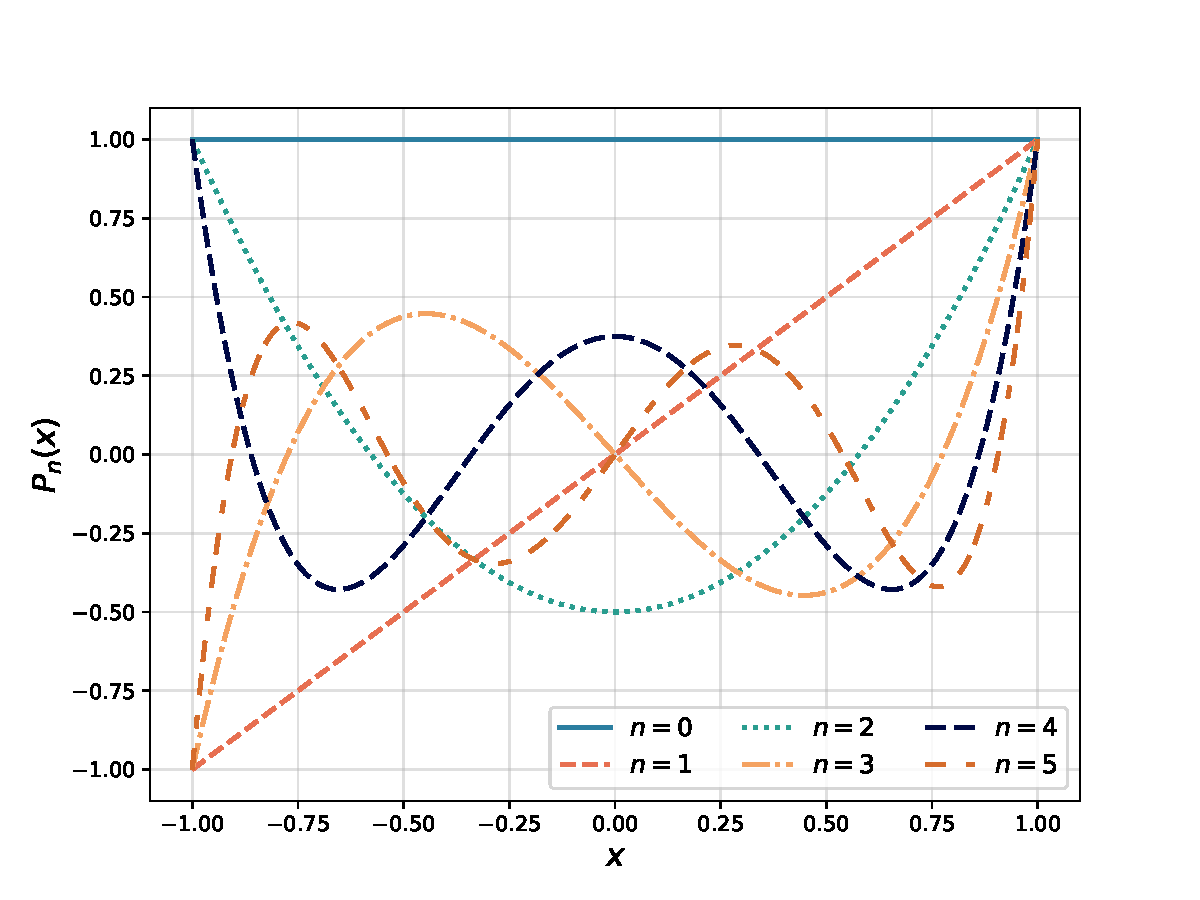
\includegraphics[width=12cm]{./Figuras/Legendre-Polynomials.pdf}
    \caption{Primeros seis polinomios de Legendre. Adaptación de \href{https://github.com/gfrubi/FM2/blob/master/figuras-editables/fig-Legendre.py}{este} código. La adaptación se encuentra \href{https://github.com/Pedroga-cc/Fisica-Matematica-II/blob/main/Figuras/Plotter_Legendre.py}{aquí}.}
    \label{fig:Legendre}
\end{figure}

\subsection{Función Generatriz}

\begin{defi}\marginnote{Función Generatriz}
    Para cualquier conjunto de \emph{polinomios ortogonales} $\{P_n(x)\}_{n\in \mathbb{N}}$, se denomina \textbf{función generatriz} (o generadora) de dicho conjunto a la función $G(x,t)$, tal que al ser desarrollada en una serie de Taylor para $t$, los coeficientes de dicha expansión son los polinomios $P_n(x)$:
\begin{equation}
    G(x,t) = \sum_{n=0}^{\infty} P_n(x)t^n \ .
\end{equation}
\end{defi}

En particular, la función generatriz para los polinomios de Legendre es dada por la expresión
\begin{equation}
    G(x,t) = \frac{1}{\sqrt{1-2xt + t^2}} \ .
\end{equation}
Si observamos esta expresión en detalle, y hacemos $t=r/a$ y $x = \cos\theta$, podemos escribir la función generatriz como
\begin{equation}
    G(\theta, r) = \frac{1}{\sqrt{1-2r \cos(\theta)/a + r^2/a^2}} = \frac{a}{\sqrt{a^2-2ar\cos\theta + r^2}} = \frac{a}{|\vec{x}-\vec{a}|} \ , 
\end{equation} 
donde $|\vec{x}-\vec{a}|$ es la distancia entre los puntos $\vec{x}$ y $\vec{a}$. Así, obtenemos la relación entre la distancia entre dos puntos del espacio con los Polinomios de Legendre,
\begin{equation} \label{eq:Legendre_distancias}
    \frac{1}{|\vec{x} - \vec{a}|} = \frac{1}{a}\sum_{\ell=0}^\infty \left( \frac{r}{a} \right)^\ell P_\ell(\cos\theta) \ .
\end{equation} 
En esta expresión, hemos asumido que $r>a$. En caso contrario, deben invertirse las relaciones dentro de la suma, ubicando $r$ en el lugar de $a$, y viceversa.

\begin{ejemplo}
    Expanda la expresión para un potencial electrostático generado por una carga puntual $q$ en la posición $\vec{a}$ en la región $r < a$.

    \textbf{Solución.} Recordamos que el potencial electrostático debido a una carga puntual es dado por
    \begin{equation}
        \phi(\x) = \frac{1}{4\pi \epsilon_0} \frac{q}{|\x - \vec{a}|} \ .
    \end{equation}

    Reemplazando el resultado obtenido en \eqref{eq:Legendre_distancias}, tenemos que
    \begin{equation}
        \phi(\vec{r}) = \frac{q}{4\pi \epsilon_0 r} \sum_{\ell=0}^\infty \left( \frac{a}{r} \right)^\ell P_\ell(\cos\theta) \ .
    \end{equation}

    La importancia de este resultado es que es la base de la llamada \emph{expansión multipolar}, que estudiarán detalladamente en su curso de electrodinámica.
\end{ejemplo}

% Podemos utilizar este resultado, por ejemplo, para escribir el potencial electrostático en un punto $\vec{r}$ producido por una carga $q$ en el punto $\vec{a}$,

% lo que se asocia a la llamada \emph{expansión multipolar}, que estudiarán en su curso de electrodinámica.

A partir de su función generadora, podemos encontrar explícitamente los polinomios de Legendre mediante la relación
\begin{equation}
    P_n(x) = \frac{1}{n!} \left[ \frac{\partial ^n G(t,x)}{\partial t^n}  \right]_{t=0} \ .
\end{equation}

\subsection{Propiedades}

\begin{propiedad}
    \textbf{Propiedades de los polinomios de Legendre.}

    \begin{enumerate}
        \item \textbf{Normalización.} Los polinomios de Legendre son funciones normalizadas, de modo que $P_n(1) = 1$, para cualquier valor de $n$.
        \item \textbf{Paridad.} Podemos encontrar que los polinomios de Legendre pueden ser funciones pares o impares según el valor de $n$, ya que
        \begin{equation}
            P_n(-x) = (-1)^n P_n(x) \ . 
        \end{equation}
    
        \item \textbf{Valor en el origen.} A partir de la función generatriz, podemos mostrar que
        % propiedad de paridad, podemos observar que, como los polinomios son \emph{impares} para $n$ impar, deberá cumplirse que $P_n(0) = 0$, para $n$ impar. Por otro lado, utilizando la función generatriz, podemos obtener que si $n$ es par, entonces
        \begin{equation}
            P_n(0) = \begin{dcases}
                0 \ , \qquad \text{si } n \text{ es impar.} \\
                (-1)^{n/2} \frac{n!}{2^n ((n/2)!)^2} \ , \qquad \text{si } n \text{ es par.}
            \end{dcases}
        \end{equation}
    
        \item \textbf{Ortogonalidad.} Los polinomios de Legendre satisfacen la relación de ortogonalidad
        \begin{equation}
            \int\limits_{-1}^1 P_n(x) P_m(x) dx = \frac{2}{2n+1} \delta_{n,m} \ .
        \end{equation}
    
        \item \textbf{Completitud.} Los polinomios de Legendre forman un \emph{conjunto completo} de funciones definidas en $[-1,1]$, por lo que forma una base para dichas funciones, lo que se expresa como
        \begin{equation}
            \sum_{n=0}^\infty \frac{2n+1}{2} P_n(x) P_n(x') = \delta(x-x') \ .
        \end{equation}
    
        \item \textbf{Serie de Fourier-Legendre.} Dado que los polinomios de Legendre forman una base en el intervalo $[-1,1]$, podemos expandir cualquier función en una Serie de Fourier-Legendre, tal que
    
        \begin{equation}
            f(x) = \sum_{n=0}^\infty a_n P_n(x) \ ,
        \end{equation}
        donde 
        \begin{equation}
            a_n = \frac{2n+1}{2} \int_{-1}^1 f(x) P_n(x) dx \ .
        \end{equation}
         
        \item \textbf{Relaciones de recurrencia.} Los polinomios de Legendre satisfacen las siguientes relaciones de recurrencia,
        \begin{align}
            n P_{n-1}(x) + (n+1) P_{n+1}(x) & = (2n+1) x P_n(x) \ , \\
            (2n+1) P_n(x) & = P'_{n+1}(x) - P'_{n-1}(x) \ .
        \end{align}    
    \end{enumerate}
\end{propiedad}

\begin{ejemplo}
    \textbf{(Arfken 15.2.2.)} Considere una esfera conductora sin carga de radio $r_0$ que es ubicada en un campo eléctrico uniforme de magnitud $E_0$, como se observa en la figura. Encuentre el nuevo potencial electrostático, perturbado por la ubicación de la esfera, y que satisface la ecuación de Laplace $\nabla^2 \psi = 0$.    

    \begin{center}
    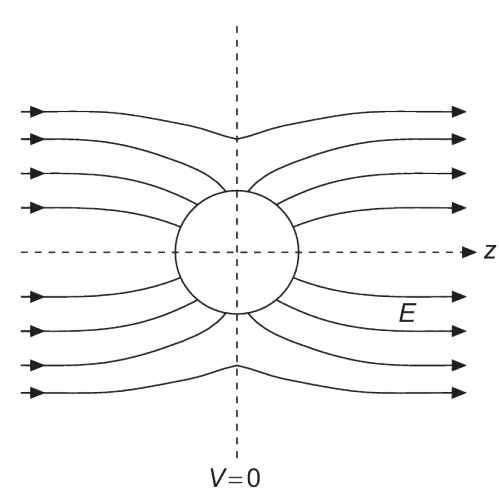
\includegraphics[width = 6cm]{Figuras/Ejemplo-esfera-conductora-2.png}
    \end{center}

    \textbf{Solución.} Trabajaremos en coordenadas esféricas con el origen en el centro de la esfera y el eje $z$ orientado paralelamente al campo uniforme original. Recordemos que el potencial electrostático es una función \emph{continua}, de modo que en la frontera entre el interior y el exterior de la esfera (es decir, en $r = r_0$) la función potencial interior deberá tener el mismo valor que la función potencial exterior.
    
    Dado que la esfera es conductora, esta es \emph{equipotencial}, lo que significa que el potencial es el mismo en todo su volumen, tal que $\psi(r \leq r_0) = V_0$. En particular, dado que la esfera no está cargada, $V_0 = 0$. Supondremos también que en el plano $\theta = \pi/2$, $V = 0$. Esta será nuestra primera condición de borde.

    Separando variables, obtendremos una ecuación radial con soluciones $a_\ell r^\ell + b_\ell r^{-\ell-1}$, y una ecuación axial que corresponde a la ecuación de Legendre. Dada la simetría esférica del sistema, se ha asumido que $m=0$, de modo que la ecuación azimutal da origen a una constante. De este modo, nuestro potencial tendrá la forma
    \begin{equation*}
        \psi(r, \theta) = \sum_{\ell = 0}^\infty \left( a_\ell r^\ell + b_\ell r^{-\ell-1} \right) P_\ell(\cos \theta) \ , \quad r > r_0 \ .
    \end{equation*}

    El efecto de insertar la esfera en el campo eléctrico es local, por lo que el potencial electrostático \emph{muy lejos} de la esfera deberá comportarse como si el campo siguiera siendo uniforme,
    \begin{equation*}
        \psi(r \to \infty, \theta) = - E_0 z = -E_0 r \cos \theta = - E_0 r P_1(\cos \theta) \ ,
    \end{equation*}
    que será nuestra segunda condición de borde. Esta corresponde al caso en que nuestra serie satisface
    \begin{equation*}
        a_1 = -E_0 \ , \qquad a_n = 0 \ , n > 1 \ .
    \end{equation*}

    ¿Por qué es relevante esta elección? Si considerásemos que, por ejemplo, $a_2 \neq 0$, tendríamos términos cuadráticos que dominarían el comportamiento del potencial, de modo que la segunda condición de borde no se estaría satisfaciendo.

    Volviendo a nuestra primera condición de borde, estudiemos el comportamiento de la función en $r = r_0$ y $\theta = \pi/2$. tendremos
    \begin{equation*}
        \psi(r = r_0, \theta = \pi/2) = \frac{b_0}{r_0} + \left( \frac{b_1}{r_0^2} - E_0 r_0 \right) P_1 (\cos \theta) + \sum_{\ell=2}^\infty b_\ell \frac{P_\ell (\cos \theta)}{r_0^{\ell+1}} = 0 \ .
    \end{equation*}

    Esta igualdad se satisface si $b_n = 0$ para $n > 2$. Dado que la esfera no se encuentra cargada, $b_0 = 0$. Por último, despejando $b_1$, encontramos que su valor es
    \begin{equation*}
        b_1 = E_0 r_0^3 \ .
    \end{equation*}

    Así, el potencial electrostático en el exterior de la esfera tendrá la forma
    \begin{equation*}
        \psi_{\text{ext}}(r, \theta) = -E_0 r P_1(\cos \theta) + \frac{E_0 r_0^3}{r^2} P_1(\cos\theta) = - E_0 r \left(1 - \frac{r_0^3}{r^3} \right) P_1 (\cos \theta) \ .
    \end{equation*}

\end{ejemplo}

\subsection{Funciones de Legendre de segunda especie}

Como discutimos anteriormente, al escoger $\lambda = n(n+1)$ para un número entero $n$, debemos truncar una de las series que aparecen en la ecuación \eqref{eq:Legendre_series_solution}, de modo que la solución se reduce a los polinomios de Legendre. El motivo de hacer esto es hallar una solución que converja en $x = \pm 1$. Sin embargo, ¿debemos hacer esto si nuestro problema no requiere convergencia en los contornos $x = \pm 1$?

\begin{defi}\marginnote{Funciones de Legendre de segunda especie}
    Las soluciones a la ecuación de Legendre \eqref{eq:legendre_explicit} que no son convergentes en los puntos $x = \pm 1$ son llamadas \textbf{funciones de Legendre de segunda especie}, denotadas por $Q_n(x)$. Estas se definen como
    \begin{align} \label{eq:legendre-second-kind}
        Q_n(x) & = \begin{dcases}
            d_{1,n} y_{2,n}(x) \ , \qquad \text{ si } n \text{ es par} \ , \\
            d_{2,n} y_{1,n}(x) \ , \qquad \text{ si } n \text{ es impar} \ ,
        \end{dcases} \\
        & = \left\{ \begin{array}{cc}
            (-1)^{n/2} \dfrac{[(n/2)!]^2}{n!} 2^n y_{2,n}(x) , & \text{ si } n \text{ es par} \ , \\
            (-1)^{(n+1)/2} \dfrac{[\left((n-1)/2\right)!]^2}{n!} 2^{n-1} y_{1,n}(x) \ , & \text{ si } n \text{ es impar} \ ,
        \end{array} \right.
    \end{align}
    donde $y_{1,n}$ e $y_{2,n}$ son las funciones definidas en \eqref{eq:y1n_legendre} y \eqref{eq:y2n_legendre}, respectivamente. 
    
    Nótese que \emph{a la solución para} $n$ \emph{par, hemos multiplicado los coeficientes de la solución impar}, y viceversa.
\end{defi}

% La respuesta es no, y de hecho ciertos problemas físicos requieren de estas soluciones. Por ello, las llamaremos \textbf{funciones de Legendre de segunda especie}, denotadas por $Q_n(x)$, y que definimos como
% \begin{align}
%     Q_n(x) & = \begin{dcases}
%         d_{1,n} y_{2,n}(x) \ , \qquad \text{ si } n \text{ es par} \ , \\
%         d_{2,n} y_{1,n}(x) \ , \qquad \text{ si } n \text{ es impar} \ ,
%     \end{dcases} \\
%     & = \begin{dcases}
%         (-1)^{n/2} \frac{[(n/2)!]^2}{n!} 2^n y_{2,n}(x) \ , \qquad \text{ si } n \text{ es par} \ , \\
%         (-1)^{(n+1)/2} \frac{[\left(\frac{n-1}{2}\right)!]^2}{n!} 2^{n-1} y_{1,n}(x) \ , \qquad \text{ si } n \text{ es impar} \ ,
%     \end{dcases}
% \end{align}
% donde $y_{1,n}$ e $y_{2,n}$ son las funciones definidas en \eqref{eq:y1n_legendre} y \eqref{eq:y2n_legendre}, respectivamente. Nótese que \emph{a la solución para} $n$ \emph{par, hemos multiplicado los coeficientes de la solución impar}, y viceversa.

Las funciones asociadas de Legendre satisfacen las mismas relaciones de recurrencia que las funciones de Legendre, de modo que
\begin{align}
    nQ_{n-1}(x) + (n+1)Q_{n+1}(x) & = (2n+1) x Q_n(x) \ , \\
    (2n+1)Q_n(x) & = Q'_{n+1}(x) - Q'_{n-1}(x) \ . 
\end{align}
Gracias a ellas, podemos obtener las expresiones explícitas para funciones de orden superior, debiendo utilizar la definición \eqref{eq:legendre-second-kind} únicamente para las funciones $Q_0(x)$ y $Q_1(x)$. Pueden encontrar estas derivaciones en el capítulo 5 de \cite{Rubilar}.

Las primeras seis funciones de Legendre de segunda especie son graficadas en la figura \ref{fig:Legendre-second-kind}, y las expresiones para las primeras cuatro son dadas por

\begin{minipage}[b]{.45\textwidth}
    \begin{align*}
        Q_0(x) & = \frac{1}{2} \ln\left( \frac{1+x}{1-x} \right) \ , \\
        Q_1(x) & = \frac{x}{2} \ln\left( \frac{1+x}{1-x} \right) - 1 \ ,
    \end{align*}
\end{minipage}
\hfill
\begin{minipage}[b]{.5\textwidth}
    \begin{align*}
        Q_2(x) & = \frac{3x^2-1}{4}\ln\left( \frac{1+x}{1-x} \right) - \frac{3x}{2} \ , \\
        Q_3(x) & = \frac{5x^3 - 3x}{4}\ln\left( \frac{1+x}{1-x} \right) - \frac{5x^2}{2} + \frac{2}{3} \ . 
    \end{align*}
\end{minipage}

\begin{figure}[htbp]
    \centering
    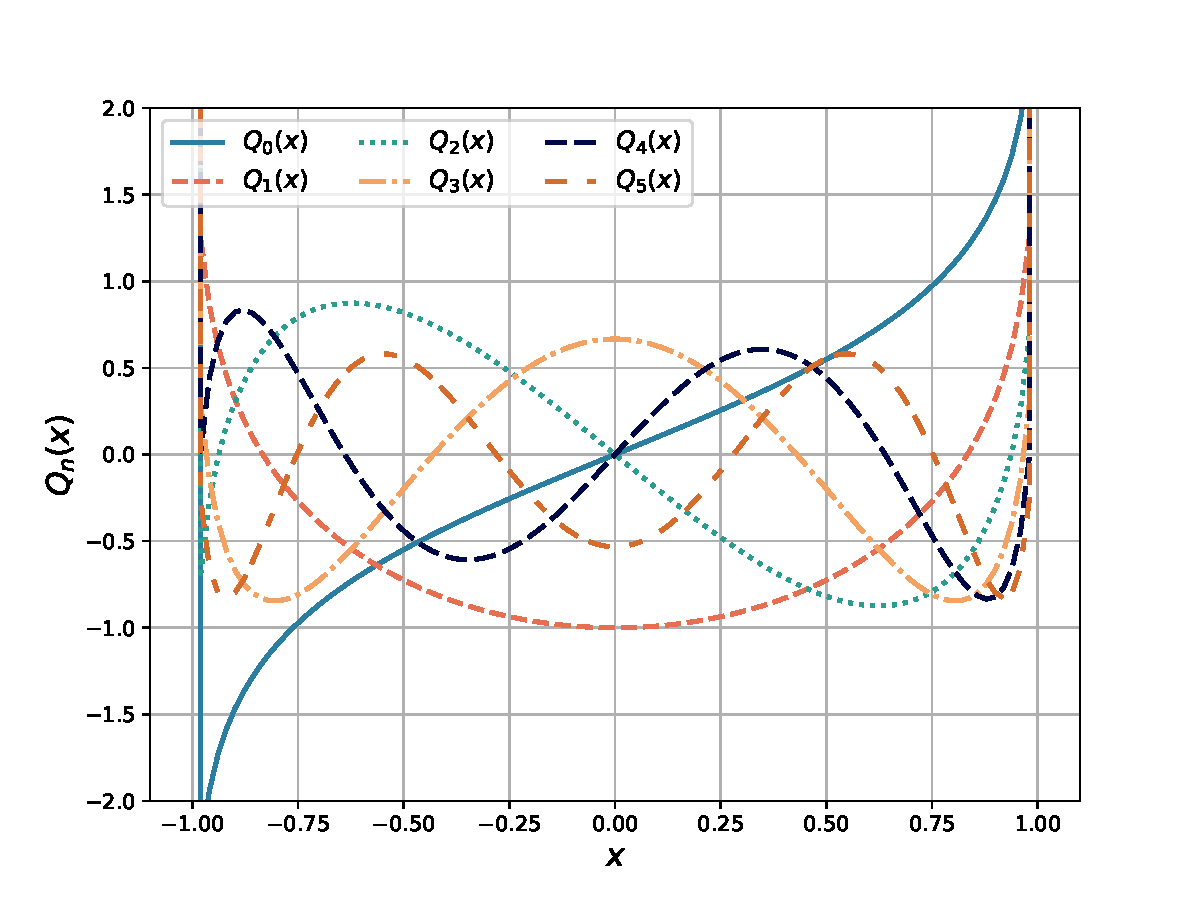
\includegraphics[width=12cm]{Figuras/Legendre-second-kind.pdf}
    \caption{Primeras seis funciones de Legendre de segunda especie. Nótese el comportamiento asintótico alrededor de los extremos $x = -1$ y $x=1$. Adaptación de \href{https://github.com/gfrubi/FM2/blob/master/figuras-editables/fig-Legendre.py}{este} código. La adaptación se encuentra \href{https://github.com/Pedroga-cc/Fisica-Matematica-II/blob/main/Figuras/Plotter_Legendre.py}{aquí}.}
    \label{fig:Legendre-second-kind}
\end{figure}

\begin{propiedad}
    \textbf{Propiedades de las funciones de Legendre de segunda especie.}

    \begin{enumerate}
        \item \textbf{Paridad.} Se tiene que
        \begin{equation}
            Q_n(-x) = (-1)^{n+1} Q_n(x) \ .
        \end{equation}
        \item \textbf{Valor en el origen.} Dada su paridad, las relaciones se invierten respecto a los polinomios de Legendre, de modo que
        \begin{equation}
            Q_n(0) = \begin{dcases}
                0 \ , \qquad \text{si } n \text{ es par} \ , \\
                (-1)^{(n+1)/2} \frac{\left[ \left( \frac{n-1}{2} \right)! \right]^2}{n!} 2^{n-1} \ , \qquad \text{si } n \text{ es impar} \ .  
            \end{dcases}
        \end{equation}
        \item \textbf{Valor en el extremo del intervalo.} Los extremos del intervalo son puntos singulares para estas funciones, de modo que
        \begin{equation}
            \lim_{x \to 1} Q_n(x) = +\infty \ .
        \end{equation}
    \end{enumerate} 
\end{propiedad}

% Otras propiedades relebvantes que estas satisfacen son


En resumen, la solución general de la EDO de Legendre para $\lambda = n(n+1)$, es dada por
\begin{equation}
    y(x) = C_1 P_n(x) + C_2 Q_n(x) \ ,
\end{equation}
donde los polinomios de Legendre $P_n(x)$ convergen en todo el intervalo $[-1,1]$, incluídos los extremos, mientras que las funciones de segunda especie $Q_n(x)$ convergen en el interior del intervalo $(-1,1)$, mas no en los extremos.

\begin{obs}{Observación}
    Si bien lo más adecuado es plantear siempre la solución a la EDO de Legendre considerando las funciones de primera y segunda especie, la gran mayoría de problemas físicos descartarán la solución de segunda especie, dada su divergencia en los extremos.

    La referencia \cite{Lebedev_Silverman_1972} plantea que las funciones de segunda especie aparecerán en problemas poco comunes, como el campo electrostático en un conductor toroidal, o en la atracción gravitacional ejercida por un esferoide sólido, entre otras. Puede revisar el capítulo 8 de esa referencia para más detalles.
\end{obs}

\section{Ecuación y funciones asociadas de Legendre}

Hasta ahora, analizamos el caso en que $m=0$ en la EDO axial \eqref{eq:Helmholtz_esferica} que se obtiene de la ecuación de Helmholtz. En lo que resta del capítulo, analizaremos el caso en que $m \neq 0$.

En este caso, bajo el cambio de variable $x=\cos\theta$, la ecuación \eqref{eq:Helmholtz_esferica} toma la forma de la 
% \begin{equation}
%     \frac{1}{\sin\theta} \frac{d}{d\theta}\left( \sin\theta \frac{d\Theta}{d\theta} \right) + \left(\lambda - \frac{m^2}{\sin^2\theta} \right) \Theta = 0 \ .
% \end{equation}
%
% Realizando nuestro cambio de variable $x = \cos\theta$, y desarrollando de forma más explícita la ecuación, esta toma la forma de la 
\textbf{ecuación asociada de Legendre},
\begin{equation}\label{eq:EDO_asociada_Legendre}
    (1-x^2) \frac{d^2y}{dx^2} - 2x\frac{dy}{dx} + \left( \lambda - \frac{m^2}{1-x^2} \right) y = 0 \ ,
\end{equation}
cuyas soluciones se encuentran definidas en el intervalo $[-1,1]$.

\subsection{Resolviendo la ecuación asociada de Legendre}

Para hacer más fácil el proceso de utilizar el método de series, realizamos la sustitución $y(x) = (1-x^2)^{m/2} u(x)$, de modo que
\begin{align*}
    y'(x) & = \frac{\left(1 - x^{2}\right)^{\frac{m}{2}} \left((1 - x^2) u'\left(x\right) - mx u\left(x\right)\right)}{1 - x^2} \\
    %  -m x (1-x^2)^{m/2 - 1} u(x) + (1-x^2)^{m/2} u'(x) \\
    y''(x) & = \frac{\left(1 - x^{2}\right)^{\frac{m}{2}} \left[(1-x^2)^2 u'' \left(x\right) - 2mx (1 - x^2) u'(x) + m\left((m - 1) x^{2} - 1\right) u\left(x\right)\right]}{(1- x^2)^2} \ .
\end{align*}

Reemplazamos esta función y sus derivadas en \eqref{eq:EDO_asociada_Legendre}, de modo que
\begin{align*}
    (1-x^2)\frac{\left(1 - x^{2}\right)^{\frac{m}{2}} \left[(1-x^2)^2 u'' \left(x\right) - 2mx (1 - x^2) u'(x) + m\left((m - 1) x^{2} - 1\right) u\left(x\right)\right]}{(1- x^2)^2} & \\
    - 2x \frac{\left(1 - x^{2}\right)^{\frac{m}{2}} \left((1 - x^2) u'\left(x\right) - mx u\left(x\right)\right)}{1 - x^2} + \left(\lambda - \frac{m^2}{1-x^2}\right) (1-x^2)^{m/2} u(x) & = 0 \\
    % \frac{\left[(1-x^2)^2 u'' \left(x\right) - 2mx (1 - x^2) u'(x) + m\left((m - 1) x^{2} - 1\right) u\left(x\right)\right]}{(1- x^2)} - 2x & \\
    % \frac{\left((1 - x^2) u'\left(x\right) - mx u\left(x\right)\right)}{1 - x^2} + \left(\lambda - \frac{m^2}{1-x^2}\right) (1-x^2)^{m/2} u(x) + \left(\lambda - \frac{m^2}{1-x^2}\right) u(x) & = 0 \\
    (1-x^2) u''(x)  - 2m (x + 1) u'(x) + \left[ \left( \lambda - \frac{m^2}{1-x^2} \right) + \frac{2mx + m[(m-1)x^2 - 1]}{1-x^2} \right]u(x) & = 0 \\
    (1-x^2) u''(x)  - 2m (x + 1) u'(x) + \left[ \frac{\lambda(1-x^2) - m(m+1)(1-x^2)}{1-x^2} \right]u(x) & = 0 \,
\end{align*}
%
% \hrule
%
% AA
%
% \hrule
%
lo que resulta en la EDO para $u(x)$
\begin{equation}
    (1-x^2)u''(x) - 2x(m+1)u'(x) + (\lambda - m(m+1))u(x) = 0 \ .
\end{equation}

En este caso, $P(x) = 2x(m+1)/(1-x^2)$ y que $Q(x) = (\lambda - m(m+1))/(1-x^2)$, de modo que como ambas funciones son analíticas en $x=0$, podemos plantear una solución de la forma
\begin{equation}
    u(x) = \sum_{k=0}^{+\infty} a_k x^k 
\end{equation} 
que nos llevará a la relación de recurrencia
\begin{equation}\label{eq:recurrencia_asociadas}
    a_{k+2} = \frac{k^2 + (2m+1)k - \lambda + m(m+1)}{(k+1)(k+2)} a_k \ ,
\end{equation}
que al igual que para la ecuación de Legendre, resultará en series que convergen para $|x|<1$ y, en general, divergen para $|x|=1$, salvo para ciertos valores de $\lambda$. Para encontrar dichos valores, necesitamos que el numerador de la ecuación \eqref{eq:recurrencia_asociadas} sea cero. Esto impone que $\lambda$ debe satisfacer la igualdad
\begin{equation}
    \lambda = m(m+1) + k(k+1) + 2mk = (m+k)(m+k+1) \ ,
\end{equation}
y definiendo $n = m+k \geq m$, observamos que nuevamente requeriremos que $\lambda = n(n+1)$, de modo que la serie se truncará luego del $(n-m)$-ésimo término.

Podemos hallar de forma explícita las soluciones a esta EDO diferenciando repetidamente la ecuación de Legendre \eqref{eq:legendre_explicit}, al hacer uso de la regla de Leibniz, es decir,
\begin{equation}
    \frac{d^m}{dx^m}\left( f_1(x) \cdot f_2(x) \right) = \sum_{s=0}^{m} \binom{m}{s} \frac{d^{m-s}f_1(x)}{dx^{m-s}} \frac{d^s f_2(x)}{dx^s} \ ,
\end{equation}
de donde obtenemos que
\begin{align*}
    \frac{d^m}{dx^m}\left[ (1-x^2)y'' \right] & = \binom{m}{m} (1-x^2) \frac{d^m y''}{dx^m} - \binom{m}{m-1} 2x \frac{d^{m-1} y''}{dx^{m-1}}  - \binom{m}{m-2} 2 \frac{d^{m-2} y''}{dx^{m-2}} \\
    & = (1-x^2) \left(\frac{d^m y}{dx^m}\right)'' - 2mx \left(\frac{d^m y}{dx^m}\right)' - m(m-1)\left(\frac{d^m y}{dx^m}\right)  \\
    \frac{d^m}{dx^m}\left[ 2x y' \right] & = \binom{m}{m} 2x \frac{d^m y'}{dx^m} + \binom{m}{m-1} 2 \frac{d^{m-1} y'}{dx^{m-1}} \\
    & = 2x \left(\frac{d^2 y}{dx^2}\right)' + 2m \left(\frac{d^2 y}{dx^2}\right) \\
    \frac{d^m}{dx^m}\left[ n(n+1)y \right] & = n(n+1) \frac{d^m y}{dx^m} \ ,
\end{align*}
donde hemos usando que $\binom{m}{m} = 1$, $\binom{m}{m-1} = m$, y $\binom{m}{m-2} = \frac{m(m-1)}{2}$. Así, la EDO resulta en
\begin{align*}
    (1-x^2)\left(\frac{d^m y}{dx^m}\right)'' - (2mx + 2x) \left(\frac{d^m y}{dx^m}\right)' + [m(m-1) + 2m + n(n+1)]\left(\frac{d^m y}{dx^m}\right) & = 0 \\
    (1-x^2)\left(\frac{d^m y}{dx^m}\right)'' - 2x(m + 1) \left(\frac{d^m y}{dx^m}\right)' + [m(m+1) + n(n+1)]\left(\frac{d^m y}{dx^m}\right) & = 0 \ , 
\end{align*}
donde al hacer la sustitución $f(x) = y^{(m)}(x)$, obtenemos la EDO para $u(x)$ cuando $\lambda = n(n+1)$. De esta forma, concluímos que las funciones $u(x)$ deberán ser proporcionales a $\frac{d^m }{dx^m} P_n(x)$.

\begin{defi}\marginnote{Polinomios asociados de Legendre}
    Se definen los \textbf{polinomios asociados de Legendre}, soluciones de la EDO \eqref{eq:EDO_asociada_Legendre}, como
    \begin{equation} \label{eq:asociadas_legendre}
        P_n^m(x) = (1-x^2)^{m/2} \frac{d^m}{dx^m}P_n(x) \ ,
    \end{equation}
    donde el factor $(1-x^2)^{m/2}$ es introducido para una correcta normalización. Nótese que cuando $m=0$, se recuperan los polinomios de Legendre \eqref{eq:Legendre_series_solution}, de modo que $P_n^0(x) \equiv P_n(x)$. 

    También se admite la definición mediante la fórmula de Rodrigues
    \begin{equation} \label{eq:rodrigues-asociados}
        P_n^m(x) = \frac{1}{2^n n!}(1-x^2)^{m/2} \frac{d^{n+m}}{dx^{n+m}}(x^2-1)^n \ ,
    \end{equation}
    obtenida al sustituir la fórmula de Rodrigues para los polinomios de Legendre en la ecuación \eqref{eq:asociadas_legendre}, y es también válida para $m<0$, siempre y cuando $|m|\leq n$.
\end{defi}

% De forma convencional (por motivos de normalización), las soluciones $u(x)$ corresponden a los \textbf{polinomios asociadas de Legendre}, expresados como
% \begin{equation} \label{eq:asociadas_legendre}
%     P_n^m(x) = (1-x^2)^{m/2} \frac{d^m}{dx^m}P_n(x) \ .
% \end{equation}

% Observamos que cuando $m=0$, recuperamos los polinomios de Legendre, de modo que $P^0_n(x) \equiv P_n(x)$. Sustituyendo la fórmula de Rodrigues para $P_n(x)$ en \eqref{eq:asociadas_legendre}, obtenemos la \emph{fórmula de Rodrigues para los polinomios asociados de Legendre},
% \begin{equation} \label{eq:rodrigues-asociados}
%     P_n^m(x) = \frac{1}{2^n n!}(1-x^2)^{m/2} \frac{d^{n+m}}{dx^{n+m}}(x^2-1)^n \ ,
% \end{equation}
% que también es válida para $m<0$, siempre y cuando $|m|\leq n$.

\subsection{Función generatriz}

En este caso, podemos hacer uso de la relación entre los polinomios asociados de Legendre y los polinomios de Legendre para obtener la función generatriz de los primeros. En efecto, observamos que derivando $m$ veces la función generatriz de los polinomios de Legendre respecto a $x$, tenemos
\begin{equation}
    \frac{d^m G}{dx^m} = \frac{d^m}{dx^m}(1-2xt+t^2)^{-1/2} = \sum_{n=0}^\infty \frac{d^m}{dx^m}P_n(x) t^n \ ,
\end{equation}
y multiplicando ambos lados por $(1-x^2)^{m/2}$, tenemos que
\begin{equation}
    \frac{d^m G}{dx^m} = (1-x^2)^{m/2} \frac{d^m}{dx^m}(1-2xt+t^2)^{-1/2} = \sum_{n=0}^\infty P^m_n(x) t^n \ .
\end{equation}

Derivando el lado izquierdo de la ecuación, obtenemos
\begin{equation}
    \frac{1 \cdot 3 \cdot 5 \dots (2m-1) (1-x^2)^{m/2} t^m}{(1-2xt+t^2)^{m+1/2}} = \sum_{n=0}^\infty P_n^m t^n \ .
\end{equation}
Dividimos la expresión por $t^m$, definimos una variable auxiliar $r=n-m$, y además notamos que
\begin{equation}
    1 \cdot 3 \cdot 5 \dots (2r-1) = \frac{1 \cdot 2 \cdot 3 \dots 2r}{2 \cdot 4 \cdot 6 \dots 2r} = \frac{(2r)!}{2^r r!} \ .
\end{equation}

De este modo, podemos hallar que
\begin{equation}
    G_m(x,t) = \frac{(2m)! (1-x^2)^{m/2}}{2^m m! (1-2xt+t^2)^{m+1/2}} = \sum_{r=0}^\infty P_{r+m}^m(x) t^r \ .
\end{equation}

\subsection{Propiedades}

\begin{propiedad}
    \textbf{Propiedades de los polinomios asociados de Legendre.}

    % A partir de la expresión \eqref{eq:asociadas_legendre}, es posible mostrar, aplicando la fórmula de Leibniz al producto $(n+1)^n (x-1)^n$, que
    \begin{enumerate}[series=asociadas]
        \item \textbf{Simetría.} Los polinomios $P^{-m}_n$ se pueden obtener a partir de los $P^{m}_n$ siguiendo la relación
        \begin{equation}
            P^{-m}_n(x) = (-1)^m \frac{(n-m)!}{(n+m)!}P^{m}_n(x) \ .
        \end{equation}
        Esto se puede demostrar a partir de la expresión \eqref{eq:asociadas_legendre}, aplicando la fórmula de Leibniz al producto $(n+1)^n (x-1)^n$.
    \end{enumerate}

    A partir de la fórmula de Rodrigues \eqref{eq:rodrigues-asociados}, se pueden demostrar las siguientes propiedades,
    \begin{enumerate}[resume=asociadas]
        \item \textbf{Valor en los extremos.} Evaluados en los extremos del intervalo $x= \pm 1$, los polinomios asociados de Legendre son nulos, salvo cuando $m=0$.
        \begin{equation}
            P_n^m(\pm 1) = \begin{dcases}
                (\pm 1)^n \ , & \qquad m = 0 \\
                0 \ , & \qquad m \neq 0
            \end{dcases} \ .
        \end{equation}

        \item \textbf{Paridad.} A partir de la paridad de los polinomios de Legendre $P_n(x)$, podemos encontrar que los polinomios asociados pueden ser tanto funciones pares como impares, dependiendo del valor de $m$ y $n$,
        \begin{equation}
            P_n^m(-x) = (-1)^{n+m} P_n^m(x) \ .
        \end{equation}

        \item \textbf{Ortogonalidad.} Los polinomios asociados de Legendre satisfacen las siguientes relaciones de ortogonalidad,
        \begin{gather}
            \int_{-1}^1 P_\ell^m(x) P_k^m(x) \, dx = \int_0^\pi P_\ell^m(\cos\theta) P_k^m(\cos\theta) \sin\theta \, d\theta = \frac{2}{2\ell + 1} \frac{(\ell + m)!}{(\ell - m)!} \delta_{\ell, k} \ , \\
            \int_{-1}^1 P_\ell^m(x) P_\ell^n(x) \frac{dx}{1-x^2} = \int_0^\pi P_\ell^m(\cos\theta) P_\ell^n(\cos\theta) \frac{d\theta}{\sin \theta} = \frac{(\ell+m)!}{m(\ell-m)!} \delta_{m,n} \ .
        \end{gather}

        \item \textbf{Relaciones de recurrencia.} Los polinomios asociados de Legendre satisfacen las siguientes relaciones de recurrencia,
        \begin{align}
            (2n+1)x P_n^m(x) & = (n+m) P^m_{n-1}(x) + (n-m+1) P^m_{n+1}(x) \ , \\
            (2n+1) \sqrt{1-x^2} P_n^m(x) & = P^{m+1}_{m+1}(x) - P^{m+1}_{n-1}(x) \\
            & = (n+m)(n+m-1)P^{m-1}_{n-1} \nonumber \\
            & \quad - (n-m+1)(n-m+2)P^{m-1}_{n+1} \ .
        \end{align}

        \item En general, la EDO asociada de Legendre también posee un segundo conjunto de soluciones, no analíticas en $x = \pm 1$, que corresponden a las \emph{funciones asociadas de Legendre de segunda especie}, que se obtienen a partir la ecuación \eqref{eq:asociadas_legendre}, utilizando las funciones de Legendre de segunda especie $Q_n(X)$ como derivando. Por ello, la solución general será dada por
        \begin{equation}
            y(x) = C_1 P_n^m(x) + C_2 Q_n^m(x) \ .
        \end{equation}

        \item La mayoría de los problemas físicos descartan esta segunda solución, ya que en general esperaremos que nuestra solución sea finita en $x = \pm 1$, es decir, en $\theta = 0$ y en $\theta = \pi$, con lo que hacemos $C_2 = 0$.
    \end{enumerate}
\end{propiedad}

\newpage

\section{Armónicos Esféricos}

Como último tema de este capítulo, analizaremos qué ocurre al resolver la ecuación de Laplace, es decir, el caso en que $k=0$ en la ecuación de Helmholtz. Mediante el método de separación de variables, llegamos a las ecuaciones angulares
\begin{align}
    \frac{d^2 \Phi}{d\phi^2} + m^2 \Phi & = 0 \label{eq:edo_laplace_phi} \\
    \frac{1}{\sin \theta} \frac{d}{d\theta}\left( \sin\theta \frac{d\Theta}{d\theta} \right) + \left( \ell(\ell+1) - \frac{m^2}{\sin^2\theta} \right)\Theta & = 0 \label{eq:edo_laplace_theta} \ ,
\end{align}
y a la ecuación radial
\begin{equation}
    \frac{d}{dr}\left( r^2 \frac{dR}{dr} \right) - \ell(\ell+1) R = 0 \ , \label{eq:edo_laplace_r}
\end{equation}
donde la elección de la constante de separación $\ell(\ell+1)$ proviene de exigir una solución analítica cuando $\cos\theta = \pm 1$. Luego, la solución de la ecuación \eqref{eq:edo_laplace_phi} es oscilante para satisfacer la condición de periodicidad $\Phi(\phi) = \Phi(\phi + 2\pi)$, la solución a la ecuación \eqref{eq:edo_laplace_theta} son los polinomios asociados de Legendre, y la solución para \eqref{eq:edo_laplace_r} es $R_\ell(r) = D_\ell r^\ell + E_\ell r^{-(\ell+1)}$.

Una solución para la ecuación de Laplace en coordenadas esféricas será, por ende,
\begin{align}
    \psi_{m\ell}(r,\theta,\phi) & = R_\ell(r) \Theta_{m\ell}(\theta) \Phi_m (\phi) \nonumber \\
    & = (D_\ell r^\ell + E_\ell r^{-(\ell+1)}) C_{m\ell} P_\ell^m(\cos\theta)(A_m \cos(m\phi) + B_m \sin(m\phi)) \ ,
\end{align}
o bien,
\begin{equation}
    \psi_{m\ell}(r,\theta,\phi) = (D_{\ell, m} r^\ell + E_{\ell, m} r^{-(\ell+1)}) P_\ell^m(\cos\theta) e^{im\phi} \ ,
\end{equation}
donde se cumplirá que $- \ell \leq m \leq \ell$.

Sin embargo, recordemos que en la ecuación de Helmholtz la constante $k$ siempre es separada junto a la variable radial, por lo que nuestra EDO para $R$ podrá tener una forma diferente, pero las ecuaciones para $\phi$ y $\theta$ seguirán siendo las ecuaciones \eqref{eq:edo_laplace_phi} y \eqref{eq:edo_laplace_theta}, respectivamente, por lo que las soluciones serán de la forma
\begin{equation}\label{eq:solucion_armonicos} 
    \psi_{k\ell m}(r, \theta, \phi) = R_{k, \ell}(r) P_\ell^m(\cos\theta) e^{im\phi} \ .
\end{equation}
Incluso, si $k$ no es una constante, sino que una función que depende únicamente de $r$, la solución al problema tendrá la forma \eqref{eq:solucion_armonicos}, de modo que será deseable denotar de alguna forma esta solución \emph{angular} a la ecuación de Helmholtz ``generalizada''.

\begin{defi} \marginnote{Armónicos esféricos}
    Se denominan \textbf{funciones armónicas esféricas} $Y_\ell^m$, o simplemente \textbf{armónicos esféricos}, a las soluciones de la parte angular de la ecuación de Laplace. Son definidos como
    \begin{equation}
        Y_\ell^m(\theta, \phi) = (-1)^m \sqrt{\frac{2\ell + 1}{4\pi} \frac{(\ell-m)!}{(\ell+m)!} } P_\ell^m (\cos\theta) e^{im\phi} \ .
    \end{equation}
    Las constante bajo raíz permite que las funciones se encuentren normalizadas, mientras que el factor $(-1)^m$ es convencional al trabajar en mecánica cuántica en el contexto del momento angular. Esta fase es conocida como \emph{fase de Condon-Shortley}, y a veces es introducida en la definición de los polinomios asociados de Legendre.
\end{defi}

% Comúnmente, nos podemos referir a la parte angular de la solución general como \textbf{funciones armónicas esféricas}, o simplemente, \textbf{Armónicos Esféricos}, los que se definen con una normalización conveniente como
% \begin{equation}
%     Y_\ell^m(\theta, \phi) = (-1)^m \sqrt{\frac{2\ell + 1}{4\pi} \frac{(\ell-m)!}{(\ell+m)!} } P_\ell^m (\cos\theta) e^{im\phi} \ .
% \end{equation}

% El factor radical tiene su origen en la normalización de los armónicos esféricos, mientras que el factor $(-1)^m$ es convencional al trabajar en mecánica cuántica en el contexto del momento angular. Esta fase es conocida como \emph{fase de Condon-Shortley}, y a veces es introducida en la definición de los polinomios asociados de Legendre.

\subsection{Propiedades}

\begin{propiedad}
    \textbf{Propiedades de los armónicos esféricos.}

    \begin{enumerate}
        \item \textbf{Simetría.} Los armónicos esféricos $Y_\ell^{-m}$ se pueden obtener según la relación
        \begin{equation}
            Y_\ell^{-m}(\theta, \phi) = (-1)^m (Y_\ell^m (\theta, \phi))^\ast \ .
        \end{equation}
    
        \item \textbf{Paridad.} Los armónicos esféricos pueden ser pares o impares, según el valor de $\ell$,
        \begin{equation}
            Y_\ell^m(\pi - \theta, \pi + \phi) = (-1)^\ell Y_\ell^m(\theta, \phi) \ .
        \end{equation}
    
        \item \textbf{Ortonormalidad.} Los armónicos esféricos forman un conjunto ortonormal, es decir,
        \begin{equation}
            \int_0^{2\pi} \int_0^\pi \left[Y_j^k(\theta, \phi)\right]^\ast Y_\ell^m (\theta, \phi) \sin\theta d\theta d\phi = \delta_{j, \ell} \delta_{k, m} \ .
        \end{equation}
    
        \item \textbf{Completitud.} EL conjunto de funciones $\{ Y_\ell^m(\theta, \phi) \}_{\ell = 0, m = -\ell}^{\ell = \infty, m = \ell}$ es un \emph{conjunto completo de funciones}, con lo que \emph{forma una base en el espacio de funciones}, lo que se expresa como
        \begin{equation}
            \sum_{\ell = 0}^{\infty} \sum_{m = -\ell}^{\ell} \left[Y_\ell^m (\theta, \phi)\right]^\ast Y_{\ell}^m (\theta', \phi') = \frac{1}{\sin \theta} \delta(\phi - \phi') \delta(\theta - \theta') \ .
        \end{equation}
        
        \item \textbf{Expansión en términos de Armónicos Esféricos.} Dada la completitud de los armónicos esféricos, cualquier función $f(\theta, \phi)$ cuadrado integrable, es decir, que satisface
        \begin{equation}
            \int | f(\theta, \phi) |^2 d\Omega < \infty \ ,
        \end{equation}
        puede ser desarrollada en términos de funciones armónicas esféricas, también llamada \emph{serie de Laplace},
        \begin{equation}
            f(\theta, \phi) = \sum_{\ell = 0}^{\infty} \sum_{m = -\ell}^{\ell} a_{\ell m} Y_\ell^m (\theta, \phi) \ ,
        \end{equation}
        donde los coeficientes $a_{\ell m}$ son dados por
        \begin{equation}
            a_{\ell m} = \int_{0}^{2\pi} \int_{0}^{\pi} f(\theta, \phi) \left[Y_\ell^m (\theta, \phi)\right]^\ast \sin\theta d\theta d\phi \ .
        \end{equation}
    
        \item \textbf{Teorema de adición de armónicos esféricos.} Dados dos vectores unitarios $\hat{r}_1$ y $\hat{r}_2$, con direcciones $(\theta_1, \phi_1)$ y $(\theta_2, \phi_2)$, podemos obtener el ángulo $\gamma$ formado entre ambos vectores como
        \begin{equation}
            \hat{r}_1 \cdot \hat{r}_2 = \cos\gamma = \sin\theta_1 \sin\theta_2 \cos(\phi_1 - \phi_2) + \cos\theta_1 \cos\theta_2 \ ,
        \end{equation}
        donde hemos usado que
        \begin{equation*}
            \hat{r}_i = \sin \theta_i \cos \phi_i \hat{x} + \sin \theta_o \sin \phi_i \hat{y} + \cos \theta_i \hat{z} \ .
        \end{equation*}
        De este modo, podremos hallar los polinomios de Legendre de este ángulo como
        \begin{equation}
            P_\ell(\cos\gamma) = \frac{4\pi}{2\ell + 1} \sum_{m = -\ell}^\ell Y_\ell^m(\theta_1, \phi_1) \left[Y_\ell^m(\theta_2, \phi_2)\right]^\ast \ .
        \end{equation}
    
        En particular, cuando $\gamma=0$, y por ende $\theta_1 = \theta_2 = \theta$ y $\phi_1 = \phi_2 = \phi$, obtenemos que
        \begin{equation}
            P_\ell(1) = 1 = \frac{4\pi}{2\ell + 1} \sum_{m = -\ell}^\ell |Y_\ell^m(\theta, \phi)|^2 \ ,
        \end{equation}
        y así,
        \begin{equation}
            \sum_{m = -\ell}^\ell |Y_\ell^m(\theta, \phi)|^2 = \frac{2\ell + 1}{4\pi} \ .
        \end{equation}

        \begin{center}
            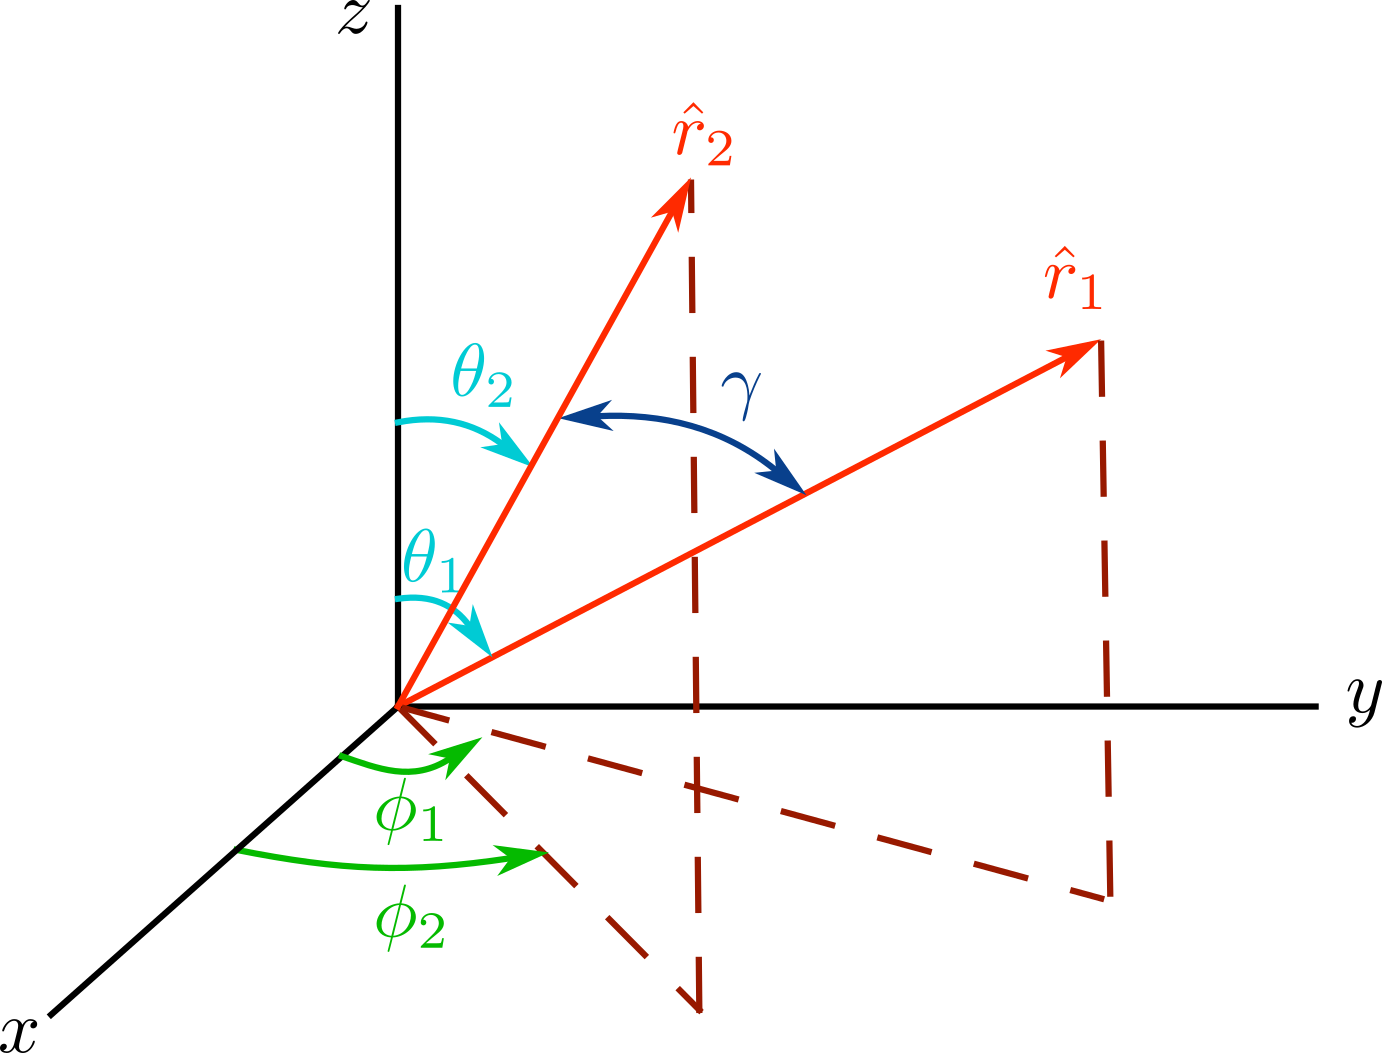
\includegraphics[width=8cm]{Figuras/Addition_Theorem.png}
            \captionof{figure}{Descripción geométrica de los ángulos involucrados en el teorema de adición de armónicos esféricos.}
        \end{center}
       
    
    \end{enumerate}
\end{propiedad}

\begin{ejemplo}
    Dada una partícula cuántica en presencia de un potencial central $V(r)$, su movimiento es descrito por la ecuación de Schrödinger \eqref{eq:schrodinger}, tal que
    \begin{equation*}
        - \frac{\hbar^2}{2m} \left[ \frac{1}{r^2} \frac{\partial}{\partial r} \left( r^2 \frac{\partial}{\partial r} \right) + \frac{1}{r^2 \sin\theta} \frac{\partial}{\partial \theta} \left( \sin \theta \frac{\partial}{\partial \theta} \right) + \frac{1}{r^2 \sin^2\theta} \frac{\partial^2}{\partial \phi^2} + V(r) \right]  \psi = E \psi \ .
    \end{equation*}

    Notemos que, bajo la sustitución
    \begin{equation*}
        k^2 = \frac{2m}{\hbar^2} (V(r) - E) \ ,
    \end{equation*} 
    y reordenando términos, nuestra ecuación puede escribirse como
    \begin{equation*}
        \frac{1}{r^2 \sin\theta} \left[ \sin\theta \frac{\partial}{\partial r} \left( r^2 \frac{\partial}{\partial r} \right) + \frac{\partial}{\partial \theta} \left( \sin \theta \frac{\partial}{\partial \theta} \right) + \frac{1}{\sin\theta} \frac{\partial^2}{\partial \phi^2} + k^2 \right] \psi = 0 \ ,
    \end{equation*}
    lo que corresponde a la ecuación de Helmholtz en coordenadas esféricas \eqref{eq:Helmholtz_esferica}, por lo que al realizar separación de variables, llegaremos a las ecuaciones angulares \eqref{eq:edo_laplace_phi} y \eqref{eq:edo_laplace_theta}. De esta forma, \textbf{para cualquier potencial central}, la componente angular del movimiento tendrá por solución los armónicos esféricos $Y_\ell^m(\theta, \phi)$.
\end{ejemplo}

\begin{ejemplo}
    En mecánica cuántica, puede utilizarse el llamado \emph{formalismo de primera cuantización}, donde se asume que cantidades físicas como posición y momentum corresponden a \emph{operadores} en un espacio vectorial de dimensión infinita. Comúnmente se trabaja en el llamado \emph{espacio de posiciones}, que corresponde al espacio vectorial formado por todos los vectores posición $\x$ en tres dimensiones.
    
    Podemos entender estos operadores como \emph{matrices de dimensión infinita}, por lo que tendrán valores y vectores propios. Sin embargo, los vectores propios no corresponden necesariamente a vectores tuplas, sino que pueden corresponden a \emph{funciones}, pues ellas también son vectores en un espacio vectorial, el \emph{espacio de funciones}.

    El operador \emph{momento angular} se define como un \emph{vector en ``tres dimensiones''}, cuyas componentes pueden escribirse en coordenadas esféricas como
    \begin{align*}
        L_x & = i\hbar \left( \sin \phi \frac{\partial}{\partial \theta} + \frac{\cos \phi}{\tan \theta} \frac{\partial}{\partial \phi} \right) \\
        L_y & = i\hbar \left( -\cos \phi \frac{\partial}{\partial \theta} + \frac{\sin \phi}{\tan \theta} \frac{\partial}{\partial \phi} \right) \\
        L_z & = -i \hbar \frac{\partial}{\partial \phi} \ ,
    \end{align*}
    y su \emph{``operador norma''} se puede escribir como
    \begin{equation*}
        L^2 = -\hbar^2 \left( \frac{\partial^2}{\partial \theta^2} + \frac{1}{\tan \theta} \frac{\partial}{\partial \theta} + \frac{1}{\sin^2  \theta} \frac{\partial^2}{\partial \phi^2} \right) \ .
    \end{equation*}

    En este contexto, es sabido que los operadores $L^2$ y $L_z$ comparten las mismas funciones propias $\psi(r, \theta, \phi)$, de modo que ellas satisfacen 
    \begin{align*}
        L^2 \psi & = -\hbar^2 \left( \frac{\partial^2}{\partial \theta^2} + \frac{1}{\tan \theta} \frac{\partial}{\partial \theta} + \frac{1}{\sin^2  \theta} \frac{\partial^2}{\partial \phi^2} \right) \psi = - \ell(\ell+1) \hbar^2 \psi \\
        L_z & = -i\hbar \frac{\partial \psi}{\partial \phi} = m \hbar \psi \ .
    \end{align*}

    Derivando respecto a $\phi$ la segunda ecuación, tenemos que
    \begin{equation*}
        \frac{\partial^2 \psi}{\partial \phi^2} = i m \frac{\partial \psi}{\partial \phi} = (im) (im) \psi = -m^2 \psi \ ,
    \end{equation*}
    de modo que reemplazando en $L^2 \psi$, tenemos que
    \begin{equation*}
        L^2 \psi - \ell(\ell+1) \hbar^2 \psi = -\hbar^2 \left[ \frac{1}{\sin \theta} \frac{\partial}{\partial \theta}\left( \sin\theta \frac{\partial}{\partial \theta}  \right) + \left( \ell(\ell+1) -  \frac{m^2}{\sin^2 \theta} \right) \right] \psi \ ,
    \end{equation*}
    con lo que nuestro sistema de ecuaciones se ha convertido en las ecuaciones \eqref{eq:edo_laplace_phi} y \eqref{eq:edo_laplace_theta}, cuyas soluciones son los armónicos esféricos. Así, concluímos que las funciones propias comunes a $L^2$ y $L_z$ son los armónicos esféricos, pudiendo escribir que
    \begin{align*}
        L^2 Y_\ell^m(\theta, \phi) & = \ell(\ell+1) \hbar^2 Y_\ell^m(\theta, \phi) \\
        L_z Y_\ell^m(\theta, \phi) & = m \hbar Y_\ell^m(\theta, \phi) \ .
    \end{align*}

    ¿Por qué es útil este hecho? Definiendo los operadores $L_\pm = L_x \pm i L_y$, tendremos que estos satisfacen 
    \begin{equation*}
        L_\pm Y_\ell^m(\theta, \phi) = \hbar \sqrt{\ell(\ell+1) - m(m \pm 1)} Y_\ell^{m \pm 1}(\theta, \phi) \ ,
    \end{equation*}
    por lo que podemos construir una base para las componentes angulares de nuestro espacio vectorial con propiedades bien conocidas, facilitando el estudio del momento angular.
\end{ejemplo}


\appendix

\chapter{El Método de Separación de Va\-riables} \label{chap:MSV}

Ya observamos que podemos hacer uso del método de la transformada de Fourier para reducir una ecuación diferencial en dos variables diferentes a una EDO en una sola variable. Sin embargo, no siempre será cómodo calcular la transformada de Fourier de una función, por lo que sería agradable tener una forma más general de hacer funcionar esta idea.

Para ello, hacemos uso del \textbf{método de separación de variables}, gracias al cual podemos reducir una EDP lineal de $n$ variables en un conjunto de $n$ EDOs para $n$ funciones auxiliares, cada una asociada a una variable independiente de la EDP \emph{y que no depende de las otras variables independientes}. Antes de ello, introduciremos la siguiente definición.

\begin{defi}\marginnote{Función separable}
    Una función de $n$ variables $u(x_1, x_2, \dots, x_n)$ se dice \textbf{separable} si puede escribirse como producto de dos o más funciones diferentes, donde cada una de ellas depende de variables distintas, es decir,
    \begin{equation}
        u(x_1, x_2, \dots, x_n) = f(x_1, x_2, \dots, x_k) g(x_{k+1}, x_{k+2}, \dots, k_n) \ ,
    \end{equation}
    y se dice \textbf{completamente separable} cuando puede escribirse como el producto de $n$ funciones de una sola variable,
    \begin{equation}
        u(x_1, x_2, \dots, x_n) = X_1(x_1) X_2(x_2) \dots X_n(x_n) \ .
    \end{equation}
\end{defi}

% \begin{defi}\marginnote{Ecuación separable}
%     Diremos que una ecuación diferencial parcial \emph{lineal} es \textbf{separable} si sus soluciones son funciones completamente separables.
% \end{defi} %% En realidad creo que esto no es correcto.

\begin{propo} \marginnote{Método de Separación de Variables}
    \textbf{Método de Separación de Variables} \par

    Dada una EDP lineal de $n$ variables, podemos intentar resolverla mediante el método de separación de variables siguiendo el siguiente algoritmo:
    \begin{enumerate}
        \item Identificamos las variables independientes $x_i$ de nuestra ecuación.
        \item Proponemos una solución (o \emph{ansatz}) completamente separable a nuestra ecuación, correspondiente al producto de $n$ funciones auxiliares, donde cada función depende de solo una variable $x_i$.
        \item Reemplazamos la solución propuesta en el paso anterior en nuestra ecuación diferencial.
        \item Dividimos la ecuación diferencial por la solución separable.
        \item  Reordenamos la ecuación, de modo que a un lado de la igualdad quede una ecuación que depende únicamente de una de las variables.
        \item Dado que ambos lados de la igualdad obtenida en el paso anterior depende de variables diferentes, \emph{separamos las variables}. Con esto nos referimos al hecho que la igualdad será válida únicamente si ambos lados son iguales a una \emph{constante de separación} $\lambda_i$, por lo que igualamos ambas ecuaciones a esta constante.
        \item Hemos reducido nuestra EDP original a un sistema formado por una EDO en la variable $x_i$, y una EDP de $n-1$ variables.
        \item Repetimos el paso 6, hasta haber introducido $n-1$ constantes de separación.
        \item Nuestra EDP se ha convertido en un sistema de $n$ EDOs, las que en principio podemos resolver, hallando las $n$ funciones auxiliares de nuestro ansatz.
        \item Imponemos las restricciones físicas que correspondan a nuestro problema, como puede ser el no incluir soluciones con parte imaginaria. De ser posible, imponemos también las condiciones de borde sobre las EDO, siempre y cuando ellas dependan de una sola variable. 
        \item Hallamos una solución particular a nuestra EDP, correspondiente al producto de las $n$ funciones auxiliares.
        \item La solución general corresponderá a la combinación lineal de todas las posibles soluciones particulares, es decir, a la suma sobre las $n-1$ constantes de separación.
        \item Imponemos las condiciones de borde de nuestro problema.
    \end{enumerate}
\end{propo}

Una duda totalmente razonable es por qué consideramos soluciones separables. La verdad no hay una respuesta directa a esto, más allá de ``\emph{esperemos que funcione}''. Si no fuera el caso, y nuestro sistema comienza a complicarse, puede que sea una mejor idea utilizar algún método alternativo. Sin embargo, cabe mencionar que si los operadores diferenciales (derivadas $n$-ésimas) presentes en nuestra ecuación son aditivos, es decir, no tenemos combinaciones de las variables, una solución de este estilo suele funcionar.



%  Esto lo podemos hacer al proponer que nuestro sistema puede ser descrito mediante una \emph{solución separable}, que consiste en el producto de todas las funciones auxiliares que encontremos mediante la solución de las EDOs.



% Para realizar la separación de las variables, haremos uso de $(n-1)$ \emph{constantes de separación}, las que son escogidas, en primera instancia, de forma arbitraria para luego determinarlas gracias a las condiciones de contorno del sistema.

% Finalmente, una vez hallamos las soluciones de cada una de las EDOs y planteamos la solución separable del sistema, consideraremos que la solución más general consiste en la \emph{superposición} o \emph{combinación lineal} de todas las posibles soluciones separables del sistema.

Es posible que el algoritmo descrito anteriormente no sea tan claro de entender en primera instancia. Por ello, como ejemplo bastante ilustrativo, durante el capítulo resolveremos la ecuación de Helm\-holtz en diferentes sistemas coordenados, dando origen a diferentes \emph{funciones especiales}, que serán discutidas en mayor profundidad en los capítulos siguientes.

\section{Resolviendo la ecuación de Helmholtz}

Recordemos que la ecuación de Helmholtz es dada por la expresión
\begin{equation}\label{eq:Helmholtz}
    \nabla^2 \psi + k^2 \psi = 0 \ ,
\end{equation}
donde $k$ es una constante asociada al sistema. Desarrollaremos esta ecuación en los tres sistemas de coordenadas más comunes en física.

\subsection{Coordenadas cartesianas}

En un sistema cartesiano, el operador laplaciano se define simplemente como
\begin{equation}
    \nabla^2 = \frac{\partial^2}{\partial x^2} + \frac{\partial^2}{\partial y^2} + \frac{\partial^2}{\partial z^2} \ .
\end{equation}

De esta forma, dado que nuestra ecuación posee tres variables independientes, podremos reducirla a un sistema de 3 EDOs en las variables $x$, $y$ y $z$. Antes de realizar este procedimiento, plantearemos una solución de la forma
\begin{equation}\label{eq:ansatz}
    \psi(x,y,z) = X(x)Y(y)Z(z) \ .
\end{equation}

% Una duda totalmente razonable es por qué considerar una solución de este estilo. La verdad no hay una respuesta directa a esto, más allá de ``\emph{esperemos que funcione}''. Si no fuera el caso, y nuestro sistema comienza a complicarse, puede que sea una mejor idea utilizar algún método alternativo. Sin embargo, cabe mencionar que si los operadores diferenciales (derivadas $n$-ésimas) son aditivos, es decir, no tenemos combinaciones de las variables, una solución de este estilo suele funcionar.

Evaluando la expresión \eqref{eq:ansatz} en la ecuación \eqref{eq:Helmholtz}, podemos escribirla como
\begin{equation}
    YZ \frac{d^2X}{dx^2} + XZ \frac{d^2 Y}{dy^2} + XY \frac{d^2Z}{dz^2} + k^2 XYZ = 0 \ ,
\end{equation}
donde ahora utilizamos derivadas totales en lugar de parciales, puesto que cada una de las funciones depende únicamente de una variable.

Dividimos ahora por la solución $XYZ$, donde hemos asumido que $\psi(x,y,z) \neq 0$, de modo que, luego de reordenar los términos, la ecuación resulta en
\begin{equation} \label{eq:sep_1}
    \frac{1}{X} \frac{d^2 X}{dx^2} = -k^2 - \frac{1}{Y} \frac{d^2 Y}{dy^2} - \frac{1}{Z} \frac{d^2 Z}{dz^2} \ .
\end{equation}

Hemos llegado al paso en donde se aprecia esta \emph{separación de variables}. Notemos que el lado izquierdo de la ecuación \eqref{eq:sep_1} contiene únicamente términos asociados a la variable $x$, mientras que el lado derecho aún tiene dependencia en $y$ y en $z$. La única posibilidad de que ambos lados sean iguales, dado que dependen de variables distintas, es que ambos son a su vez iguales a una \emph{constante de separación}, que en este caso asumiremos real y llamaremos $\lambda_1$,
\begin{align}
    \frac{1}{X} \frac{d^2 X}{dx^2} = \lambda_1 \ , \\
    -k^2 - \frac{1}{Y} \frac{d^2Y}{dy^2} - \frac{1}{Z} \frac{d^2Z}{dz^2} = \lambda_1 \ . \label{eq:EDO_de_y_z}
\end{align}

Notemos que, reordenando términos en la ecuación \eqref{eq:EDO_de_y_z}, podemos nuevamente separar las variables mediante una constante $\lambda_2$, de modo que hemos \emph{dividido la EDP original, dependiente de tres variables, en un sistema de tres EDOs, introduciendo dos constantes de separación},
\begin{align}
    \frac{d^2X}{dx^2} - \lambda_1 X & = 0 \ , \label{eq:EDO_de_x}  \\
    \frac{d^2Y}{dy^2} - \lambda_2 Y & = 0 \ , \label{eq:EDO_de_y}  \\
    \frac{d^2Z}{dz^2} + (k^2 + \lambda_1 + \lambda_2) Z & = 0 \ . \label{eq:EDO_de_z} 
\end{align}

Cada una de estas EDOs son resolubles mediante los métodos vistos en su primer curso de Ecuaciones Diferenciales, y las soluciones dependerán del valor y del signo de las constantes de separación. Analicemos las posibles soluciones de la ecuación \eqref{eq:EDO_de_x}:

\begin{equation}
    X_{\lambda_1}(x) = \left\{
    \begin{array}{cc} 
            c_1 \sinh(\sqrt{\lambda_1} x) + c_2 \cosh(-\sqrt{\lambda_1}x) \ , & \text{si } \lambda_1 > 0 \ , \\
            c_1 + c_2 x \ , & \text{si } \lambda_1 = 0 \ , \\
            c_1 \cos(\sqrt{-\lambda_1}x) + c_2 \sin(\sqrt{-\lambda_1}x) \ , & \text{si } \lambda_1 < 0 \ .
    \end{array}
    \right.
\end{equation}

Aquí es importante no olvidar que tenemos una motivación física para realizar estos cálculos, lo que nos ayudará a determinar el signo de la constante de separación. Para la mayoría de los problemas físicos, la solución para $X(x)$ que tiene sentido es aquella en que $\lambda_1$ es negativo, de modo que la solución es una oscilación en la coordenada $x$. Así mismo, podemos hacer un análisis análogo para cada una de las otras ecuaciones, obteniendo soluciones denotadas por $Y_{\lambda_2}(y)$ y $Z_{\lambda_1 \lambda_2}(z)$, donde es importante indicar el subíndice, ya que esta solución es válida para un valor particular de las constantes de separación.

De esta forma, una solución particular a nuestra EDP es dada por
\begin{equation} \label{eq:sol_particular_cartesianas}
    \psi_{\lambda_1 \lambda_2}(x,y,z) = X_{\lambda_1}(x) Y_{\lambda_2}(y) Z_{\lambda_1 \lambda_2}(z) \ ,
\end{equation}
y la solución general corresponderá a una combinación lineal de la solución \eqref{eq:sol_particular_cartesianas}, correspondiendo a una suma sobre todos los valores posibles de $\lambda_1$ y $\lambda_2$, es decir,
\begin{equation}
    \psi(x,y,z) = \sum_{\lambda_1 \lambda_2} C_{\lambda_1 \lambda_2} \psi_{\lambda_1 \lambda_2}(x,y,z) \ ,
\end{equation}
donde los coeficientes $C_{\lambda_1 \lambda_2}$ serán obtenidos al imponer las condiciones de contorno del problema, que por lo general nos llevará a un conjunto finito de valores para $\lambda_1$ y $\lambda_2$.

% \newpage

\subsection{Coordenadas cilíndricas}

En este caso, el laplaciano debe definirse de una forma diferente, dada por
\begin{equation}
    \nabla^2 = \frac{1}{\rho} \frac{\partial}{\partial \rho} \left( \rho \frac{\partial}{\partial \rho} \right) + \frac{1}{\rho^2} \frac{\partial^2}{\partial \phi^2} + \frac{\partial^2}{\partial z^2} \ , 
\end{equation}
de modo que la ecuación de Helmholtz \eqref{eq:Helmholtz} se podrá escribir como
\begin{equation} \label{eq:Helmholtz_cilindrica}
    \frac{1}{\rho} \frac{\partial}{\partial \rho} \left( \rho \frac{\partial \psi}{\partial \rho} \right) + \frac{1}{\rho^2} \frac{\partial^2 \psi}{\partial \phi^2} + \frac{\partial^2 \psi}{\partial z^2} + k^2 \psi = 0 \ .
\end{equation}

Nuevamente plantearemos una solución que sea producto de tres funciones, cada una dependiente de una de las variables del problema, es decir
\begin{equation}
    \psi(\rho, \phi, z) = P(\rho) \Phi(\phi) Z(z) \ ,
\end{equation}
que al sustituirlas en la expresión \eqref{eq:Helmholtz_cilindrica} resultará en
\begin{equation}
    \frac{\Phi Z}{\rho} \frac{d}{d\rho}\left( \rho \frac{dP}{d\rho} \right) + \frac{PZ}{\rho^2} \frac{d^2 \Phi}{d\phi^2} + P\Phi \frac{d^2Z}{dz^2} + k^2 P\Phi Z = 0 \ ,
\end{equation}
y dividiendo por $P\Phi Z$, junto a un reordenamiento de los términos, llegamos a la expresión
\begin{equation}
    \frac{1}{\rho P} \frac{d}{d\rho} \left( \rho \frac{dP}{d\rho} \right) + \frac{1}{\rho^2 \Phi} \frac{d^2\Phi}{d\phi^2} + k^2 = - \frac{1}{Z} \frac{d^2Z}{dz^2} \ .
\end{equation}

Dado que a ambos lados de la ecuación tenemos una dependencia en variables diferentes, ambos lados deben ser iguales a una constante para no depender de ellas. Llamaremos a esta constante $\lambda_1$, de modo que
\begin{align}
    \frac{1}{Z} \frac{d^2Z}{dz^2} & = - \lambda_1 \ , \\
    \frac{1}{\rho P} \frac{d}{d\rho} \left( \rho \frac{dP}{d\rho} \right) + \frac{1}{\rho^2 \Phi} \frac{d^2 \Phi}{d\phi^2} + k^2 & = \lambda_1 \ . \label{eq:EDO_en_rho_phi}
\end{align}

En este caso, pueden ser soluciones físicas tanto el caso en que $\lambda_1>0$, donde obtendremos soluciones oscilantes (como lo hace Riley), o bien que $\lambda_1 < 0$, donde obtendremos soluciones exponenciales (como lo hace Arfken). La solución que escojamos dependerá de las condiciones de borde del problema.

% la única solución que da sentido físico a nuestro sistema será la oscilante, donde $\lambda_1 < 0$. Esto ocurre debido a que nuestro sistema debe tener condiciones de borde finitas, lo que no ocurre ni en el caso lineal ni en el caso exponencial, donde $Z(z)  \to \infty$ cuando $z \to \infty$. Por ello, y para evitar escribir raíces en nuestras soluciones, podemos establecer que $\lambda_1 = -\ell^2$, con $\ell$ un valor real positivo. 

Ahora, definiendo un valor auxiliar $\eta^2 = k^2 - \lambda_1$, \emph{no necesariamente entero}, podemos separar la ecuación \eqref{eq:EDO_en_rho_phi} en una parte que dependa de $\rho$ y una que dependa de $\phi$, de modo que luego de multiplicar por $\rho^2$ y manipular un poco los términos, obtenemos la ecuación
\begin{equation}
    \frac{\rho}{P} \frac{d}{d\rho} \left( \rho \frac{dP}{d\rho} \right) + \rho^2 \eta^2 = - \frac{1}{\Phi} \frac{d^2 \Phi}{d\phi^2} \ , 
\end{equation}
e introduciendo una constante de separación $\lambda_2$, obtenemos las siguientes expresiones
\begin{align}
    \frac{1}{\Phi} \frac{d^2 \Phi}{d\phi^2} & = - \lambda_2 \ , \label{eq:EDO_en_Phi} \\
    \frac{\rho}{P} \frac{d}{d\rho} \left( \rho \frac{dP}{d\rho} \right) + \eta^2 \rho^2 & = \lambda_2 \ .
\end{align}

Las soluciones físicas para la EDO de $\phi$ deberán ser periódicas, dado que $\Phi(\phi + 2\pi) = \Phi(\phi)$, con lo que necesitamos que $\lambda_2 > 0$, ya que el signo menos en \eqref{eq:EDO_en_Phi} produce que el lado derecho de la igualdad sea negativo. Llamamos $\lambda_2 = m^2$, donde $m$ es un número entero para satisfacer la condición de periodicidad.

Solo nos queda resolver la ecuación radial, es decir, la EDO
\begin{equation}
    \rho \frac{d}{d\rho} \left( \rho \frac{dP}{d\rho} \right) + (\eta^2 \rho^2 - m^2)P = 0 \ ,
\end{equation}
que al realizar el cambio de variable $x = \eta\rho$, $dx = \eta d\rho$, y definiendo $Y(x) = P(\rho) = P(x/\eta)$, puede reescribirse como
\begin{equation}
    x \frac{d}{dx}\left( x \frac{dY}{dx} \right) + (x^2 - m^2)Y = 0 \ ,
\end{equation}
ecuación que se conoce como \textbf{ecuación diferencial de Bessel}, cuyas soluciones son las \emph{funciones de Bessel} que estudiaremos más adelante en el curso.

De esta forma, una solución particular de la ecuación de Helmholtz en coordenadas cilíndricas será
\begin{equation} \label{eq:solucion_particular_cilindricas}
    \psi_{\lambda_1, m}(\rho, \phi, z) = P_{\lambda_1 m}(\rho) \Phi_m(\phi) Z_{\lambda_1}(z) \ ,
\end{equation}
y la solución general será la combinación lineal de las soluciones \eqref{eq:solucion_particular_cilindricas}, con coeficientes a determinar mediante las condiciones de contorno,
\begin{equation}
    \psi(\rho, \phi, z) = \sum_{\lambda_1, m} C_{\lambda_1, m} P_{\lambda_1 m}(\rho) \Phi_m(\phi) Z_{\lambda_1}(z) \ .
\end{equation}

Algo interesante que señalar es que esta solución se mantiene incluso si $k^2$ no es una constante, sino una función de la forma
\begin{equation}
    k^2 \to f(\rho) + \frac{g(\phi)}{\rho^2} + h(z) \ .
\end{equation}

\subsection{Coordenadas esféricas}

En un sistema esférico $(r, \theta,\phi)$ el operador laplaciano se define como
\begin{equation}
    \nabla^2 = \frac{1}{r^2 \sin\theta} \left( \sin\theta \frac{\partial}{\partial r}\left( r^2 \frac{\partial}{\partial r} \right) + \frac{\partial}{\partial \theta} \left( \sin\theta \frac{\partial}{\partial \theta} \right) + \frac{1}{\sin\theta} \frac{\partial^2}{\partial \phi^2} \right) \ ,
\end{equation}
con lo que la ecuación de Helmholtz queda como
\begin{equation} \label{eq:Helmholtz_esferica}
    \frac{1}{r^2 \sin\theta} \left( \sin\theta \frac{\partial}{\partial r}\left( r^2 \frac{\partial \psi}{\partial r} \right) + \frac{\partial}{\partial \theta} \left( \sin\theta \frac{\partial \psi}{\partial \theta} \right) + \frac{1}{\sin\theta} \frac{\partial^2 \psi}{\partial \phi^2} \right) + k^2\psi = 0 \ ,
\end{equation}
por lo que planteamos un \emph{ansatz} de la forma
\begin{equation}
    \psi(r,\theta, \phi) = R(r) \Theta(\theta) \Phi(\phi) \ ,
\end{equation}
que al ser sustituído en la ecuación \eqref{eq:Helmholtz_esferica} resulta en
\begin{equation}
    \frac{\Theta \Phi}{r^2} \frac{d}{dr}\left( r^2 \frac{dR}{dr} \right) + \frac{R\Phi}{r^2\sin\theta} \frac{d}{d \theta} \left( \sin\theta \frac{d\Theta}{d \theta} \right) + \frac{R\Theta}{r^2\sin^2\theta} \frac{d^2\Phi}{d \phi^2} + k^2 R \Theta \Phi = 0 \ .
\end{equation}

Dividiendo por $R\Theta\Phi$ y reordenando los términos, podemos llegar a la expresión
\begin{equation}
    \frac{1}{\Phi} \frac{d^2\Phi}{d\phi^2} = r^2\sin^2\theta \left[ -\frac{1}{Rr^2} \frac{d}{dr}\left( r^2 \frac{dR}{dr} \right) - \frac{1}{\Theta r^2\sin\theta} \frac{d}{d\Theta} \left( \sin\theta \frac{d\theta}{d\theta} \right) - k^2 \right] \ .
\end{equation}

En este momento, podemos separar ambos lados de la ecuación al igualarlas a una constante $\lambda_1$, de modo que obtenemos el sistema de ecuaciones
\begin{align}
    \frac{1}{\Phi} \frac{d^2\Phi}{d\phi^2} & = \lambda_1 \\
    r^2\sin^2\theta \left[ -\frac{1}{Rr^2} \frac{d}{dr}\left( r^2 \frac{dR}{dr} \right) - \frac{1}{\Theta r^2\sin\theta} \frac{d}{d\theta} \left( \sin\theta \frac{d\Theta}{d\theta} \right) - k^2 \right] & = \lambda_1 \ , \label{eq:EDO_theta_phi}
\end{align}
y como en la coordenada azimutal $\phi$ debe cumplirse la condición de periodicidad $\Phi(\phi) = \Phi(\phi + 2\pi)$, entonces $\lambda_1<0$, y lo denotamos por $\lambda_1 = -m^2$, con $m$ un número entero. Luego, reemplazamos este valor en la ecuación \eqref{eq:EDO_theta_phi} para poder separarla. Multiplicando por $r^2$, y manipulando un poco los términos, obtenemos la expresión
\begin{equation}
    \frac{1}{R} \frac{d}{dr}\left( r^2 \frac{dR}{dr} \right) + k^2r^2 = - \frac{1}{\Theta\sin\theta} \frac{d}{d\theta}\left( \sin\theta \frac{d\Theta}{d\theta}\right) + \frac{m^2}{\sin^2\theta} \ .
\end{equation}

Introduciendo una segunda constante de separación $\lambda_2$, obtenemos las ecuaciones
\begin{align}
    \frac{d}{dr}\left( r^2 \frac{dR}{dr} \right) + (k^2r^2 - \lambda_2) R = 0 \\
    \frac{1}{\sin\theta} \frac{d}{d\theta}\left( \sin\theta \frac{d\Theta}{d\theta} \right) + \left( \lambda_2 - \frac{m^2}{\sin^2\theta} \right)\Theta = 0 \ .
\end{align}

En este caso, vale la pena hacer un análisis en función del valor de $m^2$ para la ecuación axial.

\begin{itemize}
    \item Si $m=0$, hacemos el cambio de variable $x = \cos\theta$, de modo que $dx = -\sin \theta d\theta$. Definiendo una función $Y(x) = \Theta(\theta) = \Theta(\arccos x)$, la EDO toma la forma
    \begin{equation}
        \frac{d}{dx}\left[ (1-x^2) \frac{dY}{dx} \right] + \lambda_2 Y = 0 \ ,
    \end{equation}
    lo que corresponde a la \textbf{ecuación diferencial de Legendre}, cuyas soluciones son los \emph{polinomios de Legendre}, que se estudiarán en detalle más adelante en el curso. 
    
    Dado que nuestra variable $x$ es definida a partir de un coseno, esta estará acotada en su dominio, es decir, si $\theta \in [0, \pi]$, entonces $x \in [-1,1]$. Si además exigimos que la solución sea acotada, podemos demostrar (como se hará más adelante) que $\lambda_2 = \ell(\ell+1)$, con $\ell = 0, 1, 2, \dots$.

    \item Si $m \neq 0$, podemos realizar el mismo cambio de variables, obteniendo la ecuación
    \begin{equation}
        \frac{d}{dx}\left[ (1-x^2) \frac{dY}{dx} \right] +  \left( \lambda_2 - \frac{m^2}{1-x^2} \right)Y = 0 \ ,
    \end{equation}
    que corresponde a la \textbf{ecuación diferencial asociada de Legendre}, cuyas soluciones son los \emph{polinomios asociados de Legendre}. Nuevamente, una solución acotada requerirá que $\lambda_2 = \ell(\ell+1)$, pero en este caso no puede tomar cualquier valor entero, sino que debe satisfacer $\ell \geq m$.
\end{itemize}

Por otra parte, en la ecuación radial podemos hacer el cambio de variable $x = kr$, de modo que $dx = k dr$. Definiendo una función $Y(x) = R(r) = R(x/k)$, podemos reescribir la EDO como
\begin{equation}
    \frac{d}{dx}\left( x^2 \frac{dY}{dx} \right) + (x^2 - \lambda_2)Y = 0 \ ,
\end{equation}
que corresponde a la \textbf{ecuación diferencial esférica de Bessel}, cuyas soluciones son las \emph{funciones esféricas de Bessel}, que serán estudiadas más adelante.

En el caso particular en que $k=0$, recuperamos la ecuación de Laplace, y la ecuación radial se convierte en una EDO de Euler-Cauchy,
\begin{equation}
    r^2 R'' + 2r R' - \lambda_2 R = 0 \ ,
\end{equation}
con soluciones que dependen del valor de $\lambda_2$. Sin embargo, al exigir soluciones finitas e imponer que $\lambda_2 = \ell(\ell+1)$, solo tenemos una solución posible, de la forma
\begin{equation}
    R(r) = A r^\ell + B r^{-(\ell+1)} \ .
\end{equation}

Así, una solución particular será dada por
\begin{equation}
    \psi_{\ell, m}(r, \theta, \phi) = R_\ell(r) \Phi_m(\phi) \Theta_{\ell, m}(\theta) \ ,
\end{equation}
y la solución general corresponde a su combinación lineal con coeficientes a determinar mediante las condiciones de contorno,
\begin{equation}
    \psi(r, \theta, \phi) = \sum_{\ell, m} R_\ell(r) \Phi_m(\phi) \Theta_{\ell, m}(\theta) \ .
\end{equation}

\section{El método de series para EDO}

Hasta ahora, hemos estudiado ecuaciones que al cumplir ciertas propiedades, como tener una forma u otra, sabemos hallar una solución de una forma sencilla, como una ecuación de Euler-Cauchy, una EDO lineal de segundo orden con coeficientes constantes, entre otras. Sin embargo, existen algunas ecuaciones que pese a aparentar ser sencillas, no es posible hallar una solución en términos de funciones conocidas, como es el caso de la \emph{ecuación de Airy}
\begin{equation}
    y'' - xy = 0 \ .
\end{equation}
En estos casos, podemos hacer uso del llamado \emph{método de series de potencias} para obtener una solución que, si bien no tiene una forma compacta, nos permite resolver dichos problemas, y encontrar aproximaciones válidas.


% \section{Resolver EDOs por el método de series}

Consideremos una ecuación diferencial ordinaria, lineal y de segundo orden cuyos coeficientes son polinomios\footnote{En este caso, por \emph{polinomios} nos referimos a términos de la forma $(x-x_0)^k$, donde $k$ puede tomar tanto valores positivos como negativos.} en la variable independiente del problema, de la forma
\begin{equation} \label{eq:EDO_Series}
    \frac{d^2 y}{dx} + P(x) \frac{dy}{dx} + Q(x) y(x) = 0 \ .
\end{equation}

En general, consideraremos que $P(x)$ y $Q(x)$ son funciones \emph{analíticas} de $x$ en, al menos, un punto $x=x_0$ a menos que se indique lo contrario.

Antes de discutir la existencia de soluciones para esta ecuación, debemos definir las nociones de punto \emph{ordinario} y de punto \emph{singular}.

\begin{defi} \marginnote{Puntos ordinarios y singulares}
    Dada una ecuación diferencial de la forma \eqref{eq:EDO_Series}, decimos que un punto $x_0$ es un \textbf{punto ordinario} de la ecuación si las funciones $P(x)$ y $Q(x)$ son \emph{analíticas} en $x=x_0$. En caso de que $P(x)$ o $Q(x)$ diverjan en $x = x_0$, diremos que $x_0$ es un \textbf{punto singular}. 
\end{defi}

\begin{defi} \marginnote{Puntos singulares regulares y esenciales}
    Dado un punto singular $x=x_0$ para una EDO de la forma \eqref{eq:EDO_Series}, diremos que $x_0$ es un \textbf{punto singular regular} si tanto $(x-x_0)P(x)$ como $(x-x_0)^2Q(x)$ son analíticas en $x=x_0$. En caso contrario, $x_0$ es un \textbf{punto singular irregular, o esencial}.
\end{defi}

% Cuando nuestra ecuación de la forma \eqref{eq:EDO_Series} tiene únicamente puntos ordinarios, podemos utilizar el llamado \emph{método de series} para resolverla. Para ello, seguiremos el algoritmo presentado a continuación:
\begin{propo} \marginnote{Método de Series}
    \textbf{Método de Series}

    Dada una EDO lineal de segundo orden de la forma \eqref{eq:EDO_Series} sin singularidades en su dominio de definición, es decir, donde únicamente existen puntos ordinarios, podemos proponer una solución en serie de potencias alrededor del punto $x_0$, de la forma
    \begin{equation}
        y(x) = \sum_{n=0}^\infty a_n(x-x_0)^n \ , \quad a_0 \neq 0 \ .
    \end{equation}
    Para ello, seguiremos este algoritmo, asumiendo $x_0 = 0$ para no sobrecargar la notación:
    \begin{enumerate}
        \item Hallamos la primera y segunda derivada de nuestra serie, re-indexando, de ser necesario, de modo que ambas queden en términos de $x^n$:
        \begin{align}
            y'(x) & = \sum_{k=1}^\infty k a_k x^{k-1} \nonumber \\
            & = \sum_{k=0}^\infty (k+1) a_{k+1} x^{k} \\
            y''(x) & = \sum_{k=1}^\infty k (k+1) a_{k+1} x^{k-1} \nonumber \\
            & = \sum_{k=0}^\infty (k+2) (k+1) a_{k+2} x^{k} \ .
        \end{align}
        \item Sustituímos las derivadas en nuestra EDO homogénea \eqref{eq:EDO_Series}, obteniendo la expresión
        \begin{equation*}
            \sum_{k=0}^\infty [ (k+1)(k+2)a_{k+2} + P(x) (k+1)a_{k+1} + Q(x) a_k ] x^k = 0 \ .
        \end{equation*}
        \item Dado que buscamos soluciones no triviales, la igualdad anterior se satisface si, término a término, se cumple la relación de recurrencia
        \begin{equation}
            a_{k+2} = -\frac{P(x) (k+1)a_{k+1} + Q(x) a_k}{(k+1)(k+2)} \ .
        \end{equation}
        \item Podemos determinar los primeros coeficientes, $a_0$ y $a_1$, a partir de las condiciones de contorno del sistema, por lo que, en general, actuarán como los coeficientes de dos soluciones linealmente independientes para nuestro problema.
    \end{enumerate}
\end{propo}

\begin{ejemplo}
    Encuentre una solución a la ecuación de Airy
    \begin{equation}
        y'' - xy = 0 \ ,
    \end{equation}
    utilizando el método de series alrededor de $x_0 = 0$.

    \textbf{Solución.} Según la estructura \eqref{eq:EDO_Series}, tenemos que $P(x) = 0$ y $Q(x) = -x$. Como $P(x)$ y $Q(x)$ son funciones analíticas en $\mathbb{R}$ (función constante y lineal, respectivamente) y en particular en $x_0 = 0$, entonces $x_0 = 0$ es un punto ordinario de la EDO, por lo que podemos utilizar el método de series. Entonces, postulamos una solución de la forma
    \begin{equation}
        y(x) = \sum_{n=0}^\infty a_n x^n \ .
    \end{equation}

    Calculando las derivadas, tenemos
    \begin{align}
        y'(x)  & = \sum_{n=1}^\infty na_n x^{n-1} = \sum_{n=0}^\infty (n+1) a_{n+1} x^n \ , \\
        y''(x) & = \sum_{n=2}^\infty n(n-1) a_n x^{n-2} = \sum_{n=0}^\infty (n+2) (n+1) a_{n+2} x^n \ .
    \end{align}

    Reemplazamos en nuestra ecuación original, obteniendo la expresión 
    \begin{align}
        \sum_{n=0}^\infty (n+2) (n+1) a_{n+2} x^n - x \sum_{n=0}^\infty a_n x^n & = 0 \\
        \sum_{n=0}^\infty (n+2) (n+1) a_{n+2} x^n - \sum_{n=0}^\infty a_n x^{n+1} & = 0 \\
        2a_2 + \sum_{n=1}^\infty (n+2) (n+1) a_{n+2} x^n - \sum_{n=1}^\infty a_{n-1} x^{n} & = 0 \ .
    \end{align}

    Igualamos la expresión a cero término a término, ya que buscamos una solución no trivial. Esto conlleva a que $a_2 = 0$, y a la relación de recurrencia
    \begin{align}
        (n+2)(n+1) a_{n+2} & = a_{n-1} \ , \\
        a_{n+2} & = \frac{a_{n-1}}{(n+1)(n+2)} \ .
    \end{align}

    Desarrollemos esta relación de recurrencia. Notamos que
    \begin{align*}
        n = 1; & \quad a_3 = \frac{a_0}{2 \cdot 3} \\
        n = 2; & \quad a_4 = \frac{a_1}{3 \cdot 4} \\
        n = 3; & \quad a_5 = \frac{a_2}{4 \cdot 5} = 0 \\
        n = 4; & \quad a_6 = \frac{a_3}{5 \cdot 6} = \frac{a_0}{2 \cdot 3 \cdot 5 \cdot 6} \\
        n = 5; & \quad a_7 = \frac{a_4}{6 \cdot 7} = \frac{a_1}{3 \cdot 4 \cdot 6 \cdot 7} \\
        n = 6; & \quad a_8 = \frac{a_5}{7 \cdot 8} = 0 \\
        n = 7; & \quad a_9 = \frac{a_6}{8 \cdot 9} = \frac{a_0}{2 \cdot 3 \cdot 5 \cdot 6 \cdot 8 \cdot 9} \ ,
    \end{align*}
    y así sucesivamente. Por lo tanto, tenemos que
    \begin{align}
        y(x) & = a_0 + a_1x + a_2 x^2 + a_3 x^3 + \dots \\
        & = a_0 \left( 1 + \frac{x^3}{2 \cdot 3} + \frac{x^6}{2 \cdot 3 \cdot 5 \cdot 6} + \frac{x^9}{2 \cdot 3 \cdot 5 \dot 6 \cdot 8 \cdot 9} + \dots \right) \\
        & \qquad + a_1 \left( x + \frac{x^4}{3 \cdot 4} + \frac{x^7}{3 \cdot 4 \cdot 6 \cdot 7} + \frac{x^{10}}{3 \cdot 4 \cdot 6 \cdot 7 \cdot 9 \cdot 10} + \dots  \right) \\
        & = a_0 \left( 1 + \sum_{n=1}^\infty \frac{x^{3n}}{2 \cdot 3 \cdot 5 \cdot 6 \cdot \dots \cdot (3n-1) \cdot (3n)} \right) \\
        & \qquad + a_1 \left( x + \sum_{n=1}^\infty \frac{x^{3n+1}}{3 \cdot 4 \cdot 6 \cdot 7 \cdot \dots \cdot (3n) \cdot (3n+1)}  \right) \\
        & = a_0 \operatorname{Ai}(x) + a_1 \operatorname{Bi}(x) \ ,
    \end{align}
    donde $\operatorname{Ai}$ y $\operatorname{Bi}$ son las \emph{funciones de Airy}, que son linealmente independientes entre sí.
\end{ejemplo}

\begin{ejemplo}
    Considere la ecuación de Hermite
    \begin{equation}
        y'' - 2x y' + \lambda y = 0 \ , \qquad x \in \mathbb{R} \ ,
    \end{equation}
    donde $\lambda$ es un valor constante. Encuentre la solución general en serie de potencias.

    \textbf{Solución.} Según la estructura \eqref{eq:EDO_Series}, tenemos que $P(x) = -2x$ y $Q(x) = \lambda$. Como $P(x)$ y $Q(x)$ son funciones analíticas en $\mathbb{R}$ (función lineal y constante, respectivamente) y en particular en $x_0 = 0$. Entonces, $x_0 = 0$ es un punto ordinario de la EDO, por lo que podemos utilizar el método de series. Entonces, postulamos una solución de la forma
    \begin{equation}
        y(x) = \sum_{n=0}^\infty a_n x^n \ .
    \end{equation}

    Reemplazamos en la ecuación original, obteniendo
    \begin{align}
        \sum_{n=0}^\infty (n+2)(n+1)a_{n+2}x^n - 2x \sum_{n=0}^\infty (n+1) a_{n+1}x^n + \lambda \sum_{n=0}^\infty a_n x^n & = 0 \\
        \sum_{n=0}^\infty (n+2)(n+1)a_{n+2}x^n - 2 \sum_{n=0}^\infty (n+1) a_{n+1}x^n+1 + \lambda \sum_{n=0}^\infty a_n x^n & = 0 \\
        % 2 a_2 + \sum_{n=1}^\infty (n+2)(n+1)a_{n+2}x^n - \sum_{n=1}^\infty 2n a_{n}x^n + \lambda a_0 + \lambda \sum_{n=1}^\infty a_n x^n & = 0 \\
        2 a_2 + \lambda a_0 + \sum_{n=1}^\infty [(n+2)(n+1)a_{n+2} - 2na_n + \lambda a_n]x^n & = 0 \ .
    \end{align}

    Para que la igualdad a cero sea verdadera, descartando la solución trivial ($x=0$), deberán cumplirse las relaciones de recurrencia
    \begin{equation}
        a_2 = - \frac{\lambda}{2}a_0 \ , \qquad a_{n+2} = \frac{2n-\lambda}{(n+1)(n+2)}a_n \ .
    \end{equation}
    Observamos que
    \begin{align*}
        n=1; & \quad a_3 = \frac{2-\lambda}{2 \cdot 3} a_1 \\
        n=2; & \quad a_4 = \frac{4-\lambda}{3 \cdot 4} a_2 = - \frac{(4-\lambda) \lambda}{2 \cdot 3 \cdot 4} a_0 \\
        n=3; & \quad a_5 = \frac{6-\lambda}{4 \cdot 5} a_3 = \frac{(6-\lambda)(2-\lambda)}{2 \cdot 3 \cdot 4 \cdot 5} a_1 \\
        n=4; & \quad a_6 = \frac{8-\lambda}{5 \cdot 6}a_4 = - \frac{(8-\lambda)(4-\lambda)\lambda}{2 \cdot 3 \cdot 4 \cdot 5 \cdot 6} a_0 \\
        n=5; & \quad a_7 = \frac{10-\lambda}{6 \cdot 7} a_5 = \frac{(10-\lambda)(6-\lambda)(2-\lambda)}{2 \cdot 3 \cdot 4 \cdot 5 \cdot 6 \cdot 7} a_1 \ ,
    \end{align*}
    y así sucesivamente. Luego, 
    \begin{align}
        y(x) & = a_0 + a_1x + a_2 x^2 + a_3 x^3 + \dots \nonumber \\
        & = a_0 \left( 1 - \frac{\lambda}{2}x^2 - \frac{(4-\lambda)\lambda}{2 \cdot 3 \cdot 4}x^4 - \frac{(8-\lambda)(4-\lambda)\lambda}{2 \cdot 3 \cdot 4 \cdot 5 \cdot 6}x^6 + \dots \right) \nonumber \\
        & \qquad + a_1 \left( x + \frac{2-\lambda}{2 \cdot 3}x^3 + \frac{(6-\lambda)(2-\lambda)}{2 \cdot 3 \cdot 4 \cdot 5} x^5 + \frac{(10-\lambda)(6-\lambda)(2-\lambda)}{2 \cdot 3 \cdot 4 \cdot 5 \cdot 6 \cdot 7}x^7 + \dots \right) \nonumber \\
        & = a_0 \left( 1 - \sum_{n=1}^\infty \frac{\lambda(4-\lambda) \dots (4n - 4 - \lambda)}{(2n)!} x^{2n} \right) \nonumber \\
        & \qquad + a_1 \left( x + \sum_{n=1}^\infty \frac{(2-\lambda)(6-\lambda)\dots (4n-2-\lambda)}{(2n+1)!} x^{2n+1} \right) \ .
    \end{align}

    En el caso en que $\lambda$ sea un número par no negativo, una de las dos series se hace finita. Es más, cuando $\lambda = 2n$, y normalizando por una constante adecuada, obtenemos los \emph{polinomios de Hermite} $H_n(x)$, que surgen como soluciones a la ecuación de Schrödinger para un oscilador armónico cuántico.
\end{ejemplo}

En el caso en que el coeficiente $P(x)$ no se anula en el dominio del sistema, podemos garantizar la existencia de una solución para \eqref{eq:EDO_Series} mediante el siguiente teorema\footnote{En este apunte hemos omitido gran parte de la discusión sobre la naturaleza de este tipo de soluciones. Si desea revisarla en más detalle, puede consultar el capítulo 3, sección 5 de \cite{Butkov}.}
\begin{teorema}[de Fuchs]\label{teo:Fuchs}
    Una ecuación diferencial de la forma \eqref{eq:EDO_Series} posee al menos una solución expresable en una serie de potencias en torno a $x=x_0$ si este es un punto ordinario o un punto singular regular de la EDO \eqref{eq:EDO_Series}. La solución será de la forma 
    \begin{equation} \label{eq:solucion_serie}
        y(x) = \sum_{n=0}^\infty a_n(x-x_0)^{n+s} \ , \qquad a_0 \neq 0
    \end{equation}
    para un número $s$ real y positivo (si $x_0$ es un punto ordinario, entonces $s=0$), o bien, de la forma 
    \begin{equation}\label{eq:solucion_logaritmo}
        y(x) = y_0 \ln(x-x_0) + \sum_{n=0}^\infty b_n (x-x_0)^{n+r} \ , \qquad b_0 \neq 0 
    \end{equation}
    para algún número $r$ real y positivo, donde $y_0$ es una solución de la forma \eqref{eq:solucion_serie}.

    A la solución de la forma \eqref{eq:solucion_serie} se le conoce como \textbf{serie de Frobenius}, mientras que a una solución de la forma \eqref{eq:solucion_logaritmo} se le suele denominar \textbf{serie generalizada de Frobenius}.
\end{teorema}

\begin{propo} \marginnote{Método de Frobenius}
    \textbf{Método de Frobenius.}

    Dada una EDO lineal de segundo orden de la forma \eqref{eq:EDO_Series}, podemos proponer una solución en forma de serie de Frobenius \eqref{eq:solucion_serie}, que en general, podrá ser diferenciada al menos dos veces dentro de su radio de convergencia. Podremos determinar los coeficientes de nuestra serie siguiendo el siguiente algoritmo, donde hemos asumido $x_0 = 0$ para no sobrecargar la notación:
    \begin{enumerate}
        \item Hallamos la primera y segunda derivada de nuestra serie, re-indexando, de ser necesario, de modo que siempre empecemos nuestra suma en $k=0$. Esto es,
        \begin{align}
            y'(x)  & = \sum_{k=0}^\infty (k+s) A_k x^{k+s-1} 
            % \nonumber
            \ ,
            \\
            % & = sA_0 x^{s-1} + \sum_{k=1}^\infty (k+s) A_k x^{k+s-1} \nonumber \\
            % & = sA_0 x^{s-1} + \sum_{k=0}^\infty (k+s+1) A_{k+1} x^{k+s} \\
            y''(x) & = \sum_{k=0}^\infty (k+s-1)(k+s) A_k x^{k+s-2} \ .
            % \nonumber \\
            % & = s(s-1)A_0 x^{s-2} + \sum_{k=1}^\infty (k+s-1)(k+s) A_k x^{k+s-2} \nonumber \\
            % & = s(s-1)A_0 x^{s-2} + \sum_{k=0}^\infty (k+s)(k+s+1) A_{k+1} x^{k+s-1} 
        \end{align}
        \item Sustituimos las derivadas en nuestra EDO homogénea \eqref{eq:EDO_Series}. Multiplicamos la ecuación por $x^2$ (en general, por $(x-x_0)^2$), y luego de manipulaciones algebraicas, obtenemos la expresión
        \begin{equation}\label{eq:metodo_frobenius_EDO}
            [s(s-1) + p(x)s + q(x)]A_0 x^s + \sum_{k=1}^\infty [(k+s-1)(k+s) + p(x)(k+s) + q(x)]A_k x^{k+s} = 0 \ ,
        \end{equation}
        donde $p(x) = xP(x)$ y $q(x) = x^2 Q(x)$.\footnotemark
        \item Dado que la ecuación \eqref{eq:metodo_frobenius_EDO} es nula término a término y asumiendo que el coeficiente $A_0$ es no nulo, podemos obtener la \emph{ecuación indicial} para $k=0$,
        \begin{equation} \label{eq:ecuacion_indicial}
            I(s) = s(s-1) + p(0)s + q(0) \ .
        \end{equation}
        \item Igualando a cero las potencias superiores de $x$, nos lleva a las \emph{relaciones de recurrencia} de la forma
        \begin{equation}
            A_k = f(j,s) A_j \ ,
        \end{equation}
        donde $j$ es un índice tal que $j > k$. Usualmente, podemos hacer que estas dependan de solo uno o dos coeficientes, típicamente $A_0$ y $A_1$.
        \item A partir de nuestras condiciones de contorno, podemos determinar los valores de los coeficientes $A_k$. Además, es posible determinar el valor de $s$ a partir de la ecuación indicial \eqref{eq:ecuacion_indicial}.
        \item La solución general a nuestra ecuación dependerá de las raíces $s_1$ y $s_2$ de la ecuación indicial:
        \begin{itemize}
            \item[a.] Si $s_1$ y $s_2$ son tales que su diferencia \emph{no es un número entero}, entonces la solución general es de la forma
            \begin{align}
                y(x) & = C_1 y_1(x) + C_2 y_2(x) \nonumber \\
                & = C_1 \left( x^{s_1} \sum_{k=0}^\infty a_k x^k \right) + C_2 \left( x^{s_2} \sum_{k=0}^\infty a_k x^k \right)  \ .
            \end{align}
            \item[b.] Si $s_1 = s_2$, entonces el método de Frobenius nos entrega solo una solución, y la segunda solución será una serie de Frobenius generalizada \eqref{eq:solucion_logaritmo}, de modo que la solución general será
            \begin{align}
                y(x) & = C_1 y_1(x) + C_2 y_2(x) \nonumber \\
                & = C_1 \left( x^{s} \sum_{k=0}^\infty a_k x^k \right) + C_2 \left( \alpha y_1(x) \ln(x) + \sum_{k=0}^\infty b_n x^{k+s}  \right) \ ,
            \end{align}
            donde $\alpha$ es una constante a determinar.
            \item[c.] Si $s_1$ y $s_2$ son tales que su diferencia \emph{sí es un número entero}, existirá al menos una solución en forma de serie de potencias, correspondiente a la raíz mayor, mientras que la segunda puede ser tanto una serie de potencias (a.) o una solución logarítmica (b.).  
        \end{itemize}
    \end{enumerate}
\end{propo}
\footnotetext{{Puede encontrar algo más de información respecto a esta elección en el capítulo 6 de \cite{Zill_2013}. Para efectos de este curso, confíen en que funciona.}}

% \begin{teorema}
%     Si $x=x_0$ es un punto ordinario de la ecuación \eqref{eq:EDO_Series}, entonces podemos hallar la solución general a partir de una serie de potencias mediante el método de Frobenius con $s=0$, con ciertas modificaciones, las que son:
%     \begin{enumerate}
%         \item Nos interesa que las derivadas puedan expresarse en términos de $x^n$, re-indexando de ser necesario.
%         \item No multiplicamos la ecuación por $x^2$.
%         \item Omitimos este paso.
%     \end{enumerate}
    
%     Esto dará origen a dos soluciones, $y_1$ e $y_2$, las que son linealmente independientes.
% \end{teorema}



\chapter{Coordenadas Curvilíneas Generalizadas}

Nos referimos por coordenadas \emph{generalizadas} a aquellos sistemas coordenados que no necesariamente son ortogonales.

\backmatter

\nocite{*} %Referencia todo, incluso lo que no está citado.
% \chapter*{Referencias}
\setcounter{chapter}{0}

\printbibliography[heading=bibintoc, title=Referencias]

\end{document}